\documentclass[11pt,a4paper,twoside]{book}
\usepackage[T1]{fontenc}
\usepackage[utf8]{inputenc}
\usepackage{mathpazo}
\usepackage[scaled=0.90]{helvet}
\usepackage{courier}
\usepackage[a4paper,inner=3.0cm,outer=2.4cm,top=2.6cm,bottom=2.8cm]{geometry}
\usepackage{xcolor}
\usepackage{mathtools}
\usepackage{colortbl}
\usepackage{tikz}
\usetikzlibrary{calc,positioning,arrows.meta,decorations.pathmorphing}
\usepackage{booktabs}
\usepackage{array}
\usepackage{longtable}
\usepackage{enumitem}
\usepackage[german=quotes]{csquotes}
\usepackage{fancyhdr}
\usepackage{titlesec}
\usepackage{amsmath,amssymb}
\usepackage{tcolorbox}
\tcbuselibrary{skins,breakable}
\usepackage[hidelinks]{hyperref}

\definecolor{tief}{HTML}{1F3A5F}
\definecolor{mittel}{HTML}{2E5F8A}
\definecolor{akzent}{HTML}{A34A28}
\definecolor{sand}{HTML}{F4F1EA}
\definecolor{grau}{HTML}{5A5A5A}
\definecolor{gruen}{HTML}{2F6B4F}
\definecolor{purpur}{HTML}{5B3A72}

\newcolumntype{P}[1]{>{\raggedright\arraybackslash}p{#1}}

\newcommand{\kursiv}[1]{{\itshape\color{grau}#1}}
\newcommand{\code}[1]{{\ttfamily\small #1}}
\newcommand{\Person}[1]{\textbf{#1}}
\newcommand{\Begriff}[1]{\textbf{#1}}
\newcommand{\zit}[1]{\textsuperscript{[#1]}}
\newcommand{\Oh}{\mathcal{O}}
\newcommand{\boxtitel}[1]{{\bfseries\color{tief}#1}\par\vspace{6pt}}
\newcommand{\boxtitelr}[1]{{\bfseries\color{akzent}#1}\par\vspace{6pt}}
\newcommand{\boxtitelg}[1]{{\bfseries\color{gruen}#1}\par\vspace{6pt}}
\newcommand{\boxtitelp}[1]{{\bfseries\color{purpur}#1}\par\vspace{6pt}}
\newcommand{\boxtitelm}[1]{{\bfseries\color{mittel}#1}\par\vspace{6pt}}
\newcommand{\loesung}{\par\vspace{8pt}{\bfseries\color{mittel}Lösung}\par\vspace{4pt}}
\newcommand{\schritt}[1]{\par\vspace{5pt}{\bfseries\color{grau}#1}\par\vspace{2pt}}

% Graphentheoretische Notation
\newcommand{\Gr}{G}
\newcommand{\Kn}[1]{K_{#1}}
\newcommand{\Kmn}[2]{K_{#1,#2}}
\newcommand{\Grad}{\deg}
\newcommand{\Nb}{N}
\newcommand{\chrom}{\chi}
\newcommand{\Ecken}{V}
\newcommand{\Kanten}{E}

\newtcolorbox{grundbox}[1][tief]{
  breakable, enhanced, colback=sand, colframe=sand,
  boxrule=0pt, leftrule=3pt, borderline west={3pt}{0pt}{#1},
  left=12pt, right=10pt, top=10pt, bottom=10pt,
  sharp corners, before skip=12pt, after skip=12pt}

\newenvironment{merksatz}{\begin{grundbox}[tief]}{\end{grundbox}}
\newenvironment{warnung}{\begin{grundbox}[akzent]}{\end{grundbox}}
\newenvironment{definition}{\begin{grundbox}[mittel]}{\end{grundbox}}
\newenvironment{geschichte}{\begin{grundbox}[gruen]}{\end{grundbox}}
\newenvironment{forschung}{\begin{grundbox}[purpur]}{\end{grundbox}}
\newenvironment{aufgabe}{\begin{grundbox}[grau]}{\end{grundbox}}
\newenvironment{technik}{\begin{grundbox}[mittel]}{\end{grundbox}}

\titleformat{\chapter}[display]
  {\normalfont\huge\bfseries\color{tief}}{\Large\color{grau}Kapitel \thechapter}{8pt}{\Huge}
\titleformat{\part}[display]
  {\normalfont\huge\bfseries\color{tief}\filcenter}{\Large\color{grau}Teil \thepart}{10pt}{\Huge}
\titlespacing*{\chapter}{0pt}{10pt}{28pt}

\pagestyle{fancy}
\fancyhf{}
\fancyhead[LE,LO]{\small\itshape\color{grau}\leftmark}
\fancyfoot[LE,LO]{\small\color{grau}\thepage}
\renewcommand{\headrulewidth}{0.4pt}
\renewcommand{\footrulewidth}{0pt}
\renewcommand{\chaptermark}[1]{\markboth{#1}{}}
\setlength{\parindent}{0pt}
\setlength{\parskip}{6pt}
\renewcommand{\arraystretch}{1.3}

\renewcommand{\contentsname}{Inhaltsverzeichnis}
\renewcommand{\chaptername}{Kapitel}
\renewcommand{\partname}{Teil}
\renewcommand{\appendixname}{Anhang}
\renewcommand{\tablename}{Tabelle}
\renewcommand{\figurename}{Abbildung}

\hyphenation{Spiel-the-o-rie spiel-the-o-re-tisch Aus-zah-lung Aus-zah-lungs-ma-trix
Stra-te-gie Stra-te-gi-en Stra-te-gie-raum
Gleich-ge-wicht Gleich-ge-wich-te Nash-Gleich-ge-wicht Sat-tel-punkt
Mi-ni-max Ma-xi-min Null-sum-men-spiel Nicht-null-sum-men-spiel
Do-mi-nanz do-mi-niert Do-mi-nanz-eli-mi-na-ti-on
Ge-fan-ge-nen-di-lem-ma Ko-or-di-na-ti-ons-spiel
Nor-mal-form ex-ten-si-ve Rück-wärts-in-duk-ti-on Teil-spiel
Wie-der-ho-lung Ver-gel-tungs-stra-te-gie
evo-lu-ti-o-när evo-lu-ti-o-nä-re Re-pli-ka-tor-dy-na-mik
Kol-lek-tiv-gut Kol-lek-tiv-gü-ter All-men-de-tra-gik Tritt-brett-fah-ren
Me-cha-nis-men-ent-wurf An-reiz-ver-träg-lich-keit Ab-stim-mungs-ver-fah-ren
Auk-ti-on Auk-ti-o-nen Zweit-preis-auk-ti-on Ver-hand-lung Ko-a-li-ti-on
Shap-ley-Wert Ver-hand-lungs-lö-sung
Neu-stadt Kli-ni-kum Ma-ri-en-hos-pi-tal Not-arzt-stand-ort}

\tikzset{
  knoten/.style={circle, fill=tief, inner sep=0pt, minimum size=5.5pt},
  knotenb/.style={circle, draw=tief, fill=white, line width=0.9pt, inner sep=1pt, minimum size=15pt, font=\scriptsize},
  knotenr/.style={circle, draw=akzent, fill=akzent!12, line width=0.9pt, inner sep=1pt, minimum size=15pt, font=\scriptsize},
  knoteng/.style={circle, draw=gruen, fill=gruen!12, line width=0.9pt, inner sep=1pt, minimum size=15pt, font=\scriptsize},
  kante/.style={draw=grau, line width=0.9pt},
  kanted/.style={draw=akzent, line width=1.5pt},
}

\newcommand{\MW}{\overline{x}}
\newcommand{\dd}{\mathrm{d}}
\newcommand{\R}{\mathbb{R}}
\newcommand{\Z}{\mathbb{Z}}
\newcommand{\Ent}{H}
\newcommand{\vek}[1]{\boldsymbol{#1}}
\newcommand{\lb}{\operatorname{ld}}


\newcommand{\Str}{S}
\newcommand{\Aus}{u}

\begin{document}
\frontmatter
\begin{titlepage}
\centering
\vspace*{1.6cm}
{\footnotesize\scshape\color{grau} Mathematik von Grund auf --- Band 21}\\[1.9cm]
{\Huge\bfseries\color{tief} Wenn andere mitrechnen}\\[16pt]
{\Large\color{akzent} Spieltheorie}\\[1.4cm]

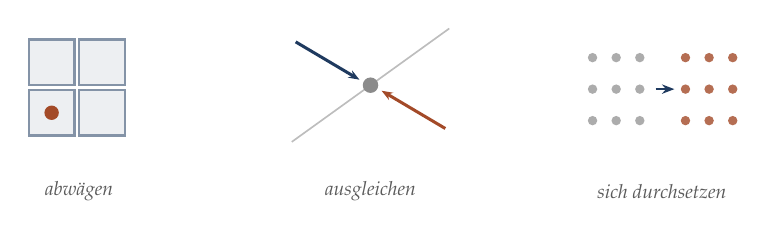
\begin{tikzpicture}[scale=1.0]
\begin{scope}[xshift=-3.7cm]
\foreach \x in {0,1} \foreach \y in {0,1}
  \draw[tief!55, line width=0.8pt, fill=tief!8] (\x*0.64-0.64,\y*0.64-0.64) rectangle ++(0.58,0.58);
\fill[akzent] (-0.35,-0.35) circle (2.6pt);
\node[font=\scriptsize\itshape, color=grau] at (0,-1.35) {abwägen};
\end{scope}
\begin{scope}
\draw[grau!40, line width=0.6pt] (-1.0,-0.72) -- (1.0,0.72);
\draw[tief, line width=1.1pt, -{Stealth[length=4pt]}] (-0.95,0.55) -- (-0.14,0.07);
\draw[akzent, line width=1.1pt, -{Stealth[length=4pt]}] (0.95,-0.55) -- (0.14,-0.07);
\fill[grau!70] (0,0) circle (2.8pt);
\node[font=\scriptsize\itshape, color=grau] at (0,-1.35) {ausgleichen};
\end{scope}
\begin{scope}[xshift=3.7cm]
\foreach \x in {-0.88,-0.58,-0.28} \foreach \y in {-0.45,-0.05,0.35}
  \fill[grau!50] (\x,\y) circle (1.7pt);
\foreach \x in {0.3,0.6,0.9} \foreach \y in {-0.45,-0.05,0.35}
  \fill[akzent!80] (\x,\y) circle (1.7pt);
\draw[tief, line width=0.9pt, -{Stealth[length=4.5pt]}] (-0.08,-0.05) -- (0.16,-0.05);
\node[font=\scriptsize\itshape, color=grau] at (0,-1.35) {sich durchsetzen};
\end{scope}
\end{tikzpicture}

\vspace{1.4cm}
{\large\color{grau} Von der Auszahlungsmatrix bis zum evolutionären Gleichgewicht}\\[6pt]
{\color{grau} Jeder Schritt erklärt. Mit vollständig durchgerechneten Übungsaufgaben.}\\[1.9cm]
{\small\color{grau} Stand der Forschung: August 2026}
\end{titlepage}
\thispagestyle{empty}
\vspace*{\fill}
\begin{flushleft}
{\small\color{grau}
\textbf{\color{tief}Mathematik von Grund auf} --- Band 21\\[2pt]
\textit{Wenn andere mitrechnen} $\cdot$ Spieltheorie\\[14pt]

Herausgeber und Urheber: Jürgen Maier\\[2pt]
Entstanden 2026 in Zusammenarbeit mit Claude (Anthropic); Konzeption, Vorgaben, Prüfung und Herausgeberschaft: Jürgen Maier.\\[14pt]

\textbf{Lizenz}\\[2pt]
Dieses Werk ist lizenziert unter einer Creative-Commons-Lizenz \textbf{Namensnennung -- Weitergabe unter gleichen Bedingungen 4.0 International (CC BY-SA 4.0)}. Sie dürfen das Werk vervielfältigen, verbreiten, bearbeiten und auch kommerziell nutzen, sofern Sie den Urheber nennen und Bearbeitungen unter derselben Lizenz weitergeben.\\[2pt]
Lizenztext: \texttt{https://creativecommons.org/licenses/by-sa/4.0/legalcode.de}\\[14pt]

\textbf{Quellen und Fassungen}\\[2pt]
Quelltexte, Simulationen, Fehlermeldungen und aktuelle Fassungen aller Bände:\\
\texttt{https://github.com/juergenmaier2026/mathematik-von-grund-auf}\\[2pt]
Dauerhaft archiviert bei Zenodo: \texttt{https://doi.org/10.5281/zenodo.23698547}\\[14pt]

\textbf{Zitiervorschlag}\\[2pt]
Maier, J. (2026). \textit{Mathematik von Grund auf, Band 21: Wenn andere mitrechnen}. Fassung 1.0.1. \texttt{https://doi.org/10.5281/zenodo.23698547}\\[14pt]

Satz: \LaTeX{} mit Palatino. Fassung 1.0.1, Oktober 2026. 236 Seiten.
}
\end{flushleft}
\vspace*{1.5cm}

\tableofcontents
\mainmatter

\chapter*{Vorwort}
\addcontentsline{toc}{chapter}{Vorwort}

\begin{merksatz}
\boxtitel{Wo die bisherigen Bände aufhören}
Band 19 fragte, wie man das Beste findet. Die Antwort setzte etwas voraus, das dort unausgesprochen blieb: dass die Welt nicht zurückrechnet.

\begin{center}
{\small
\renewcommand{\arraystretch}{1.5}
\begin{tabular}{@{}P{2.4cm}P{6.2cm}@{}}
\toprule
\textbf{Optimierung} & Man wählt unter Nebenbedingungen, die feststehen.\\
\textbf{Spieltheorie} & Die Nebenbedingungen sind Entscheidungen anderer --- die ihrerseits die eigenen voraussehen.\\
\bottomrule
\end{tabular}}
\end{center}

\begin{center}
\begin{minipage}{0.9\textwidth}
\textbf{Sobald jemand anderes mitrechnet, gibt es kein Optimum mehr, sondern nur noch ein Gleichgewicht.}
\end{minipage}
\end{center}

\begin{center}
\begin{minipage}{0.88\textwidth}
\kursiv{Das ist ein Begriffswechsel, kein Verfahrenswechsel --- und er verändert alles. Ein Optimum ist die beste Wahl. Ein Gleichgewicht ist eine Lage, aus der niemand allein ausbrechen will. \textbf{Die beiden fallen im Allgemeinen nicht zusammen}, und der berühmteste Fall dieses Bandes ist einer, in dem das Gleichgewicht für alle Beteiligten schlechter ist als eine andere erreichbare Lage.}
\end{minipage}
\end{center}
\end{merksatz}

\begin{merksatz}
\boxtitel{Drei Ergebnisse, die man nicht erwartet}
\begin{center}
{\small
\renewcommand{\arraystretch}{1.55}
\begin{tabular}{@{}P{1.0cm}P{7.4cm}@{}}
\toprule
$1$ & In jedem endlichen Zweipersonen-Nullsummenspiel gibt es einen Wert --- eine Zahl, die beide Seiten sich gegenseitig garantieren können. Vorher weiß niemand, wie der andere zieht; nachher bereut keiner. \kursiv{(Kapitel 2)}\\
$2$ & Jedes endliche Spiel hat ein Gleichgewicht --- beliebig viele Spieler, beliebige Auszahlungen. Der Beweis benutzt keine Rechnung, sondern einen Fixpunktsatz. \kursiv{(Kapitel 6)}\\
$3$ & Es gibt kein Abstimmungsverfahren für drei oder mehr Möglichkeiten, das drei naheliegende Forderungen erfüllt. Nicht \enquote{keines ist bekannt} --- es gibt keines. \kursiv{(Kapitel 12)}\\
\bottomrule
\end{tabular}}
\end{center}

\begin{center}
\begin{minipage}{0.88\textwidth}
\kursiv{Das erste Ergebnis ist der Ausgangspunkt des Fachs, das zweite seine Grundlage, das dritte seine schärfste Grenze. \textbf{Zwischen dem ersten und dem dritten liegen sechsundzwanzig Jahre} --- und der Weg von der Garantie zum Unmöglichkeitsbeweis ist die Erzählung dieses Bandes.}
\end{minipage}
\end{center}
\end{merksatz}

\begin{merksatz}
\boxtitel{Die sechs Teile}
\begin{center}
{\small
\renewcommand{\arraystretch}{1.5}
\begin{tabular}{@{}P{1.4cm}P{2.8cm}P{3.8cm}@{}}
\toprule
\textbf{Teil} & \textbf{Thema} & \textbf{Kapitel}\\
\midrule
I & Entgegengesetzte Interessen & $1$--$3$\\
II & Gleichgewichte & $4$--$6$\\
III & Über die Zeit & $7$--$8$\\
IV & Evolution & $9$--$10$\\
V & Regeln entwerfen & $11$--$14$\\
VI & Stand & $15$\\
\bottomrule
\end{tabular}}
\end{center}

\schritt{Der Leitfall}
Wie in den Bänden 18 bis 20 bleibt Neustadt der Schauplatz --- diesmal mit einem zweiten Haus.

\begin{center}
{\small
\renewcommand{\arraystretch}{1.5}
\begin{tabular}{@{}P{1.4cm}P{6.8cm}@{}}
\toprule
I & Klinikum und Marienhospital wählen Notarztstandorte.\\
II & Beide entscheiden über den Ausbau einer Spezialabteilung --- und über den Einsatz von Reserveantibiotika.\\
III & Verhandlungen mit den Kassen, Jahr für Jahr.\\
IV & Resistenzen: Bakterien spielen ebenfalls, ohne es zu wissen.\\
V & Dienstplan, Organverteilung, Ausschreibung.\\
\bottomrule
\end{tabular}}
\end{center}

\begin{center}
\begin{minipage}{0.88\textwidth}
\kursiv{Teil~IV setzt unmittelbar bei Band 18, Kapitel~14 an. Dort hieß es, das Wettrüsten zwischen Therapie und Resistenz sei im Kern ein Spiel --- und der Beweis blieb offen. \textbf{Er wird in Kapitel~10 nachgeholt}, mit derselben Gompertz-Kurve und denselben Mutationsraten.}
\end{minipage}
\end{center}
\end{merksatz}

\begin{warnung}
\boxtitelr{Drei Warnungen}
\begin{center}
{\small
\renewcommand{\arraystretch}{1.55}
\begin{tabular}{@{}P{2.2cm}P{6.4cm}@{}}
\toprule
\textbf{Erste} & Die Auszahlungen sind das Modell. Wer sie falsch ansetzt, bekommt eine tadellose Lösung für ein anderes Spiel. \kursiv{Das ist die häufigste Fehlanwendung des ganzen Fachs.}\\
\textbf{Zweite} & Die Theorie beschreibt, was rationale Spieler tun würden. Ob Menschen es tun, ist eine empirische Frage --- und die Antwort lautet oft nein. \kursiv{Kapitel 15 behandelt, was daraus folgt.}\\
\textbf{Dritte} & Ein Gleichgewicht ist keine Empfehlung. Es sagt, wo man landet, nicht wo man landen sollte.\\
\bottomrule
\end{tabular}}
\end{center}

\begin{center}
\begin{minipage}{0.88\textwidth}
\kursiv{Die dritte Warnung ist die wichtigste und wird am häufigsten überhört. Das Gefangenendilemma aus Kapitel~5 hat genau ein Gleichgewicht, und es ist für beide Spieler schlechter als die Zusammenarbeit. \textbf{Wer daraus schließt, man solle nicht zusammenarbeiten, hat den Satz gelesen und nicht verstanden.}}
\end{minipage}
\end{center}
\end{warnung}

\begin{merksatz}
\boxtitel{Was dieser Band voraussetzt}
\begin{center}
{\small
\renewcommand{\arraystretch}{1.48}
\begin{tabular}{@{}P{3.2cm}P{1.6cm}P{2.8cm}@{}}
\toprule
\textbf{Werkzeug} & \textbf{Band} & \textbf{gebraucht in}\\
\midrule
Wahrschein\-lichkeit & $12$ & Kapitel 3, 9\\
Lineare Optimierung & $19$ & Kapitel 3\\
Konvexität, Dualität & $19$ & Kapitel 3, 6\\
Differential\-gleichungen & $18$ & Kapitel 10\\
Fixpunktsätze & \textcolor{akzent}{---} & Kapitel 6\\
\bottomrule
\end{tabular}}
\end{center}

\begin{center}
\begin{minipage}{0.88\textwidth}
\kursiv{Die letzte Zeile ist die einzige echte Neuerung: Der Satz von Brouwer wird in Kapitel~6 eingeführt, nicht bewiesen --- und das ist die erste von neun Auslassungen, die der Anhang tabelliert. \textbf{Alles andere wird entweder hier entwickelt oder in einem früheren Band nachgeschlagen}, und wo etwas vorausgesetzt wird, steht die Fundstelle daneben.}
\end{minipage}
\end{center}
\end{merksatz}

\part{Entgegengesetzte Interessen}

\chapter{Was ein Spiel ist}

\section{Der Leitfall}

\begin{merksatz}
\boxtitel{Zwei Notarztstandorte}
Neustadt hat zwei Häuser: das Klinikum und das Marienhospital. Beide betreiben einen Notarztwagen und wählen dessen Standort --- Nord, Mitte oder Süd.

\begin{center}
\begin{minipage}{0.9\textwidth}
\textbf{Wer näher am Einsatzort steht, wird gerufen.} Der Anteil, den das eine Haus gewinnt, verliert das andere.
\end{minipage}
\end{center}

\schritt{Die Zahlen}
Anteil der Einsätze, die das Klinikum erreicht, in Prozent:

\begin{center}
{\small
\renewcommand{\arraystretch}{1.55}
\begin{tabular}{@{}P{2.2cm}P{1.6cm}P{1.6cm}P{1.6cm}@{}}
\toprule
\textbf{Klinikum} & \textbf{M.: N} & \textbf{M.: M} & \textbf{M.: S}\\
\midrule
Nord & $55$ & $40$ & $45$\\
Mitte & $60$ & $\mathbf{50}$ & $52$\\
Süd & $48$ & $38$ & $42$\\
\bottomrule
\end{tabular}}
\end{center}

\begin{center}
\begin{minipage}{0.88\textwidth}
\kursiv{Nur \kursiv{eine} Zahl je Feld genügt, weil das Marienhospital genau den Rest erhält. Bei $50$ für das Klinikum bleiben dem Marienhospital $50$. \textbf{Solche Spiele heißen Nullsummenspiele} --- nach einer Verschiebung der Skala summieren sich die Auszahlungen zu null.}
\end{minipage}
\end{center}
\end{merksatz}

\section{Die Bestandteile}

\begin{definition}
\boxtitelm{Definition 1.1 --- Spiel in Normalform}
Ein \Begriff{Spiel in Normalform} besteht aus
\begin{center}
{\small
\renewcommand{\arraystretch}{1.5}
\begin{tabular}{@{}P{2.4cm}P{6.2cm}@{}}
\toprule
\textbf{Spielern} & einer endlichen Menge $\{1,\ldots,n\}$\\
\textbf{Strategien} & für jeden Spieler $i$ einer Menge $\Str_i$\\
\textbf{Auszahlungen} & für jeden Spieler einer Funktion $\Aus_i: \Str_1\times\cdots\times\Str_n \to \R$\\
\bottomrule
\end{tabular}}
\end{center}
\end{definition}

\begin{merksatz}
\boxtitel{Was in dieser Definition steckt --- und was nicht}
\begin{center}
{\small
\renewcommand{\arraystretch}{1.52}
\begin{tabular}{@{}P{2.4cm}P{6.2cm}@{}}
\toprule
\textbf{Gleichzeitig} & Alle wählen, ohne die Wahl der anderen zu kennen. Kapitel~7 lockert das.\\
\textbf{Vollständig bekannt} & Jeder kennt alle Strategiemengen und alle Auszahlungen --- auch die der anderen.\\
\textbf{Eine Zahl je Ausgang} & Alles, was einem Spieler wichtig ist, steckt in einer einzigen Zahl.\\
\bottomrule
\end{tabular}}
\end{center}

\begin{center}
\begin{minipage}{0.9\textwidth}
\textbf{Die zweite Zeile ist eine starke Annahme.} Sie besagt nicht nur, dass jeder die Auszahlungen kennt, sondern auch, dass jeder weiß, dass jeder sie kennt --- und so fort.
\end{minipage}
\end{center}

\begin{center}
\begin{minipage}{0.88\textwidth}
\kursiv{Man nennt das \Begriff{allgemeines Wissen}. Ohne diese unendliche Kette bricht ein Teil der Schlüsse zusammen, die in Abschnitt 1.4 gezogen werden --- denn dort schließt Spieler A daraus, was B aus dem schließt, was A tut. \textbf{Die Annahme ist selten erfüllt und fast nie überprüft.}}
\end{minipage}
\end{center}

\schritt{Zur dritten Zeile}
Die Auszahlung ist kein Geldbetrag, sondern ein \Begriff{Nutzen}: eine Zahl, die die Vorlieben des Spielers vollständig ordnet.

\begin{center}
\begin{minipage}{0.88\textwidth}
\kursiv{Für das Klinikum steckt darin der Erlös, aber auch der Ruf, die Auslastung, die Zufriedenheit der Mitarbeiter --- alles in einer Zahl verrechnet. \textbf{Dass sich das überhaupt tun lässt, ist ein eigener Satz}, den von Neumann und Morgenstern 1944 bewiesen und den Kapitel~4 behandelt. Er verlangt Annahmen, die man sich ansehen sollte, bevor man ihm folgt.}
\end{minipage}
\end{center}
\end{merksatz}

\begin{definition}
\boxtitelm{Definition 1.2 --- Nullsummenspiel}
Ein Zweipersonenspiel heißt \Begriff{Nullsummenspiel}, wenn
\[ \Aus_1(s_1,s_2) + \Aus_2(s_1,s_2) = 0 \qquad\text{für alle } (s_1,s_2) . \]
\end{definition}

\begin{merksatz}
\boxtitel{Warum eine Matrix genügt}
Ist $\Aus_2 = -\Aus_1$, so ist das Spiel durch die Matrix von $\Aus_1$ vollständig beschrieben.

\begin{center}
\begin{minipage}{0.9\textwidth}
\textbf{Der Zeilenspieler will den Eintrag groß machen, der Spaltenspieler klein.}
\end{minipage}
\end{center}

\begin{center}
\begin{minipage}{0.88\textwidth}
\kursiv{Im Leitfall summieren sich die Anteile zu $100$, nicht zu null --- aber eine Verschiebung um $50$ macht daraus ein Nullsummenspiel, ohne irgendeine Entscheidung zu ändern. \textbf{Was zählt, ist die Gegenläufigkeit, nicht die Zahl null.} Man spricht deshalb oft allgemeiner von \Begriff{strikt kompetitiven} Spielen.}
\end{minipage}
\end{center}
\end{merksatz}

\section{Sich absichern}

\begin{merksatz}
\boxtitel{Die vorsichtige Rechnung}
Das Klinikum fragt sich: Was ist mir garantiert, wenn ich Zeile $r$ wähle und das Marienhospital anschließend das Schlimmste tut?

\begin{center}
{\small
\renewcommand{\arraystretch}{1.55}
\begin{tabular}{@{}P{2.0cm}P{1.4cm}P{1.4cm}P{1.4cm}P{2.0cm}@{}}
\toprule
& \textbf{N} & \textbf{M} & \textbf{S} & \textbf{Garantie}\\
\midrule
Nord & $55$ & $40$ & $45$ & $40$\\
Mitte & $60$ & $50$ & $52$ & $\mathbf{50}$\\
Süd & $48$ & $38$ & $42$ & $38$\\
\bottomrule
\end{tabular}}
\end{center}

\[ \text{Maximin} = \max_r \min_c a_{rc} = 50 \]

\schritt{Die andere Seite}
Das Marienhospital fragt: Was riskiere ich höchstens, wenn ich Spalte $c$ wähle?

\begin{center}
{\small
\renewcommand{\arraystretch}{1.55}
\begin{tabular}{@{}P{2.8cm}P{1.3cm}P{1.3cm}P{1.3cm}@{}}
\toprule
& \textbf{N} & \textbf{M} & \textbf{S}\\
\midrule
Spaltenmaximum & $60$ & $\mathbf{50}$ & $52$\\
\bottomrule
\end{tabular}}
\end{center}

\[ \text{Minimax} = \min_c \max_r a_{rc} = 50 \]
\end{merksatz}

\begin{merksatz}
\boxtitel{Satz 1.3 --- Maximin liegt nie über Minimax}
Für jede Matrix gilt
\[ \max_r \min_c a_{rc} \ \le\ \min_c \max_r a_{rc} . \]

\schritt{Beweis}
Seien $r^{*}$ und $c^{*}$ beliebig. Dann gilt
\[ \min_c a_{r^{*}c} \ \le\ a_{r^{*}c^{*}} \ \le\ \max_r a_{rc^{*}} . \]

\kursiv{Erste Ungleichung:} Das Minimum über alle $c$ ist höchstens der Wert bei $c^{*}$.\\
\kursiv{Zweite:} Der Wert bei $r^{*}$ ist höchstens das Maximum über alle $r$.

Die linke Seite hängt nicht von $c^{*}$ ab, die rechte nicht von $r^{*}$. Also gilt die Ungleichung auch für das Maximum links und das Minimum rechts. $\blacksquare$

\begin{center}
\begin{minipage}{0.88\textwidth}
\kursiv{Der Beweis ist drei Zeilen lang und benutzt nichts als die Definition von Maximum und Minimum. \textbf{Er gilt für jede Matrix, ohne jede Voraussetzung} --- und er sagt, dass die vorsichtige Garantie des einen nie besser ist als das schlimmste Zugeständnis des anderen.}
\end{minipage}
\end{center}
\end{merksatz}

\begin{definition}
\boxtitelm{Definition 1.4 --- Sattelpunkt}
Ein Feld $(r^{*},c^{*})$ heißt \Begriff{Sattelpunkt}, wenn es zugleich das Minimum seiner Zeile und das Maximum seiner Spalte ist.
\end{definition}

\begin{merksatz}
\boxtitel{Satz 1.5 --- Sattelpunkt heißt Gleichheit}
Ein Sattelpunkt existiert genau dann, wenn Maximin und Minimax übereinstimmen. Sein Wert ist dann dieser gemeinsame Wert.

\schritt{Beweis, Richtung eins}
Sei $(r^{*},c^{*})$ ein Sattelpunkt mit Wert $v = a_{r^{*}c^{*}}$.
\begin{align*}
\text{Maximin} &\ \ge\ \min_c a_{r^{*}c} = v && \text{($v$ ist Zeilenminimum)}\\
\text{Minimax} &\ \le\ \max_r a_{rc^{*}} = v && \text{($v$ ist Spaltenmaximum)}
\end{align*}
Zusammen mit Satz 1.3:
\[ v \le \text{Maximin} \le \text{Minimax} \le v \]
Also sind alle drei gleich. \checkmark

\schritt{Richtung zwei}
Gilt Maximin $=$ Minimax $= v$, so gibt es ein $r^{*}$ mit $\min_c a_{r^{*}c} = v$ und ein $c^{*}$ mit $\max_r a_{rc^{*}} = v$.

Dann ist
\[ v = \min_c a_{r^{*}c} \ \le\ a_{r^{*}c^{*}} \ \le\ \max_r a_{rc^{*}} = v , \]
also $a_{r^{*}c^{*}} = v$ --- und das Feld ist Zeilenminimum und Spaltenmaximum zugleich. $\blacksquare$
\end{merksatz}

\begin{merksatz}
\boxtitel{Der Leitfall hat einen}
\[ \text{Maximin} = \text{Minimax} = 50 \]

\begin{center}
{\small
\renewcommand{\arraystretch}{1.55}
\begin{tabular}{@{}P{2.2cm}P{1.2cm}P{1.2cm}P{1.2cm}P{1.9cm}@{}}
\toprule
& \textbf{N} & \textbf{M} & \textbf{S} & \textbf{Zeilenmin}\\
\midrule
Nord & $55$ & $40$ & $45$ & $40$\\
Mitte & $60$ & \cellcolor{akzent!18}$\mathbf{50}$ & $52$ & $\mathbf{50}$\\
Süd & $48$ & $38$ & $42$ & $38$\\
\midrule
\textbf{Spaltenmax} & $60$ & $\mathbf{50}$ & $52$ & \\
\bottomrule
\end{tabular}}
\end{center}

\begin{center}
\begin{minipage}{0.9\textwidth}
\textbf{Beide Häuser wählen Mitte, das Klinikum erreicht $50$ Prozent, und keines hat einen Grund, davon abzuweichen.}
\end{minipage}
\end{center}

\schritt{Was das bedeutet}
\begin{center}
{\small
\renewcommand{\arraystretch}{1.5}
\begin{tabular}{@{}P{2.6cm}P{6.0cm}@{}}
\toprule
\textbf{Kein Geheimnis nötig} & Das Klinikum könnte seine Wahl vorher bekanntgeben --- am Ergebnis änderte sich nichts.\\
\textbf{Kein Bedauern} & Nachdem beide gewählt haben, bereut keiner.\\
\textbf{Ein Wert} & Die Zahl $50$ beschreibt das Spiel vollständig.\\
\bottomrule
\end{tabular}}
\end{center}

\begin{center}
\begin{minipage}{0.88\textwidth}
\kursiv{Die erste Zeile ist das eigentliche Kennzeichen. In einem Spiel mit Sattelpunkt ist Verschwiegenheit wertlos --- und in einem ohne, wie wir in Kapitel~2 sehen werden, ist sie alles. \textbf{Der Sattelpunkt ist genau die Lage, in der Voraussagbarkeit nicht schadet.}}
\end{minipage}
\end{center}
\end{merksatz}

\section{Dominanz}

\begin{definition}
\boxtitelm{Definition 1.6}
Eine Strategie $s$ \Begriff{dominiert} eine Strategie $s'$ \Begriff{strikt}, wenn sie gegen \kursiv{jede} Wahl der Gegenseite echt besser abschneidet.
\end{definition}

\begin{merksatz}
\boxtitel{Der Leitfall löst sich auch so}
\schritt{Schritt 1 --- Für das Klinikum}
Zeile \enquote{Mitte} gegen Zeile \enquote{Nord}:
\[ 60 > 55, \qquad 50 > 40, \qquad 52 > 45 \]
\textbf{Mitte dominiert Nord strikt.} Ebenso Süd:
\[ 60 > 48, \qquad 50 > 38, \qquad 52 > 42 \]

\schritt{Schritt 2 --- Für das Marienhospital}
Es will kleine Werte. Spalte \enquote{M} gegen die anderen:
\[ 40 < 55, \quad 50 < 60, \quad 38 < 48 \qquad\text{(gegen N)} \]
\[ 40 < 45, \quad 50 < 52, \quad 38 < 42 \qquad\text{(gegen S)} \]
\textbf{Mitte dominiert auch hier strikt.}

\schritt{Schritt 3 --- Das Ergebnis}
\begin{center}
\begin{minipage}{0.9\textwidth}
\textbf{Beide Seiten haben eine Strategie, die immer besser ist.} Man braucht den Sattelpunkt gar nicht zu suchen.
\end{minipage}
\end{center}

\begin{center}
\begin{minipage}{0.88\textwidth}
\kursiv{Das ist hier ein glücklicher Sonderfall. \textbf{Dominanz ist die stärkste Art von Argument in diesem Band}, weil sie ohne jede Annahme über das Verhalten des Gegenübers auskommt: Man muss nicht unterstellen, dass er vernünftig handelt, sondern nur, dass man selbst es tut.}
\end{minipage}
\end{center}
\end{merksatz}

\begin{merksatz}
\boxtitel{Schrittweise streichen}
Meist dominiert nicht eine Strategie alle anderen, sondern nur einzelne. Dann streicht man und schaut erneut.

\schritt{Ein Beispiel}
\begin{center}
{\small
\renewcommand{\arraystretch}{1.5}
\begin{tabular}{@{}P{1.6cm}P{1.4cm}P{1.4cm}P{1.4cm}@{}}
\toprule
& \textbf{L} & \textbf{M} & \textbf{R}\\
\midrule
\textbf{O} & $4$ & $3$ & $7$\\
\textbf{U} & $2$ & $6$ & $5$\\
\bottomrule
\end{tabular}}
\end{center}

\kursiv{Für den Spaltenspieler:} L $(4;2)$ gegen R $(7;5)$ --- L ist in beiden Zeilen kleiner. \textbf{L dominiert R.} Streichen:

\begin{center}
{\small
\renewcommand{\arraystretch}{1.5}
\begin{tabular}{@{}P{1.6cm}P{1.4cm}P{1.4cm}@{}}
\toprule
& \textbf{L} & \textbf{M}\\
\midrule
\textbf{O} & $4$ & $3$\\
\textbf{U} & $2$ & $6$\\
\bottomrule
\end{tabular}}
\end{center}

\kursiv{Jetzt:} Keine weitere Dominanz. Zeilenminima $3$ und $2$, Spaltenmaxima $4$ und $6$.
\[ \text{Maximin} = 3 \ <\ 4 = \text{Minimax} \]

\begin{center}
\begin{minipage}{0.9\textwidth}
\textbf{Kein Sattelpunkt.} Die Dominanz half, reichte aber nicht.
\end{minipage}
\end{center}

\begin{center}
\begin{minipage}{0.88\textwidth}
\kursiv{Das ist der Normalfall, und er ist der Grund für Kapitel~2 und 3. Die Lücke zwischen $3$ und $4$ ist nicht zu schließen, solange man sich auf feste Wahlen beschränkt. \textbf{Man muss würfeln} --- und der Satz, der das rechtfertigt, ist der wichtigste dieses Teils.}
\end{minipage}
\end{center}
\end{merksatz}

\begin{warnung}
\boxtitelr{Strikt oder schwach --- ein Unterschied mit Folgen}
Dominiert $s$ die Strategie $s'$ nur \kursiv{schwach} --- also nirgends schlechter, irgendwo besser ---, so kann das Streichen Lösungen vernichten.

\begin{center}
{\small
\renewcommand{\arraystretch}{1.5}
\begin{tabular}{@{}P{1.6cm}P{1.4cm}P{1.4cm}@{}}
\toprule
& \textbf{L} & \textbf{R}\\
\midrule
\textbf{O} & $1$ & $1$\\
\textbf{U} & $0$ & $2$\\
\bottomrule
\end{tabular}}
\end{center}

\kursiv{Für den Spaltenspieler} dominiert L die Strategie R schwach: $1 \le 1$ und $0 < 2$.

\begin{center}
\begin{minipage}{0.9\textwidth}
\textbf{Streicht man R, so bleibt die Lösung $(\text{O},\text{L})$ mit Wert $1$.} Das Feld $(\text{O},\text{R})$ mit demselben Wert ist ebenfalls ein Sattelpunkt --- und wurde weggeworfen.
\end{minipage}
\end{center}

\begin{center}
\begin{minipage}{0.88\textwidth}
\kursiv{Beim Nullsummenspiel ist der Schaden gering, weil der Wert derselbe bleibt. \textbf{Bei den Spielen aus Teil~II ist er erheblich}: Dort kann schwache Dominanzelimination Gleichgewichte mit ganz verschiedenen Auszahlungen beseitigen, und sogar die \kursiv{Reihenfolge} des Streichens beeinflusst das Ergebnis. Strikte Dominanz hat diese Schwäche nicht.}
\end{minipage}
\end{center}
\end{warnung}

\section{Der Bruchfall}

\begin{warnung}
\boxtitelr{Was die Matrix verschweigt}
\begin{center}
{\small
\renewcommand{\arraystretch}{1.52}
\begin{tabular}{@{}P{2.4cm}P{6.2cm}@{}}
\toprule
\textbf{Woher die Zahlen} & Die Auszahlungen sind Schätzungen. Im Leitfall beruhen sie auf Fahrzeiten, Bevölkerungsdichte und Annahmen über die Disposition.\\
\textbf{Wer die Spieler sind} & Ein Haus ist kein Spieler --- Geschäftsführung, Chefärzte und Träger haben verschiedene Ziele.\\
\textbf{Was sonst geschieht} & Die Leitstelle disponiert nach eigenen Regeln. Sie ist ein dritter Beteiligter, der nicht in der Matrix steht.\\
\bottomrule
\end{tabular}}
\end{center}

\schritt{Zur zweiten Zeile}
\begin{center}
\begin{minipage}{0.88\textwidth}
\kursiv{Die Annahme, eine Organisation handle wie eine Person mit einer einzigen Zielfunktion, ist bequem und meist falsch. \textbf{Sie ist zugleich unvermeidlich}, wenn man überhaupt rechnen will --- und deshalb gehört zu jeder spieltheoretischen Analyse die Frage, wie empfindlich das Ergebnis auf diese Vereinfachung reagiert.}
\end{minipage}
\end{center}

\schritt{Und die Empfindlichkeit prüfen}
Im Leitfall liegt der Sattelpunkt bei $50$, die nächstbeste Zeile garantiert $40$.

\begin{center}
\begin{minipage}{0.9\textwidth}
\textbf{Der Abstand beträgt zehn Punkte.} Eine Schätzung, die um zwei oder drei danebenliegt, ändert nichts --- eine, die um zwölf danebenliegt, alles.
\end{minipage}
\end{center}

\begin{center}
\begin{minipage}{0.88\textwidth}
\kursiv{Diese Rechnung ist die Entsprechung der Schattenpreise und Gültigkeitsbereiche aus Band 19, Kapitel~5. \textbf{Sie sollte zu jeder Lösung dazugehören} und fehlt in den meisten Anwendungen --- was die erste Warnung des Vorworts erklärt.}
\end{minipage}
\end{center}
\end{warnung}

\section{Übungsaufgaben}

\begin{aufgabe}
\boxtitel{Aufgabe 1.1 --- Sattelpunkte finden}
Bestimmen Sie für jede Matrix Maximin, Minimax und gegebenenfalls den Sattelpunkt.
\begin{center}
{\small
\renewcommand{\arraystretch}{1.44}
\begin{tabular}{@{}P{1.0cm}P{2.6cm}P{1.0cm}P{2.6cm}@{}}
\toprule
(a) & $\begin{pmatrix}3&5\\2&4\end{pmatrix}$ & (b) & $\begin{pmatrix}1&4\\3&2\end{pmatrix}$\\[12pt]
(c) & $\begin{pmatrix}6&2&8\\4&5&7\\3&1&9\end{pmatrix}$ & (d) & $\begin{pmatrix}2&2\\2&2\end{pmatrix}$\\
\bottomrule
\end{tabular}}
\end{center}

\loesung
\schritt{(a)}
\begin{center}
\renewcommand{\arraystretch}{1.46}
\begin{tabular}{@{}P{2.2cm}P{1.1cm}P{1.1cm}P{1.9cm}@{}}
\toprule
& $c_1$ & $c_2$ & \textbf{Zeilenmin}\\
\midrule
$r_1$ & $3$ & $5$ & $\mathbf{3}$\\
$r_2$ & $2$ & $4$ & $2$\\
\midrule
\textbf{Spaltenmax} & $\mathbf{3}$ & $5$ & \\
\bottomrule
\end{tabular}
\end{center}

\[ \text{Maximin} = 3 = \text{Minimax} \quad\Longrightarrow\quad \text{Sattelpunkt bei } (r_1,c_1), \ v = 3 \]

\kursiv{Probe:} $3$ ist Minimum der Zeile $(3;5)$ \checkmark und Maximum der Spalte $(3;2)$ \checkmark

\schritt{(b)}
\begin{center}
\renewcommand{\arraystretch}{1.46}
\begin{tabular}{@{}P{2.2cm}P{1.1cm}P{1.1cm}P{1.9cm}@{}}
\toprule
& $c_1$ & $c_2$ & \textbf{Zeilenmin}\\
\midrule
$r_1$ & $1$ & $4$ & $1$\\
$r_2$ & $3$ & $2$ & $\mathbf{2}$\\
\midrule
\textbf{Spaltenmax} & $\mathbf{3}$ & $4$ & \\
\bottomrule
\end{tabular}
\end{center}

\[ \text{Maximin} = 2 \ <\ 3 = \text{Minimax} \]

\textcolor{akzent}{\textbf{Kein Sattelpunkt.}} Die Lücke beträgt $1$.

\schritt{(c)}
\begin{center}
\renewcommand{\arraystretch}{1.46}
\begin{tabular}{@{}P{2.2cm}P{1.0cm}P{1.0cm}P{1.0cm}P{1.9cm}@{}}
\toprule
& $c_1$ & $c_2$ & $c_3$ & \textbf{Zeilenmin}\\
\midrule
$r_1$ & $6$ & $2$ & $8$ & $2$\\
$r_2$ & $4$ & $5$ & $7$ & $\mathbf{4}$\\
$r_3$ & $3$ & $1$ & $9$ & $1$\\
\midrule
\textbf{Spaltenmax} & $6$ & $\mathbf{5}$ & $9$ & \\
\bottomrule
\end{tabular}
\end{center}

\[ \text{Maximin} = 4 \ <\ 5 = \text{Minimax} \]

\textcolor{akzent}{\textbf{Kein Sattelpunkt.}}

\schritt{(d)}
Alle Einträge gleich: Maximin $=$ Minimax $= 2$.

\begin{center}
\begin{minipage}{0.9\textwidth}
\textbf{Alle vier Felder sind Sattelpunkte.} Sattelpunkte sind nicht eindeutig.
\end{minipage}
\end{center}

\schritt{Die Übersicht}
\begin{center}
{\small
\renewcommand{\arraystretch}{1.48}
\begin{tabular}{@{}P{1.0cm}P{1.8cm}P{1.8cm}P{2.2cm}@{}}
\toprule
& \textbf{Maximin} & \textbf{Minimax} & \textbf{Sattelpunkt}\\
\midrule
(a) & $3$ & $3$ & \textcolor{gruen}{ja, eindeutig}\\
(b) & $2$ & $3$ & \textcolor{akzent}{nein}\\
(c) & $4$ & $5$ & \textcolor{akzent}{nein}\\
(d) & $2$ & $2$ & \textcolor{gruen}{ja, vier}\\
\bottomrule
\end{tabular}}
\end{center}

\begin{center}
\begin{minipage}{0.88\textwidth}
\kursiv{Zwei von vier Matrizen haben keinen Sattelpunkt --- und das ist typisch. \textbf{Bei zufällig gewählten $2\times2$-Matrizen liegt der Anteil bei zwei Dritteln}, bei größeren Matrizen sinkt er rasch. Kapitel~2 zeigt, dass sich die Lücke stets schließen lässt, wenn man Zufall zulässt.}
\end{minipage}
\end{center}
\end{aufgabe}

\begin{aufgabe}
\boxtitel{Aufgabe 1.2 --- Dominanz anwenden}
Vereinfachen Sie durch schrittweises Streichen strikt dominierter Strategien:
\[ \begin{pmatrix} 5 & 3 & 6 & 4\\ 7 & 4 & 8 & 5\\ 2 & 1 & 3 & 2 \end{pmatrix} \]

\loesung
\schritt{Schritt 1 --- Zeilen prüfen (Zeilenspieler maximiert)}
\kursiv{Zeile 2 gegen Zeile 1:} $7>5$, $4>3$, $8>6$, $5>4$ --- \textbf{Zeile 2 dominiert Zeile 1 strikt.}

\kursiv{Zeile 2 gegen Zeile 3:} $7>2$, $4>1$, $8>3$, $5>2$ --- \textbf{ebenfalls.}

Es bleibt nur Zeile 2:
\[ \begin{pmatrix} 7 & 4 & 8 & 5 \end{pmatrix} \]

\schritt{Schritt 2 --- Spalten prüfen (Spaltenspieler minimiert)}
\kursiv{Spalte 2} hat den kleinsten Wert $4$; sie dominiert alle anderen strikt:
\[ 4 < 7, \qquad 4 < 8, \qquad 4 < 5 \]

\schritt{Schritt 3 --- Das Ergebnis}
\[ \text{Lösung: } (r_2,c_2), \qquad v = 4 \]

\schritt{Schritt 4 --- Die Probe über Sattelpunkte}
\begin{center}
\renewcommand{\arraystretch}{1.46}
\begin{tabular}{@{}P{2.2cm}P{0.85cm}P{0.85cm}P{0.85cm}P{0.85cm}P{1.9cm}@{}}
\toprule
& $c_1$ & $c_2$ & $c_3$ & $c_4$ & \textbf{Zeilenmin}\\
\midrule
$r_1$ & $5$ & $3$ & $6$ & $4$ & $3$\\
$r_2$ & $7$ & $4$ & $8$ & $5$ & $\mathbf{4}$\\
$r_3$ & $2$ & $1$ & $3$ & $2$ & $1$\\
\midrule
\textbf{Spaltenmax} & $7$ & $\mathbf{4}$ & $8$ & $5$ & \\
\bottomrule
\end{tabular}
\end{center}

\[ \text{Maximin} = \text{Minimax} = 4 \quad \checkmark \]

\schritt{Schritt 5 --- Eine Beobachtung zur Reihenfolge}
Hätte man mit den Spalten begonnen, so wäre Spalte 2 ebenfalls sofort übrig geblieben --- und dann Zeile 2.

\begin{center}
\begin{minipage}{0.88\textwidth}
\kursiv{Das ist kein Zufall: \textbf{Bei strikter Dominanz ist das Ergebnis von der Reihenfolge unabhängig}, und die Menge der überlebenden Strategien ist eindeutig bestimmt. Bei schwacher Dominanz gilt das nicht, wie der Warnkasten in Abschnitt 1.4 zeigte. Der Beweis der Unabhängigkeit steht in Osborne und Rubinstein\zit{19}.}
\end{minipage}
\end{center}
\end{aufgabe}

\begin{aufgabe}
\boxtitel{Aufgabe 1.3 --- Die Empfindlichkeit prüfen}
Im Leitfall wurde der Wert $50$ für das Feld (Mitte, Mitte) geschätzt. Um wie viel darf die Schätzung danebenliegen, ohne dass sich die Lösung ändert?

\loesung
\schritt{Schritt 1 --- Was der Sattelpunkt verlangt}
Der Wert $a$ im Feld (Mitte, Mitte) muss
\begin{center}
{\small
\renewcommand{\arraystretch}{1.5}
\begin{tabular}{@{}P{3.4cm}P{5.0cm}@{}}
\toprule
Zeilenminimum sein & $a \le 60$ und $a \le 52$\\
Spalten\-maximum sein & $a \ge 40$ und $a \ge 38$\\
\bottomrule
\end{tabular}}
\end{center}

\schritt{Schritt 2 --- Der Bereich}
\[ 40 \ \le\ a \ \le\ 52 \]

\begin{center}
\begin{minipage}{0.9\textwidth}
\textbf{Die Schätzung darf um $10$ nach unten und um $2$ nach oben danebenliegen.}
\end{minipage}
\end{center}

\schritt{Schritt 3 --- Was außerhalb geschieht}
\kursiv{Bei $a = 55$:} Das Feld ist kein Zeilenminimum mehr ($55 > 52$).
\begin{center}
\renewcommand{\arraystretch}{1.46}
\begin{tabular}{@{}P{1.8cm}P{1.2cm}P{1.2cm}P{1.2cm}P{1.6cm}@{}}
\toprule
& N & M & S & \textbf{Min}\\
\midrule
Nord & $55$ & $40$ & $45$ & $40$\\
Mitte & $60$ & $55$ & $52$ & $\mathbf{52}$\\
Süd & $48$ & $38$ & $42$ & $38$\\
\midrule
\textbf{Max} & $60$ & $55$ & $\mathbf{52}$ & \\
\bottomrule
\end{tabular}
\end{center}

Maximin $=$ Minimax $= 52$ --- der Sattelpunkt wandert nach (Mitte, Süd).

\kursiv{Bei $a = 35$:} Das Feld ist kein Spaltenmaximum mehr ($35 < 40$).
\begin{center}
\renewcommand{\arraystretch}{1.46}
\begin{tabular}{@{}P{1.8cm}P{1.2cm}P{1.2cm}P{1.2cm}P{1.6cm}@{}}
\toprule
& N & M & S & \textbf{Min}\\
\midrule
Nord & $55$ & $40$ & $45$ & $40$\\
Mitte & $60$ & $35$ & $52$ & $35$\\
Süd & $48$ & $38$ & $42$ & $38$\\
\midrule
\textbf{Max} & $60$ & $40$ & $52$ & \\
\bottomrule
\end{tabular}
\end{center}

Maximin $= 40$, Minimax $= 40$ --- Sattelpunkt bei (Nord, Mitte).

\schritt{Schritt 4 --- Die Übersicht}
\begin{center}
{\small
\renewcommand{\arraystretch}{1.48}
\begin{tabular}{@{}P{2.0cm}P{2.6cm}P{2.4cm}@{}}
\toprule
$a$ & \textbf{Sattelpunkt} & \textbf{Wert}\\
\midrule
$<40$ & (Nord, Mitte) & $40$\\
$40\ldots52$ & (Mitte, Mitte) & $a$\\
$>52$ & (Mitte, Süd) & $52$\\
\bottomrule
\end{tabular}}
\end{center}

\begin{center}
\begin{minipage}{0.9\textwidth}
\textbf{Der Wert des Spiels ist eine stetige, stückweise lineare Funktion der geschätzten Größe --- und er bleibt beschränkt.}
\end{minipage}
\end{center}

\schritt{Schritt 5 --- Die Deutung}
\begin{center}
\begin{minipage}{0.88\textwidth}
\kursiv{Selbst eine grob falsche Schätzung verändert den Wert nur zwischen $40$ und $52$. \textbf{Die Entscheidung des Klinikums bleibt in allen drei Fällen dieselbe: Mitte oder Nord}, und beide liegen nahe beieinander. Das ist ein beruhigender Befund --- und keineswegs selbstverständlich, wie Kapitel~5 an Beispielen zeigen wird, in denen eine Änderung um eine Einheit die Lösung vollständig umwirft.}
\end{minipage}
\end{center}
\end{aufgabe}

\begin{geschichte}
\boxtitelg{Ein Schachsatz und ein Beweis für sich}
\Person{Ernst Zermelo} (1871--1953) hielt 1912 auf einem Mathematikerkongress einen Vortrag über das Schachspiel.

\begin{center}
\begin{minipage}{0.9\textwidth}
\kursiv{Sein Ergebnis: Im Schach gibt es eine bestimmte Lage --- entweder kann Weiß einen Sieg erzwingen, oder Schwarz, oder beide können ein Remis erzwingen. \textbf{Welche der drei zutrifft, ist bis heute unbekannt} und wird es vermutlich bleiben. Der Satz sagt, dass eine Antwort existiert, nicht welche.}
\end{minipage}
\end{center}

\schritt{Die Methode}
Zermelos Beweis arbeitet rückwärts vom Spielende --- das Verfahren, das Kapitel~7 als Rückwärtsinduktion behandelt.

\begin{center}
\begin{minipage}{0.9\textwidth}
\kursiv{Es ist bemerkenswert, dass die Spieltheorie mit einem Satz über ein Spiel mit vollständiger Information beginnt, das sich gerade \kursiv{nicht} mit Matrizen behandeln lässt. \textbf{Die Normalform kam später und von einer anderen Seite.}}
\end{minipage}
\end{center}

\schritt{Borel}
\Person{Émile Borel} (1871--1956) untersuchte ab 1921 Spiele mit gemischten Strategien und formulierte die Frage nach dem Minimax-Satz.

\begin{center}
\begin{minipage}{0.9\textwidth}
\kursiv{Er hielt die allgemeine Antwort für zweifelhaft und vermutete, dass es Spiele ohne Wert gibt. \textbf{Borel lag falsch}, wie von Neumann 1928 zeigte --- was Borel später ohne Umschweife einräumte. Seine Arbeiten enthalten aber die Begriffe, die dafür nötig waren.}
\end{minipage}
\end{center}

\schritt{Und die Vorgeschichte}
\Person{James Waldegrave} beschrieb 1713 in einem Brief die gemischte Gleichgewichtsstrategie für ein Kartenspiel namens \kursiv{Le Her}.

\begin{center}
\begin{minipage}{0.9\textwidth}
\kursiv{Es ist die erste bekannte Minimax-Lösung überhaupt --- zweihundert Jahre vor Borel, in einem Briefwechsel über ein Gesellschaftsspiel. Der Brief wurde erst 1968 als solcher erkannt. \textbf{Es ist wieder das Muster aus Band 20: Eine Entdeckung, die niemand veröffentlicht, wirkt nicht.}}
\end{minipage}
\end{center}
\end{geschichte}

\begin{forschung}
\boxtitelp{Wo die Normalform an Grenzen stößt}
\begin{center}
{\small
\renewcommand{\arraystretch}{1.45}
\begin{tabular}{@{}P{2.8cm}P{5.4cm}@{}}
\toprule
\textbf{Größe} & Schon Schach hat mehr Strategien, als das Weltall Atome hat. Die Normalform ist dort kein brauchbares Werkzeug.\\
\textbf{Knapper Verstand} & Spieler rechnen nicht beliebig tief. Modelle mit begrenzter Denktiefe sagen Verhalten besser vorher.\\
\textbf{Unvollständiges Wissen} & Wer die Auszahlungen des anderen nicht kennt, spielt ein anderes Spiel.\\
\bottomrule
\end{tabular}}
\end{center}

\schritt{Zur zweiten Zeile}
In Versuchen wählen Menschen selten das Gleichgewicht, sondern denken ein bis zwei Schritte weit.

\begin{center}
\begin{minipage}{0.88\textwidth}
\kursiv{Modelle mit Denktiefen von null bis drei sagen beobachtetes Verhalten deutlich besser vorher als die Gleichgewichtsanalyse. \textbf{Die Dominanzargumente aus Abschnitt 1.4 sind davon am wenigsten betroffen} --- eine strikt dominierte Strategie wird auch von wenig rechnenden Menschen gemieden. Je mehr Schritte ein Argument braucht, desto schlechter beschreibt es die Wirklichkeit.}
\end{minipage}
\end{center}

\schritt{Zur dritten Zeile}
\Person{John Harsanyi} zeigte 1967, wie sich Spiele mit unvollständigem Wissen in Spiele mit vollständigem, aber unvollkommenem Wissen umformen lassen.

\begin{center}
\begin{minipage}{0.88\textwidth}
\kursiv{Der Kunstgriff: Man führt einen Zufallszug der Natur ein, der die Eigenschaften der Spieler bestimmt. Damit wird das Problem behandelbar --- um den Preis einer Annahme über die Wahrscheinlichkeiten, die niemand beobachtet. \textbf{Harsanyi erhielt dafür 1994 den Nobelpreis}, gemeinsam mit Nash und Selten.}
\end{minipage}
\end{center}
\end{forschung}

\begin{merksatz}
\boxtitel{Was Sie jetzt können}
\begin{center}
\renewcommand{\arraystretch}{1.5}
\begin{tabular}{@{}P{3.0cm}P{5.6cm}@{}}
\toprule
\textbf{Definition 1.1} & Spieler, Strategien, Auszahlungen\\
\textbf{Definition 1.2} & Nullsumme: eine Matrix genügt\\
\textbf{Satz 1.3} & Maximin $\le$ Minimax, immer\\
\textbf{Satz 1.5} & Sattelpunkt $\iff$ Gleichheit\\
\textbf{Dominanz} & strikt streichen ist unbedenklich\\
\bottomrule
\end{tabular}
\end{center}

\begin{center}
\begin{minipage}{0.88\textwidth}
\kursiv{Zwei der vier Matrizen aus Aufgabe 1.1 hatten keinen Sattelpunkt. Das nächste Kapitel zeigt, dass die Lücke stets verschwindet, sobald man eine einzige Zutat erlaubt: den Zufall.}
\end{minipage}
\end{center}
\end{merksatz}

\chapter{Der Minimax-Satz}

\section{Ein Spiel ohne Sattelpunkt}

\begin{merksatz}
\boxtitel{Der Leitfall, verschärft}
Die Leitstelle hat ihre Disposition geändert: Sie ruft nicht mehr das nächstgelegene Fahrzeug, sondern wechselt zwischen zwei Regeln. Die Anteile sehen nun so aus:

\begin{center}
{\small
\renewcommand{\arraystretch}{1.55}
\begin{tabular}{@{}P{2.2cm}P{1.6cm}P{1.6cm}P{1.8cm}@{}}
\toprule
\textbf{Klinikum} & \textbf{M.: N} & \textbf{M.: S} & \textbf{Garantie}\\
\midrule
Nord & $60$ & $40$ & $\mathbf{40}$\\
Süd & $30$ & $70$ & $30$\\
\midrule
\textbf{Risiko} & $\mathbf{60}$ & $70$ & \\
\bottomrule
\end{tabular}}
\end{center}

\[ \text{Maximin} = 40 \ <\ 60 = \text{Minimax} \]

\begin{center}
\begin{minipage}{0.9\textwidth}
\textbf{Kein Sattelpunkt.} Jedes Feld lädt eine der beiden Seiten zum Wechseln ein.
\end{minipage}
\end{center}

\schritt{Die Unruhe nachvollzogen}
\begin{center}
{\small
\renewcommand{\arraystretch}{1.5}
\begin{tabular}{@{}P{2.2cm}P{6.4cm}@{}}
\toprule
$(\text{N},\text{N})$ & $60$ --- das Marienhospital wechselt nach Süd.\\
$(\text{N},\text{S})$ & $40$ --- das Klinikum wechselt nach Süd.\\
$(\text{S},\text{S})$ & $70$ --- das Marienhospital wechselt nach Nord.\\
$(\text{S},\text{N})$ & $30$ --- das Klinikum wechselt nach Nord.\\
\bottomrule
\end{tabular}}
\end{center}

\begin{center}
\begin{minipage}{0.9\textwidth}
\textbf{Der Kreis schließt sich.} Es gibt keine feste Wahl, bei der beide bleiben würden.
\end{minipage}
\end{center}

\begin{center}
\begin{minipage}{0.88\textwidth}
\kursiv{Das ist die Lage, in der Verschwiegenheit alles wert ist. Wüsste das Marienhospital, wo der Notarztwagen des Klinikums steht, so brächte es das Klinikum auf $40$ oder $30$. \textbf{Die Lösung kann also nicht in einer festen Wahl bestehen} --- sie muss unvorhersehbar sein.}
\end{minipage}
\end{center}
\end{merksatz}

\section{Gemischte Strategien}

\begin{definition}
\boxtitelm{Definition 2.1}
Eine \Begriff{gemischte Strategie} des Zeilenspielers ist ein Wahrscheinlichkeitsvektor
\[ \vek{p} = (p_1,\ldots,p_m), \qquad p_i \ge 0, \qquad \sum_i p_i = 1 . \]
Die Strategien aus Kapitel~1 heißen zur Unterscheidung \Begriff{rein}.
\end{definition}

\begin{merksatz}
\boxtitel{Die erwartete Auszahlung}
Spielen beide Seiten gemischt, so ist die erwartete Auszahlung
\[ \Aus(\vek p,\vek q) = \sum_{i}\sum_{j} p_i\,a_{ij}\,q_j = \vek p^{\!\top} A\,\vek q . \]

\schritt{Warum das der richtige Ansatz ist}
\begin{center}
{\small
\renewcommand{\arraystretch}{1.5}
\begin{tabular}{@{}P{2.8cm}P{5.8cm}@{}}
\toprule
\textbf{Unabhängig} & Beide würfeln getrennt, also multiplizieren sich die Wahrscheinlichkeiten.\\
\textbf{Linear} & Der Ausdruck ist in $\vek p$ linear bei festem $\vek q$ und umgekehrt.\\
\textbf{Erwartungswert} & Die Auszahlung ist der Nutzen aus Kapitel~1 --- über ihn darf man mitteln.\\
\bottomrule
\end{tabular}}
\end{center}

\begin{center}
\begin{minipage}{0.88\textwidth}
\kursiv{Die dritte Zeile ist keine Nebensächlichkeit. \textbf{Man darf nur dann Erwartungswerte bilden, wenn die Auszahlungen ein Nutzen im Sinne von Neumanns und Morgensterns sind} --- bei Geldbeträgen ist das im Allgemeinen falsch, weil der Nutzen von Geld nicht linear ist. Kapitel~4 behandelt, was genau dafür vorausgesetzt werden muss.}
\end{minipage}
\end{center}

\schritt{Die Linearität hat eine Folge}
Gegen eine feste gemischte Strategie $\vek q$ ist die beste Antwort stets unter den \kursiv{reinen} Strategien zu finden.

\kursiv{Grund:} $\Aus(\vek p,\vek q)$ ist ein gewichteter Mittelwert der Werte $\Aus(i,\vek q)$. Ein Mittelwert ist nie größer als sein größter Summand.

\begin{center}
\begin{minipage}{0.9\textwidth}
\textbf{Man muss also nur endlich viele Antworten prüfen} --- das macht alle folgenden Rechnungen erst möglich.
\end{minipage}
\end{center}
\end{merksatz}

\section{Der Satz}

\begin{merksatz}
\boxtitel{Satz 2.2 --- von Neumann, 1928}
Für jede reelle Matrix $A$ gilt
\[ \max_{\vek p} \min_{\vek q} \vek p^{\!\top} A\,\vek q \ =\ \min_{\vek q} \max_{\vek p} \vek p^{\!\top} A\,\vek q . \]
Den gemeinsamen Wert nennt man den \Begriff{Wert des Spiels}.

\begin{center}
\begin{minipage}{0.9\textwidth}
\textbf{Die Lücke aus Satz 1.3 verschwindet, sobald man mischen darf --- bei jeder Matrix, ohne Ausnahme.}
\end{minipage}
\end{center}

\begin{center}
\begin{minipage}{0.88\textwidth}
\kursiv{Das ist der Satz, mit dem die Spieltheorie beginnt. Er behauptet, dass jedes endliche Zweipersonen-Nullsummenspiel eine Zahl hat --- einen Wert, den sich beide Seiten gegenseitig garantieren können. \textbf{Weder Borel noch die Zeitgenossen hielten das für ausgemacht}; Borel vermutete das Gegenteil.}
\end{minipage}
\end{center}

\schritt{Was der Satz nicht sagt}
\begin{center}
{\small
\renewcommand{\arraystretch}{1.5}
\begin{tabular}{@{}P{2.4cm}P{6.2cm}@{}}
\toprule
\textbf{Keine Eindeutigkeit} & Es kann mehrere optimale Mischungen geben.\\
\textbf{Kein Verfahren} & Der ursprüngliche Beweis sagt nicht, wie man $\vek p$ findet. Kapitel~3 liefert das nach.\\
\textbf{Keine Garantie je Spiel} & Garantiert ist der Erwartungswert. Im Einzelfall kann es schlechter ausgehen.\\
\bottomrule
\end{tabular}}
\end{center}

\begin{center}
\begin{minipage}{0.88\textwidth}
\kursiv{Die dritte Zeile ist der praktisch wichtigste Vorbehalt. Der Notarztwagen steht an genau einem Ort, und an einem bestimmten Tag kann das Ergebnis $30$ oder $70$ sein. \textbf{Der Wert $50$ zeigt sich erst über viele Wiederholungen} --- und ein Spiel, das nur einmal stattfindet, hat zwar einen Wert, aber niemand erlebt ihn.}
\end{minipage}
\end{center}
\end{merksatz}

\section{Der Beweis für zwei mal zwei}

\begin{merksatz}
\boxtitel{Satz 2.3 --- die Ausgleichslösung}
Sei
\[ A = \begin{pmatrix} a & b\\ c & d\end{pmatrix} \]
ohne Sattelpunkt. Dann ist $N := a+d-b-c \ne 0$, und mit
\[ p = \frac{d-c}{N}, \qquad q = \frac{d-b}{N}, \qquad v = \frac{ad-bc}{N} \]
gilt: $\vek p = (p,\,1-p)$ und $\vek q = (q,\,1-q)$ sind optimal, und $v$ ist der Wert.

\schritt{Schritt 1 --- Der Ansatz}
Der Zeilenspieler sucht ein $p$, bei dem die Gegenseite \kursiv{nichts gewinnt}, egal was sie tut:
\[ \underbrace{p\,a + (1-p)\,c}_{\text{gegen Spalte 1}} \ =\ \underbrace{p\,b + (1-p)\,d}_{\text{gegen Spalte 2}} \]

\schritt{Schritt 2 --- Auflösen}
\begin{align*}
p\,a + c - p\,c &= p\,b + d - p\,d\\
p\,(a-c) - p\,(b-d) &= d-c\\
p\,(a-c-b+d) &= d-c\\
p &= \frac{d-c}{a+d-b-c} = \frac{d-c}{N}
\end{align*}

\schritt{Schritt 3 --- Der Wert}
Einsetzen in die linke Seite:
\begin{align*}
v &= \frac{d-c}{N}\,a + \left(1-\frac{d-c}{N}\right)c\\
&= \frac{a(d-c) + c\,(N - d + c)}{N}\\
&= \frac{ad-ac + c\,(a+d-b-c-d+c)}{N}\\
&= \frac{ad-ac + c\,(a-b)}{N}\\
&= \frac{ad-ac+ac-bc}{N} = \frac{ad-bc}{N}
\end{align*}

\begin{center}
\begin{minipage}{0.9\textwidth}
\textbf{Der Zähler ist die Determinante der Matrix.}
\end{minipage}
\end{center}

\schritt{Schritt 4 --- Warum $N \ne 0$}
Wäre $N = 0$, so gälte $a-b = c-d$. Dann hätten beide Zeilen dasselbe Gefälle, und man prüft nach: In diesem Fall besitzt die Matrix einen Sattelpunkt --- entgegen der Voraussetzung.

\schritt{Schritt 5 --- Warum $0 \le p \le 1$}
Ohne Sattelpunkt liegt eines der beiden Muster vor:
\begin{center}
{\small
\renewcommand{\arraystretch}{1.5}
\begin{tabular}{@{}P{2.6cm}P{3.0cm}P{2.4cm}@{}}
\toprule
\textbf{Muster} & \textbf{Bedingung} & $N$\\
\midrule
$a$ und $d$ groß & $a>b$, $a>c$, $d>b$, $d>c$ & $>0$\\
$b$ und $c$ groß & $a<b$, $a<c$, $d<b$, $d<c$ & $<0$\\
\bottomrule
\end{tabular}}
\end{center}

Im ersten Fall sind $d-c$ und $N$ beide positiv, und $N - (d-c) = a-b > 0$, also $p < 1$. Der zweite Fall läuft ebenso. \checkmark

\schritt{Schritt 6 --- Die Optimalität}
Mit diesem $p$ erhält der Zeilenspieler gegen \kursiv{jede} Spaltenwahl genau $v$ --- also auch gegen jede Mischung, denn die ist ein Mittelwert.

\[ \min_{\vek q} \vek p^{\!\top} A \vek q = v \quad\Longrightarrow\quad \max_{\vek p}\min_{\vek q} \ \ge\ v \]

Dieselbe Rechnung für den Spaltenspieler liefert
\[ \min_{\vek q}\max_{\vek p} \ \le\ v . \]

Mit Satz 1.3 --- der für Mischungen genauso gilt --- folgt Gleichheit. $\blacksquare$

\begin{center}
\begin{minipage}{0.88\textwidth}
\kursiv{Damit ist Satz 2.2 für den Fall $2\times2$ vollständig bewiesen --- ohne jedes Hilfsmittel außer einer linearen Gleichung. \textbf{Der allgemeine Fall braucht mehr}, und Kapitel~3 zeigt, dass er genau der Dualitätssatz aus Band 19 ist.}
\end{minipage}
\end{center}
\end{merksatz}

\begin{merksatz}
\boxtitel{Der Leitfall gelöst}
\[ A = \begin{pmatrix} 60 & 40\\ 30 & 70\end{pmatrix} \]

\schritt{Der Nenner}
\[ N = 60+70-40-30 = 60 \]

\schritt{Die Mischungen}
\[ p = \frac{70-30}{60} = \frac{40}{60} = \frac23, \qquad q = \frac{70-40}{60} = \frac{30}{60} = \frac12 \]

\schritt{Der Wert}
\[ v = \frac{60\cdot70 - 40\cdot30}{60} = \frac{4200-1200}{60} = \frac{3000}{60} = 50 \]

\schritt{Die Proben}
\kursiv{Klinikum, gegen Nord:} $\tfrac23\cdot60 + \tfrac13\cdot30 = 40+10 = 50$ \checkmark\\
\kursiv{Klinikum, gegen Süd:} $\tfrac23\cdot40 + \tfrac13\cdot70 = \tfrac{80}{3}+\tfrac{70}{3} = 50$ \checkmark\\
\kursiv{Marienhospital, gegen Nord:} $\tfrac12\cdot60+\tfrac12\cdot40 = 50$ \checkmark\\
\kursiv{Marienhospital, gegen Süd:} $\tfrac12\cdot30+\tfrac12\cdot70 = 50$ \checkmark

\schritt{Die Einordnung}
\begin{center}
{\small
\renewcommand{\arraystretch}{1.5}
\begin{tabular}{@{}P{2.6cm}P{1.8cm}P{2.8cm}@{}}
\toprule
& \textbf{Wert} & \\
\midrule
Maximin (rein) & $40$ & Kapitel 1\\
\textbf{Wert (gemischt)} & $\mathbf{50}$ & dieses Kapitel\\
Minimax (rein) & $60$ & Kapitel 1\\
\bottomrule
\end{tabular}}
\end{center}

\begin{center}
\begin{minipage}{0.9\textwidth}
\textbf{Das Mischen bringt dem Klinikum zehn Punkte und kostet das Marienhospital ebenso viel.} Beide gewinnen dasselbe, was sie vorher an Vorsicht verloren.
\end{minipage}
\end{center}

\begin{center}
\begin{minipage}{0.88\textwidth}
\kursiv{Bemerkenswert an der Lösung ist die Ungleichheit der Mischungen: Das Klinikum steht in zwei von drei Fällen im Norden, das Marienhospital wechselt hälftig. \textbf{Die eigene optimale Mischung hängt nicht von den eigenen Auszahlungen ab, sondern von denen des Gegners} --- $p$ wird so gewählt, dass \kursiv{der andere} gleichgültig wird. Das ist eine der befremdlichsten Eigenschaften der Lösung, und Abschnitt 2.6 kommt darauf zurück.}
\end{minipage}
\end{center}
\end{merksatz}

\section{Der Preis der Offenheit}

\begin{merksatz}
\boxtitel{Drei Fälle}
\begin{center}
{\small
\renewcommand{\arraystretch}{1.52}
\begin{tabular}{@{}P{3.0cm}P{2.0cm}P{3.2cm}@{}}
\toprule
\textbf{Wer sich festlegt} & \textbf{Klinikum bekommt} & \\
\midrule
Klinikum nennt den Standort & $40$ & Maximin\\
\textbf{niemand} & $\mathbf{50}$ & Wert\\
Marienhospital nennt ihn & $60$ & Minimax\\
\bottomrule
\end{tabular}}
\end{center}

\begin{center}
\begin{minipage}{0.9\textwidth}
\textbf{Wer seinen gezogenen Standort preisgibt, zahlt zehn Punkte.}
\end{minipage}
\end{center}

\schritt{Und nun der überraschende Teil}
Was geschieht, wenn das Klinikum nicht den Standort, sondern \kursiv{die Mischung} bekanntgibt --- also offen sagt: \enquote{Wir stehen in zwei von drei Fällen im Norden, ausgewürfelt}?

\begin{center}
\renewcommand{\arraystretch}{1.5}
\begin{tabular}{@{}P{3.2cm}P{2.0cm}P{2.4cm}@{}}
\toprule
\textbf{Antwort} & \textbf{Ergebnis} & \\
\midrule
Marienhospital: Nord & $50$ & \\
Marienhospital: Süd & $50$ & \\
jede Mischung & $50$ & \\
\bottomrule
\end{tabular}
\end{center}

\begin{center}
\begin{minipage}{0.9\textwidth}
\textbf{Die Bekanntgabe der optimalen Mischung kostet nichts.} Das Marienhospital kann daraus keinen Vorteil ziehen.
\end{minipage}
\end{center}

\begin{center}
\begin{minipage}{0.88\textwidth}
\kursiv{Das ist der am häufigsten missverstandene Punkt des ganzen Kapitels. \textbf{Geheim bleiben muss der Ausgang des Würfels, nicht der Würfel.} Man darf seine Strategie veröffentlichen --- und genau das geschieht in der Praxis, etwa bei Zollkontrollen oder Stichprobenprüfungen, deren Quoten bekanntgegeben werden, ohne dass jemand weiß, wen es trifft.}
\end{minipage}
\end{center}

\schritt{Warum das so ist}
Die optimale Mischung macht die Gegenseite gleichgültig --- genau das war der Ansatz in Schritt 1 des Beweises.

\begin{center}
\begin{minipage}{0.88\textwidth}
\kursiv{Und daraus folgt zugleich die Umkehrung: \textbf{Jede \kursiv{nicht} optimale Mischung darf man nicht bekanntgeben}, denn dann hat die Gegenseite eine echt bessere Antwort. Die Bekanntgabe ist nur bei der Gleichgewichtsmischung folgenlos.}
\end{minipage}
\end{center}
\end{merksatz}

\section{Der Bruchfall}

\begin{warnung}
\boxtitelr{Vier Vorbehalte}
\begin{center}
{\small
\renewcommand{\arraystretch}{1.52}
\begin{tabular}{@{}P{2.4cm}P{6.2cm}@{}}
\toprule
\textbf{Echter Zufall nötig} & Ein vorhersehbarer Wechsel ist keine Mischung. Wer abwechselnd Nord und Süd fährt, ist nach zwei Tagen durchschaut.\\
\textbf{Nur der Erwartungswert} & Im Einzelfall kann es beliebig schlecht ausgehen.\\
\textbf{Nur Nullsummenspiele} & Satz 2.2 gilt für strikte Gegnerschaft. Bei gemeinsamen Interessen versagt er --- Teil~II.\\
\textbf{Endlich} & Bei unendlichen Strategiemengen kann der Wert fehlen.\\
\bottomrule
\end{tabular}}
\end{center}

\schritt{Zur ersten Zeile}
\begin{center}
\begin{minipage}{0.88\textwidth}
\kursiv{Menschen erzeugen keinen Zufall. In Versuchen wechseln sie zu häufig --- eine Folge von fünf gleichen Ergebnissen erscheint ihnen unzufällig, obwohl sie es nicht ist. \textbf{Ein Gegner, der dieses Muster kennt, schlägt jeden menschlichen \enquote{Zufall}}, und genau darauf beruhen Programme, die Schere-Stein-Papier gegen Menschen gewinnen. Wer mischen will, braucht ein Hilfsmittel.}
\end{minipage}
\end{center}

\schritt{Zur vierten Zeile}
Bei unendlich vielen Strategien kann es geschehen, dass Maximin und Minimax verschieden bleiben.

\begin{center}
\begin{minipage}{0.88\textwidth}
\kursiv{Ein bekanntes Beispiel: Beide nennen eine natürliche Zahl, wer die größere nennt, gewinnt. Es gibt keine optimale Strategie, weil es keine größte Zahl gibt. \textbf{Für stetige Spiele auf beschränkten Bereichen gilt der Satz weiterhin} --- unter Stetigkeitsannahmen, die Glicksberg 1952 bewies. Die Endlichkeit ist also nicht wesentlich, die Beschränktheit schon.}
\end{minipage}
\end{center}
\end{warnung}

\section{Übungsaufgaben}

\begin{aufgabe}
\boxtitel{Aufgabe 2.1 --- Die Lücke schließen}
Lösen Sie die Matrix aus Aufgabe 1.1(b), die keinen Sattelpunkt hatte:
\[ A = \begin{pmatrix} 1 & 4\\ 3 & 2\end{pmatrix} \]

\loesung
\schritt{Schritt 1 --- Prüfen, dass kein Sattelpunkt vorliegt}
Zeilenminima $1$ und $2$, Spaltenmaxima $3$ und $4$.
\[ \text{Maximin} = 2 \ <\ 3 = \text{Minimax} \quad \checkmark \]

\schritt{Schritt 2 --- Der Nenner}
\[ N = a+d-b-c = 1+2-4-3 = -4 \]

\begin{center}
\begin{minipage}{0.86\textwidth}
\kursiv{Hier liegt das zweite Muster aus Schritt 5 des Beweises vor: die Nebendiagonale ist groß. Der Nenner ist negativ, und die Formeln gelten unverändert.}
\end{minipage}
\end{center}

\schritt{Schritt 3 --- Die Mischungen}
\[ p = \frac{d-c}{N} = \frac{2-3}{-4} = \frac{-1}{-4} = \frac14 \]
\[ q = \frac{d-b}{N} = \frac{2-4}{-4} = \frac{-2}{-4} = \frac12 \]

\schritt{Schritt 4 --- Der Wert}
\[ v = \frac{ad-bc}{N} = \frac{1\cdot2 - 4\cdot3}{-4} = \frac{2-12}{-4} = \frac{-10}{-4} = \frac52 = 2{,}5 \]

\schritt{Schritt 5 --- Die Proben}
\kursiv{Zeilenspieler gegen Spalte 1:}
\[ \tfrac14\cdot1 + \tfrac34\cdot3 = \tfrac14 + \tfrac94 = \tfrac{10}{4} = 2{,}5 \quad \checkmark \]
\kursiv{gegen Spalte 2:}
\[ \tfrac14\cdot4 + \tfrac34\cdot2 = 1 + 1{,}5 = 2{,}5 \quad \checkmark \]
\kursiv{Spaltenspieler gegen Zeile 1:}
\[ \tfrac12\cdot1 + \tfrac12\cdot4 = 2{,}5 \quad \checkmark \]
\kursiv{gegen Zeile 2:}
\[ \tfrac12\cdot3 + \tfrac12\cdot2 = 2{,}5 \quad \checkmark \]

\schritt{Schritt 6 --- Die Einordnung}
\begin{center}
\renewcommand{\arraystretch}{1.48}
\begin{tabular}{@{}P{2.4cm}P{1.8cm}P{2.6cm}@{}}
\toprule
& \textbf{Wert} & \\
\midrule
Maximin & $2$ & \\
\textbf{Wert} & $\mathbf{2{,}5}$ & genau in der Mitte\\
Minimax & $3$ & \\
\bottomrule
\end{tabular}
\end{center}

\begin{center}
\begin{minipage}{0.88\textwidth}
\kursiv{Dass der Wert hier genau in der Mitte liegt, ist Zufall und nicht die Regel --- im Leitfall lag er bei $50$ zwischen $40$ und $60$, also ebenfalls mittig, aber das war eine Folge der symmetrischen Zahlen. \textbf{Allgemein liegt der Wert irgendwo im Intervall}, wie Aufgabe 2.2 zeigt.}
\end{minipage}
\end{center}
\end{aufgabe}

\begin{aufgabe}
\boxtitel{Aufgabe 2.2 --- Erst streichen, dann mischen}
Lösen Sie die Matrix aus Aufgabe 1.1(c):
\[ A = \begin{pmatrix} 6 & 2 & 8\\ 4 & 5 & 7\\ 3 & 1 & 9 \end{pmatrix} \]

\loesung
\schritt{Schritt 1 --- Dominanz bei den Spalten}
Der Spaltenspieler minimiert. Spalte 2 gegen Spalte 3:
\[ 2 < 8, \qquad 5 < 7, \qquad 1 < 9 \]
\textbf{Spalte 2 dominiert Spalte 3 strikt.} Streichen:
\[ \begin{pmatrix} 6 & 2\\ 4 & 5\\ 3 & 1 \end{pmatrix} \]

\schritt{Schritt 2 --- Dominanz bei den Zeilen}
Zeile 1 gegen Zeile 3:
\[ 6 > 3, \qquad 2 > 1 \]
\textbf{Zeile 1 dominiert Zeile 3 strikt.} Streichen:
\[ \begin{pmatrix} 6 & 2\\ 4 & 5 \end{pmatrix} \]

\begin{center}
\begin{minipage}{0.86\textwidth}
\kursiv{Man beachte die Reihenfolge: Zeile 3 war in der \kursiv{ursprünglichen} Matrix nicht dominiert, denn dort galt $8 < 9$. \textbf{Erst das Streichen der dritten Spalte machte die Dominanz sichtbar} --- und das ist der Grund, warum man abwechselnd vorgeht und nach jedem Streichen erneut prüft.}
\end{minipage}
\end{center}

\schritt{Schritt 3 --- Kein Sattelpunkt im Rest}
Zeilenminima $2$ und $4$, Spaltenmaxima $6$ und $5$.
\[ \text{Maximin} = 4 \ <\ 5 = \text{Minimax} \]

\schritt{Schritt 4 --- Die Lösung}
\[ N = 6+5-2-4 = 5 \]
\[ p = \frac{5-4}{5} = \frac15, \qquad q = \frac{5-2}{5} = \frac35 \]
\[ v = \frac{6\cdot5 - 2\cdot4}{5} = \frac{30-8}{5} = \frac{22}{5} = 4{,}4 \]

\schritt{Schritt 5 --- Die Proben}
\kursiv{Zeilenspieler:}
\[ \tfrac15\cdot6 + \tfrac45\cdot4 = \tfrac{6}{5}+\tfrac{16}{5} = \tfrac{22}{5} \quad \checkmark \]
\[ \tfrac15\cdot2 + \tfrac45\cdot5 = \tfrac{2}{5}+\tfrac{20}{5} = \tfrac{22}{5} \quad \checkmark \]
\kursiv{Spaltenspieler:}
\[ \tfrac35\cdot6 + \tfrac25\cdot2 = \tfrac{18}{5}+\tfrac{4}{5} = \tfrac{22}{5} \quad \checkmark \]
\[ \tfrac35\cdot4 + \tfrac25\cdot5 = \tfrac{12}{5}+\tfrac{10}{5} = \tfrac{22}{5} \quad \checkmark \]

\schritt{Schritt 6 --- Zurück zur vollen Matrix}
Die Lösung lautet für das ursprüngliche Spiel:
\begin{center}
{\small
\renewcommand{\arraystretch}{1.48}
\begin{tabular}{@{}P{2.4cm}P{3.0cm}P{2.6cm}@{}}
\toprule
\textbf{Spieler} & \textbf{Mischung} & \\
\midrule
Zeile & $(\tfrac15,\ \tfrac45,\ 0)$ & Zeile 3 ungenutzt\\
Spalte & $(\tfrac35,\ \tfrac25,\ 0)$ & Spalte 3 ungenutzt\\
\bottomrule
\end{tabular}}
\end{center}

\schritt{Schritt 7 --- Die abschließende Probe}
Man muss prüfen, dass die gestrichenen Strategien auch gegen die Lösung nichts taugen.

\kursiv{Zeile 3 gegen $\vek q = (\tfrac35,\tfrac25,0)$:}
\[ \tfrac35\cdot3 + \tfrac25\cdot1 = \tfrac{9}{5}+\tfrac{2}{5} = \tfrac{11}{5} = 2{,}2 \ <\ 4{,}4 \quad \checkmark \]

\kursiv{Spalte 3 gegen $\vek p = (\tfrac15,\tfrac45,0)$:}
\[ \tfrac15\cdot8 + \tfrac45\cdot7 = \tfrac{8}{5}+\tfrac{28}{5} = \tfrac{36}{5} = 7{,}2 \ >\ 4{,}4 \quad \checkmark \]

\begin{center}
\begin{minipage}{0.88\textwidth}
\kursiv{Die letzte Probe ist nicht überflüssig: Sie bestätigt, dass die Lösung des verkleinerten Spiels auch das volle Spiel löst. \textbf{Bei strikter Dominanz ist das stets der Fall}, und genau deshalb darf man streichen. Der Wert des vollen Spiels beträgt ebenfalls $4{,}4$ --- und er liegt \kursiv{nicht} in der Mitte zwischen $4$ und $5$.}
\end{minipage}
\end{center}
\end{aufgabe}

\begin{aufgabe}
\boxtitel{Aufgabe 2.3 --- Was Offenheit kostet}
Im Leitfall ($A = \begin{psmallmatrix}60&40\\30&70\end{psmallmatrix}$) wird das Klinikum gezwungen, seine Mischung $\vek p = (p,1-p)$ vorab bekanntzugeben. Welches $p$ wählt es, und was bekommt es?

\loesung
\schritt{Schritt 1 --- Die Antwort des Gegners}
Das Marienhospital kennt $p$ und wählt die für das Klinikum schlechtere Spalte:
\begin{center}
{\small
\renewcommand{\arraystretch}{1.5}
\begin{tabular}{@{}P{2.2cm}P{4.0cm}@{}}
\toprule
\textbf{Nord} & $f_N(p) = 60p + 30(1-p) = 30 + 30p$\\
\textbf{Süd} & $f_S(p) = 40p + 70(1-p) = 70 - 30p$\\
\bottomrule
\end{tabular}}
\end{center}

Das Klinikum erhält $\min\{f_N(p),\,f_S(p)\}$.

\schritt{Schritt 2 --- Die Funktion zeichnen}
\begin{center}
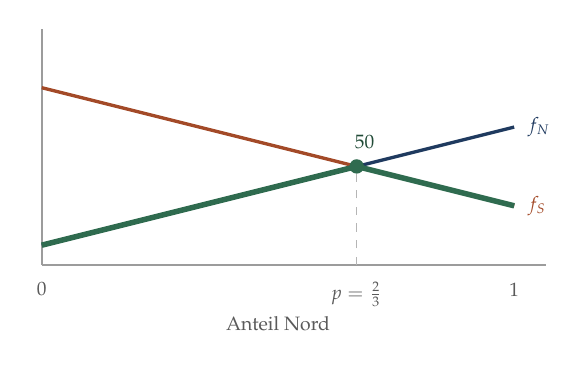
\begin{tikzpicture}[scale=1.0]
\draw[grau!60, line width=0.7pt] (0,0) -- (6.4,0);
\draw[grau!60, line width=0.7pt] (0,0) -- (0,3.0);
% f_N: 30+30p, skaliert: y = (wert-25)/20
\draw[tief, line width=1.2pt] (0,0.25) -- (6,1.75);
% f_S: 70-30p
\draw[akzent, line width=1.2pt] (0,2.25) -- (6,0.75);
% Minimum dick
\draw[gruen, line width=2.0pt] (0,0.25) -- (4,1.25);
\draw[gruen, line width=2.0pt] (4,1.25) -- (6,0.75);
\fill[gruen] (4,1.25) circle (2.6pt);
\draw[grau!45, line width=0.5pt, dashed] (4,0) -- (4,1.25);
\node[font=\scriptsize, color=tief, anchor=west] at (6.05,1.75) {$f_N$};
\node[font=\scriptsize, color=akzent, anchor=west] at (6.05,0.75) {$f_S$};
\node[font=\scriptsize, color=gruen!70!black, anchor=south] at (4.1,1.35) {$50$};
\node[font=\scriptsize, color=grau, anchor=north] at (4,-0.1) {$p=\frac23$};
\node[font=\scriptsize, color=grau, anchor=north] at (0,-0.1) {$0$};
\node[font=\scriptsize, color=grau, anchor=north] at (6,-0.1) {$1$};
\node[font=\scriptsize, color=grau] at (3.0,-0.75) {Anteil Nord};
\end{tikzpicture}
\end{center}

\schritt{Schritt 3 --- Das Maximum der unteren Hülle}
Die untere Hülle steigt, solange $f_N < f_S$, und fällt danach. Das Maximum liegt am Schnittpunkt:
\[ 30+30p = 70-30p \quad\Longrightarrow\quad 60p = 40 \quad\Longrightarrow\quad p = \tfrac23 \]
\[ v = 30 + 30\cdot\tfrac23 = 30+20 = 50 \]

\schritt{Schritt 4 --- Das Ergebnis}
\begin{center}
\begin{minipage}{0.9\textwidth}
\textbf{Das Klinikum wählt $p = \frac23$ und erhält $50$ --- genau so viel wie ohne Bekanntgabe.}
\end{minipage}
\end{center}

\schritt{Schritt 5 --- Der Vergleich der drei Lagen}
\begin{center}
{\small
\renewcommand{\arraystretch}{1.5}
\begin{tabular}{@{}P{3.4cm}P{2.0cm}P{2.4cm}@{}}
\toprule
\textbf{Das Klinikum gibt bekannt} & \textbf{bekommt} & \\
\midrule
nichts & $50$ & \\
die Mischung & $\mathbf{50}$ & \textcolor{gruen}{kostenlos}\\
den gezogenen Standort & $40$ & \textcolor{akzent}{$-10$}\\
\bottomrule
\end{tabular}}
\end{center}

\schritt{Schritt 6 --- Warum das so ist}
Die Kurve $\min\{f_N,f_S\}$ hat ihr Maximum genau dort, wo beide Geraden sich schneiden --- also dort, wo die Gegenseite gleichgültig ist.

\begin{center}
\begin{minipage}{0.88\textwidth}
\kursiv{\textbf{Das ist die zweite, anschauliche Herleitung von Satz 2.3}: Man zeichnet für jede gegnerische Antwort eine Gerade und sucht den höchsten Punkt der unteren Hülle. Diese Hülle ist stückweise linear und konkav --- die Konstruktion aus Band 19, Kapitel~7. \textbf{Damit ist der Minimax-Satz im Kern ein Konvexitätsargument}, und Kapitel~3 macht diesen Zusammenhang vollständig.}
\end{minipage}
\end{center}

\schritt{Schritt 7 --- Ein Gegenbeispiel zur Vorsicht}
Gäbe das Klinikum eine \kursiv{andere} Mischung bekannt, etwa $p = 0{,}9$:
\[ f_N(0{,}9) = 30+27 = 57, \qquad f_S(0{,}9) = 70-27 = 43 \]
Das Marienhospital wählt Süd, und das Klinikum erhält $43$.

\begin{center}
\begin{minipage}{0.86\textwidth}
\kursiv{\textbf{Die Bekanntgabe ist also nur bei der optimalen Mischung folgenlos.} Jede andere Mischung, offengelegt, kostet --- und zwar umso mehr, je weiter sie vom Schnittpunkt entfernt liegt.}
\end{minipage}
\end{center}
\end{aufgabe}

\begin{geschichte}
\boxtitelg{Ein Satz und ein langer Schatten}
\Person{John von Neumann} (1903--1957) bewies den Satz 1926 und veröffentlichte ihn 1928 in den \kursiv{Mathematischen Annalen} unter dem Titel \enquote{Zur Theorie der Gesellschaftsspiele}.

\begin{center}
\begin{minipage}{0.9\textwidth}
\kursiv{Er war dreiundzwanzig. Der Beweis benutzte den Brouwerschen Fixpunktsatz --- ein Werkzeug aus der Topologie, das mit Gesellschaftsspielen nichts zu tun hat. Von Neumann sagte später, ohne diesen Satz hätte es keine Spieltheorie gegeben, und es ist bemerkenswert, dass derselbe Satz 1950 auch Nashs Ergebnis tragen sollte.}
\end{minipage}
\end{center}

\schritt{Die Einschätzung des Verfassers}
Von Neumann hielt den Minimax-Satz für das Fundament und äußerte, ohne ihn gebe es \enquote{nichts zu beweisen}.

\begin{center}
\begin{minipage}{0.9\textwidth}
\kursiv{Das war zugleich eine Grenzziehung: Er hielt Nichtnullsummenspiele für begrifflich ungeklärt und stand Nashs späterem Ergebnis skeptisch gegenüber. \textbf{Der Mann, der das Fach begründete, hielt seine wichtigste Erweiterung für einen Nebenweg} --- Kapitel~4 erzählt, wie das Gespräch ausging.}
\end{minipage}
\end{center}

\schritt{Das Buch}
1944 erschien \kursiv{Theory of Games and Economic Behavior}, gemeinsam mit dem Ökonomen \Person{Oskar Morgenstern}.

\begin{center}
\begin{minipage}{0.9\textwidth}
\kursiv{Sechshundert Seiten, gedacht als Neubegründung der Wirtschaftstheorie. Es enthält den Minimax-Satz, die Nutzentheorie aus Kapitel~4 und die Koalitionstheorie aus Kapitel~14. \textbf{Die Ökonomen brauchten zwanzig Jahre, um es aufzunehmen} --- und als sie es taten, war es weniger der Nullsummenteil als der Rest.}
\end{minipage}
\end{center}

\schritt{Und ein Nachtrag zur Priorität}
\Person{Émile Borel} hatte die Frage 1921 gestellt und für unentscheidbar gehalten.

\begin{center}
\begin{minipage}{0.9\textwidth}
\kursiv{Als von Neumanns Beweis erschien, ließ Borel ihn in den Comptes Rendus der französischen Akademie referieren und räumte seinen Irrtum ohne Umschweife ein. \textbf{Ein Streit um die Urheberschaft entstand erst dreißig Jahre später} --- und wurde von Dritten geführt, nicht von den Beteiligten.}
\end{minipage}
\end{center}
\end{geschichte}

\begin{forschung}
\boxtitelp{Wo Minimax heute steht}
\begin{center}
{\small
\renewcommand{\arraystretch}{1.45}
\begin{tabular}{@{}P{2.8cm}P{5.4cm}@{}}
\toprule
\textbf{Robuste Optimierung} & Man behandelt Unsicherheit als Gegenspieler und optimiert gegen den schlimmsten Fall.\\
\textbf{Lernverfahren} & Zwei Netze, die gegeneinander antreten --- Erzeuger und Prüfer --- lösen ein Minimax-Problem.\\
\textbf{Kartenspiele} & Bei unvollständiger Information reicht Minimax nicht; man braucht Näherungen an das Gleichgewicht.\\
\bottomrule
\end{tabular}}
\end{center}

\schritt{Zur ersten Zeile}
Das ist genau die robuste Formulierung aus Band 19, Kapitel~13.

\begin{center}
\begin{minipage}{0.88\textwidth}
\kursiv{Dort erschien sie als vorsichtige Alternative zur Erwartungswertoptimierung; hier zeigt sich, dass sie ein Spiel gegen die Natur ist. \textbf{Der Unterschied liegt nur in der Deutung}: Die Natur ist kein Gegner, aber wer so rechnet, als wäre sie einer, erhält eine Garantie statt einer Hoffnung.}
\end{minipage}
\end{center}

\schritt{Zur dritten Zeile}
Für Poker mit zwei Spielern wurde 2015 eine Variante im Wesentlichen gelöst; 2017 und 2019 folgten Programme, die auch gegen mehrere menschliche Gegner gewannen.

\begin{center}
\begin{minipage}{0.88\textwidth}
\kursiv{Das Verfahren dahinter heißt bedauernsminimierender Gegenlauf: Man spielt das Spiel millionenfach gegen sich selbst und passt die Mischungen dort an, wo man im Nachhinein etwas anderes hätte tun sollen. \textbf{Es konvergiert gegen das Gleichgewicht, ohne es je auszurechnen} --- und ist damit die praktische Antwort auf den nicht konstruktiven Charakter von Satz 2.2.}
\end{minipage}
\end{center}
\end{forschung}

\begin{merksatz}
\boxtitel{Was Sie jetzt können}
\begin{center}
\renewcommand{\arraystretch}{1.5}
\begin{tabular}{@{}P{3.0cm}P{5.6cm}@{}}
\toprule
\textbf{Definition 2.1} & gemischte Strategie\\
\textbf{Satz 2.2} & die Lücke schließt sich immer\\
\textbf{Satz 2.3} & $p = \frac{d-c}{N}$, $v = \frac{ad-bc}{N}$\\
\textbf{Ausgleich} & den Gegner gleichgültig machen\\
\textbf{Offenheit} & die Mischung darf man nennen\\
\bottomrule
\end{tabular}
\end{center}

\begin{center}
\begin{minipage}{0.88\textwidth}
\kursiv{Satz 2.2 ist bewiesen für $2\times2$. Das nächste Kapitel beweist ihn allgemein --- und die Überraschung ist, dass der Beweis bereits in Band 19 steht.}
\end{minipage}
\end{center}
\end{merksatz}

\chapter{Spiele und lineare Optimierung}

\section{Was noch fehlt}

\begin{merksatz}
\boxtitel{Der Stand nach Kapitel 2}
\begin{center}
{\small
\renewcommand{\arraystretch}{1.5}
\begin{tabular}{@{}P{2.4cm}P{6.2cm}@{}}
\toprule
\textbf{Bewiesen} & Satz 2.2 für Matrizen der Größe $2\times2$.\\
\textbf{Offen} & Der allgemeine Fall --- und ein Verfahren, das die optimalen Mischungen findet.\\
\bottomrule
\end{tabular}}
\end{center}

\begin{center}
\begin{minipage}{0.9\textwidth}
\textbf{Beides erledigt ein einziger Satz --- und er steht bereits in Band 19.}
\end{minipage}
\end{center}

\schritt{Ein Beispiel, das die Verfahren aus Kapitel 1 und 2 nicht lösen}
\[ A = \begin{pmatrix} 1 & 1 & 3\\ 1 & 4 & 1\\ 5 & 2 & 1 \end{pmatrix} \]

\begin{center}
{\small
\renewcommand{\arraystretch}{1.5}
\begin{tabular}{@{}P{2.8cm}P{2.6cm}P{2.2cm}@{}}
\toprule
\textbf{Prüfung} & \textbf{Ergebnis} & \\
\midrule
Sattelpunkt & Maximin $1$, Minimax $3$ & \textcolor{akzent}{keiner}\\
Zeilendominanz & keine & \\
Spaltendominanz & keine & \\
\bottomrule
\end{tabular}}
\end{center}

\begin{center}
\begin{minipage}{0.88\textwidth}
\kursiv{Man kann hier nichts streichen und nichts ablesen. \textbf{Die Formel aus Satz 2.3 gilt nur für zwei mal zwei} --- für drei mal drei bräuchte man drei Gleichungen, und ob sie lösbar sind, ist keineswegs klar. Der Ausweg führt über ein Fach, das mit Spielen nichts zu tun zu haben scheint.}
\end{minipage}
\end{center}
\end{merksatz}

\section{Das Spiel als lineares Programm}

\begin{merksatz}
\boxtitel{Die Aufgabe des Zeilenspielers}
Er sucht eine Mischung $\vek p$, die ihm möglichst viel garantiert:
\[ \max_{\vek p}\ v \quad\text{unter}\quad \sum_i p_i\,a_{ij} \ \ge\ v \ \ \text{für alle } j, \quad \sum_i p_i = 1, \quad p_i \ge 0 \]

\schritt{Warum die Nebenbedingungen genügen}
Garantiert die Mischung gegen jede \kursiv{reine} Spalte mindestens $v$, so auch gegen jede Mischung --- denn die ist ein gewichteter Mittelwert.

\begin{center}
\begin{minipage}{0.9\textwidth}
\textbf{Das ist ein lineares Programm} --- Zielfunktion und Nebenbedingungen sind linear in den Unbekannten $p_1,\ldots,p_m$ und $v$.
\end{minipage}
\end{center}

\begin{center}
\begin{minipage}{0.88\textwidth}
\kursiv{Damit ist die Aufgabe im Prinzip gelöst: Band 19, Kapitel~3 liefert ein Verfahren. \textbf{Interessanter ist aber, was die Dualität aus Kapitel~4 jenes Bandes hier bedeutet} --- und das ist der eigentliche Gegenstand dieses Kapitels.}
\end{minipage}
\end{center}
\end{merksatz}

\begin{merksatz}
\boxtitel{Eine Vereinfachung}
Man darf annehmen, dass alle Einträge positiv sind --- und damit $v > 0$.

\schritt{Warum das erlaubt ist}
Addiert man zu jedem Eintrag dieselbe Zahl $k$, so ändert sich jede erwartete Auszahlung um genau $k$:
\[ \sum_i\sum_j p_i\,(a_{ij}+k)\,q_j = \sum_i\sum_j p_i a_{ij} q_j + k\underbrace{\sum_i p_i}_{=1}\underbrace{\sum_j q_j}_{=1} \]

\begin{center}
\begin{minipage}{0.9\textwidth}
\textbf{Die optimalen Mischungen bleiben dieselben, der Wert verschiebt sich um $k$.}
\end{minipage}
\end{center}

\schritt{Die Substitution}
Mit $v > 0$ setzt man
\[ x_i := \frac{p_i}{v} \quad\Longrightarrow\quad \sum_i x_i = \frac{1}{v} . \]

Aus $\sum_i p_i a_{ij} \ge v$ wird nach Division durch $v$:
\[ \sum_i x_i\,a_{ij} \ \ge\ 1 \qquad\text{für alle } j \]

\begin{center}
\begin{minipage}{0.9\textwidth}
\textbf{$v$ groß machen heißt $\sum x_i$ klein machen.} Die Aufgabe wird zu
\end{minipage}
\end{center}

\[ \boxed{\ \min\ \sum_i x_i \quad\text{unter}\quad A^{\!\top}\vek x \ge \vek 1, \quad \vek x \ge \vek 0\ } \]

\begin{center}
\begin{minipage}{0.88\textwidth}
\kursiv{Die Nebenbedingung $\sum p_i = 1$ ist verschwunden --- sie steckt jetzt in der Zielfunktion. \textbf{Das ist der Kunstgriff}, und er ist der Grund, warum das Programm eine so einfache Gestalt annimmt.}
\end{minipage}
\end{center}
\end{merksatz}

\section{Das duale Programm}

\begin{merksatz}
\boxtitel{Die Aufgabe des Spaltenspielers}
Er sucht $\vek q$, das seinen Verlust begrenzt:
\[ \min_{\vek q}\ w \quad\text{unter}\quad \sum_j a_{ij}\,q_j \ \le\ w \ \ \text{für alle } i, \quad \sum_j q_j = 1, \quad q_j \ge 0 \]

Mit $y_j := q_j/w$:
\[ \boxed{\ \max\ \sum_j y_j \quad\text{unter}\quad A\,\vek y \le \vek 1, \quad \vek y \ge \vek 0\ } \]
\end{merksatz}

\begin{merksatz}
\boxtitel{Satz 3.1 --- die beiden Programme sind zueinander dual}
Das Programm des Spaltenspielers ist genau das duale Programm zu dem des Zeilenspielers im Sinne von Band 19, Definition 4.1.

\schritt{Die Gegenüberstellung}
\begin{center}
{\small
\renewcommand{\arraystretch}{1.55}
\begin{tabular}{@{}P{2.4cm}P{2.8cm}P{2.8cm}@{}}
\toprule
& \textbf{Zeilenspieler} & \textbf{Spaltenspieler}\\
\midrule
Ziel & $\min \vek 1^{\!\top}\vek x$ & $\max \vek 1^{\!\top}\vek y$\\
Bedingung & $A^{\!\top}\vek x \ge \vek 1$ & $A\,\vek y \le \vek 1$\\
Vorzeichen & $\vek x \ge \vek 0$ & $\vek y \ge \vek 0$\\
\bottomrule
\end{tabular}}
\end{center}

\begin{center}
\begin{minipage}{0.9\textwidth}
\textbf{Dieselbe Matrix, transponiert; Ziel und Ungleichungsrichtung vertauscht --- das ist die Dualität, Zeile für Zeile.}
\end{minipage}
\end{center}
\end{merksatz}

\begin{merksatz}
\boxtitel{Satz 3.2 --- der Minimax-Satz folgt}
Satz 2.2 ist eine Folgerung aus dem starken Dualitätssatz.

\schritt{Schritt 1 --- Beide Programme sind lösbar}
\kursiv{Zulässig:} $\vek x$ mit hinreichend großen Einträgen erfüllt $A^{\!\top}\vek x \ge \vek 1$, da alle $a_{ij} > 0$. Ebenso ist $\vek y = \vek 0$ zulässig.

\kursiv{Beschränkt:} Die schwache Dualität (Band 19, Satz 4.2) liefert
\[ \vek 1^{\!\top}\vek y \ \le\ \vek 1^{\!\top}\vek x \]
für alle zulässigen Paare --- also ist das Minimum nach unten und das Maximum nach oben beschränkt.

\schritt{Schritt 2 --- Starke Dualität}
Nach Band 19, Satz 4.3 gilt für die Optima
\[ \vek 1^{\!\top}\vek x^{*} \ =\ \vek 1^{\!\top}\vek y^{*} \ =:\ z . \]

\schritt{Schritt 3 --- Rückübersetzen}
\[ \sum_i x_i^{*} = \frac{1}{v}, \qquad \sum_j y_j^{*} = \frac{1}{w} \]
Aus $z = 1/v = 1/w$ folgt
\[ v = w = \frac1z . \]

\schritt{Schritt 4 --- Die Mischungen}
\[ p_i = v\,x_i^{*}, \qquad q_j = w\,y_j^{*} \]
Beide summieren sich zu eins. $\blacksquare$

\begin{center}
\begin{minipage}{0.9\textwidth}
\textbf{Der Minimax-Satz und der Dualitätssatz sind dieselbe Aussage in zwei Sprachen.}
\end{minipage}
\end{center}

\begin{center}
\begin{minipage}{0.88\textwidth}
\kursiv{Und die Umkehrung gilt ebenfalls: Man kann jedes lineare Programm als Nullsummenspiel schreiben und den Dualitätssatz aus dem Minimax-Satz herleiten. \textbf{Die beiden Sätze sind äquivalent} --- was von Neumann 1947 im Gespräch mit Dantzig binnen weniger Minuten bemerkte, wie der Geschichtskasten erzählt.}
\end{minipage}
\end{center}
\end{merksatz}

\section{Der Ausgleichssatz}

\begin{merksatz}
\boxtitel{Satz 3.3 --- Prinzip der Gleichgültigkeit}
Seien $\vek p^{*}$ und $\vek q^{*}$ optimal mit Wert $v$. Dann gilt:
\begin{center}
{\small
\renewcommand{\arraystretch}{1.52}
\begin{tabular}{@{}P{2.6cm}P{6.0cm}@{}}
\toprule
\textbf{Benutzte Spalten} & Ist $q_j^{*} > 0$, so bringt Spalte $j$ gegen $\vek p^{*}$ genau $v$.\\
\textbf{Benutzte Zeilen} & Ist $p_i^{*} > 0$, so bringt Zeile $i$ gegen $\vek q^{*}$ genau $v$.\\
\bottomrule
\end{tabular}}
\end{center}

\schritt{Beweis der ersten Aussage}
Setze $c_j := \sum_i p_i^{*} a_{ij}$ --- der Ertrag von Spalte $j$ gegen $\vek p^{*}$.

\kursiv{Erstens:} Da $\vek p^{*}$ optimal ist, gilt $c_j \ge v$ für alle $j$.

\kursiv{Zweitens:} Der Wert ist der Mittelwert
\[ v = \sum_j q_j^{*}\,c_j . \]

\kursiv{Drittens:} Ein gewichteter Mittelwert von Zahlen, die alle $\ge v$ sind, ist genau dann gleich $v$, wenn jede Zahl mit positivem Gewicht gleich $v$ ist.

\[ q_j^{*} > 0 \quad\Longrightarrow\quad c_j = v \]
$\blacksquare$

\begin{center}
\begin{minipage}{0.88\textwidth}
\kursiv{Der Beweis ist drei Zeilen lang und benutzt nur, dass ein Mittelwert nicht kleiner sein kann als sein kleinster Summand. \textbf{In der Sprache von Band 19 ist es der komplementäre Schlupf} (Satz 4.4) --- dieselbe Aussage, hier ohne Dualität hergeleitet.}
\end{minipage}
\end{center}
\end{merksatz}

\begin{merksatz}
\boxtitel{Das Verfahren}
Satz 3.3 liefert ein praktisches Vorgehen für kleine Matrizen.

\begin{center}
{\small
\renewcommand{\arraystretch}{1.5}
\begin{tabular}{@{}P{1.0cm}P{7.4cm}@{}}
\toprule
$1$ & Vermute, welche Zeilen und Spalten benutzt werden.\\
$2$ & Setze die Erträge der vermuteten Spalten gleich $v$ und löse das lineare Gleichungssystem.\\
$3$ & Prüfe: alle $p_i \ge 0$? Alle unbenutzten Spalten $\ge v$?\\
$4$ & Falls nein, andere Vermutung.\\
\bottomrule
\end{tabular}}
\end{center}

\begin{center}
\begin{minipage}{0.88\textwidth}
\kursiv{Die Vermutung in Schritt 1 heißt \Begriff{Träger} der Lösung. \textbf{Bei $m$ Zeilen gibt es $2^{m}-1$ mögliche Träger}, und das Durchprobieren wächst exponentiell --- weshalb man für größere Matrizen das Simplexverfahren nimmt. Für drei mal drei genügt meist der erste Versuch: voller Träger.}
\end{minipage}
\end{center}
\end{merksatz}

\section{Das Beispiel gelöst}

\begin{merksatz}
\boxtitel{Die Matrix vom Kapitelanfang}
\[ A = \begin{pmatrix} 1 & 1 & 3\\ 1 & 4 & 1\\ 5 & 2 & 1 \end{pmatrix} \]

\schritt{Schritt 1 --- Voller Träger vermuten}
Wir setzen an, dass alle drei Zeilen benutzt werden. Nach Satz 3.3 müssen dann alle drei Spalten gegen $\vek p$ denselben Wert $v$ liefern:
\begin{align*}
1p_1 + 1p_2 + 5p_3 &= v\\
1p_1 + 4p_2 + 2p_3 &= v\\
3p_1 + 1p_2 + 1p_3 &= v
\end{align*}
dazu $p_1+p_2+p_3 = 1$.

\schritt{Schritt 2 --- Lösen}
\kursiv{Erste minus zweite:}
\[ -3p_2 + 3p_3 = 0 \quad\Longrightarrow\quad p_2 = p_3 \]

\kursiv{Erste minus dritte:}
\[ -2p_1 + 4p_3 = 0 \quad\Longrightarrow\quad p_1 = 2p_3 \]

\kursiv{Einsetzen in die Summe:}
\[ 2p_3 + p_3 + p_3 = 4p_3 = 1 \quad\Longrightarrow\quad p_3 = \tfrac14 \]

\[ \vek p = \left(\tfrac12,\ \tfrac14,\ \tfrac14\right) \]

\schritt{Schritt 3 --- Der Wert}
\[ v = 1\cdot\tfrac12 + 1\cdot\tfrac14 + 5\cdot\tfrac14 = \tfrac12+\tfrac14+\tfrac54 = 2 \]

\schritt{Schritt 4 --- Die Proben}
\begin{center}
\renewcommand{\arraystretch}{1.48}
\begin{tabular}{@{}P{2.0cm}P{4.0cm}P{1.6cm}@{}}
\toprule
\textbf{Spalte} & \textbf{Rechnung} & \textbf{Wert}\\
\midrule
$1$ & $\tfrac12+\tfrac14+\tfrac54$ & $2$\\
$2$ & $\tfrac12+1+\tfrac12$ & $2$\\
$3$ & $\tfrac32+\tfrac14+\tfrac14$ & $2$\\
\bottomrule
\end{tabular}
\end{center}
\checkmark

\schritt{Schritt 5 --- Die Gegenseite}
Analog für $\vek q$: Alle drei Zeilen müssen gegen $\vek q$ denselben Wert liefern.
\begin{align*}
1q_1 + 1q_2 + 3q_3 &= v\\
1q_1 + 4q_2 + 1q_3 &= v\\
5q_1 + 2q_2 + 1q_3 &= v
\end{align*}

\kursiv{Erste minus zweite:} $-3q_2 + 2q_3 = 0$, also $q_3 = \tfrac32 q_2$.\\
\kursiv{Zweite minus dritte:} $-4q_1 + 2q_2 = 0$, also $q_2 = 2q_1$.

Damit $q_2 = 2q_1$ und $q_3 = 3q_1$:
\[ q_1 + 2q_1 + 3q_1 = 6q_1 = 1 \quad\Longrightarrow\quad q_1 = \tfrac16 \]

\[ \vek q = \left(\tfrac16,\ \tfrac13,\ \tfrac12\right) \]

\schritt{Schritt 6 --- Die Proben der Gegenseite}
\begin{center}
\renewcommand{\arraystretch}{1.48}
\begin{tabular}{@{}P{2.0cm}P{4.0cm}P{1.6cm}@{}}
\toprule
\textbf{Zeile} & \textbf{Rechnung} & \textbf{Wert}\\
\midrule
$1$ & $\tfrac16+\tfrac13+\tfrac32$ & $2$\\
$2$ & $\tfrac16+\tfrac43+\tfrac12$ & $2$\\
$3$ & $\tfrac56+\tfrac23+\tfrac12$ & $2$\\
\bottomrule
\end{tabular}
\end{center}
\checkmark

\begin{center}
\begin{minipage}{0.9\textwidth}
\textbf{Der Wert beträgt $2$ --- zwischen Maximin $1$ und Minimax $3$.}
\end{minipage}
\end{center}

\schritt{Schritt 7 --- Die Programme geprüft}
Mit $\vek x = \vek p/v$ und $\vek y = \vek q/v$:
\begin{center}
{\small
\renewcommand{\arraystretch}{1.48}
\begin{tabular}{@{}P{2.0cm}P{3.0cm}P{2.6cm}@{}}
\toprule
& \textbf{Vektor} & \textbf{Summe}\\
\midrule
$\vek x$ & $(\tfrac14,\ \tfrac18,\ \tfrac18)$ & $\tfrac12$\\
$\vek y$ & $(\tfrac1{12},\ \tfrac16,\ \tfrac14)$ & $\tfrac12$\\
\bottomrule
\end{tabular}}
\end{center}

\[ \vek 1^{\!\top}\vek x = \vek 1^{\!\top}\vek y = \tfrac12 = \tfrac1v \quad \checkmark \]

\begin{center}
\begin{minipage}{0.88\textwidth}
\kursiv{Alle drei Nebenbedingungen $A^{\!\top}\vek x \ge \vek 1$ sind mit Gleichheit erfüllt, ebenso alle drei Bedingungen $A\vek y \le \vek 1$. \textbf{Das ist der komplementäre Schlupf bei vollem Träger}: Wird jede Variable benutzt, so ist jede Nebenbedingung straff.}
\end{minipage}
\end{center}
\end{merksatz}

\section{Der Bruchfall}

\begin{warnung}
\boxtitelr{Drei Fallen}
\begin{center}
{\small
\renewcommand{\arraystretch}{1.52}
\begin{tabular}{@{}P{2.4cm}P{6.2cm}@{}}
\toprule
\textbf{Falscher Träger} & Die Annahme, alle Zeilen würden benutzt, ist oft falsch. Dann kommen negative $p_i$ heraus.\\
\textbf{Entartung} & Es kann mehrere optimale Mischungen geben --- die Lösung ist dann nicht eindeutig.\\
\textbf{Größe} & Das Durchprobieren der Träger wächst exponentiell; das Simplexverfahren nicht.\\
\bottomrule
\end{tabular}}
\end{center}

\schritt{Zur ersten Zeile}
Kommt in Schritt 2 ein negatives $p_i$ heraus, so war die Vermutung falsch.

\begin{center}
\begin{minipage}{0.9\textwidth}
\textbf{Das Gleichungssystem ist dann trotzdem lösbar --- nur ist die Lösung keine Wahrscheinlichkeitsverteilung.} Man muss die Probe führen.
\end{minipage}
\end{center}

\begin{center}
\begin{minipage}{0.88\textwidth}
\kursiv{Das ist die häufigste Fehlerquelle beim Rechnen von Hand: Man löst das System, erhält Zahlen und glaubt fertig zu sein. \textbf{Erst die Prüfung auf Nichtnegativität und auf die unbenutzten Spalten macht die Rechnung zu einem Beweis.} Aufgabe 3.3 führt einen Fall vor, in dem die Vermutung revidiert werden muss.}
\end{minipage}
\end{center}

\schritt{Zur zweiten Zeile}
Bei Entartung im Sinne von Band 19, Kapitel~5 gibt es ganze Mengen optimaler Mischungen.

\begin{center}
\begin{minipage}{0.88\textwidth}
\kursiv{Der \kursiv{Wert} ist dennoch eindeutig --- das garantiert Satz 2.2. Uneindeutig ist nur, wie man ihn erreicht. \textbf{Die Menge der optimalen Mischungen ist stets konvex und kompakt}, was aus der linearen Beschreibung unmittelbar folgt: Sie ist die Lösungsmenge eines Ungleichungssystems.}
\end{minipage}
\end{center}
\end{warnung}

\section{Übungsaufgaben}

\begin{aufgabe}
\boxtitel{Aufgabe 3.1 --- Ein zyklisches Spiel}
Drei Versorgungsstufen stehen zur Wahl. Jede hat gegenüber einer anderen einen Vorteil, die Vorteile sind aber verschieden groß:
\[ A = \begin{pmatrix} 0 & 2 & -1\\ -2 & 0 & 1\\ 1 & -1 & 0 \end{pmatrix} \]
Bestimmen Sie Wert und optimale Mischungen.

\loesung
\schritt{Schritt 1 --- Eine Beobachtung}
\[ a_{ij} = -a_{ji} \qquad\text{für alle } i,j \]
Die Matrix ist \Begriff{antisymmetrisch} --- das Spiel ist \kursiv{symmetrisch}: Beide Seiten haben dieselben Möglichkeiten und dieselben Aussichten.

\schritt{Schritt 2 --- Der Wert ist null}
Wäre $v > 0$, so könnte der Spaltenspieler die Mischung des Zeilenspielers übernehmen und erhielte $-v < 0$ --- im Widerspruch dazu, dass er sich $-v$ garantieren kann.

\kursiv{Genauer:} Für jede Mischung $\vek p$ gilt wegen der Antisymmetrie
\[ \vek p^{\!\top} A\,\vek p = 0 , \]
denn die Summanden heben sich paarweise auf. Spielen beide $\vek p^{*}$, so ist die Auszahlung null --- und da beide optimal spielen, ist das der Wert.

\[ v = 0 \]

\schritt{Schritt 3 --- Die Mischung}
Voller Träger vermutet, alle Spalten gleich $0$:
\begin{align*}
0p_1 - 2p_2 + 1p_3 &= 0\\
2p_1 + 0p_2 - 1p_3 &= 0\\
-1p_1 + 1p_2 + 0p_3 &= 0
\end{align*}

\kursiv{Dritte Gleichung:} $p_1 = p_2$.\\
\kursiv{Zweite Gleichung:} $p_3 = 2p_1$.\\
\kursiv{Probe erste Gleichung:} $-2p_1 + 2p_1 = 0$ \checkmark

\[ p_1+p_1+2p_1 = 4p_1 = 1 \quad\Longrightarrow\quad \vek p = \left(\tfrac14,\ \tfrac14,\ \tfrac12\right) \]

\schritt{Schritt 4 --- Die Proben}
\begin{center}
\renewcommand{\arraystretch}{1.48}
\begin{tabular}{@{}P{2.0cm}P{4.4cm}P{1.4cm}@{}}
\toprule
\textbf{Spalte} & \textbf{Rechnung} & \textbf{Wert}\\
\midrule
$1$ & $0 - \tfrac24 + \tfrac12$ & $0$\\
$2$ & $\tfrac24 + 0 - \tfrac12$ & $0$\\
$3$ & $-\tfrac14 + \tfrac14 + 0$ & $0$\\
\bottomrule
\end{tabular}
\end{center}
\checkmark

Wegen der Symmetrie gilt $\vek q = \vek p$.

\schritt{Schritt 5 --- Die Deutung}
\begin{center}
\begin{minipage}{0.9\textwidth}
\textbf{Die dritte Stufe wird doppelt so häufig gewählt wie die beiden anderen --- obwohl sie die kleinsten Vorteile bringt.}
\end{minipage}
\end{center}

\begin{center}
\begin{minipage}{0.88\textwidth}
\kursiv{Das ist der Befund aus Kapitel~2 in schärferer Form: \textbf{Man spielt das häufig, was den Gegner am wirksamsten von seinen starken Zügen abhält} --- nicht das, was einem selbst am meisten einbringt. Stufe 3 schlägt Stufe 1 nur knapp, aber sie ist die einzige Antwort auf die starke Verbindung von Stufe 1 gegen Stufe 2.}
\end{minipage}
\end{center}

\schritt{Schritt 6 --- Der Sonderfall gleicher Vorteile}
Bei
\[ \begin{pmatrix} 0 & 1 & -1\\ -1 & 0 & 1\\ 1 & -1 & 0 \end{pmatrix} \]
--- also Schere, Stein, Papier --- ergibt dieselbe Rechnung $\vek p = (\tfrac13,\tfrac13,\tfrac13)$.

\begin{center}
\begin{minipage}{0.86\textwidth}
\kursiv{Erst die \kursiv{Ungleichheit} der Vorteile erzeugt eine ungleiche Mischung. Bei symmetrischen Spielen mit gleichen Einsätzen ist die Gleichverteilung optimal --- und das ist der Grund, warum die Alltagsversion so leicht zu durchschauen ist.}
\end{minipage}
\end{center}
\end{aufgabe}

\begin{aufgabe}
\boxtitel{Aufgabe 3.2 --- Vom Spiel zum Programm}
Schreiben Sie das Spiel aus Abschnitt 3.5 als lineares Programm und geben Sie das duale Programm an.

\loesung
\schritt{Schritt 1 --- Die Voraussetzung prüfen}
Alle Einträge von
\[ A = \begin{pmatrix} 1 & 1 & 3\\ 1 & 4 & 1\\ 5 & 2 & 1 \end{pmatrix} \]
sind positiv --- keine Verschiebung nötig.

\schritt{Schritt 2 --- Das primale Programm}
\[ \min\ x_1+x_2+x_3 \]
unter
\begin{align*}
1x_1 + 1x_2 + 5x_3 &\ \ge\ 1\\
1x_1 + 4x_2 + 2x_3 &\ \ge\ 1\\
3x_1 + 1x_2 + 1x_3 &\ \ge\ 1\\
x_1,x_2,x_3 &\ \ge\ 0
\end{align*}

\kursiv{Zur Aufstellung:} Die $j$-te Nebenbedingung enthält die $j$-te \kursiv{Spalte} von $A$ --- man liest also spaltenweise.

\schritt{Schritt 3 --- Das duale Programm}
\[ \max\ y_1+y_2+y_3 \]
unter
\begin{align*}
1y_1 + 1y_2 + 3y_3 &\ \le\ 1\\
1y_1 + 4y_2 + 1y_3 &\ \le\ 1\\
5y_1 + 2y_2 + 1y_3 &\ \le\ 1\\
y_1,y_2,y_3 &\ \ge\ 0
\end{align*}

\kursiv{Hier liest man zeilenweise.}

\schritt{Schritt 4 --- Die Lösungen einsetzen}
Aus Abschnitt 3.5: $v = 2$, $\vek p = (\tfrac12,\tfrac14,\tfrac14)$, $\vek q = (\tfrac16,\tfrac13,\tfrac12)$.

\[ \vek x = \frac{\vek p}{v} = \left(\tfrac14,\ \tfrac18,\ \tfrac18\right), \qquad \vek y = \frac{\vek q}{v} = \left(\tfrac1{12},\ \tfrac16,\ \tfrac14\right) \]

\schritt{Schritt 5 --- Die Nebenbedingungen prüfen}
\kursiv{Primal, erste Bedingung:}
\[ \tfrac14 + \tfrac18 + 5\cdot\tfrac18 = \tfrac{2}{8}+\tfrac18+\tfrac58 = \tfrac88 = 1 \quad \checkmark \]
\kursiv{zweite:}
\[ \tfrac14 + 4\cdot\tfrac18 + 2\cdot\tfrac18 = \tfrac28+\tfrac48+\tfrac28 = 1 \quad \checkmark \]
\kursiv{dritte:}
\[ 3\cdot\tfrac14 + \tfrac18 + \tfrac18 = \tfrac68+\tfrac18+\tfrac18 = 1 \quad \checkmark \]

\kursiv{Dual, erste Bedingung:}
\[ \tfrac1{12} + \tfrac16 + 3\cdot\tfrac14 = \tfrac1{12}+\tfrac2{12}+\tfrac9{12} = 1 \quad \checkmark \]

\schritt{Schritt 6 --- Die Zielwerte}
\[ \vek 1^{\!\top}\vek x = \tfrac14+\tfrac18+\tfrac18 = \tfrac12 \]
\[ \vek 1^{\!\top}\vek y = \tfrac1{12}+\tfrac16+\tfrac14 = \tfrac{1+2+3}{12} = \tfrac12 \]

\begin{center}
\begin{minipage}{0.9\textwidth}
\textbf{Beide Zielwerte stimmen überein --- die starke Dualität ist bestätigt.} Und $1/z = 1/\tfrac12 = 2 = v$.
\end{minipage}
\end{center}

\schritt{Schritt 7 --- Der Schattenpreis}
In Band 19, Kapitel~5 war die duale Variable der Schattenpreis der Nebenbedingung.

\begin{center}
\begin{minipage}{0.88\textwidth}
\kursiv{Hier bedeutet das: $y_j$ misst, wie stark die $j$-te Nebenbedingung des Zeilenspielers bindet --- und das ist bis auf den Faktor $v$ genau die Häufigkeit, mit der der Spaltenspieler Spalte $j$ wählt. \textbf{Die Mischung des Gegners ist der Schattenpreis der eigenen Garantien.} Das ist eine der eleganteren Übersetzungen, die dieser Band zu bieten hat.}
\end{minipage}
\end{center}
\end{aufgabe}

\begin{aufgabe}
\boxtitel{Aufgabe 3.3 --- Wenn der Träger kleiner ist}
Das Klinikum hat einen dritten Standort zur Wahl:
\[ A = \begin{pmatrix} 60 & 40\\ 30 & 70\\ 50 & 45 \end{pmatrix} \]
Lösen Sie das Spiel.

\loesung
\schritt{Schritt 1 --- Dominanz prüfen}
\begin{center}
\renewcommand{\arraystretch}{1.48}
\begin{tabular}{@{}P{2.6cm}P{2.6cm}P{2.6cm}@{}}
\toprule
\textbf{Vergleich} & \textbf{Ergebnis} & \\
\midrule
Zeile 1 vs.\ 3 & $60>50$, $40<45$ & keine Dominanz\\
Zeile 2 vs.\ 3 & $30<50$, $70>45$ & keine Dominanz\\
\bottomrule
\end{tabular}
\end{center}

\begin{center}
\begin{minipage}{0.9\textwidth}
\textbf{Zeile 3 lässt sich nicht streichen.} Der neue Standort ist gegen keinen der beiden anderen durchweg schlechter.
\end{minipage}
\end{center}

\schritt{Schritt 2 --- Vollen Träger versuchen}
Bei drei Zeilen und zwei Spalten wären drei Unbekannte $p_i$ und $v$ durch zwei Spaltengleichungen plus Summe zu bestimmen --- ein Freiheitsgrad bleibt.

\begin{center}
\begin{minipage}{0.88\textwidth}
\kursiv{Das ist kein Zufall: \textbf{Bei $m$ Zeilen und $n$ Spalten kann der Träger höchstens $\min(m,n)$ groß sein}, wenn die Lösung eindeutig ist. Hier also höchstens zwei Zeilen. Man muss vermuten, \kursiv{welche} zwei.}
\end{minipage}
\end{center}

\schritt{Schritt 3 --- Zeilen 1 und 2 vermuten}
Das ist das Spiel aus Kapitel~2:
\[ \vek p = \left(\tfrac23,\ \tfrac13,\ 0\right), \qquad \vek q = \left(\tfrac12,\ \tfrac12\right), \qquad v = 50 \]

\schritt{Schritt 4 --- Die entscheidende Probe}
Nach Satz 3.3 muss die \kursiv{unbenutzte} Zeile 3 gegen $\vek q$ höchstens $v$ bringen:
\[ \tfrac12\cdot50 + \tfrac12\cdot45 = 25 + 22{,}5 = 47{,}5 \ \le\ 50 \quad \checkmark \]

\begin{center}
\begin{minipage}{0.9\textwidth}
\textbf{Die Vermutung trägt.} Der neue Standort ist zwar nicht dominiert, aber gegen die optimale Mischung des Gegners schlechter.
\end{minipage}
\end{center}

\schritt{Schritt 5 --- Die Gegenprobe}
Die benutzten Zeilen müssen gegen $\vek q$ genau $50$ bringen:
\begin{center}
\renewcommand{\arraystretch}{1.48}
\begin{tabular}{@{}P{1.8cm}P{3.4cm}P{2.2cm}@{}}
\toprule
\textbf{Zeile} & \textbf{Rechnung} & \textbf{Wert}\\
\midrule
$1$ & $\tfrac12\cdot60+\tfrac12\cdot40$ & $50$ \checkmark\\
$2$ & $\tfrac12\cdot30+\tfrac12\cdot70$ & $50$ \checkmark\\
$3$ & $\tfrac12\cdot50+\tfrac12\cdot45$ & $47{,}5$\\
\bottomrule
\end{tabular}
\end{center}

Und die Spalten gegen $\vek p$:
\[ \tfrac23\cdot60+\tfrac13\cdot30 = 50, \qquad \tfrac23\cdot40+\tfrac13\cdot70 = 50 \quad \checkmark \]

\schritt{Schritt 6 --- Die Lehre}
\begin{center}
{\small
\renewcommand{\arraystretch}{1.5}
\begin{tabular}{@{}P{2.8cm}P{5.6cm}@{}}
\toprule
\textbf{Dominanz} & hinreichend, um zu streichen\\
\textbf{Nicht dominiert} & bedeutet \kursiv{nicht}, dass die Strategie benutzt wird\\
\bottomrule
\end{tabular}}
\end{center}

\begin{center}
\begin{minipage}{0.88\textwidth}
\kursiv{Der dritte Standort wäre gegen einen unvorsichtig spielenden Gegner brauchbar --- gegen Nord bringt er $50$ statt der garantierten $40$ von Zeile 1. \textbf{Gegen einen optimal spielenden Gegner ist er wertlos.} Das ist der Unterschied zwischen Dominanz, die immer gilt, und Unbrauchbarkeit im Gleichgewicht, die nur gegen gute Gegner gilt.}
\end{minipage}
\end{center}

\schritt{Schritt 7 --- Und wenn die Vermutung falsch gewesen wäre}
Hätte man Zeilen 1 und 3 vermutet, so ergäbe sich:
\[ p\cdot60 + (1-p)\cdot50 = p\cdot40 + (1-p)\cdot45 \]
\[ 50+10p = 45-5p \quad\Longrightarrow\quad 15p = -5 \quad\Longrightarrow\quad p = -\tfrac13 \]

\begin{center}
\begin{minipage}{0.86\textwidth}
\kursiv{Ein negatives $p$ --- die Vermutung war falsch. \textbf{Genau so erkennt man es}, und genau deshalb steht die Probe nicht am Ende der Rechnung, sondern ist Teil des Beweises.}
\end{minipage}
\end{center}
\end{aufgabe}

\begin{geschichte}
\boxtitelg{Ein Gespräch von wenigen Minuten}
Im Oktober 1947 suchte \Person{George Dantzig} (1914--2005) von Neumann in Princeton auf, um ihm sein neu entwickeltes Simplexverfahren vorzustellen.

\begin{center}
\begin{minipage}{0.9\textwidth}
\kursiv{Dantzig berichtete später, er habe etwa eine Minute lang das Problem beschrieben, als von Neumann ihn unterbrach: \enquote{Kommen Sie zur Sache.} Dantzig schilderte die geometrische Form der linearen Optimierung --- und von Neumann trug daraufhin etwa neunzig Minuten lang die Dualitätstheorie vor.}
\end{minipage}
\end{center}

\schritt{Die Erklärung}
Auf Dantzigs verblüffte Frage antwortete von Neumann, er habe soeben ein Buch über Spieltheorie mit Morgenstern geschrieben.

\begin{center}
\begin{minipage}{0.9\textwidth}
\kursiv{\textbf{Er hatte in Dantzigs Problem sein eigenes wiedererkannt.} Die Dualität war für ihn der Minimax-Satz in anderer Schreibweise --- und alles, was daraus folgt, lag für ihn bereits vor. Dantzig nannte das Gespräch später die lehrreichste Anderthalbstunde seines Lebens.}
\end{minipage}
\end{center}

\schritt{Die formale Klärung}
\Person{David Gale}, \Person{Harold Kuhn} und \Person{Albert Tucker} veröffentlichten 1951 den Beweis, dass Minimax-Satz und Dualitätssatz äquivalent sind.

\begin{center}
\begin{minipage}{0.9\textwidth}
\kursiv{Beide Richtungen: Jedes Matrixspiel wird zu einem Paar dualer Programme, und jedes Paar dualer Programme zu einem symmetrischen Matrixspiel. \textbf{Die Übersetzung in die zweite Richtung ist die unerwartetere} und benutzt eine antisymmetrische Blockmatrix, in der Primal und Dual gegeneinander antreten.}
\end{minipage}
\end{center}

\schritt{Und ein Nachwort zu Dantzig}
Dantzig war 1939 als Doktorand zu spät in eine Vorlesung gekommen und hatte zwei an die Tafel geschriebene Aufgaben für Hausaufgaben gehalten.

\begin{center}
\begin{minipage}{0.9\textwidth}
\kursiv{Er löste beide und entschuldigte sich für die Verspätung der Abgabe. Es waren zwei offene Probleme der Statistik. Die Geschichte ist verbürgt --- \textbf{Dantzig hat sie selbst mehrfach erzählt und dabei betont, er hätte sie wohl nicht gelöst, wenn er gewusst hätte, was sie waren.}}
\end{minipage}
\end{center}
\end{geschichte}

\begin{forschung}
\boxtitelp{Spiele berechnen}
\begin{center}
{\small
\renewcommand{\arraystretch}{1.45}
\begin{tabular}{@{}P{3.2cm}P{5.0cm}@{}}
\toprule
\textbf{Nullsummen\-spiele} & In polynomialer Zeit lösbar --- über die lineare Optimierung.\\
\textbf{Nichtnullsummen} & Schon bei zwei Spielern deutlich schwerer; Kapitel~6.\\
\textbf{Sehr große Spiele} & Iterative Verfahren statt exakter Lösung.\\
\bottomrule
\end{tabular}}
\end{center}

\schritt{Zur ersten Zeile}
Dass lineare Programme in polynomialer Zeit lösbar sind, wurde 1979 von \Person{Leonid Chatschijan} bewiesen --- Band 19, Kapitel~12.

\begin{center}
\begin{minipage}{0.88\textwidth}
\kursiv{Damit gilt dasselbe für Nullsummenspiele. \textbf{Das ist bemerkenswert, weil es für Nichtnullsummenspiele nachweislich nicht gilt} --- sofern eine verbreitete Komplexitätsannahme zutrifft. Die strikte Gegnerschaft macht das Problem also nicht schwerer, sondern leichter.}
\end{minipage}
\end{center}

\schritt{Zur dritten Zeile}
Bei Spielen mit $10^{14}$ Strategien --- etwa Poker --- ist die lineare Optimierung unbrauchbar.

\begin{center}
\begin{minipage}{0.88\textwidth}
\kursiv{Man benutzt stattdessen Verfahren, die das Spiel wiederholt gegen sich selbst spielen und die Mischungen schrittweise anpassen. Sie konvergieren nachweislich gegen den Wert, ohne je ein Gleichungssystem zu lösen. \textbf{Die Konvergenzrate ist die eigentliche Forschungsfrage}, und sie hat sich seit 2015 um mehrere Größenordnungen verbessert.}
\end{minipage}
\end{center}
\end{forschung}

\begin{merksatz}
\boxtitel{Was Sie jetzt können}
\begin{center}
\renewcommand{\arraystretch}{1.5}
\begin{tabular}{@{}P{3.0cm}P{5.6cm}@{}}
\toprule
\textbf{Satz 3.1} & Spiel und Gegenspiel sind dual\\
\textbf{Satz 3.2} & Minimax $=$ Dualität\\
\textbf{Satz 3.3} & benutzt heißt gleichgültig\\
\textbf{Das Verfahren} & Träger vermuten, lösen, prüfen\\
\textbf{Der Vorbehalt} & nicht dominiert heißt nicht benutzt\\
\bottomrule
\end{tabular}
\end{center}

\begin{center}
\begin{minipage}{0.88\textwidth}
\kursiv{Damit endet Teil~I. Bisher war jeder Gewinn des einen ein Verlust des anderen. Ab Kapitel~4 haben die Beteiligten teils gleiche, teils gegensätzliche Interessen --- und der Wertbegriff bricht zusammen.}
\end{minipage}
\end{center}
\end{merksatz}

\part{Gleichgewichte}

\chapter{Das Nash-Gleichgewicht}

\section{Wenn die Interessen sich nicht aufheben}

\begin{merksatz}
\boxtitel{Der Leitfall: ein gemeinsames Bereitschaftsmodell}
Klinikum und Marienhospital wollen ihre Rufbereitschaft zusammenlegen. Zwei Modelle stehen zur Wahl --- das eingeführte System des Klinikums oder das des Marienhospitals.

\begin{center}
{\small
\renewcommand{\arraystretch}{1.6}
\begin{tabular}{@{}P{2.4cm}P{2.4cm}P{2.4cm}@{}}
\toprule
\textbf{Klinikum} & \textbf{M.: K-System} & \textbf{M.: M-System}\\
\midrule
K-System & $(4,\ 3)$ & $(0,\ 0)$\\
M-System & $(0,\ 0)$ & $(3,\ 4)$\\
\bottomrule
\end{tabular}}
\end{center}

\kursiv{Erste Zahl: Klinikum. Zweite: Marienhospital.}

\schritt{Was die Zahlen sagen}
\begin{center}
{\small
\renewcommand{\arraystretch}{1.5}
\begin{tabular}{@{}P{2.4cm}P{6.2cm}@{}}
\toprule
\textbf{Einig} & Beide gewinnen --- jeder lieber mit dem eigenen System.\\
\textbf{Uneinig} & Beide verlieren alles. Zwei getrennte Bereitschaften bringen niemandem etwas.\\
\bottomrule
\end{tabular}}
\end{center}

\begin{center}
\begin{minipage}{0.9\textwidth}
\textbf{Die Interessen sind teils gleich, teils gegensätzlich.} Eine einzige Matrix genügt nicht mehr --- man braucht zwei Zahlen je Feld.
\end{minipage}
\end{center}

\begin{center}
\begin{minipage}{0.88\textwidth}
\kursiv{Damit bricht alles aus Teil~I zusammen. Es gibt keinen Wert, den beide sich garantieren können --- schon weil sie nicht dasselbe wollen. \textbf{Der Minimax-Satz sagt hier nichts}, und die Frage ist, was an seine Stelle tritt.}
\end{minipage}
\end{center}
\end{merksatz}

\section{Warum man Erwartungswerte bilden darf}

\begin{merksatz}
\boxtitel{Die in Kapitel 1 vertagte Frage}
Die Auszahlungen sollen ein Nutzen sein, über den man mitteln darf. Wann gibt es einen solchen?

\schritt{Die vier Forderungen}
Ein Spieler habe Vorlieben über \Begriff{Lotterien} --- Wahrscheinlichkeitsverteilungen über Ergebnisse.

\begin{center}
{\small
\renewcommand{\arraystretch}{1.55}
\begin{tabular}{@{}P{2.4cm}P{6.2cm}@{}}
\toprule
\textbf{Vollständig} & Je zwei Lotterien sind vergleichbar.\\
\textbf{Übertragbar} & Ist $A$ besser als $B$ und $B$ besser als $C$, so ist $A$ besser als $C$.\\
\textbf{Stetig} & Liegt $B$ zwischen $A$ und $C$, so gibt es eine Mischung aus $A$ und $C$, die genauso gut ist wie $B$.\\
\textbf{Unabhängig} & Ist $A$ besser als $B$, so ist jede Mischung mit $A$ besser als dieselbe Mischung mit $B$.\\
\bottomrule
\end{tabular}}
\end{center}

\schritt{Satz 4.1 --- von Neumann und Morgenstern, 1944}
Erfüllt eine Vorliebenordnung diese vier Forderungen, so gibt es eine Funktion $\Aus$ mit
\[ A \text{ wird } B \text{ vorgezogen} \quad\Longleftrightarrow\quad \mathbb{E}[\Aus(A)] > \mathbb{E}[\Aus(B)] . \]
Sie ist eindeutig bis auf $\Aus \mapsto \alpha\,\Aus + \beta$ mit $\alpha > 0$.

\begin{center}
\begin{minipage}{0.9\textwidth}
\textbf{Genau dann darf man Erwartungswerte bilden.} Der Nutzen ist keine Messgröße, sondern eine Rechengröße.
\end{minipage}
\end{center}

\begin{center}
\begin{minipage}{0.88\textwidth}
\kursiv{Die Eindeutigkeit bis auf eine positive affine Umrechnung erklärt, warum die Verschiebung in Kapitel~3 erlaubt war --- und warum es sinnlos ist, Nutzen zweier Spieler zu addieren oder zu vergleichen. \textbf{Die Zahlen $4$ und $3$ im Leitfall bedeuten nicht, dass das Klinikum mehr gewinnt als das Marienhospital.} Sie bedeuten nur, dass das Klinikum sein eigenes System vorzieht.}
\end{minipage}
\end{center}
\end{merksatz}

\begin{warnung}
\boxtitelr{Die Unabhängigkeitsforderung ist die strittige}
\begin{center}
\begin{minipage}{0.9\textwidth}
\textbf{Menschen verletzen sie systematisch.}
\end{minipage}
\end{center}

\schritt{Das Beispiel von Allais}
\begin{center}
{\small
\renewcommand{\arraystretch}{1.5}
\begin{tabular}{@{}P{1.0cm}P{3.4cm}P{3.6cm}@{}}
\toprule
& \textbf{Wahl A} & \textbf{Wahl B}\\
\midrule
$1$ & $1$ Million sicher & $89\%$: $1$ Mio; $10\%$: $5$ Mio; $1\%$: nichts\\
$2$ & $11\%$: $1$ Mio; $89\%$: nichts & $10\%$: $5$ Mio; $90\%$: nichts\\
\bottomrule
\end{tabular}}
\end{center}

\begin{center}
\begin{minipage}{0.88\textwidth}
\kursiv{Die meisten wählen im ersten Paar A und im zweiten B. \textbf{Das ist mit keiner Nutzenfunktion vereinbar}, weil beide Paare sich nur um einen in allen Fällen gleichen Anteil unterscheiden --- genau die Unabhängigkeitsforderung. \Person{Maurice Allais} stellte das Beispiel 1953 auf einer Tagung vor, an der Savage teilnahm; Savage traf selbst die inkonsistente Wahl.}
\end{minipage}
\end{center}

\begin{center}
\begin{minipage}{0.88\textwidth}
\kursiv{Für diesen Band bedeutet das: \textbf{Die Theorie beschreibt, was ein Spieler täte, der die vier Forderungen erfüllt.} Ob Menschen sie erfüllen, ist eine empirische Frage, und die Antwort ist überwiegend nein. Kapitel~15 behandelt, was daraus folgt.}
\end{minipage}
\end{center}
\end{warnung}

\section{Beste Antwort und Gleichgewicht}

\begin{definition}
\boxtitelm{Definition 4.2 --- beste Antwort}
Eine Strategie $s_i$ ist eine \Begriff{beste Antwort} auf die Wahl $s_{-i}$ der übrigen, wenn
\[ \Aus_i(s_i,\,s_{-i}) \ \ge\ \Aus_i(s_i',\,s_{-i}) \qquad\text{für alle } s_i' . \]
\end{definition}

\begin{definition}
\boxtitelm{Definition 4.3 --- Nash-Gleichgewicht}
Ein Strategieprofil $\vek s^{*} = (s_1^{*},\ldots,s_n^{*})$ heißt \Begriff{Nash-Gleichgewicht}, wenn jedes $s_i^{*}$ eine beste Antwort auf $\vek s_{-i}^{*}$ ist.
\end{definition}

\begin{merksatz}
\boxtitel{Was das bedeutet}
\begin{center}
\begin{minipage}{0.9\textwidth}
\textbf{Kein Spieler kann sich durch einseitiges Abweichen verbessern.}
\end{minipage}
\end{center}

\begin{center}
{\small
\renewcommand{\arraystretch}{1.52}
\begin{tabular}{@{}P{2.4cm}P{6.2cm}@{}}
\toprule
\textbf{Einseitig} & Nur ein Spieler ändert seine Wahl, die anderen bleiben. Gemeinsames Abweichen ist nicht ausgeschlossen.\\
\textbf{Stabil} & Erreicht man die Lage, so bleibt sie bestehen.\\
\textbf{Nicht bester} & Es kann Lagen geben, die für \kursiv{alle} besser sind.\\
\bottomrule
\end{tabular}}
\end{center}

\begin{center}
\begin{minipage}{0.88\textwidth}
\kursiv{Die dritte Zeile ist die wichtigste Abgrenzung des ganzen Bandes. \textbf{Ein Gleichgewicht ist kein Optimum}, und Kapitel~5 zeigt ein Spiel, dessen einziges Gleichgewicht für beide Spieler schlechter ist als eine erreichbare Alternative. Die dritte Warnung des Vorworts steht hier zum ersten Mal in voller Schärfe.}
\end{minipage}
\end{center}

\schritt{Der Zusammenhang mit Teil I}
Bei Nullsummenspielen fallen beide Begriffe zusammen.

\begin{center}
\begin{minipage}{0.88\textwidth}
\kursiv{Ein Paar optimaler Mischungen im Sinne von Kapitel~2 ist genau ein Nash-Gleichgewicht, und umgekehrt. \textbf{Der Sattelpunkt aus Definition 1.4 ist der Sonderfall in reinen Strategien.} Nash verallgemeinert also, ohne zu widersprechen.}
\end{minipage}
\end{center}
\end{merksatz}

\section{Der Leitfall gelöst}

\begin{merksatz}
\boxtitel{Die reinen Gleichgewichte}
Man prüft jedes Feld: Kann einer allein gewinnen, indem er wechselt?

\begin{center}
{\small
\renewcommand{\arraystretch}{1.5}
\begin{tabular}{@{}P{1.8cm}P{2.4cm}P{2.4cm}P{1.4cm}@{}}
\toprule
\textbf{Feld} & \textbf{K wechselt} & \textbf{M wechselt} & \\
\midrule
$(\text{K},\text{K})$ & $4 \to 0$ & $3 \to 0$ & \textcolor{gruen}{GG}\\
$(\text{K},\text{M})$ & $0 \to 3$ & $0 \to 3$ & ---\\
$(\text{M},\text{K})$ & $0 \to 4$ & $0 \to 4$ & ---\\
$(\text{M},\text{M})$ & $3 \to 0$ & $4 \to 0$ & \textcolor{gruen}{GG}\\
\bottomrule
\end{tabular}}
\end{center}

\begin{center}
\begin{minipage}{0.9\textwidth}
\textbf{Zwei Gleichgewichte --- und die Spieler bevorzugen verschiedene.}
\end{minipage}
\end{center}

\begin{center}
\begin{minipage}{0.88\textwidth}
\kursiv{Damit ist die Theorie an einer Grenze: \textbf{Sie sagt, wo man bleiben würde, nicht wohin man kommt.} Beide Gleichgewichte sind gleichermaßen stabil, und nichts in der Matrix entscheidet zwischen ihnen. Diese Frage --- die Auswahl unter mehreren Gleichgewichten --- ist bis heute nicht befriedigend gelöst und beschäftigt Kapitel~8 und 15.}
\end{minipage}
\end{center}
\end{merksatz}

\begin{merksatz}
\boxtitel{Das gemischte Gleichgewicht}
Es gibt ein drittes, bei dem beide würfeln.

\schritt{Der Ansatz}
Nach dem Prinzip aus Satz 3.3 muss jeder Spieler, der mischt, gleichgültig sein --- also müssen seine benutzten Strategien denselben Ertrag bringen.

\schritt{Schritt 1 --- Wann ist das Klinikum gleichgültig?}
Das Marienhospital spiele K-System mit Wahrscheinlichkeit $q$.
\begin{center}
{\small
\renewcommand{\arraystretch}{1.5}
\begin{tabular}{@{}P{2.2cm}P{4.0cm}@{}}
\toprule
\textbf{K wählt K} & $q\cdot4 + (1-q)\cdot0 = 4q$\\
\textbf{K wählt M} & $q\cdot0 + (1-q)\cdot3 = 3-3q$\\
\bottomrule
\end{tabular}}
\end{center}

\[ 4q = 3-3q \quad\Longrightarrow\quad 7q = 3 \quad\Longrightarrow\quad q = \tfrac37 \]

\schritt{Schritt 2 --- Wann ist das Marienhospital gleichgültig?}
Das Klinikum spiele K-System mit Wahrscheinlichkeit $p$.
\[ 3p = 4-4p \quad\Longrightarrow\quad 7p = 4 \quad\Longrightarrow\quad p = \tfrac47 \]

\schritt{Schritt 3 --- Die Auszahlungen}
\[ \Aus_K = 4\cdot\tfrac37 = \tfrac{12}{7} \approx 1{,}71, \qquad \Aus_M = 3\cdot\tfrac47 = \tfrac{12}{7} \approx 1{,}71 \]

\schritt{Die Bilanz}
\begin{center}
{\small
\renewcommand{\arraystretch}{1.5}
\begin{tabular}{@{}P{2.8cm}P{2.0cm}P{2.0cm}P{1.6cm}@{}}
\toprule
\textbf{Gleichgewicht} & \textbf{K} & \textbf{M} & \\
\midrule
beide K-System & $4$ & $3$ & \\
beide M-System & $3$ & $4$ & \\
gemischt & $\mathbf{1{,}71}$ & $\mathbf{1{,}71}$ & \textcolor{akzent}{schlechter}\\
\bottomrule
\end{tabular}}
\end{center}

\begin{center}
\begin{minipage}{0.9\textwidth}
\textbf{Das gemischte Gleichgewicht ist für beide schlechter als jedes der beiden reinen.}
\end{minipage}
\end{center}

\begin{center}
\begin{minipage}{0.88\textwidth}
\kursiv{Der Grund ist die Uneinigkeit: Mit Wahrscheinlichkeit $\tfrac47\cdot\tfrac47 + \tfrac37\cdot\tfrac37 = \tfrac{25}{49}$ landen die beiden auf verschiedenen Systemen und bekommen nichts. \textbf{Über die Hälfte der Fälle geht schief.} Dass ein Gleichgewicht für alle Beteiligten schlecht sein kann, ist kein Mangel der Rechnung, sondern eine Aussage über die Lage: Ohne Absprache ist das Ergebnis schlecht.}
\end{minipage}
\end{center}

\schritt{Die anschauliche Deutung von $q = \frac37$}
Wieder gilt der befremdliche Befund aus Kapitel~2: \textbf{Die Mischung des Marienhospitals richtet sich nach den Auszahlungen des Klinikums.}

\begin{center}
\begin{minipage}{0.88\textwidth}
\kursiv{Erhöhte man den Gewinn des Klinikums beim K-System von $4$ auf $6$, so würde das Marienhospital \kursiv{seltener} K-System spielen --- nämlich $q = \tfrac36 = \tfrac12$ statt $\tfrac37$. Die eigene Auszahlung des Klinikums bleibt dabei unverändert bei $6\cdot\tfrac12 = 3$. \textbf{Eine Verbesserung der eigenen Auszahlung erhöht im gemischten Gleichgewicht nicht den eigenen Ertrag}, sondern verändert das Verhalten des Gegenübers. Das ist eine der unanschaulichsten Folgerungen der Theorie und ein wiederkehrender Streitpunkt in der Anwendung.}
\end{minipage}
\end{center}
\end{merksatz}

\section{Der Bruchfall}

\begin{warnung}
\boxtitelr{Was mit dem Wertbegriff geschieht}
\begin{center}
{\small
\renewcommand{\arraystretch}{1.52}
\begin{tabular}{@{}P{2.4cm}P{6.2cm}@{}}
\toprule
\textbf{Kein Wert} & Es gibt keine Zahl, die das Spiel beschreibt. Jedes Gleichgewicht hat andere Auszahlungen.\\
\textbf{Keine Garantie} & Wer sein Gleichgewichtsverhalten spielt, hat nichts garantiert --- es hängt davon ab, was der andere tut.\\
\textbf{Kein Rat} & Die Theorie kann nicht sagen, welches Gleichgewicht zu wählen ist.\\
\bottomrule
\end{tabular}}
\end{center}

\schritt{Zur zweiten Zeile}
Spielt das Klinikum K-System und das Marienhospital ebenfalls, so erhält es $4$. Spielt das Marienhospital M-System, so erhält das Klinikum $0$.

\begin{center}
\begin{minipage}{0.9\textwidth}
\textbf{Gleichgewichtsverhalten ist nur dann sinnvoll, wenn man erwartet, dass der andere dasselbe Gleichgewicht ansteuert.}
\end{minipage}
\end{center}

\begin{center}
\begin{minipage}{0.88\textwidth}
\kursiv{Bei Nullsummenspielen war das anders: Dort garantiert die optimale Mischung den Wert, \kursiv{unabhängig} vom Verhalten des Gegners --- genau das besagte Kapitel~2. \textbf{Diese Eigenschaft geht hier verloren}, und mit ihr die wichtigste praktische Rechtfertigung des Gleichgewichtsbegriffs.}
\end{minipage}
\end{center}

\schritt{Und das Vorzeichen der Vorhersage}
\begin{center}
\begin{minipage}{0.88\textwidth}
\kursiv{Ein Nash-Gleichgewicht ist eine Aussage über Stabilität, keine über das Zustandekommen. \textbf{Warum sollten zwei Häuser, die noch nie miteinander gesprochen haben, dasselbe Gleichgewicht ansteuern?} Auf diese Frage gibt es Antworten --- Vorgeschichte, Absprache, Gewohnheit, Evolution ---, und jede davon ist Gegenstand eines späteren Kapitels. Die Definition selbst gibt keine.}
\end{minipage}
\end{center}
\end{warnung}

\section{Übungsaufgaben}

\begin{aufgabe}
\boxtitel{Aufgabe 4.1 --- Alle Gleichgewichte finden}
Bestimmen Sie sämtliche Nash-Gleichgewichte:
\begin{center}
{\small
\renewcommand{\arraystretch}{1.6}
\begin{tabular}{@{}P{1.6cm}P{2.2cm}P{2.2cm}@{}}
\toprule
& \textbf{L} & \textbf{R}\\
\midrule
\textbf{O} & $(5,\ 3)$ & $(1,\ 1)$\\
\textbf{U} & $(1,\ 1)$ & $(3,\ 5)$\\
\bottomrule
\end{tabular}}
\end{center}

\loesung
\schritt{Schritt 1 --- Die reinen Gleichgewichte}
\begin{center}
{\small
\renewcommand{\arraystretch}{1.5}
\begin{tabular}{@{}P{1.6cm}P{2.6cm}P{2.6cm}P{1.2cm}@{}}
\toprule
\textbf{Feld} & \textbf{Zeilenspieler} & \textbf{Spaltenspieler} & \\
\midrule
$(\text{O},\text{L})$ & $5$, wechseln $\to1$ & $3$, wechseln $\to1$ & \textcolor{gruen}{GG}\\
$(\text{O},\text{R})$ & $1$, wechseln $\to3$ & --- & ---\\
$(\text{U},\text{L})$ & $1$, wechseln $\to5$ & --- & ---\\
$(\text{U},\text{R})$ & $3$, wechseln $\to1$ & $5$, wechseln $\to1$ & \textcolor{gruen}{GG}\\
\bottomrule
\end{tabular}}
\end{center}

\schritt{Schritt 2 --- Das gemischte Gleichgewicht}
\kursiv{Zeilenspieler gleichgültig:} Der Spaltenspieler spiele L mit $q$.
\[ 5q + 1(1-q) = 1q + 3(1-q) \]
\[ 1 + 4q = 3 - 2q \quad\Longrightarrow\quad 6q = 2 \quad\Longrightarrow\quad q = \tfrac13 \]

\kursiv{Spaltenspieler gleichgültig:} Der Zeilenspieler spiele O mit $p$.
\[ 3p + 1(1-p) = 1p + 5(1-p) \]
\[ 1 + 2p = 5 - 4p \quad\Longrightarrow\quad 6p = 4 \quad\Longrightarrow\quad p = \tfrac23 \]

\schritt{Schritt 3 --- Die Auszahlungen}
\kursiv{Zeilenspieler:}
\[ 5\cdot\tfrac13 + 1\cdot\tfrac23 = \tfrac53+\tfrac23 = \tfrac73 \approx 2{,}33 \]
\kursiv{Probe mit der anderen Zeile:}
\[ 1\cdot\tfrac13 + 3\cdot\tfrac23 = \tfrac13+2 = \tfrac73 \quad \checkmark \]

\kursiv{Spaltenspieler:}
\[ 3\cdot\tfrac23 + 1\cdot\tfrac13 = 2+\tfrac13 = \tfrac73 \]
\kursiv{Probe:}
\[ 1\cdot\tfrac23 + 5\cdot\tfrac13 = \tfrac23+\tfrac53 = \tfrac73 \quad \checkmark \]

\schritt{Schritt 4 --- Die Übersicht}
\begin{center}
{\small
\renewcommand{\arraystretch}{1.5}
\begin{tabular}{@{}P{2.8cm}P{1.8cm}P{1.8cm}P{1.8cm}@{}}
\toprule
\textbf{Gleichgewicht} & \textbf{Zeile} & \textbf{Spalte} & \textbf{Summe}\\
\midrule
$(\text{O},\text{L})$ & $5$ & $3$ & $8$\\
$(\text{U},\text{R})$ & $3$ & $5$ & $8$\\
gemischt & $2{,}33$ & $2{,}33$ & $\mathbf{4{,}67}$\\
\bottomrule
\end{tabular}}
\end{center}

\begin{center}
\begin{minipage}{0.9\textwidth}
\textbf{Drei Gleichgewichte, und das gemischte verschenkt über vierzig Prozent des Gesamtertrags.}
\end{minipage}
\end{center}

\schritt{Schritt 5 --- Eine allgemeine Beobachtung}
\begin{center}
\begin{minipage}{0.88\textwidth}
\kursiv{Die Zahl der Gleichgewichte ist bei endlichen Spielen mit generischen Auszahlungen stets \kursiv{ungerade} --- ein Satz von \Person{Robert Wilson} aus dem Jahr 1971. \textbf{Zwei reine und ein gemischtes ergeben drei}, und das ist kein Zufall dieses Beispiels, sondern der typische Fall bei Koordinationsspielen.}
\end{minipage}
\end{center}
\end{aufgabe}

\begin{aufgabe}
\boxtitel{Aufgabe 4.2 --- Kein reines Gleichgewicht}
Zeigen Sie, dass das folgende Spiel kein Gleichgewicht in reinen Strategien hat, und bestimmen Sie das gemischte.
\begin{center}
{\small
\renewcommand{\arraystretch}{1.6}
\begin{tabular}{@{}P{1.6cm}P{2.2cm}P{2.2cm}@{}}
\toprule
& \textbf{L} & \textbf{R}\\
\midrule
\textbf{O} & $(3,\ 1)$ & $(0,\ 2)$\\
\textbf{U} & $(1,\ 3)$ & $(2,\ 0)$\\
\bottomrule
\end{tabular}}
\end{center}

\loesung
\schritt{Schritt 1 --- Die besten Antworten eintragen}
\begin{center}
{\small
\renewcommand{\arraystretch}{1.5}
\begin{tabular}{@{}P{2.6cm}P{5.8cm}@{}}
\toprule
\textbf{Zeilenspieler} & gegen L: $3>1$, also O. Gegen R: $2>0$, also U.\\
\textbf{Spaltenspieler} & gegen O: $2>1$, also R. Gegen U: $3>0$, also L.\\
\bottomrule
\end{tabular}}
\end{center}

\schritt{Schritt 2 --- Der Kreis}
\[ \text{O} \ \to\ \text{R} \ \to\ \text{U} \ \to\ \text{L} \ \to\ \text{O} \]

\begin{center}
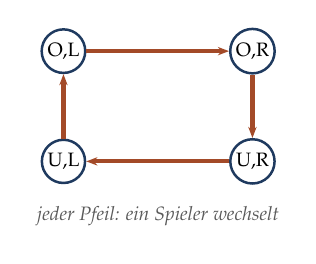
\begin{tikzpicture}[scale=1.0]
\node[knotenb] (OL) at (0,1.4) {O,L};
\node[knotenb] (OR) at (2.4,1.4) {O,R};
\node[knotenb] (UR) at (2.4,0) {U,R};
\node[knotenb] (UL) at (0,0) {U,L};
\draw[kanted, -{Stealth[length=4pt]}] (OL)--(OR);
\draw[kanted, -{Stealth[length=4pt]}] (OR)--(UR);
\draw[kanted, -{Stealth[length=4pt]}] (UR)--(UL);
\draw[kanted, -{Stealth[length=4pt]}] (UL)--(OL);
\node[font=\scriptsize\itshape, color=grau] at (1.2,-0.7) {jeder Pfeil: ein Spieler wechselt};
\end{tikzpicture}
\end{center}

\begin{center}
\begin{minipage}{0.9\textwidth}
\textbf{Kein Feld ist stabil --- immer will einer wechseln.}
\end{minipage}
\end{center}

\schritt{Schritt 3 --- Das gemischte Gleichgewicht}
\kursiv{Zeilenspieler gleichgültig:}
\[ 3q + 0(1-q) = 1q + 2(1-q) \]
\[ 3q = 2 - q \quad\Longrightarrow\quad 4q = 2 \quad\Longrightarrow\quad q = \tfrac12 \]

\kursiv{Spaltenspieler gleichgültig:}
\[ 1p + 3(1-p) = 2p + 0(1-p) \]
\[ 3 - 2p = 2p \quad\Longrightarrow\quad 4p = 3 \quad\Longrightarrow\quad p = \tfrac34 \]

\schritt{Schritt 4 --- Die Auszahlungen}
\kursiv{Zeilenspieler:} $3\cdot\tfrac12 = \tfrac32$.\\
\kursiv{Probe:} $1\cdot\tfrac12 + 2\cdot\tfrac12 = \tfrac32$ \checkmark

\kursiv{Spaltenspieler:} $1\cdot\tfrac34 + 3\cdot\tfrac14 = \tfrac34+\tfrac34 = \tfrac32$.\\
\kursiv{Probe:} $2\cdot\tfrac34 + 0 = \tfrac32$ \checkmark

\schritt{Schritt 5 --- Ist das ein Nullsummenspiel?}
\begin{center}
\renewcommand{\arraystretch}{1.46}
\begin{tabular}{@{}P{2.0cm}P{2.0cm}P{2.4cm}@{}}
\toprule
\textbf{Feld} & \textbf{Summe} & \\
\midrule
$(\text{O},\text{L})$ & $4$ & \\
$(\text{O},\text{R})$ & $2$ & \\
$(\text{U},\text{L})$ & $4$ & \\
$(\text{U},\text{R})$ & $2$ & \\
\bottomrule
\end{tabular}
\end{center}

\begin{center}
\begin{minipage}{0.9\textwidth}
\textbf{Nein --- die Summen sind verschieden.} Es ist ein echtes Nichtnullsummenspiel mit einem einzigen, gemischten Gleichgewicht.
\end{minipage}
\end{center}

\begin{center}
\begin{minipage}{0.88\textwidth}
\kursiv{Bemerkenswert ist, dass beide Felder mit Summe $4$ --- also mit höherem Gesamtertrag --- im Gleichgewicht nur mit Wahrscheinlichkeit $\tfrac34\cdot\tfrac12 + \tfrac14\cdot\tfrac12 = \tfrac12$ erreicht werden. \textbf{Es gibt keine Möglichkeit, das zu verbessern}, ohne dass einer der beiden einen Grund zum Abweichen bekommt.}
\end{minipage}
\end{center}
\end{aufgabe}

\begin{aufgabe}
\boxtitel{Aufgabe 4.3 --- Ein Nutzen aus Vorlieben}
Ein Chefarzt zieht eine sichere Verlegung ($V$) einer Notoperation vor, diese wiederum dem Abwarten ($A$). Bei einer Lotterie zwischen Notoperation und Abwarten ist er gleichgültig gegenüber der Verlegung, wenn die Notoperation mit $0{,}8$ eintritt. Konstruieren Sie eine Nutzenfunktion.

\loesung
\schritt{Schritt 1 --- Die Skala festlegen}
Nach Satz 4.1 ist der Nutzen bis auf eine positive affine Umrechnung bestimmt. Man darf also zwei Werte frei wählen.

\begin{center}
\renewcommand{\arraystretch}{1.48}
\begin{tabular}{@{}P{2.6cm}P{2.0cm}P{2.6cm}@{}}
\toprule
\textbf{Ergebnis} & \textbf{Nutzen} & \\
\midrule
Notoperation ($N$) & $1$ & bestes\\
Abwarten ($A$) & $0$ & schlechtestes\\
\bottomrule
\end{tabular}
\end{center}

\begin{center}
\begin{minipage}{0.86\textwidth}
\kursiv{Vorsicht bei der Anordnung: Genannt wurde $V$ vor $N$ vor $A$. Die Skala wird an den \kursiv{Extremen} verankert --- hier $V$ als bestes und $A$ als schlechtestes. Wir setzen sie also neu.}
\end{minipage}
\end{center}

\begin{center}
\renewcommand{\arraystretch}{1.48}
\begin{tabular}{@{}P{2.6cm}P{2.0cm}P{2.6cm}@{}}
\toprule
\textbf{Ergebnis} & \textbf{Nutzen} & \\
\midrule
Verlegung ($V$) & $1$ & bestes\\
Abwarten ($A$) & $0$ & schlechtestes\\
Notoperation ($N$) & $u$ & gesucht\\
\bottomrule
\end{tabular}
\end{center}

\schritt{Schritt 2 --- Die Angabe auswerten}
Die genannte Gleichgültigkeit lautet: $V$ ist genauso gut wie die Lotterie, die mit $0{,}8$ zu $N$ und mit $0{,}2$ zu $A$ führt.

\[ \Aus(V) = 0{,}8\,\Aus(N) + 0{,}2\,\Aus(A) \]
\[ 1 = 0{,}8\,u + 0 \quad\Longrightarrow\quad u = \tfrac{1}{0{,}8} = 1{,}25 \]

\schritt{Schritt 3 --- Der Widerspruch}
\begin{center}
\begin{minipage}{0.9\textwidth}
\textbf{Es käme $\Aus(N) = 1{,}25 > 1 = \Aus(V)$ heraus --- im Widerspruch dazu, dass $V$ vorgezogen wird.}
\end{minipage}
\end{center}

\begin{center}
\begin{minipage}{0.88\textwidth}
\kursiv{Die Angaben sind unvereinbar. Eine Lotterie zwischen $N$ und $A$ kann nie besser sein als $N$ --- und da $V$ besser als $N$ ist, kann keine solche Lotterie $V$ erreichen. \textbf{Die Stetigkeitsforderung verlangt die Gleichgültigkeit für ein $\lambda$ zwischen den \kursiv{umschließenden} Ergebnissen}, nicht zwischen zwei schlechteren.}
\end{minipage}
\end{center}

\schritt{Schritt 4 --- Die richtige Frage}
Man fragt nach der Lotterie zwischen dem besten und dem schlechtesten Ergebnis:

\kursiv{\enquote{Ab welcher Erfolgswahrscheinlichkeit $\lambda$ einer Lotterie zwischen Verlegung und Abwarten würden Sie diese der Notoperation vorziehen?}}

Antworte der Chefarzt mit $\lambda = 0{,}8$, so folgt
\[ \Aus(N) = 0{,}8\cdot1 + 0{,}2\cdot0 = 0{,}8 \]

\begin{center}
\renewcommand{\arraystretch}{1.48}
\begin{tabular}{@{}P{2.6cm}P{2.0cm}P{2.6cm}@{}}
\toprule
\textbf{Ergebnis} & \textbf{Nutzen} & \\
\midrule
Verlegung & $1{,}0$ & \\
Notoperation & $0{,}8$ & \\
Abwarten & $0{,}0$ & \\
\bottomrule
\end{tabular}
\end{center}

\schritt{Schritt 5 --- Die Probe auf Konsistenz}
\[ \Aus(V) = 1{,}0 \ >\ \Aus(N) = 0{,}8 \ >\ \Aus(A) = 0{,}0 \quad \checkmark \]

\schritt{Schritt 6 --- Die Eindeutigkeit prüfen}
Eine andere Skala, etwa $\Aus(V) = 10$ und $\Aus(A) = 2$, ergäbe
\[ \Aus(N) = 0{,}8\cdot10 + 0{,}2\cdot2 = 8{,}4 \]

\kursiv{Umrechnung:} $8{,}4 = 8\cdot0{,}8 + 2$ --- also genau $\alpha\,\Aus + \beta$ mit $\alpha=8$, $\beta=2$. \checkmark

\begin{center}
\begin{minipage}{0.88\textwidth}
\kursiv{Die Verhältnisse von Nutzen\kursiv{differenzen} bleiben erhalten, die Verhältnisse der Nutzen selbst nicht. \textbf{Es ist daher sinnlos zu sagen, die Verlegung sei \enquote{$1{,}25$-mal so gut} wie die Notoperation} --- in der zweiten Skala wäre es der Faktor $1{,}19$. Sinnvoll ist nur: Der Abstand zwischen Verlegung und Notoperation beträgt ein Viertel des Abstands zwischen Notoperation und Abwarten.}
\end{minipage}
\end{center}

\kursiv{Probe:} $\frac{1{,}0-0{,}8}{0{,}8-0{,}0} = \frac{0{,}2}{0{,}8} = \frac14$ und $\frac{10-8{,}4}{8{,}4-2} = \frac{1{,}6}{6{,}4} = \frac14$ \checkmark
\end{aufgabe}

\begin{geschichte}
\boxtitelg{Siebenundzwanzig Seiten und ein kühler Empfang}
\Person{John Nash} (1928--2015) kam 1948 mit zwanzig Jahren nach Princeton. Sein Empfehlungsschreiben bestand aus einem Satz: \enquote{Dieser Mann ist ein Genie.}

\begin{center}
\begin{minipage}{0.9\textwidth}
\kursiv{Seine Dissertation von 1950 umfasst siebenundzwanzig Seiten und enthält die Definition des Gleichgewichts, den Existenzbeweis und zwei Beispiele. Das Literaturverzeichnis führt zwei Titel auf, einer davon von Neumann und Morgenstern.}
\end{minipage}
\end{center}

\schritt{Das Gespräch}
Nash stellte seine Idee von Neumann vor. Dieser hörte kurz zu und sagte, das sei trivial --- ein Fixpunktsatz.

\begin{center}
\begin{minipage}{0.9\textwidth}
\kursiv{Technisch hatte er recht: Der Beweis benutzt denselben Satz von Brouwer, den von Neumann 1928 verwendet hatte, und ist kürzer als dessen eigener. \textbf{Begrifflich lag er falsch} --- und zwar deutlich. Der Gleichgewichtsbegriff hat die Wirtschaftswissenschaft umgestaltet, während von Neumanns Koalitionstheorie aus demselben Buch heute vergleichsweise wenig benutzt wird.}
\end{minipage}
\end{center}

\schritt{Warum die Ablehnung}
Von Neumann hielt den nichtkooperativen Ansatz für zu eng: Spieler, die nicht verhandeln dürfen, seien eine unrealistische Vereinfachung.

\begin{center}
\begin{minipage}{0.9\textwidth}
\kursiv{Auch dieser Einwand ist ernstzunehmen und kehrt in Kapitel~14 wieder. \textbf{Die Geschichte gab Nash recht, ohne von Neumann unrecht zu geben} --- beide Zugänge bestehen nebeneinander, nur hat der eine sich als anschlussfähiger erwiesen.}
\end{minipage}
\end{center}

\schritt{Die späte Anerkennung}
Nash erkrankte Ende der 1950er Jahre an einer Schizophrenie und war jahrzehntelang arbeitsunfähig.

\begin{center}
\begin{minipage}{0.9\textwidth}
\kursiv{In den 1980er Jahren besserte sich sein Zustand; 1994 erhielt er gemeinsam mit \Person{Harsanyi} und \Person{Selten} den Wirtschaftsnobelpreis. \textbf{Das Nobelkomitee hatte lange gezögert} --- nicht wegen der Leistung, sondern wegen der Frage, ob er die Auszeichnung würde entgegennehmen können. Nash starb 2015 bei einem Verkehrsunfall, wenige Tage nach der Verleihung des Abelpreises für eine ganz andere Arbeit: seine Ergebnisse über partielle Differentialgleichungen, die er selbst für gewichtiger hielt.}
\end{minipage}
\end{center}
\end{geschichte}

\begin{forschung}
\boxtitelp{Was am Gleichgewichtsbegriff gearbeitet wird}
\begin{center}
{\small
\renewcommand{\arraystretch}{1.45}
\begin{tabular}{@{}P{2.8cm}P{5.4cm}@{}}
\toprule
\textbf{Auswahl} & Welches Gleichgewicht wird erreicht, wenn es mehrere gibt? Kapitel~8 und 10.\\
\textbf{Verfeinerungen} & Zusatzbedingungen, die unplausible Gleichgewichte ausschließen.\\
\textbf{Lernen} & Ob wiederholtes Spielen zum Gleichgewicht führt --- und zu welchem.\\
\bottomrule
\end{tabular}}
\end{center}

\schritt{Zur zweiten Zeile}
\Person{Reinhard Selten} führte 1965 die Teilspielperfektheit ein, 1975 die zitternde Hand.

\begin{center}
\begin{minipage}{0.88\textwidth}
\kursiv{Beide schließen Gleichgewichte aus, die auf unglaubwürdigen Drohungen beruhen oder gegen kleine Fehler nicht robust sind. \textbf{Der Ansatz hat einen Nachteil, den Selten selbst benannte}: Die Zahl der Verfeinerungen wuchs rasch, ohne dass sich eine als die richtige erwies. Kapitel~7 behandelt die wichtigste davon.}
\end{minipage}
\end{center}

\schritt{Zur dritten Zeile}
Verschiedene Lernverfahren führen zu verschiedenen Ergebnissen.

\begin{center}
\begin{minipage}{0.88\textwidth}
\kursiv{Bei Nullsummenspielen konvergieren die meisten Verfahren gegen das Gleichgewicht --- Kapitel~3 nannte ein Beispiel. \textbf{Bei Nichtnullsummenspielen gilt das nicht}: Es gibt Spiele, in denen naheliegende Lernverfahren nachweislich nie konvergieren, sondern dauerhaft kreisen. Das ist kein Randphänomen und wird in Kapitel~10 an der Replikatordynamik sichtbar.}
\end{minipage}
\end{center}
\end{forschung}

\begin{merksatz}
\boxtitel{Was Sie jetzt können}
\begin{center}
\renewcommand{\arraystretch}{1.5}
\begin{tabular}{@{}P{3.0cm}P{5.6cm}@{}}
\toprule
\textbf{Satz 4.1} & wann man mitteln darf\\
\textbf{Definition 4.3} & niemand gewinnt durch Abweichen\\
\textbf{Der Leitfall} & zwei reine, ein gemischtes\\
\textbf{Gemischt rechnen} & den anderen gleichgültig machen\\
\textbf{Der Verlust} & kein Wert, keine Garantie, kein Rat\\
\bottomrule
\end{tabular}
\end{center}

\begin{center}
\begin{minipage}{0.88\textwidth}
\kursiv{Im nächsten Kapitel betrachten wir vier Spiele mit je zwei Strategien. Sie sind vollständig durchgerechnet und in wenigen Zeilen beschrieben --- und sie haben mehr Literatur erzeugt als der Rest dieses Bandes zusammen.}
\end{minipage}
\end{center}
\end{merksatz}

\chapter{Drei Spiele, die alles erklären}

\section{Dieselbe Form, verschiedene Welten}

\begin{merksatz}
\boxtitel{Der gemeinsame Rahmen}
Alle drei Spiele dieses Kapitels sind symmetrisch, haben zwei Strategien je Spieler und werden durch vier Zahlen beschrieben.

\begin{center}
{\small
\renewcommand{\arraystretch}{1.6}
\begin{tabular}{@{}P{2.4cm}P{2.4cm}P{2.4cm}@{}}
\toprule
& \textbf{mitziehen} & \textbf{ausscheren}\\
\midrule
\textbf{mitziehen} & $(R,\ R)$ & $(S,\ T)$\\
\textbf{ausscheren} & $(T,\ S)$ & $(P,\ P)$\\
\bottomrule
\end{tabular}}
\end{center}

\begin{center}
{\small
\renewcommand{\arraystretch}{1.48}
\begin{tabular}{@{}P{1.4cm}P{3.0cm}P{3.6cm}@{}}
\toprule
$R$ & \kursiv{Reward} & beide ziehen mit\\
$T$ & \kursiv{Temptation} & allein ausscheren\\
$S$ & \kursiv{Sucker} & allein mitziehen\\
$P$ & \kursiv{Punishment} & beide scheren aus\\
\bottomrule
\end{tabular}}
\end{center}

\begin{center}
\begin{minipage}{0.9\textwidth}
\textbf{Allein die \kursiv{Reihenfolge} dieser vier Zahlen entscheidet, welches Spiel vorliegt --- und die drei Anordnungen führen zu grundverschiedenen Empfehlungen.}
\end{minipage}
\end{center}

\begin{center}
\begin{minipage}{0.88\textwidth}
\kursiv{Es kommt nicht auf die Zahlen an, sondern auf ihre Ordnung. \textbf{Zwei Spiele mit völlig verschiedenen Zahlen sind dasselbe Spiel}, wenn die Reihenfolge übereinstimmt --- das folgt aus der Eindeutigkeit des Nutzens bis auf affine Umrechnung, Satz 4.1. Und umgekehrt: Zwei Spiele mit fast gleichen Zahlen sind völlig verschieden, wenn eine Vertauschung stattgefunden hat.}
\end{minipage}
\end{center}
\end{merksatz}

\section{Das Gefangenendilemma}

\begin{merksatz}
\boxtitel{Der Leitfall: Reserveantibiotika}
Beide Häuser können ein Reserveantibiotikum großzügig einsetzen oder zurückhalten. Großzügiger Einsatz nützt den eigenen Patienten unmittelbar; die entstehenden Resistenzen tragen beide.

\begin{center}
{\small
\renewcommand{\arraystretch}{1.6}
\begin{tabular}{@{}P{2.6cm}P{2.4cm}P{2.4cm}@{}}
\toprule
\textbf{Klinikum} & \textbf{M.: zurück} & \textbf{M.: frei}\\
\midrule
zurückhalten & $(3,\ 3)$ & $(0,\ 5)$\\
frei einsetzen & $(5,\ 0)$ & $(1,\ 1)$\\
\bottomrule
\end{tabular}}
\end{center}

\[ T = 5 \ >\ R = 3 \ >\ P = 1 \ >\ S = 0 \]

\schritt{Die Lösung}
\kursiv{Für das Klinikum:} Hält das Marienhospital zurück, so bringt freier Einsatz $5$ statt $3$. Setzt es frei ein, so bringt freier Einsatz $1$ statt $0$.

\begin{center}
\begin{minipage}{0.9\textwidth}
\textbf{Freier Einsatz dominiert strikt.} Beide Häuser wählen ihn, und beide erhalten $1$.
\end{minipage}
\end{center}

\schritt{Der Vergleich}
\begin{center}
{\small
\renewcommand{\arraystretch}{1.5}
\begin{tabular}{@{}P{2.8cm}P{2.0cm}P{2.0cm}P{1.6cm}@{}}
\toprule
& \textbf{K} & \textbf{M} & \\
\midrule
Gleichgewicht & $1$ & $1$ & \\
beide zurück & $\mathbf{3}$ & $\mathbf{3}$ & \textcolor{gruen}{besser}\\
\bottomrule
\end{tabular}}
\end{center}

\begin{center}
\begin{minipage}{0.9\textwidth}
\textbf{Das einzige Gleichgewicht ist für beide Spieler schlechter als eine erreichbare Alternative.}
\end{minipage}
\end{center}

\begin{center}
\begin{minipage}{0.88\textwidth}
\kursiv{Das ist die schärfste Fassung der dritten Warnung aus dem Vorwort. \textbf{Hier fallen Gleichgewicht und Optimum nicht nur auseinander --- sie widersprechen sich.} Und die Argumentation, die dorthin führt, ist nicht zu entkräften: Dominanz braucht keinerlei Annahme über das Verhalten des anderen.}
\end{minipage}
\end{center}
\end{merksatz}

\begin{warnung}
\boxtitelr{Was daraus nicht folgt}
\begin{center}
{\small
\renewcommand{\arraystretch}{1.52}
\begin{tabular}{@{}P{2.4cm}P{6.2cm}@{}}
\toprule
\textbf{Nicht:} & \enquote{Zusammenarbeit lohnt sich nicht.} Sie lohnt sich sehr --- sie ist nur einseitig nicht durchsetzbar.\\
\textbf{Nicht:} & \enquote{Menschen kooperieren nicht.} Sie tun es häufig, und die Kapitel~7 bis 10 erklären, warum.\\
\textbf{Nicht:} & \enquote{So ist die Welt.} Es ist ein Modell mit einer Runde, ohne Absprache, ohne Vorgeschichte und ohne Aufsicht.\\
\bottomrule
\end{tabular}}
\end{center}

\begin{center}
\begin{minipage}{0.9\textwidth}
\textbf{Das Gefangenendilemma ist keine Aussage über Menschen, sondern über eine Anreizlage.}
\end{minipage}
\end{center}

\begin{center}
\begin{minipage}{0.88\textwidth}
\kursiv{Und es ist zugleich eine Handlungsanweisung --- allerdings nicht an die Spieler, sondern an den, der die Regeln setzt. \textbf{Wer das Ergebnis ändern will, muss die Auszahlungen ändern}, nicht die Spieler ermahnen. Im Leitfall geschieht genau das: Verordnungen zur Antibiotikaverschreibung und verpflichtende Resistenzmeldungen verändern $T$ und $P$, bis die Dominanz kippt. Kapitel~11 behandelt diesen Zugang systematisch.}
\end{minipage}
\end{center}
\end{warnung}

\section{Das Feigheitsspiel}

\begin{merksatz}
\boxtitel{Der Leitfall: Ausbau einer Spezialabteilung}
Beide Häuser erwägen den Aufbau einer teuren Spezialabteilung. Wer allein ausbaut, gewinnt die Zuweisungen. Bauen beide aus, so tragen beide die Kosten bei halber Auslastung.

\begin{center}
{\small
\renewcommand{\arraystretch}{1.6}
\begin{tabular}{@{}P{2.6cm}P{2.4cm}P{2.4cm}@{}}
\toprule
\textbf{Klinikum} & \textbf{M.: verzicht} & \textbf{M.: baut}\\
\midrule
verzichten & $(3,\ 3)$ & $(2,\ 5)$\\
ausbauen & $(5,\ 2)$ & $(1,\ 1)$\\
\bottomrule
\end{tabular}}
\end{center}

\[ T = 5 \ >\ R = 3 \ >\ S = 2 \ >\ P = 1 \]

\begin{center}
\begin{minipage}{0.9\textwidth}
\textbf{Der einzige Unterschied zum Gefangenendilemma: $S$ und $P$ sind vertauscht.} Beidseitiges Ausscheren ist nun das schlechteste Ergebnis.
\end{minipage}
\end{center}

\schritt{Die Folgen}
\begin{center}
{\small
\renewcommand{\arraystretch}{1.5}
\begin{tabular}{@{}P{2.4cm}P{6.2cm}@{}}
\toprule
\textbf{Keine Dominanz} & Gegen Verzicht ist Ausbau besser ($5>3$), gegen Ausbau ist Verzicht besser ($2>1$).\\
\textbf{Zwei Gleichgewichte} & $(\text{bauen},\text{verzichten})$ und $(\text{verzichten},\text{bauen})$.\\
\bottomrule
\end{tabular}}
\end{center}

\schritt{Das gemischte Gleichgewicht}
\[ q\cdot3 + (1-q)\cdot2 = q\cdot5 + (1-q)\cdot1 \]
\[ 2+q = 1+4q \quad\Longrightarrow\quad 3q = 1 \quad\Longrightarrow\quad q = \tfrac13 \]

\kursiv{Auszahlung:} $\tfrac13\cdot3 + \tfrac23\cdot2 = 1+\tfrac43 = \tfrac73 \approx 2{,}33$\\
\kursiv{Probe:} $\tfrac13\cdot5 + \tfrac23\cdot1 = \tfrac53+\tfrac23 = \tfrac73$ \checkmark

\schritt{Die entscheidende Zahl}
Beide bauen aus mit Wahrscheinlichkeit
\[ \left(\tfrac23\right)^{2} = \tfrac49 \approx 44\,\% . \]

\begin{center}
\begin{minipage}{0.9\textwidth}
\textbf{In fast der Hälfte der Fälle tritt das schlechteste Ergebnis ein.}
\end{minipage}
\end{center}

\begin{center}
\begin{minipage}{0.88\textwidth}
\kursiv{Und zwar ohne dass jemand etwas falsch macht. \textbf{Das Feigheitsspiel bestraft Entschlossenheit auf beiden Seiten}, und deshalb lohnt sich hier, was im Gefangenendilemma wirkungslos wäre: sich glaubhaft festzulegen. Wer zuerst und unwiderruflich baut, gewinnt --- Kapitel~7 zeigt, wie sich das formal fassen lässt und warum es ein anderes Spiel erzeugt.}
\end{minipage}
\end{center}
\end{merksatz}

\section{Die Hirschjagd}

\begin{merksatz}
\boxtitel{Der Leitfall: ein gemeinsames Notfallzentrum}
Beide Häuser können in ein gemeinsames Zentrum investieren oder ihre eigene Notaufnahme weiterbetreiben. Das Zentrum lohnt sich nur, wenn beide mitziehen.

\begin{center}
{\small
\renewcommand{\arraystretch}{1.6}
\begin{tabular}{@{}P{2.6cm}P{2.4cm}P{2.4cm}@{}}
\toprule
\textbf{Klinikum} & \textbf{M.: gemeins.} & \textbf{M.: allein}\\
\midrule
gemeinsam & $(4,\ 4)$ & $(0,\ 3)$\\
allein & $(3,\ 0)$ & $(3,\ 3)$\\
\bottomrule
\end{tabular}}
\end{center}

\[ R = 4 \ >\ T = 3 = P \ >\ S = 0 \]

\schritt{Die beiden Gleichgewichte}
\begin{center}
{\small
\renewcommand{\arraystretch}{1.5}
\begin{tabular}{@{}P{2.6cm}P{2.0cm}P{3.0cm}@{}}
\toprule
\textbf{Gleichgewicht} & \textbf{Auszahlung} & \\
\midrule
beide gemeinsam & $(4,4)$ & \textcolor{gruen}{auszahlungsbesser}\\
beide allein & $(3,3)$ & \textcolor{akzent}{risikoärmer}\\
\bottomrule
\end{tabular}}
\end{center}

\begin{center}
\begin{minipage}{0.9\textwidth}
\textbf{Hier stimmen die Interessen überein --- und trotzdem ist die bessere Lösung nicht gesichert.}
\end{minipage}
\end{center}

\schritt{Warum}
\[ q\cdot4 + (1-q)\cdot0 = q\cdot3 + (1-q)\cdot3 \]
\[ 4q = 3 \quad\Longrightarrow\quad q = \tfrac34 \]

\begin{center}
\begin{minipage}{0.9\textwidth}
\textbf{Man muss zu mindestens $75$ Prozent darauf vertrauen, dass der andere mitzieht, damit sich das Mitziehen lohnt.}
\end{minipage}
\end{center}

\begin{center}
\begin{minipage}{0.88\textwidth}
\kursiv{Das ist eine bemerkenswert hohe Schwelle. Das Alleingehen bringt $3$ --- unabhängig davon, was der andere tut. Das Mitziehen bringt $4$, aber nur bei Gegenseitigkeit, sonst $0$. \textbf{Das Risiko ist einseitig}, und wer es scheut, wählt den sicheren Weg. Man nennt $(\text{allein},\text{allein})$ deshalb \Begriff{risikodominant} und $(\text{gemeinsam},\text{gemeinsam})$ \Begriff{auszahlungsdominant}.}
\end{minipage}
\end{center}

\schritt{Der Unterschied zum Gefangenendilemma}
\begin{center}
{\small
\renewcommand{\arraystretch}{1.5}
\begin{tabular}{@{}P{2.4cm}P{6.2cm}@{}}
\toprule
\textbf{Dilemma} & Mitziehen ist \kursiv{nie} eine beste Antwort. Das Problem sind die Anreize.\\
\textbf{Hirschjagd} & Mitziehen ist eine beste Antwort --- wenn der andere es tut. Das Problem ist das Vertrauen.\\
\bottomrule
\end{tabular}}
\end{center}

\begin{center}
\begin{minipage}{0.88\textwidth}
\kursiv{Diese Unterscheidung ist für die Praxis wesentlich: \textbf{Ein Dilemma löst man durch veränderte Anreize, eine Hirschjagd durch Kommunikation.} Eine bindende Absprache genügt hier bereits --- sie muss nicht einmal durchsetzbar sein, denn niemand hat einen Grund, sie zu brechen. Im Gefangenendilemma wäre dieselbe Absprache wertlos.}
\end{minipage}
\end{center}
\end{merksatz}

\section{Die Systematik}

\begin{merksatz}
\boxtitel{Die drei Anordnungen im Vergleich}
\begin{center}
{\small
\renewcommand{\arraystretch}{1.52}
\begin{tabular}{@{}P{2.0cm}P{2.4cm}P{1.6cm}P{2.6cm}@{}}
\toprule
\textbf{Spiel} & \textbf{Ordnung} & \textbf{GG} & \textbf{Problem}\\
\midrule
Dilemma & $T>R>P>S$ & $1$ & Anreize\\
Feigheit & $T>R>S>P$ & $3$ & Entschlossen\-heit\\
Hirschjagd & $R>T\ge P>S$ & $3$ & Vertrauen\\
\bottomrule
\end{tabular}}
\end{center}

\begin{center}
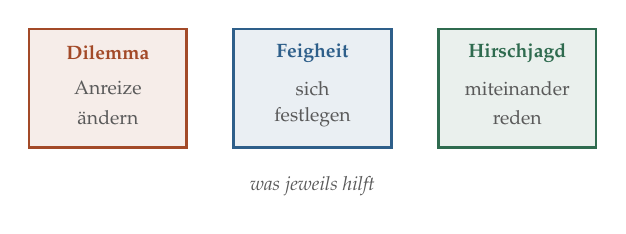
\begin{tikzpicture}[scale=1.0]
\foreach \x/\lab/\col in {0/Dilemma/akzent, 2.6/Feigheit/mittel, 5.2/Hirschjagd/gruen} {
  \draw[\col, line width=1.0pt, fill=\col!10] (\x,0) rectangle ++(2.0,1.5);
  \node[font=\scriptsize\bfseries, color=\col] at (\x+1.0,1.2) {\lab};
}
\node[font=\scriptsize, color=grau] at (1.0,0.75) {Anreize};
\node[font=\scriptsize, color=grau] at (1.0,0.38) {ändern};
\node[font=\scriptsize, color=grau] at (3.6,0.75) {sich};
\node[font=\scriptsize, color=grau] at (3.6,0.38) {festlegen};
\node[font=\scriptsize, color=grau] at (6.2,0.75) {miteinander};
\node[font=\scriptsize, color=grau] at (6.2,0.38) {reden};
\node[font=\scriptsize\itshape, color=grau] at (3.6,-0.5) {was jeweils hilft};
\end{tikzpicture}
\end{center}

\begin{center}
\begin{minipage}{0.88\textwidth}
\kursiv{Diese Tabelle ist das eigentliche Ergebnis des Kapitels. \textbf{Die richtige Maßnahme hängt davon ab, welches Spiel vorliegt} --- und wer das falsch bestimmt, wendet ein wirkungsloses Mittel an. Miteinander reden hilft bei der Hirschjagd und ist im Dilemma vergeblich; veränderte Anreize helfen im Dilemma und sind bei der Hirschjagd unnötiger Aufwand.}
\end{minipage}
\end{center}
\end{merksatz}

\begin{warnung}
\boxtitelr{Die Einordnung ist heikel}
Zwischen Dilemma und Feigheitsspiel liegt nur die Vertauschung von $S$ und $P$.

\begin{center}
{\small
\renewcommand{\arraystretch}{1.5}
\begin{tabular}{@{}P{2.8cm}P{5.6cm}@{}}
\toprule
\textbf{Die Frage} & Ist beidseitiges Ausscheren schlimmer oder besser als einseitiges Mitziehen?\\
\bottomrule
\end{tabular}}
\end{center}

\begin{center}
\begin{minipage}{0.9\textwidth}
\textbf{Von der Antwort hängt ab, ob es ein Gleichgewicht gibt oder drei --- und ob Reden hilft.}
\end{minipage}
\end{center}

\begin{center}
\begin{minipage}{0.88\textwidth}
\kursiv{Im Leitfall der Reserveantibiotika: Ist es schlimmer, wenn beide Häuser großzügig verschreiben ($P$), oder wenn man selbst zurückhält, während der andere verschreibt ($S$)? \textbf{Die Antwort hängt davon ab, wie weit Resistenzen zwischen den Häusern wandern.} Bleiben sie lokal, so ist $S$ erträglich und es liegt ein Dilemma vor. Wandern sie frei, so trägt man die Resistenzen ohnehin mit und hat nur den eigenen Nutzen verloren --- dann ist $S$ sehr schlecht, und es bleibt beim Dilemma. Eine Verschiebung zum Feigheitsspiel träte erst ein, wenn beidseitiger Vollgebrauch eine Katastrophe wäre, die einseitigen Verzicht lohnend macht.}
\end{minipage}
\end{center}

\schritt{Die Lehre}
\begin{center}
\begin{minipage}{0.88\textwidth}
\kursiv{\textbf{Die Modellwahl entscheidet die Empfehlung, und sie beruht auf einer Schätzung.} Das ist die erste Warnung des Vorworts, hier an einem Fall, in dem eine einzige vertauschte Ungleichung die Handlungsanweisung umkehrt. Wer spieltheoretisch argumentiert, sollte die Ordnung der vier Zahlen begründen können --- und die Empfindlichkeit prüfen, wie in Aufgabe 1.3.}
\end{minipage}
\end{center}
\end{warnung}

\section{Übungsaufgaben}

\begin{aufgabe}
\boxtitel{Aufgabe 5.1 --- Wann kippt die Dominanz?}
Im Leitfall der Reserveantibiotika führt eine Meldepflicht dazu, dass freier Einsatz mit einem Abschlag $k$ belegt wird. Ab welchem $k$ verschwindet das Dilemma?

\loesung
\schritt{Schritt 1 --- Die veränderte Matrix}
Der Abschlag trifft nur denjenigen, der frei einsetzt:
\begin{center}
{\small
\renewcommand{\arraystretch}{1.6}
\begin{tabular}{@{}P{2.4cm}P{2.6cm}P{2.6cm}@{}}
\toprule
& \textbf{zurück} & \textbf{frei}\\
\midrule
\textbf{zurück} & $(3,\ 3)$ & $(0,\ 5-k)$\\
\textbf{frei} & $(5-k,\ 0)$ & $(1-k,\ 1-k)$\\
\bottomrule
\end{tabular}}
\end{center}

\schritt{Schritt 2 --- Wann dominiert freier Einsatz nicht mehr?}
Zwei Vergleiche müssen beide gelten, damit freier Einsatz dominiert:
\begin{center}
{\small
\renewcommand{\arraystretch}{1.5}
\begin{tabular}{@{}P{2.8cm}P{3.0cm}P{2.4cm}@{}}
\toprule
\textbf{Gegner hält zurück} & $5-k > 3$ & $k < 2$\\
\textbf{Gegner setzt frei} & $1-k > 0$ & $k < 1$\\
\bottomrule
\end{tabular}}
\end{center}

\schritt{Schritt 3 --- Die Schwellen}
\begin{center}
{\small
\renewcommand{\arraystretch}{1.5}
\begin{tabular}{@{}P{1.8cm}P{3.4cm}P{2.6cm}@{}}
\toprule
$k$ & \textbf{Lage} & \textbf{Gleichgewicht}\\
\midrule
$k<1$ & Dominanz bleibt & $(\text{frei},\text{frei})$\\
$1<k<2$ & keine Dominanz & \textcolor{mittel}{Hirschjagd}\\
$k>2$ & Zurückhalten dominiert & $(\text{zurück},\text{zurück})$\\
\bottomrule
\end{tabular}}
\end{center}

\schritt{Schritt 4 --- Der mittlere Bereich genauer}
Bei $k = 1{,}5$:
\begin{center}
{\small
\renewcommand{\arraystretch}{1.6}
\begin{tabular}{@{}P{2.2cm}P{2.4cm}P{2.4cm}@{}}
\toprule
& \textbf{zurück} & \textbf{frei}\\
\midrule
\textbf{zurück} & $(3,\ 3)$ & $(0,\ 3{,}5)$\\
\textbf{frei} & $(3{,}5,\ 0)$ & $(-0{,}5,\ -0{,}5)$\\
\bottomrule
\end{tabular}}
\end{center}

\kursiv{Reine Gleichgewichte:}
\begin{center}
\renewcommand{\arraystretch}{1.48}
\begin{tabular}{@{}P{3.4cm}P{2.6cm}P{1.4cm}@{}}
\toprule
\textbf{Feld} & \textbf{Abweichen bringt} & \\
\midrule
$(\text{zurück},\text{zurück})$ & $3 \to 3{,}5$ & \textcolor{akzent}{kein GG}\\
$(\text{frei},\text{frei})$ & $-0{,}5 \to 0$ & \textcolor{akzent}{kein GG}\\
$(\text{frei},\text{zurück})$ & $3{,}5\to3$; $0\to-0{,}5$ & \textcolor{gruen}{GG}\\
\bottomrule
\end{tabular}
\end{center}

\begin{center}
\begin{minipage}{0.9\textwidth}
\textbf{Bei mittlerem Abschlag entsteht ein Feigheitsspiel, kein Dilemma und keine Lösung.}
\end{minipage}
\end{center}

\begin{center}
\begin{minipage}{0.88\textwidth}
\kursiv{Man beachte die Reihenfolge: $T = 3{,}5 > R = 3 > S = 0 > P = -0{,}5$ --- das ist genau die Anordnung des Feigheitsspiels. \textbf{Eine halbherzige Maßnahme verwandelt das Dilemma nicht in Zusammenarbeit, sondern in einen Wettbewerb darum, wer zuerst ausschert.} Das ist eine Warnung an jeden, der Anreize nur ein bisschen verschiebt.}
\end{minipage}
\end{center}

\schritt{Schritt 5 --- Die Antwort}
\[ k > 2 \]

\begin{center}
\begin{minipage}{0.88\textwidth}
\kursiv{Der Abschlag muss also die gesamte Versuchung $T - R = 2$ aufzehren --- nicht nur einen Teil. \textbf{Das ist die allgemeine Regel: Eine Maßnahme gegen ein Dilemma muss mindestens $T-R$ kosten}, sonst bleibt die Dominanz bestehen oder es entsteht Schlimmeres.}
\end{minipage}
\end{center}
\end{aufgabe}

\begin{aufgabe}
\boxtitel{Aufgabe 5.2 --- Das Feigheitsspiel und die Festlegung}
Im Ausbauspiel legt sich das Klinikum öffentlich und unwiderruflich auf den Ausbau fest, bevor das Marienhospital entscheidet. Was ändert sich?

\loesung
\schritt{Schritt 1 --- Das ursprüngliche Spiel}
\begin{center}
{\small
\renewcommand{\arraystretch}{1.5}
\begin{tabular}{@{}P{2.8cm}P{2.2cm}P{2.4cm}@{}}
\toprule
\textbf{Gleichgewicht} & \textbf{K} & \textbf{M}\\
\midrule
$(\text{bauen},\text{verzicht})$ & $5$ & $2$\\
$(\text{verzicht},\text{bauen})$ & $2$ & $5$\\
gemischt & $2{,}33$ & $2{,}33$\\
\bottomrule
\end{tabular}}
\end{center}

\schritt{Schritt 2 --- Nach der Festlegung}
Das Marienhospital steht vor einer einfachen Wahl:
\begin{center}
\renewcommand{\arraystretch}{1.48}
\begin{tabular}{@{}P{2.4cm}P{2.0cm}P{2.6cm}@{}}
\toprule
\textbf{M wählt} & \textbf{erhält} & \\
\midrule
verzichten & $2$ & \textcolor{gruen}{besser}\\
bauen & $1$ & \\
\bottomrule
\end{tabular}
\end{center}

\begin{center}
\begin{minipage}{0.9\textwidth}
\textbf{Das Marienhospital verzichtet, das Klinikum erhält $5$.}
\end{minipage}
\end{center}

\schritt{Schritt 3 --- Der Gewinn}
\[ 5 - 2{,}33 = 2{,}67 \]

\begin{center}
\begin{minipage}{0.88\textwidth}
\kursiv{Verglichen mit dem gemischten Gleichgewicht gewinnt das Klinikum erheblich. \textbf{Und das Marienhospital verliert nur wenig} --- von $2{,}33$ auf $2$ --- weil das gemischte Gleichgewicht ohnehin schlecht war. Die Festlegung schafft Wert, und zwar überwiegend für den, der sie vornimmt.}
\end{minipage}
\end{center}

\schritt{Schritt 4 --- Warum \kursiv{unwiderruflich} das Entscheidende ist}
Wäre die Festlegung widerrufbar, so wäre sie wertlos.

\begin{center}
\begin{minipage}{0.88\textwidth}
\kursiv{Denn das Marienhospital könnte seinerseits bauen und darauf setzen, dass das Klinikum einlenkt --- und das Klinikum \kursiv{würde} einlenken, denn $2 > 1$. \textbf{Die Drohung ist nur glaubwürdig, wenn ihre Ausführung nicht mehr in der Hand des Drohenden liegt.} Genau das ist der Begriff der Teilspielperfektheit aus Kapitel~7.}
\end{minipage}
\end{center}

\schritt{Schritt 5 --- Wie man sich festlegt}
\begin{center}
{\small
\renewcommand{\arraystretch}{1.5}
\begin{tabular}{@{}P{2.8cm}P{5.8cm}@{}}
\toprule
\textbf{Verträge} & Baugenehmigung, Bestellungen, Personalverträge mit Konventionalstrafen.\\
\textbf{Öffentlichkeit} & Eine angekündigte Kehrtwende kostet Ansehen.\\
\textbf{Unumkehrbares} & Der ausgehobene Bauplatz ist das stärkste Argument.\\
\bottomrule
\end{tabular}}
\end{center}

\begin{center}
\begin{minipage}{0.88\textwidth}
\kursiv{\textbf{Alle drei Mittel verkleinern den eigenen Handlungsspielraum --- und genau darin liegt ihr Wert.} Das ist eine der wenigen Stellen, an denen die Theorie einer verbreiteten Intuition offen widerspricht: Mehr Möglichkeiten zu haben, ist nicht immer besser. \Person{Thomas Schelling} hat diesen Gedanken 1960 ausgearbeitet und dafür 2005 den Nobelpreis erhalten.}
\end{minipage}
\end{center}

\schritt{Schritt 6 --- Der Vorbehalt}
Legen sich \kursiv{beide} fest, so tritt $(1,1)$ ein.

\begin{center}
\begin{minipage}{0.86\textwidth}
\kursiv{Das Wettrennen um die frühere Festlegung ist selbst ein Spiel --- und es hat dieselbe Struktur wie das ursprüngliche. \textbf{Die Lösung durch Festlegung verschiebt das Problem eine Ebene nach oben}, statt es aufzulösen.}
\end{minipage}
\end{center}
\end{aufgabe}

\begin{aufgabe}
\boxtitel{Aufgabe 5.3 --- Risiko gegen Ertrag}
Bestimmen Sie in der Hirschjagd, wie sich die Vertrauensschwelle ändert, wenn der Alleingang statt $3$ nur $2$ einbringt.

\loesung
\schritt{Schritt 1 --- Die neue Matrix}
\begin{center}
{\small
\renewcommand{\arraystretch}{1.6}
\begin{tabular}{@{}P{2.4cm}P{2.4cm}P{2.4cm}@{}}
\toprule
& \textbf{gemeinsam} & \textbf{allein}\\
\midrule
\textbf{gemeinsam} & $(4,\ 4)$ & $(0,\ 2)$\\
\textbf{allein} & $(2,\ 0)$ & $(2,\ 2)$\\
\bottomrule
\end{tabular}}
\end{center}

\schritt{Schritt 2 --- Die Schwelle}
\[ q\cdot4 + (1-q)\cdot0 = q\cdot2 + (1-q)\cdot2 \]
\[ 4q = 2 \quad\Longrightarrow\quad q = \tfrac12 \]

\begin{center}
\begin{minipage}{0.9\textwidth}
\textbf{Die Schwelle sinkt von $75$ auf $50$ Prozent.}
\end{minipage}
\end{center}

\schritt{Schritt 3 --- Die allgemeine Formel}
Mit den Bezeichnungen $R$, $T=P$, $S=0$:
\[ q\,R = T \quad\Longrightarrow\quad q^{*} = \frac{T}{R} \]

\begin{center}
{\small
\renewcommand{\arraystretch}{1.48}
\begin{tabular}{@{}P{1.8cm}P{1.8cm}P{2.2cm}P{2.0cm}@{}}
\toprule
$R$ & $T$ & $q^{*}$ & \\
\midrule
$4$ & $3$ & $0{,}75$ & \\
$4$ & $2$ & $0{,}50$ & \\
$4$ & $1$ & $0{,}25$ & \\
$6$ & $3$ & $0{,}50$ & \\
\bottomrule
\end{tabular}}
\end{center}

\schritt{Schritt 4 --- Die Deutung}
\begin{center}
\begin{minipage}{0.9\textwidth}
\textbf{Die Vertrauensschwelle ist das Verhältnis aus sicherem Ertrag und gemeinsamem Ertrag.}
\end{minipage}
\end{center}

\begin{center}
\begin{minipage}{0.88\textwidth}
\kursiv{Zwei Wege senken sie: den Alleingang unattraktiver machen oder das gemeinsame Vorgehen lohnender. \textbf{Beide Wege sind gleichwertig}, wie die letzten beiden Zeilen zeigen --- $T$ halbieren wirkt wie $R$ verdoppeln. Im Leitfall bedeutet das: Man kann den Zuschuss für das Zentrum erhöhen oder die Doppelvorhaltung verteuern, und beides führt zum selben Ergebnis.}
\end{minipage}
\end{center}

\schritt{Schritt 5 --- Der Grenzfall}
Für $T \ge R$ verschwindet das gemeinsame Gleichgewicht ganz.

\kursiv{Grund:} Dann wäre $q^{*} \ge 1$, also gibt es keine Erwartung, die Mitziehen lohnend macht.

\begin{center}
\begin{minipage}{0.88\textwidth}
\kursiv{Bei $T > R$ ist \kursiv{Alleingehen} dominant, und aus der Hirschjagd wird --- je nach Lage von $S$ und $P$ --- ein Dilemma. \textbf{Die drei Spiele dieses Kapitels sind Nachbarn im selben Raum}, und ein Parameter, der sich um eine Einheit verschiebt, führt von einem zum nächsten.}
\end{minipage}
\end{center}

\schritt{Schritt 6 --- Und die praktische Folge}
\begin{center}
\begin{minipage}{0.88\textwidth}
\kursiv{Die Schwelle $q^{*}$ ist eine \kursiv{Erwartung}, keine Tatsache. Sie hängt davon ab, was jedes Haus dem anderen zutraut --- und das wiederum von Vorgeschichte, Verträgen und persönlichen Beziehungen. \textbf{Damit verlässt man die Matrix}, und die Kapitel~7 bis 10 behandeln genau diesen Bereich: wie Erwartungen entstehen und sich verfestigen.}
\end{minipage}
\end{center}
\end{aufgabe}

\begin{geschichte}
\boxtitelg{Ein Versuch, ein Name und eine Karriere}
Im Januar 1950 führten \Person{Merrill Flood} und \Person{Melvin Dresher} bei der RAND Corporation einen Versuch durch: Zwei Kollegen spielten hundertmal ein Spiel mit genau der Struktur aus Abschnitt 5.2.

\begin{center}
\begin{minipage}{0.9\textwidth}
\kursiv{Die Spieler kooperierten in sechzig von hundert Runden --- entgegen der Vorhersage. Flood und Dresher hielten das für eine Widerlegung, notierten die Protokolle sorgfältig und veröffentlichten sie. \textbf{Die Protokolle sind bis heute lesenswert}, weil die Spieler ihre Überlegungen mitschrieben und dabei genau die Argumente entwickelten, die Kapitel~7 formalisieren wird.}
\end{minipage}
\end{center}

\schritt{Der Name}
\Person{Albert Tucker} sollte im selben Jahr in Stanford einen Vortrag für Psychologen halten und suchte eine Einkleidung ohne Matrizen.

\begin{center}
\begin{minipage}{0.9\textwidth}
\kursiv{Er erfand die Geschichte von zwei Gefangenen, denen getrennt ein Handel angeboten wird. \textbf{Die Einkleidung hat mehr zur Verbreitung beigetragen als jeder Satz} --- und zugleich einen Schaden angerichtet, denn sie legt nahe, es gehe um Verrat und Moral. Es geht um eine Anreizordnung, die in Abgasnormen, Fischereiquoten und Antibiotikaverschreibungen genauso auftritt.}
\end{minipage}
\end{center}

\schritt{Das Feigheitsspiel}
Der Name stammt aus einem Autorennen, bei dem zwei Fahrer aufeinander zuhalten und der Ausweichende verliert.

\begin{center}
\begin{minipage}{0.9\textwidth}
\kursiv{\Person{Bertrand Russell} verglich 1959 die nukleare Abschreckung damit --- mit dem Zusatz, dass halbwüchsige Autofahrer wenigstens für nichts als ihr eigenes Leben verantwortlich seien. \Person{Thomas Schelling} entwickelte daraus 1960 die Theorie der glaubwürdigen Festlegung, die Aufgabe 5.2 vorführt.}
\end{minipage}
\end{center}

\schritt{Die Hirschjagd}
Sie geht auf \Person{Jean-Jacques Rousseau} zurück, der 1755 beschrieb, wie eine Gruppe Jäger einen Hirsch nur gemeinsam erlegen kann --- und wie jeder Einzelne einen vorbeilaufenden Hasen greift und damit alle um den Hirsch bringt.

\begin{center}
\begin{minipage}{0.9\textwidth}
\kursiv{Rousseau zog daraus Schlüsse über Gesellschaftsverträge. \textbf{Dass sein Beispiel zweihundert Jahre später eine Auszahlungsmatrix erhielt, hat seine Deutung geschärft}: Das Problem ist nicht Eigennutz, sondern Unsicherheit über den anderen. Rousseau selbst hatte das bereits so gesehen.}
\end{minipage}
\end{center}
\end{geschichte}

\begin{forschung}
\boxtitelp{Wo die drei Spiele heute auftauchen}
\begin{center}
{\small
\renewcommand{\arraystretch}{1.45}
\begin{tabular}{@{}P{2.8cm}P{5.4cm}@{}}
\toprule
\textbf{Antibiotika} & Verschreibungsverhalten als Dilemma; Meldepflichten und Reserveklassen als Eingriff.\\
\textbf{Klimapolitik} & Zwischen Dilemma und Hirschjagd --- die Einordnung ist umstritten und entscheidet die Empfehlung.\\
\textbf{Impfquoten} & Ein Dilemma mit Schwelle: Ab einer bestimmten Durchimpfung kippt die Anreizlage.\\
\bottomrule
\end{tabular}}
\end{center}

\schritt{Zur zweiten Zeile}
Ob der Klimaschutz ein Dilemma oder eine Hirschjagd ist, wird seit Jahren diskutiert.

\begin{center}
\begin{minipage}{0.88\textwidth}
\kursiv{Die Frage ist genau die aus dem Warnkasten in Abschnitt 5.5: Ist einseitiger Verzicht schlimmer als beidseitiges Nichtstun? \textbf{Wer ein Dilemma sieht, fordert bindende Verträge mit Sanktionen; wer eine Hirschjagd sieht, hält vertrauensbildende Maßnahmen und Vorleistungen für ausreichend.} Beide Seiten rechnen richtig --- sie ordnen die vier Zahlen verschieden.}
\end{minipage}
\end{center}

\schritt{Zur dritten Zeile}
Bei hoher Durchimpfung sinkt der individuelle Nutzen der eigenen Impfung, weil das Risiko ohnehin klein ist.

\begin{center}
\begin{minipage}{0.88\textwidth}
\kursiv{Das erzeugt ein Gleichgewicht knapp unterhalb der Schwelle, ab der die Krankheit verschwände --- ein Ergebnis, das seit den 1990er Jahren modelliert wird und mit den Daten gut übereinstimmt. \textbf{Es ist die Antwort auf die Frage, warum Impfquoten so hartnäckig bei achtzig bis neunzig Prozent verharren} und nicht von selbst weiter steigen. Die Verbindung zu Band 18, Kapitel~8 ist unmittelbar: Dort war $1-1/R_0$ die nötige Quote; hier ist sie das, was das Gleichgewicht gerade nicht erreicht.}
\end{minipage}
\end{center}
\end{forschung}

\begin{merksatz}
\boxtitel{Was Sie jetzt können}
\begin{center}
\renewcommand{\arraystretch}{1.5}
\begin{tabular}{@{}P{3.0cm}P{5.6cm}@{}}
\toprule
\textbf{$T>R>P>S$} & Dilemma --- Anreize ändern\\
\textbf{$T>R>S>P$} & Feigheit --- sich festlegen\\
\textbf{$R>T\ge P>S$} & Hirschjagd --- miteinander reden\\
\textbf{Die Schwelle} & $q^{*} = T/R$ bei der Hirschjagd\\
\textbf{Die Warnung} & halbe Maßnahmen machen es schlimmer\\
\bottomrule
\end{tabular}
\end{center}

\begin{center}
\begin{minipage}{0.88\textwidth}
\kursiv{Alle drei Spiele hatten mindestens ein Gleichgewicht. Das nächste Kapitel beweist, dass das kein Zufall war --- und zwar für beliebig viele Spieler mit beliebig vielen Strategien.}
\end{minipage}
\end{center}
\end{merksatz}

\chapter{Existenz und Berechnung}

\section{Die Frage}

\begin{merksatz}
\boxtitel{Was bisher zufällig schien}
Jedes Spiel der Kapitel~4 und 5 hatte mindestens ein Gleichgewicht --- teils rein, teils nur gemischt.

\begin{center}
{\small
\renewcommand{\arraystretch}{1.5}
\begin{tabular}{@{}P{3.4cm}P{1.6cm}P{2.4cm}@{}}
\toprule
\textbf{Spiel} & \textbf{rein} & \textbf{gemischt}\\
\midrule
Bereitschafts\-modell & $2$ & $1$\\
Gefangenen\-dilemma & $1$ & --- \\
Feigheitsspiel & $2$ & $1$\\
Hirschjagd & $2$ & $1$\\
Aufgabe 4.2 & $0$ & $1$\\
\bottomrule
\end{tabular}}
\end{center}

\begin{center}
\begin{minipage}{0.9\textwidth}
\textbf{Gibt es immer mindestens eines?}
\end{minipage}
\end{center}

\begin{center}
\begin{minipage}{0.88\textwidth}
\kursiv{Die Frage ist nicht müßig. Für Nullsummenspiele beantwortete Satz 2.2 sie mit ja, aber der Beweis in Kapitel~3 benutzte die Dualität --- und die steht bei Nichtnullsummenspielen nicht zur Verfügung. \textbf{Es gibt dort keine gemeinsame Zielfunktion, über die man optimieren könnte}, weil jeder Spieler etwas anderes will.}
\end{minipage}
\end{center}
\end{merksatz}

\section{Der Satz von Brouwer}

\begin{merksatz}
\boxtitel{Satz 6.1 --- Brouwer, 1911}
Sei $K \subset \R^{n}$ nichtleer, konvex und kompakt, und sei $f: K \to K$ stetig. Dann gibt es ein $\vek x^{*} \in K$ mit
\[ f(\vek x^{*}) = \vek x^{*} . \]

\begin{center}
\begin{minipage}{0.9\textwidth}
\textbf{Jede stetige Abbildung einer solchen Menge in sich selbst hat einen Fixpunkt.}
\end{minipage}
\end{center}

\schritt{Der eindimensionale Fall}
Für $K = [0,1]$ ist der Beweis elementar. Man betrachtet
\[ g(x) = f(x) - x . \]

\begin{center}
{\small
\renewcommand{\arraystretch}{1.5}
\begin{tabular}{@{}P{2.4cm}P{6.2cm}@{}}
\toprule
\textbf{Am linken Rand} & $g(0) = f(0) - 0 = f(0) \ge 0$\\
\textbf{Am rechten Rand} & $g(1) = f(1) - 1 \le 0$\\
\bottomrule
\end{tabular}}
\end{center}

Nach dem Zwischenwertsatz (Band 4) gibt es ein $x^{*}$ mit $g(x^{*}) = 0$. \checkmark

\begin{center}
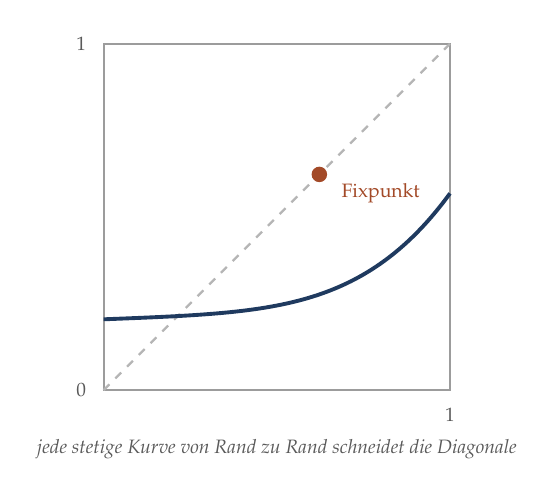
\begin{tikzpicture}[scale=1.0]
\draw[grau!60, line width=0.7pt] (0,0) rectangle (4.4,4.4);
\draw[grau!45, line width=0.8pt, dashed] (0,0) -- (4.4,4.4);
\draw[tief, line width=1.4pt] plot[smooth, samples=50, domain=0:4.4]
  ({\x}, {0.9 + 3.0*(\x/4.4)^3 - 1.4*(\x/4.4) + 0.5*sin(180*\x/4.4)});
\fill[akzent] (2.74,2.74) circle (2.8pt);
\node[font=\scriptsize, color=akzent, anchor=west] at (2.9,2.5) {Fixpunkt};
\node[font=\scriptsize, color=grau, anchor=east] at (-0.1,0) {$0$};
\node[font=\scriptsize, color=grau, anchor=east] at (-0.1,4.4) {$1$};
\node[font=\scriptsize, color=grau, anchor=north] at (4.4,-0.1) {$1$};
\node[font=\scriptsize\itshape, color=grau] at (2.2,-0.75) {jede stetige Kurve von Rand zu Rand schneidet die Diagonale};
\end{tikzpicture}
\end{center}

\schritt{Der allgemeine Fall}
\begin{center}
\begin{minipage}{0.88\textwidth}
\kursiv{In höheren Dimensionen gibt es keinen Zwischenwertsatz, und der Beweis wird erheblich schwieriger --- er benutzt Hilfsmittel der algebraischen Topologie oder, in einer elementareren Fassung, das Lemma von Sperner über gefärbte Triangulierungen. \textbf{Wir benutzen Satz 6.1 ohne Beweis}; das ist die erste der neun Auslassungen, die der Anhang tabelliert. Die Fundstelle ist Osborne und Rubinstein\zit{19}.}
\end{minipage}
\end{center}

\schritt{Warum alle drei Voraussetzungen nötig sind}
\begin{center}
{\small
\renewcommand{\arraystretch}{1.5}
\begin{tabular}{@{}P{2.2cm}P{3.0cm}P{3.2cm}@{}}
\toprule
\textbf{fehlt} & \textbf{Gegenbeispiel} & \textbf{Wirkung}\\
\midrule
kompakt & $f(x)=x+1$ auf $\R$ & läuft davon\\
konvex & Drehung eines Kreisrings & kein Fixpunkt\\
stetig & Sprungfunktion & springt über\\
\bottomrule
\end{tabular}}
\end{center}

\begin{center}
\begin{minipage}{0.88\textwidth}
\kursiv{Die mittlere Zeile ist die lehrreichste: Ein Kreisring ist kompakt, und eine Drehung um einen beliebigen Winkel ist stetig und bildet ihn auf sich ab --- aber sie hat keinen Fixpunkt. \textbf{Das Loch in der Mitte genügt}, und genau darauf zielen die topologischen Beweise des Satzes.}
\end{minipage}
\end{center}
\end{merksatz}

\section{Der Existenzsatz}

\begin{merksatz}
\boxtitel{Satz 6.2 --- Nash, 1950}
Jedes endliche Spiel --- beliebig viele Spieler, beliebig viele Strategien --- besitzt mindestens ein Nash-Gleichgewicht in gemischten Strategien.

\schritt{Schritt 1 --- Der Strategieraum}
Für Spieler $i$ mit $m_i$ reinen Strategien ist die Menge seiner Mischungen
\[ \Delta_i = \left\{ \vek\sigma_i \ : \ \sigma_{i,k} \ge 0, \ \textstyle\sum_k \sigma_{i,k} = 1 \right\} . \]

\begin{center}
{\small
\renewcommand{\arraystretch}{1.5}
\begin{tabular}{@{}P{2.4cm}P{6.2cm}@{}}
\toprule
\textbf{Nichtleer} & Jede reine Strategie liegt darin.\\
\textbf{Konvex} & Mischungen von Mischungen sind Mischungen.\\
\textbf{Kompakt} & Beschränkt durch $[0,1]^{m_i}$, abgeschlossen durch die Gleichung.\\
\bottomrule
\end{tabular}}
\end{center}

Das Produkt $\Delta = \Delta_1\times\cdots\times\Delta_n$ hat dieselben Eigenschaften.

\schritt{Schritt 2 --- Die Abbildung}
Für ein Profil $\vek\sigma$ und jede reine Strategie $k$ von Spieler $i$ setze
\[ g_{i,k}(\vek\sigma) = \max\bigl\{0,\ \Aus_i(k,\vek\sigma_{-i}) - \Aus_i(\vek\sigma)\bigr\} . \]

\begin{center}
\begin{minipage}{0.9\textwidth}
\textbf{$g_{i,k}$ misst, um wie viel Strategie $k$ besser wäre als das, was der Spieler gerade erhält} --- und ist null, wenn sie nicht besser ist.
\end{minipage}
\end{center}

Nun definiere $T: \Delta \to \Delta$ durch
\[ T(\vek\sigma)_{i,k} = \frac{\sigma_{i,k} + g_{i,k}(\vek\sigma)}{1 + \sum_{j} g_{i,j}(\vek\sigma)} . \]

\schritt{Schritt 3 --- $T$ ist wohldefiniert und stetig}
\kursiv{Wohldefiniert:} Zähler und Nenner sind nichtnegativ, der Nenner ist mindestens $1$. Die Summe über $k$ ergibt
\[ \frac{\sum_k \sigma_{i,k} + \sum_k g_{i,k}}{1+\sum_j g_{i,j}} = \frac{1 + \sum_k g_{i,k}}{1+\sum_j g_{i,j}} = 1 \quad \checkmark \]

\kursiv{Stetig:} $\Aus_i$ ist ein Polynom in den $\sigma$, also stetig; $\max\{0,\cdot\}$ ist stetig; Quotient mit Nenner $\ge 1$ ist stetig.

\schritt{Schritt 4 --- Brouwer anwenden}
Nach Satz 6.1 gibt es ein $\vek\sigma^{*}$ mit $T(\vek\sigma^{*}) = \vek\sigma^{*}$.

\schritt{Schritt 5 --- Fixpunkt heißt Gleichgewicht}
Schreibe $G_i := \sum_j g_{i,j}(\vek\sigma^{*})$. Die Fixpunktgleichung lautet
\[ \sigma_{i,k}^{*}\,(1+G_i) = \sigma_{i,k}^{*} + g_{i,k} \quad\Longrightarrow\quad \sigma_{i,k}^{*}\,G_i = g_{i,k} . \]

\kursiv{Annahme:} $G_i > 0$ für ein $i$.

Dann folgt für jedes $k$ mit $\sigma_{i,k}^{*} > 0$, dass $g_{i,k} > 0$ --- also ist \kursiv{jede benutzte} Strategie echt besser als der Durchschnitt $\Aus_i(\vek\sigma^{*})$.

\kursiv{Das ist unmöglich:} Der Durchschnitt ist
\[ \Aus_i(\vek\sigma^{*}) = \sum_k \sigma_{i,k}^{*}\,\Aus_i(k,\vek\sigma_{-i}^{*}) \]
--- ein gewichteter Mittelwert der Erträge der benutzten Strategien. Ein Mittelwert kann nicht kleiner sein als sein kleinster Summand.

\begin{center}
\begin{minipage}{0.9\textwidth}
\textbf{Also ist $G_i = 0$ für alle $i$, mithin $g_{i,k} = 0$ für alle $i,k$ --- keine Strategie ist besser als das Erreichte.} Das ist die Definition des Nash-Gleichgewichts. $\blacksquare$
\end{minipage}
\end{center}

\begin{center}
\begin{minipage}{0.88\textwidth}
\kursiv{Der Beweis ist eine halbe Seite lang und benutzt außer Brouwer nur die Beobachtung aus Satz 3.3: \textbf{Nicht jede benutzte Strategie kann überdurchschnittlich sein.} Von Neumanns Urteil \enquote{das ist trivial, ein Fixpunktsatz} beschreibt die Technik zutreffend --- und verfehlt, dass die Definition die Leistung war.}
\end{minipage}
\end{center}
\end{merksatz}

\begin{merksatz}
\boxtitel{Die Abbildung in Zahlen}
Am Feigheitsspiel aus Kapitel~5, symmetrisch gestartet bei $\vek\sigma = (\tfrac12,\tfrac12)$:

\begin{center}
{\small
\renewcommand{\arraystretch}{1.5}
\begin{tabular}{@{}P{1.4cm}P{2.0cm}P{2.0cm}P{2.4cm}@{}}
\toprule
\textbf{Schritt} & $\sigma_{\text{verzicht}}$ & \textbf{Ertrag} & \textbf{Gewinn bei Ausbau}\\
\midrule
$0$ & $0{,}5000$ & $2{,}750$ & $0{,}250$\\
$1$ & $0{,}4000$ & $2{,}520$ & $0{,}080$\\
$2$ & $0{,}3704$ & $2{,}440$ & $0{,}041$\\
$3$ & $0{,}3557$ & $2{,}399$ & $0{,}024$\\
$4$ & $0{,}3474$ & & \\
\midrule
$\infty$ & $\mathbf{0{,}3333}$ & $\mathbf{2{,}333}$ & $\mathbf{0}$\\
\bottomrule
\end{tabular}}
\end{center}

\kursiv{Zum ersten Schritt:} Ertrag $= \tfrac14(3+2+5+1) = 2{,}75$. Ausbau bringt $\tfrac12\cdot5+\tfrac12\cdot1 = 3$, also $g = 0{,}25$. Verzicht bringt $2{,}5 < 2{,}75$, also $g = 0$.
\[ T(\vek\sigma)_{\text{verzicht}} = \frac{0{,}5+0}{1+0{,}25} = 0{,}4 \quad \checkmark \]

\begin{center}
\begin{minipage}{0.9\textwidth}
\textbf{Die Folge nähert sich dem Gleichgewicht $\tfrac13$.} Der Gewinn schrumpft gegen null --- genau das kennzeichnet den Fixpunkt.
\end{minipage}
\end{center}

\begin{center}
\begin{minipage}{0.88\textwidth}
\kursiv{\textbf{Man darf daraus kein Verfahren machen.} Brouwer garantiert die Existenz eines Fixpunkts, nicht dass die Iteration zu ihm führt --- Fixpunkte können abstoßend sein. Hier klappt es; in anderen Spielen kreist die Folge dauerhaft, wie Kapitel~10 an einem Beispiel zeigen wird.}
\end{minipage}
\end{center}
\end{merksatz}

\section{Berechnung}

\begin{merksatz}
\boxtitel{Die Trägersuche}
Für zwei Spieler lässt sich das Verfahren aus Kapitel~3 übertragen.

\begin{center}
{\small
\renewcommand{\arraystretch}{1.5}
\begin{tabular}{@{}P{1.0cm}P{7.4cm}@{}}
\toprule
$1$ & Vermute je eine Teilmenge benutzter Strategien.\\
$2$ & Setze die Erträge innerhalb jedes Trägers gleich und löse.\\
$3$ & Prüfe Nichtnegativität und dass unbenutzte Strategien nicht besser sind.\\
\bottomrule
\end{tabular}}
\end{center}

\schritt{Der Aufwand}
\begin{center}
{\small
\renewcommand{\arraystretch}{1.48}
\begin{tabular}{@{}P{2.2cm}P{3.0cm}P{2.6cm}@{}}
\toprule
\textbf{Größe} & \textbf{Trägerpaare} & \\
\midrule
$2\times2$ & $9$ & von Hand\\
$3\times3$ & $49$ & mühsam\\
$5\times5$ & $961$ & Rechner\\
$10\times10$ & $1\,046\,529$ & \\
$20\times20$ & $\approx1{,}1\cdot10^{12}$ & \textcolor{akzent}{aussichtslos}\\
\bottomrule
\end{tabular}}
\end{center}

\begin{center}
\begin{minipage}{0.9\textwidth}
\textbf{Die Zahl der Trägerpaare beträgt $(2^{m}-1)(2^{n}-1)$ und wächst exponentiell.}
\end{minipage}
\end{center}
\end{merksatz}

\begin{merksatz}
\boxtitel{Der Unterschied zu Teil I}
\begin{center}
{\small
\renewcommand{\arraystretch}{1.52}
\begin{tabular}{@{}P{2.8cm}P{5.8cm}@{}}
\toprule
\textbf{Nullsumme} & Lineares Programm. Polynomiale Zeit, gesichert seit 1979.\\
\textbf{Nichtnull\-summe} & Kein lineares Programm --- es gibt keine gemeinsame Zielfunktion.\\
\bottomrule
\end{tabular}}
\end{center}

\begin{center}
\begin{minipage}{0.9\textwidth}
\textbf{Die Gegnerschaft macht das Problem leichter, nicht schwerer.}
\end{minipage}
\end{center}

\schritt{Satz 6.3 --- die Komplexität}
Das Auffinden eines Nash-Gleichgewichts ist vollständig für die Klasse $\mathsf{PPAD}$ --- und zwar bereits bei zwei Spielern.

\begin{center}
{\small
\renewcommand{\arraystretch}{1.5}
\begin{tabular}{@{}P{2.4cm}P{6.2cm}@{}}
\toprule
\textbf{Was $\mathsf{PPAD}$ ist} & Die Klasse der Suchprobleme, bei denen die Existenz einer Lösung aus einem Paritätsargument folgt --- Brouwer ist der Prototyp.\\
\textbf{Was das heißt} & Ein polynomiales Verfahren gilt als sehr unwahrscheinlich; bewiesen ist es nicht.\\
\bottomrule
\end{tabular}}
\end{center}

\begin{center}
\begin{minipage}{0.88\textwidth}
\kursiv{Die Lage entspricht der von $\mathsf{NP}$-Vollständigkeit in Band 19, Kapitel~12, mit einem Unterschied: \textbf{Hier ist die Existenz einer Lösung garantiert}, nur ihr Auffinden ist schwer. Solche Probleme passen nicht in $\mathsf{NP}$ im üblichen Sinn, weil es kein \enquote{Nein} gibt --- und deshalb brauchte es eine eigene Klasse, die \Person{Christos Papadimitriou} 1994 einführte.}
\end{minipage}
\end{center}

\schritt{Und was daraus folgt}
\begin{center}
\begin{minipage}{0.88\textwidth}
\kursiv{Wenn ein Gleichgewicht nicht in vertretbarer Zeit zu berechnen ist, stellt sich die Frage, ob Spieler es finden. \textbf{Ein Vorhersagebegriff, dessen Auswertung unerreichbar ist, verliert seinen Anspruch} --- so hat Papadimitriou das Ergebnis selbst gedeutet. Kapitel~15 kommt darauf zurück.}
\end{minipage}
\end{center}
\end{merksatz}

\section{Der Bruchfall}

\begin{warnung}
\boxtitelr{Was Satz 6.2 nicht liefert}
\begin{center}
{\small
\renewcommand{\arraystretch}{1.52}
\begin{tabular}{@{}P{2.4cm}P{6.2cm}@{}}
\toprule
\textbf{Kein Verfahren} & Der Beweis ist nicht konstruktiv. Brouwer sagt nicht, wo der Fixpunkt liegt.\\
\textbf{Keine Eindeutigkeit} & Es kann viele Gleichgewichte geben, mit ganz verschiedenen Auszahlungen.\\
\textbf{Keine Auswahl} & Welches erreicht wird, bleibt offen.\\
\textbf{Nur endlich} & Bei unendlichen Strategiemengen braucht man Zusatzannahmen.\\
\bottomrule
\end{tabular}}
\end{center}

\schritt{Zur ersten Zeile}
\begin{center}
\begin{minipage}{0.88\textwidth}
\kursiv{Es ist dasselbe Muster wie bei Shannons Kanalcodierungstheorem in Band 20, Kapitel~5: \textbf{Ein Existenzbeweis, der das Objekt nicht angibt.} Dort dauerte es sechzig Jahre bis zum konstruktiven Ersatz; hier spricht Satz 6.3 dafür, dass es ihn nicht geben wird.}
\end{minipage}
\end{center}

\schritt{Zur vierten Zeile}
Bei stetigen Strategieräumen gilt der Satz weiterhin, sofern die Auszahlungen stetig und die Räume konvex und kompakt sind.

\begin{center}
\begin{minipage}{0.88\textwidth}
\kursiv{Das ist der Satz von \Person{Glicksberg} von 1952. \textbf{Ohne Stetigkeit versagt er}: Ein Preiswettbewerb, in dem der Billigere den ganzen Markt bekommt, hat unstetige Auszahlungen --- und manche Varianten davon haben tatsächlich kein Gleichgewicht. Solche Fälle sind in der Wirtschaftstheorie keine Randerscheinung.}
\end{minipage}
\end{center}
\end{warnung}

\section{Übungsaufgaben}

\begin{aufgabe}
\boxtitel{Aufgabe 6.1 --- Brouwer nachprüfen}
\begin{center}
{\small
\renewcommand{\arraystretch}{1.4}
\begin{tabular}{@{}P{0.8cm}P{7.6cm}@{}}
\toprule
(a) & Bestimmen Sie den Fixpunkt von $f(x) = \tfrac14 x + \tfrac12$ auf $[0,1]$.\\
(b) & Zeigen Sie, dass $f(x) = x+1$ auf $\R$ keinen hat, und benennen Sie die verletzte Voraussetzung.\\
(c) & Hat $f(x) = 1-x$ auf $[0,1]$ einen Fixpunkt?\\
\bottomrule
\end{tabular}}
\end{center}

\loesung
\schritt{(a)}
\[ x = \tfrac14 x + \tfrac12 \quad\Longrightarrow\quad \tfrac34 x = \tfrac12 \quad\Longrightarrow\quad x = \tfrac23 \]

\kursiv{Probe:} $\tfrac14\cdot\tfrac23 + \tfrac12 = \tfrac16 + \tfrac36 = \tfrac46 = \tfrac23$ \checkmark

\kursiv{Voraussetzungen:} $[0,1]$ ist konvex und kompakt; $f$ ist stetig; $f([0,1]) = [\tfrac12,\tfrac34] \subset [0,1]$ \checkmark

\schritt{(b)}
\[ x = x+1 \quad\Longrightarrow\quad 0 = 1 \]
Unlösbar.

\begin{center}
\begin{minipage}{0.9\textwidth}
\textbf{Verletzt ist die Kompaktheit:} $\R$ ist nicht beschränkt.
\end{minipage}
\end{center}

\kursiv{Konvexität und Stetigkeit sind erfüllt.} Es genügt also eine verletzte Voraussetzung.

\schritt{(c)}
\[ x = 1-x \quad\Longrightarrow\quad x = \tfrac12 \]

Ja --- und zwar genau einer.

\begin{center}
\begin{minipage}{0.88\textwidth}
\kursiv{Bemerkenswert: Diese Abbildung ist eine Spiegelung, also eine Bewegung ohne Zusammenziehung. \textbf{Brouwer verlangt keine Kontraktion} --- anders als der Fixpunktsatz von Banach, der zusätzlich die Eindeutigkeit und ein Verfahren liefert. Der Preis der schwächeren Voraussetzung ist genau das, was der Bruchfall benennt: kein Verfahren, keine Eindeutigkeit.}
\end{minipage}
\end{center}

\schritt{Schritt 4 --- Die Iteration bei (c)}
\[ 0{,}3 \ \to\ 0{,}7 \ \to\ 0{,}3 \ \to\ 0{,}7 \ \to\ \cdots \]

\begin{center}
\begin{minipage}{0.9\textwidth}
\textbf{Die Folge kreist und erreicht den Fixpunkt nie} --- obwohl er existiert und eindeutig ist.
\end{minipage}
\end{center}

\kursiv{Bei (a) dagegen:} $0{,}3 \to 0{,}575 \to 0{,}644 \to 0{,}661 \to 0{,}665 \to \cdots \to \tfrac23$, denn $|f'| = \tfrac14 < 1$.

\begin{center}
\begin{minipage}{0.86\textwidth}
\kursiv{Das ist der Grund für die Warnung am Ende von Abschnitt 6.3 --- in Zahlen. \textbf{Existenz und Erreichbarkeit sind zwei verschiedene Dinge}, und die Abbildung $T$ aus Satz 6.2 ist im Allgemeinen keine Kontraktion.}
\end{minipage}
\end{center}
\end{aufgabe}

\begin{aufgabe}
\boxtitel{Aufgabe 6.2 --- Die Nash-Abbildung rechnen}
Führen Sie im Gefangenendilemma aus Kapitel~5 einen Schritt der Abbildung $T$ aus, ausgehend von $\vek\sigma = (\tfrac12,\tfrac12)$ für beide.

\loesung
\schritt{Schritt 1 --- Die Matrix}
\begin{center}
{\small
\renewcommand{\arraystretch}{1.55}
\begin{tabular}{@{}P{2.4cm}P{2.0cm}P{2.0cm}@{}}
\toprule
& \textbf{zurück} & \textbf{frei}\\
\midrule
\textbf{zurück} & $(3,3)$ & $(0,5)$\\
\textbf{frei} & $(5,0)$ & $(1,1)$\\
\bottomrule
\end{tabular}}
\end{center}

\schritt{Schritt 2 --- Der gegenwärtige Ertrag}
\[ \Aus_1(\vek\sigma) = \tfrac14(3+0+5+1) = \tfrac94 = 2{,}25 \]

\schritt{Schritt 3 --- Die Erträge der reinen Strategien}
\begin{center}
\renewcommand{\arraystretch}{1.48}
\begin{tabular}{@{}P{2.8cm}P{2.6cm}P{2.0cm}@{}}
\toprule
\textbf{Strategie} & \textbf{Rechnung} & \textbf{Ertrag}\\
\midrule
zurückhalten & $\tfrac12\cdot3+\tfrac12\cdot0$ & $1{,}5$\\
frei einsetzen & $\tfrac12\cdot5+\tfrac12\cdot1$ & $3{,}0$\\
\bottomrule
\end{tabular}
\end{center}

\schritt{Schritt 4 --- Die Gewinne}
\[ g_{\text{zurück}} = \max\{0,\ 1{,}5-2{,}25\} = 0 \]
\[ g_{\text{frei}} = \max\{0,\ 3{,}0-2{,}25\} = 0{,}75 \]

\schritt{Schritt 5 --- Der Schritt}
\[ T(\vek\sigma)_{\text{zurück}} = \frac{0{,}5 + 0}{1+0{,}75} = \frac{0{,}5}{1{,}75} = \tfrac27 \approx 0{,}286 \]
\[ T(\vek\sigma)_{\text{frei}} = \frac{0{,}5+0{,}75}{1{,}75} = \frac{1{,}25}{1{,}75} = \tfrac57 \approx 0{,}714 \]

\kursiv{Probe:} $\tfrac27 + \tfrac57 = 1$ \checkmark

\schritt{Schritt 6 --- Die Richtung}
\begin{center}
\begin{minipage}{0.9\textwidth}
\textbf{Der Anteil des Zurückhaltens sinkt von $0{,}5$ auf $0{,}286$} --- die Abbildung strebt zum Gleichgewicht $(0,1)$.
\end{minipage}
\end{center}

\schritt{Schritt 7 --- Der Fixpunkt geprüft}
Bei $\vek\sigma = (0,1)$, also beidseitig freier Einsatz:
\begin{center}
\renewcommand{\arraystretch}{1.48}
\begin{tabular}{@{}P{2.8cm}P{1.8cm}P{2.4cm}@{}}
\toprule
\textbf{Strategie} & \textbf{Ertrag} & \textbf{Gewinn}\\
\midrule
zurückhalten & $0$ & $\max\{0,-1\} = 0$\\
frei einsetzen & $1$ & $\max\{0,0\} = 0$\\
\bottomrule
\end{tabular}
\end{center}

Gegenwärtiger Ertrag: $1$. Alle Gewinne null, also $G = 0$:
\[ T(\vek\sigma)_{\text{frei}} = \frac{1+0}{1+0} = 1 \quad \checkmark \]

\begin{center}
\begin{minipage}{0.88\textwidth}
\kursiv{Die Abbildung lässt das Gleichgewicht unverändert --- so muss es sein. \textbf{Man beachte, dass das Zurückhalten hier einen \kursiv{negativen} Vorteil hat} und die Abschneidung bei null greift. Ohne sie wäre $T$ nicht wohldefiniert, weil der Nenner null oder negativ werden könnte.}
\end{minipage}
\end{center}
\end{aufgabe}

\begin{aufgabe}
\boxtitel{Aufgabe 6.3 --- Trägersuche}
Bestimmen Sie alle Gleichgewichte:
\begin{center}
{\small
\renewcommand{\arraystretch}{1.6}
\begin{tabular}{@{}P{1.6cm}P{2.0cm}P{2.0cm}@{}}
\toprule
& \textbf{L} & \textbf{R}\\
\midrule
\textbf{O} & $(2,\ 1)$ & $(0,\ 0)$\\
\textbf{M} & $(0,\ 0)$ & $(1,\ 2)$\\
\textbf{U} & $(1,\ 1)$ & $(1,\ 1)$\\
\bottomrule
\end{tabular}}
\end{center}

\loesung
\schritt{Schritt 1 --- Reine Gleichgewichte}
\begin{center}
{\small
\renewcommand{\arraystretch}{1.48}
\begin{tabular}{@{}P{1.6cm}P{2.4cm}P{2.4cm}P{1.2cm}@{}}
\toprule
\textbf{Feld} & \textbf{Zeile wechselt} & \textbf{Spalte wechselt} & \\
\midrule
$(\text{O},\text{L})$ & $2\to0$ bzw. $1$ & $1\to0$ & \textcolor{gruen}{GG}\\
$(\text{M},\text{R})$ & $1\to0$ bzw. $1$ & $2\to0$ & \textcolor{gruen}{GG}\\
$(\text{U},\text{L})$ & $1\to2$ & --- & ---\\
$(\text{U},\text{R})$ & $1\to1$ bzw. $0$ & $1\to0$ & \textcolor{gruen}{GG}\\
\bottomrule
\end{tabular}}
\end{center}

\kursiv{Zu $(\text{U},\text{R})$:} Der Zeilenspieler erhält $1$; O brächte $0$, M brächte $1$. Er kann sich also nicht verbessern. Der Spaltenspieler erhält $1$; L brächte ebenfalls $1$.

\begin{center}
\begin{minipage}{0.88\textwidth}
\kursiv{Hier liegt ein \kursiv{schwaches} Gleichgewicht vor: Abweichen kostet nichts, bringt aber auch nichts. \textbf{Das zählt nach Definition 4.3 als Gleichgewicht}, weil die Definition nur \enquote{nicht besser} verlangt --- ein Punkt, auf den Kapitel~7 zurückkommt.}
\end{minipage}
\end{center}

\kursiv{Und $(\text{U},\text{L})$:} Der Zeilenspieler würde zu O wechseln ($2>1$). Kein Gleichgewicht.

\schritt{Schritt 2 --- Gemischte mit Träger $\{\text{O},\text{M}\}$}
Der Spaltenspieler sei gleichgültig zwischen L und R:
\[ p\cdot1 + (1-p)\cdot0 = p\cdot0 + (1-p)\cdot2 \]
\[ p = 2-2p \quad\Longrightarrow\quad p = \tfrac23 \]

Der Zeilenspieler sei gleichgültig zwischen O und M:
\[ q\cdot2 + (1-q)\cdot0 = q\cdot0 + (1-q)\cdot1 \]
\[ 2q = 1-q \quad\Longrightarrow\quad q = \tfrac13 \]

\schritt{Schritt 3 --- Die Probe für die unbenutzte Zeile}
Ertrag des Zeilenspielers: $2\cdot\tfrac13 = \tfrac23$.

Zeile U brächte gegen $\vek q$:
\[ \tfrac13\cdot1 + \tfrac23\cdot1 = 1 \ >\ \tfrac23 \]

\begin{center}
\begin{minipage}{0.9\textwidth}
\textcolor{akzent}{\textbf{Die Vermutung scheitert.}} Der Zeilenspieler würde auf U ausweichen.
\end{minipage}
\end{center}

\schritt{Schritt 4 --- Träger $\{\text{O},\text{U}\}$ versuchen}
Der Zeilenspieler sei gleichgültig zwischen O und U:
\[ 2q + 0(1-q) = 1q + 1(1-q) = 1 \quad\Longrightarrow\quad q = \tfrac12 \]

Der Spaltenspieler benutzt beide Spalten, muss also gleichgültig sein. Mit $p$ auf O und $1-p$ auf U:
\[ p\cdot1 + (1-p)\cdot1 = p\cdot0 + (1-p)\cdot1 \]
\[ 1 = 1-p \quad\Longrightarrow\quad p = 0 \]

\begin{center}
\begin{minipage}{0.9\textwidth}
\textbf{Also $p=0$ --- die Zeile O wird gar nicht benutzt.} Es bleibt $(\text{U},\ \vek q)$ mit beliebigem $q$.
\end{minipage}
\end{center}

\schritt{Schritt 5 --- Diese Familie prüfen}
Spielt der Zeilenspieler U und der Spaltenspieler eine beliebige Mischung $\vek q$:

\begin{center}
\renewcommand{\arraystretch}{1.48}
\begin{tabular}{@{}P{1.8cm}P{2.8cm}P{2.4cm}@{}}
\toprule
\textbf{Zeile} & \textbf{Ertrag gegen $\vek q$} & \\
\midrule
O & $2q$ & \\
M & $1-q$ & \\
U & $1$ & \\
\bottomrule
\end{tabular}
\end{center}

U ist beste Antwort genau dann, wenn $2q \le 1$ und $1-q \le 1$, also
\[ q \ \le\ \tfrac12 . \]

Der Spaltenspieler erhält gegen U in beiden Spalten $1$ --- er ist stets gleichgültig. \checkmark

\begin{center}
\begin{minipage}{0.9\textwidth}
\textbf{Es gibt ein ganzes Kontinuum von Gleichgewichten:} $(\text{U},\ (q,1-q))$ für alle $q \le \tfrac12$.
\end{minipage}
\end{center}

\schritt{Schritt 6 --- Die Bilanz}
\begin{center}
{\small
\renewcommand{\arraystretch}{1.5}
\begin{tabular}{@{}P{3.2cm}P{2.0cm}P{2.2cm}@{}}
\toprule
\textbf{Gleichgewicht} & \textbf{Aus\-zahlung} & \\
\midrule
$(\text{O},\text{L})$ & $(2,1)$ & rein\\
$(\text{M},\text{R})$ & $(1,2)$ & rein\\
$(\text{U},\ q\le\tfrac12)$ & $(1,1)$ & \textcolor{akzent}{Kontinuum}\\
\bottomrule
\end{tabular}}
\end{center}

\begin{center}
\begin{minipage}{0.88\textwidth}
\kursiv{Die Zahl der Gleichgewichte ist hier nicht ungerade, sondern unendlich --- der Satz von Wilson aus Aufgabe 4.1 gilt nur für \kursiv{generische} Auszahlungen, und die Gleichheit der Einträge in Zeile U ist genau die Ausnahme. \textbf{Solche Entartungen sind in konstruierten Beispielen die Regel und in gemessenen Daten die Ausnahme}, was die praktische Bedeutung des Satzes einschränkt: Reale Auszahlungen sind geschätzt, und Schätzungen sind nie exakt gleich.}
\end{minipage}
\end{center}
\end{aufgabe}

\begin{geschichte}
\boxtitelg{Ein Beweis in zwei Fassungen}
Nashs Dissertation von 1950 enthält den Existenzbeweis über den Fixpunktsatz von \Person{Kakutani} --- eine Verallgemeinerung von Brouwer auf mengenwertige Abbildungen.

\begin{center}
\begin{minipage}{0.9\textwidth}
\kursiv{Man bildet jedes Profil auf die Menge der besten Antworten ab. Ein Fixpunkt dieser Abbildung ist unmittelbar ein Gleichgewicht --- der Beweis ist kürzer als der in Abschnitt 6.3, benutzt aber das schwerere Hilfsmittel.}
\end{minipage}
\end{center}

\schritt{Die zweite Fassung}
1951 veröffentlichte Nash in den \kursiv{Annals of Mathematics} einen Beweis, der mit Brouwer auskommt --- genau die Abbildung $T$ aus Satz 6.2.

\begin{center}
\begin{minipage}{0.9\textwidth}
\kursiv{\textbf{Der Aufsatz umfasst knapp neun Seiten.} Er enthält neben dem Beweis den Begriff des symmetrischen Gleichgewichts und ein Beispiel mit drei Spielern. Dass Nash denselben Satz zweimal bewies, hatte einen Grund: Der zweite Beweis benutzt weniger und ist damit grundsätzlicher.}
\end{minipage}
\end{center}

\schritt{Kakutani und von Neumann}
\Person{Shizuo Kakutani} hatte seinen Satz 1941 bewiesen --- ausdrücklich, um von Neumanns Minimax-Beweis zu vereinfachen.

\begin{center}
\begin{minipage}{0.9\textwidth}
\kursiv{Von Neumanns Originalbeweis von 1928 war lang und technisch; Kakutanis Fassung passt auf eine Seite. \textbf{Nash benutzte also ein Werkzeug, das eigens für von Neumanns Satz geschaffen worden war} --- was dessen Bemerkung, die Sache sei trivial, in ein etwas anderes Licht rückt.}
\end{minipage}
\end{center}

\schritt{Brouwer selbst}
\Person{Luitzen Brouwer} (1881--1966) bewies seinen Satz 1911 und verwarf ihn später.

\begin{center}
\begin{minipage}{0.9\textwidth}
\kursiv{Er wurde zum Begründer des Intuitionismus, der nicht konstruktive Existenzbeweise ablehnt --- und sein eigener Fixpunktsatz ist das Musterbeispiel eines solchen Beweises. \textbf{Brouwer erklärte ihn für ungültig nach seinen späteren Maßstäben.} Dass die halbe Wirtschaftstheorie auf einem Satz ruht, den sein Urheber nicht mehr anerkannte, gehört zu den bemerkenswerteren Fußnoten dieses Fachs.}
\end{minipage}
\end{center}
\end{geschichte}

\begin{forschung}
\boxtitelp{Gleichgewichte berechnen}
\begin{center}
{\small
\renewcommand{\arraystretch}{1.45}
\begin{tabular}{@{}P{2.8cm}P{5.4cm}@{}}
\toprule
\textbf{Lemke-Howson} & Ein Wegverfolgungsverfahren für zwei Spieler; findet stets eines, braucht im schlechtesten Fall exponentiell lange.\\
\textbf{Näherungen} & Gleichgewichte, bei denen sich niemand um mehr als $\varepsilon$ verbessern kann.\\
\textbf{Korreliert} & Ein weiterer Gleichgewichtsbegriff --- in polynomialer Zeit berechenbar.\\
\bottomrule
\end{tabular}}
\end{center}

\schritt{Zur ersten Zeile}
Das Verfahren stammt von 1964 und ist dem Simplexverfahren verwandt.

\begin{center}
\begin{minipage}{0.88\textwidth}
\kursiv{Dass es im schlechtesten Fall exponentiell lange braucht, wurde erst 2004 gezeigt --- mit Beispielen, die den Klee-Minty-Würfeln aus Band 19, Kapitel~3 entsprechen. \textbf{Dasselbe Muster wie dort: ein Verfahren, das in der Praxis gut läuft und im Beweis versagt.}}
\end{minipage}
\end{center}

\schritt{Zur dritten Zeile}
Das \Begriff{korrelierte Gleichgewicht} von \Person{Robert Aumann} (1974) erlaubt einen gemeinsamen Zufallsmechanismus, dessen Empfehlungen jeder befolgen möchte.

\begin{center}
\begin{minipage}{0.88\textwidth}
\kursiv{Eine Ampel ist das Musterbeispiel: Sie empfiehlt dem einen Halten, dem anderen Fahren, und beide folgen gern. \textbf{Solche Gleichgewichte sind durch ein lineares Programm zu finden} --- also leicht --- und können Auszahlungen erreichen, die kein Nash-Gleichgewicht erreicht. Im Feigheitsspiel aus Kapitel~5 etwa lassen sich die schlechten $(1,1)$ vollständig vermeiden, was das gemischte Gleichgewicht nicht kann.}
\end{minipage}
\end{center}
\end{forschung}

\begin{merksatz}
\boxtitel{Was Sie jetzt können}
\begin{center}
\renewcommand{\arraystretch}{1.5}
\begin{tabular}{@{}P{3.0cm}P{5.6cm}@{}}
\toprule
\textbf{Satz 6.1} & Brouwer: stetig, konvex, kompakt\\
\textbf{Satz 6.2} & jedes endliche Spiel hat eines\\
\textbf{Die Abbildung} & Gewinn dazurechnen, normieren\\
\textbf{Satz 6.3} & $\mathsf{PPAD}$-vollständig\\
\textbf{Der Vorbehalt} & Existenz ist nicht Erreichbarkeit\\
\bottomrule
\end{tabular}
\end{center}

\begin{center}
\begin{minipage}{0.88\textwidth}
\kursiv{Damit endet Teil~II. Bisher wurde einmal gezogen, gleichzeitig und ohne Vorgeschichte. Ab Kapitel~7 gibt es eine Reihenfolge --- und aus der Drohung wird die Frage, ob man sie glauben muss.}
\end{minipage}
\end{center}
\end{merksatz}

\part{Über die Zeit}

\chapter{Reihenfolge und Glaubwürdigkeit}

\section{Dasselbe Spiel, nacheinander gespielt}

\begin{merksatz}
\boxtitel{Der Leitfall, umgestellt}
Das Ausbauspiel aus Kapitel~5 hatte drei Gleichgewichte und keine Antwort darauf, welches eintritt. Nun ziehe das Klinikum zuerst, und das Marienhospital sehe die Entscheidung.

\begin{center}
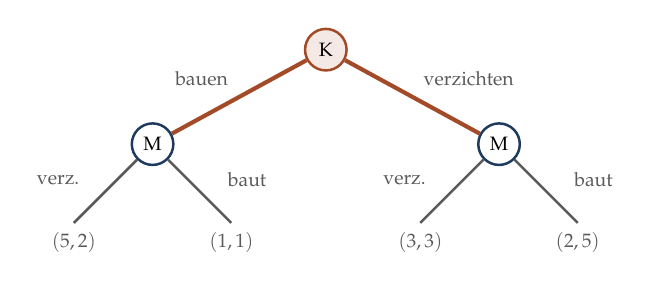
\begin{tikzpicture}[scale=1.0]
\node[knotenr] (w) at (0,2.4) {K};
\node[knotenb] (a) at (-2.2,1.2) {M};
\node[knotenb] (b) at (2.2,1.2) {M};
\draw[kanted] (w)--(a) node[midway,above left,font=\scriptsize,color=grau] {bauen};
\draw[kanted] (w)--(b) node[midway,above right,font=\scriptsize,color=grau] {verzichten};
\foreach \x/\p/\lab in {-3.2/a/verzicht., -1.2/a/bauen, 1.2/b/verzicht., 3.2/b/bauen}
  \draw[kante] (\p)--(\x,0.2);
\node[font=\scriptsize, color=grau, anchor=north] at (-3.2,0.2) {$(5,2)$};
\node[font=\scriptsize, color=grau, anchor=north] at (-1.2,0.2) {$(1,1)$};
\node[font=\scriptsize, color=grau, anchor=north] at (1.2,0.2) {$(3,3)$};
\node[font=\scriptsize, color=grau, anchor=north] at (3.2,0.2) {$(2,5)$};
\node[font=\scriptsize, color=grau] at (-3.4,0.75) {verz.};
\node[font=\scriptsize, color=grau] at (-1.0,0.75) {baut};
\node[font=\scriptsize, color=grau] at (1.0,0.75) {verz.};
\node[font=\scriptsize, color=grau] at (3.4,0.75) {baut};
\end{tikzpicture}
\end{center}

\begin{center}
\begin{minipage}{0.9\textwidth}
\textbf{Die Auszahlungen sind unverändert.} Nur die Reihenfolge ist neu --- und das genügt, um die Unbestimmtheit aufzulösen.
\end{minipage}
\end{center}
\end{merksatz}

\begin{definition}
\boxtitelm{Definition 7.1 --- Spiel in extensiver Form}
Ein \Begriff{Spielbaum} besteht aus Knoten und Kanten. An jedem inneren Knoten zieht ein Spieler; jeder Endknoten trägt einen Auszahlungsvektor.

Eine \Begriff{Strategie} eines Spielers ist ein \kursiv{vollständiger Plan}: für jeden Knoten, an dem er ziehen könnte, eine Festlegung.
\end{definition}

\begin{merksatz}
\boxtitel{Der Strategiebegriff ist überraschend umfangreich}
Das Marienhospital zieht nur einmal --- aber es kann an zwei verschiedenen Knoten am Zug sein.

\begin{center}
{\small
\renewcommand{\arraystretch}{1.5}
\begin{tabular}{@{}P{2.2cm}P{2.6cm}P{2.8cm}@{}}
\toprule
\textbf{Strategie} & \textbf{nach K baut} & \textbf{nach K verzichtet}\\
\midrule
$VV$ & verzichten & verzichten\\
$VB$ & verzichten & bauen\\
$BV$ & bauen & verzichten\\
$BB$ & bauen & bauen\\
\bottomrule
\end{tabular}}
\end{center}

\begin{center}
\begin{minipage}{0.9\textwidth}
\textbf{Vier Strategien für einen einzigen Zug.} Eine Strategie legt auch fest, was man in Lagen täte, die gar nicht eintreten.
\end{minipage}
\end{center}

\begin{center}
\begin{minipage}{0.88\textwidth}
\kursiv{Das wirkt umständlich und ist der Kern des Kapitels. \textbf{Genau diese Festlegungen für nicht eintretende Lagen sind die Drohungen} --- und die Frage, ob man sie glauben muss, ist die Frage nach ihrer Optimalität im jeweiligen Zweig. Bei größeren Bäumen wächst die Zahl der Strategien rasch: Bei $k$ Entscheidungsknoten mit je zwei Zügen sind es $2^{k}$.}
\end{minipage}
\end{center}
\end{merksatz}

\section{Rückwärtsinduktion}

\begin{merksatz}
\boxtitel{Das Verfahren}
Man löst den Baum von den Blättern her auf.

\begin{center}
{\small
\renewcommand{\arraystretch}{1.5}
\begin{tabular}{@{}P{1.0cm}P{7.4cm}@{}}
\toprule
$1$ & Betrachte einen Knoten, dessen Nachfolger alle Endknoten sind.\\
$2$ & Der dort ziehende Spieler wählt seine beste Auszahlung.\\
$3$ & Ersetze den Knoten durch diesen Auszahlungsvektor.\\
$4$ & Wiederhole, bis nur die Wurzel bleibt.\\
\bottomrule
\end{tabular}}
\end{center}

\schritt{Der Leitfall}
\kursiv{Knoten nach \enquote{K baut}:} Das Marienhospital vergleicht $2$ (verzichten) mit $1$ (bauen).
\[ \Longrightarrow \text{verzichten}, \quad \text{Wert } (5,2) \]

\kursiv{Knoten nach \enquote{K verzichtet}:} Es vergleicht $3$ mit $5$.
\[ \Longrightarrow \text{bauen}, \quad \text{Wert } (2,5) \]

\kursiv{Die Wurzel:} Das Klinikum vergleicht $5$ mit $2$.
\[ \Longrightarrow \text{bauen} \]

\begin{center}
\begin{minipage}{0.9\textwidth}
\textbf{Ergebnis $(5,2)$ --- das Klinikum setzt sich durch, weil es zuerst zieht.}
\end{minipage}
\end{center}

\begin{center}
\begin{minipage}{0.88\textwidth}
\kursiv{Das ist der \Begriff{Erstzieher-Vorteil}, und er ist die formale Fassung dessen, was Aufgabe 5.2 als Festlegung beschrieb. \textbf{Der Vorteil entsteht nicht durch den früheren Zug, sondern durch dessen Sichtbarkeit.} Zöge das Klinikum zuerst, ohne dass das Marienhospital es erführe, so läge wieder das Spiel aus Kapitel~5 vor.}
\end{minipage}
\end{center}
\end{merksatz}

\begin{merksatz}
\boxtitel{Satz 7.2 --- Zermelo, 1913}
Jedes endliche Spiel mit vollkommener Information --- alle Züge sind sichtbar, kein Zufall --- besitzt ein Gleichgewicht in reinen Strategien.

\schritt{Beweis}
Rückwärtsinduktion liefert eines. Da der Baum endlich ist, bricht das Verfahren ab; an jedem Knoten existiert ein Maximum, weil endlich viele Züge zur Wahl stehen. $\blacksquare$

\begin{center}
\begin{minipage}{0.9\textwidth}
\textbf{Man braucht hier keinen Fixpunktsatz und keine gemischten Strategien.}
\end{minipage}
\end{center}

\begin{center}
\begin{minipage}{0.88\textwidth}
\kursiv{Für Schach heißt das: Entweder kann Weiß gewinnen, oder Schwarz, oder beide können ein Remis erzwingen. \textbf{Welches der drei zutrifft, ist unbekannt} --- der Baum hat etwa $10^{120}$ Knoten. Dame ist seit 2007 gelöst (Remis bei beiderseits bestem Spiel); Schach nicht und voraussichtlich nie.}
\end{minipage}
\end{center}
\end{merksatz}

\section{Unglaubwürdige Drohungen}

\begin{merksatz}
\boxtitel{Die Normalform desselben Spiels}
\begin{center}
{\small
\renewcommand{\arraystretch}{1.6}
\begin{tabular}{@{}P{1.8cm}P{1.6cm}P{1.6cm}P{1.6cm}P{1.6cm}@{}}
\toprule
& $VV$ & $VB$ & $BV$ & $BB$\\
\midrule
\textbf{bauen} & $(5,2)$ & $(5,2)$ & $(1,1)$ & $(1,1)$\\
\textbf{verzicht.} & $(3,3)$ & $(2,5)$ & $(3,3)$ & $(2,5)$\\
\bottomrule
\end{tabular}}
\end{center}

\schritt{Die Nash-Gleichgewichte}
\begin{center}
{\small
\renewcommand{\arraystretch}{1.5}
\begin{tabular}{@{}P{2.6cm}P{2.0cm}P{3.0cm}@{}}
\toprule
\textbf{Gleichgewicht} & \textbf{Aus\-zahlung} & \\
\midrule
$(\text{bauen},\ VV)$ & $(5,2)$ & \\
$(\text{bauen},\ VB)$ & $(5,2)$ & \textcolor{gruen}{Rückwärts\-induktion}\\
$(\text{verzicht.},\ BB)$ & $(2,5)$ & \textcolor{akzent}{Drohung}\\
\bottomrule
\end{tabular}}
\end{center}

\begin{center}
\begin{minipage}{0.9\textwidth}
\textbf{Drei Gleichgewichte --- und eines davon widerspricht der Rückwärtsinduktion.}
\end{minipage}
\end{center}

\schritt{Das dritte genauer}
Die Strategie $BB$ besagt: \enquote{Ich baue, was immer du tust.}

\kursiv{Prüfung:} Gilt das Klinikum als abweichend --- es baut ---, so führt $BB$ zu $(1,1)$. Das Klinikum bliebe also lieber bei $2$. Die Drohung wirkt.

\kursiv{Der Einwand:} Baut das Klinikum tatsächlich, so steht das Marienhospital vor der Wahl $2$ gegen $1$.

\begin{center}
\begin{minipage}{0.9\textwidth}
\textbf{Es würde nicht bauen.} Die Drohung ist ein Gleichgewicht, weil sie nie auf die Probe gestellt wird --- und genau deshalb kostet sie nichts.
\end{minipage}
\end{center}

\begin{center}
\begin{minipage}{0.88\textwidth}
\kursiv{Das ist die Schwäche des Nash-Begriffs bei sequentiellen Spielen: \textbf{Er prüft nur, was auf dem tatsächlich beschrittenen Pfad geschieht.} Was jemand abseits des Pfades angekündigt hat, bleibt ungeprüft, weil es dort keine Abweichung gibt, die sich lohnen könnte.}
\end{minipage}
\end{center}
\end{merksatz}

\begin{definition}
\boxtitelm{Definition 7.3 --- Teilspielperfektheit}
Ein \Begriff{Teilspiel} ist der Baum unterhalb eines Knotens, sofern er für sich ein Spiel bildet.

Ein Strategieprofil heißt \Begriff{teilspielperfekt}, wenn es in \kursiv{jedem} Teilspiel ein Nash-Gleichgewicht ist --- auch in solchen, die nicht erreicht werden.
\end{definition}

\begin{merksatz}
\boxtitel{Die Prüfung im Leitfall}
\begin{center}
{\small
\renewcommand{\arraystretch}{1.5}
\begin{tabular}{@{}P{2.2cm}P{2.6cm}P{3.0cm}@{}}
\toprule
\textbf{Strategie} & \textbf{nach K baut} & \textbf{nach K verzichtet}\\
\midrule
$VV$ & $2$ \textcolor{gruen}{optimal} & $3 < 5$ \textcolor{akzent}{nicht optimal}\\
$VB$ & $2$ \textcolor{gruen}{optimal} & $5$ \textcolor{gruen}{optimal}\\
$BB$ & $1 < 2$ \textcolor{akzent}{nicht} & $5$ \textcolor{gruen}{optimal}\\
\bottomrule
\end{tabular}}
\end{center}

\begin{center}
\begin{minipage}{0.9\textwidth}
\textbf{Nur $(\text{bauen},\ VB)$ ist teilspielperfekt} --- genau die Lösung der Rückwärtsinduktion.
\end{minipage}
\end{center}

\begin{center}
\begin{minipage}{0.88\textwidth}
\kursiv{Bemerkenswert ist, dass auch $(\text{bauen}, VV)$ herausfällt, obwohl es dieselbe Auszahlung liefert. \textbf{Teilspielperfektheit prüft das Verhalten, nicht das Ergebnis} --- und $VV$ enthält die Absicht, nach einem Verzicht des Klinikums ebenfalls zu verzichten, was dort nicht optimal wäre.}
\end{minipage}
\end{center}

\schritt{Satz 7.4}
Bei vollkommener Information sind die teilspielperfekten Gleichgewichte genau die Lösungen der Rückwärtsinduktion.

\kursiv{Grund:} Jeder Entscheidungsknoten beginnt ein Teilspiel; die Forderung dort ist genau die Wahl des Maximums.
\end{merksatz}

\section{Wenn nicht alles sichtbar ist}

\begin{merksatz}
\boxtitel{Informationsmengen}
Zieht ein Spieler, ohne zu wissen, an welchem Knoten er steht, so fasst man diese Knoten zu einer \Begriff{Informationsmenge} zusammen.

\begin{center}
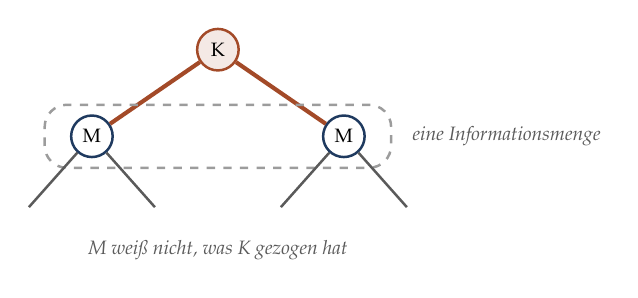
\begin{tikzpicture}[scale=1.0]
\node[knotenr] (w) at (0,2.2) {K};
\node[knotenb] (a) at (-1.6,1.1) {M};
\node[knotenb] (b) at (1.6,1.1) {M};
\draw[kanted] (w)--(a); \draw[kanted] (w)--(b);
\draw[grau!60, line width=0.9pt, dashed, rounded corners=8pt]
  (-2.2,0.7) rectangle (2.2,1.5);
\node[font=\scriptsize\itshape, color=grau, anchor=west] at (2.35,1.1) {eine Informationsmenge};
\foreach \x/\p in {-2.4/a, -0.8/a, 0.8/b, 2.4/b} \draw[kante] (\p)--(\x,0.2);
\node[font=\scriptsize\itshape, color=grau] at (0,-0.35) {M weiß nicht, was K gezogen hat};
\end{tikzpicture}
\end{center}

\begin{center}
\begin{minipage}{0.9\textwidth}
\textbf{Eine Strategie muss dann an allen Knoten derselben Menge dasselbe vorschreiben.}
\end{minipage}
\end{center}

\begin{center}
\begin{minipage}{0.88\textwidth}
\kursiv{Damit lassen sich gleichzeitige Züge als Baum darstellen --- Teil~I und II sind Sonderfälle von Teil~III. \textbf{Das Spiel aus Kapitel~5 ist derselbe Baum wie der vom Kapitelanfang}, nur mit den beiden M-Knoten in einer Informationsmenge. Der Erstzieher-Vorteil verschwindet dann vollständig.}
\end{minipage}
\end{center}

\schritt{Satz 7.5 --- Kuhn, 1953}
Bei \Begriff{perfektem Erinnerungsvermögen} --- kein Spieler vergisst, was er wusste oder tat --- genügt es, gemischte Strategien als \Begriff{Verhaltensstrategien} anzugeben: an jeder Informationsmenge eine eigene Wahrscheinlichkeitsverteilung.

\begin{center}
\begin{minipage}{0.88\textwidth}
\kursiv{Das ist eine erhebliche Vereinfachung. Ohne den Satz müsste man über sämtliche Kombinationen von Plänen mischen --- bei $k$ Informationsmengen mit je zwei Zügen über $2^{k}$ reine Strategien. \textbf{Mit ihm genügen $k$ einzelne Zahlen.} Das ist der Grund, warum sich Spiele wie Poker überhaupt behandeln lassen.}
\end{minipage}
\end{center}
\end{merksatz}

\section{Der Bruchfall}

\begin{warnung}
\boxtitelr{Das Tausendfüßlerspiel}
Zwei Häuser können abwechselnd einen wachsenden gemeinsamen Vorteil abschöpfen oder weiterreichen.

\begin{center}
{\small
\renewcommand{\arraystretch}{1.5}
\begin{tabular}{@{}P{1.4cm}P{1.6cm}P{2.2cm}P{2.6cm}@{}}
\toprule
\textbf{Stufe} & \textbf{am Zug} & \textbf{nimmt} & \textbf{reicht weiter}\\
\midrule
$1$ & K & $(1,1)$ & Stufe 2\\
$2$ & M & $(0,3)$ & Stufe 3\\
$3$ & K & $(2,2)$ & Stufe 4\\
$4$ & M & $(1,4)$ & $(3,3)$\\
\bottomrule
\end{tabular}}
\end{center}

\schritt{Rückwärtsinduktion}
\begin{center}
{\small
\renewcommand{\arraystretch}{1.48}
\begin{tabular}{@{}P{1.4cm}P{2.4cm}P{2.4cm}P{1.6cm}@{}}
\toprule
\textbf{Stufe} & \textbf{nehmen} & \textbf{weiter} & \\
\midrule
$4$ & $4$ & $3$ & \textcolor{akzent}{nimmt}\\
$3$ & $2$ & $1$ & \textcolor{akzent}{nimmt}\\
$2$ & $3$ & $2$ & \textcolor{akzent}{nimmt}\\
$1$ & $1$ & $0$ & \textcolor{akzent}{nimmt}\\
\bottomrule
\end{tabular}}
\end{center}

\begin{center}
\begin{minipage}{0.9\textwidth}
\textbf{Das Klinikum nimmt sofort. Ergebnis $(1,1)$ --- obwohl $(3,3)$ erreichbar gewesen wäre.}
\end{minipage}
\end{center}

\schritt{Was Versuche zeigen}
\begin{center}
\begin{minipage}{0.88\textwidth}
\kursiv{In Experimenten reicht die überwiegende Mehrheit mehrfach weiter. Bei längeren Versionen mit hundert Stufen nimmt fast niemand auf der ersten. \textbf{Die Vorhersage ist eindeutig falsch}, und zwar nicht knapp.}
\end{minipage}
\end{center}

\schritt{Die drei Erklärungsversuche}
\begin{center}
{\small
\renewcommand{\arraystretch}{1.5}
\begin{tabular}{@{}P{2.4cm}P{6.2cm}@{}}
\toprule
\textbf{Auszahlungen} & Die Spieler bewerten nicht nur den eigenen Betrag. Kapitel~15.\\
\textbf{Denktiefe} & Niemand rechnet hundert Stufen zurück.\\
\textbf{Zweifel} & Wer für möglich hält, dass der andere weiterreicht, rechnet anders.\\
\bottomrule
\end{tabular}}
\end{center}

\begin{center}
\begin{minipage}{0.88\textwidth}
\kursiv{Die dritte Zeile ist die theoretisch interessanteste. \textbf{Rückwärtsinduktion setzt voraus, dass jeder Spieler an jedem Knoten an die Rationalität aller übrigen glaubt} --- auch an einem Knoten, der nur erreicht wurde, weil jemand unrationell gezogen hat. Das ist eine schwer zu haltende Annahme, und \Person{Robert Aumann} und \Person{Ken Binmore} haben darüber eine jahrzehntelange Auseinandersetzung geführt.}
\end{minipage}
\end{center}

\schritt{Die Lehre}
\begin{center}
\begin{minipage}{0.9\textwidth}
\textbf{Teilspielperfektheit ist die sauberste Verfeinerung des Gleichgewichtsbegriffs --- und die empirisch am schlechtesten bestätigte.}
\end{minipage}
\end{center}
\end{warnung}

\section{Übungsaufgaben}

\begin{aufgabe}
\boxtitel{Aufgabe 7.1 --- Einen Baum auflösen}
Lösen Sie durch Rückwärtsinduktion. K zieht zuerst, dann M, dann K erneut.
\begin{center}
{\small
\renewcommand{\arraystretch}{1.5}
\begin{tabular}{@{}P{1.8cm}P{1.8cm}P{1.8cm}P{2.4cm}@{}}
\toprule
\textbf{K} & \textbf{M} & \textbf{K} & \textbf{Auszahlung}\\
\midrule
links & links & --- & $(3,1)$\\
links & rechts & links & $(1,4)$\\
links & rechts & rechts & $(4,2)$\\
rechts & --- & --- & $(2,3)$\\
\bottomrule
\end{tabular}}
\end{center}

\loesung
\schritt{Schritt 1 --- Der letzte Knoten}
Das Klinikum wählt zwischen $(1,4)$ und $(4,2)$ --- es zählt die erste Zahl.
\[ 4 > 1 \quad\Longrightarrow\quad \text{rechts}, \quad \text{Wert } (4,2) \]

\schritt{Schritt 2 --- Der M-Knoten}
Das Marienhospital wählt zwischen $(3,1)$ und dem eben bestimmten $(4,2)$ --- es zählt die zweite Zahl.
\[ 2 > 1 \quad\Longrightarrow\quad \text{rechts}, \quad \text{Wert } (4,2) \]

\schritt{Schritt 3 --- Die Wurzel}
Das Klinikum wählt zwischen $(4,2)$ und $(2,3)$.
\[ 4 > 2 \quad\Longrightarrow\quad \text{links} \]

\begin{center}
\begin{minipage}{0.9\textwidth}
\textbf{Ergebnis $(4,2)$ auf dem Pfad links--rechts--rechts.}
\end{minipage}
\end{center}

\schritt{Schritt 4 --- Die vollständigen Strategien}
\begin{center}
{\small
\renewcommand{\arraystretch}{1.5}
\begin{tabular}{@{}P{2.0cm}P{6.4cm}@{}}
\toprule
\textbf{Klinikum} & Wurzel: links. Dritter Knoten: rechts.\\
\textbf{Marienhosp.} & Zweiter Knoten: rechts.\\
\bottomrule
\end{tabular}}
\end{center}

\schritt{Schritt 5 --- Eine Beobachtung}
\begin{center}
\begin{minipage}{0.9\textwidth}
\textbf{Das Marienhospital wählt \enquote{rechts} und erhält $2$ --- obwohl \enquote{links} ihm $1$ gebracht hätte und es damit dem Klinikum nur $3$ statt $4$ gelassen hätte.}
\end{minipage}
\end{center}

\begin{center}
\begin{minipage}{0.88\textwidth}
\kursiv{Es kann also nicht schaden, indem es sich selbst schadet --- jedenfalls nicht hier. \textbf{Bei Nullsummenspielen fällt beides zusammen, hier nicht}, und das ist eine der häufigsten Fehlvorstellungen beim Lesen von Spielbäumen: Der Gegner wählt nicht, was einem selbst schadet, sondern was ihm nützt.}
\end{minipage}
\end{center}

\schritt{Schritt 6 --- Was ein Zufallszug ändern würde}
Wäre der dritte Knoten kein Entscheidungs-, sondern ein Zufallsknoten mit je $\tfrac12$:
\[ \tfrac12(1,4) + \tfrac12(4,2) = (2{,}5;\ 3) \]

Dann wählte das Marienhospital $3 > 1$ --- rechts --- und das Klinikum an der Wurzel $2{,}5 > 2$ --- links. Ergebnis im Erwartungswert $(2{,}5;\ 3)$.

\begin{center}
\begin{minipage}{0.86\textwidth}
\kursiv{\textbf{Das Klinikum verliert durch den Zufall $1{,}5$, das Marienhospital gewinnt $1$.} Zufallsknoten behandelt man in der Rückwärtsinduktion wie Entscheidungsknoten --- nur dass man mittelt statt maximiert. Satz 7.2 gilt dann weiterhin, sofern man gemischte Ergebnisse zulässt.}
\end{minipage}
\end{center}
\end{aufgabe}

\begin{aufgabe}
\boxtitel{Aufgabe 7.2 --- Drohung und Gegendrohung}
Ein Zulieferer ($Z$) verlangt vom Klinikum ($K$) einen höheren Preis. Das Klinikum kann annehmen oder ablehnen; bei Ablehnung kann der Zulieferer liefern oder die Lieferung einstellen.
\begin{center}
{\small
\renewcommand{\arraystretch}{1.5}
\begin{tabular}{@{}P{2.2cm}P{2.6cm}P{2.6cm}@{}}
\toprule
\textbf{K} & \textbf{Z} & \textbf{Auszahlung}\\
\midrule
annehmen & --- & $(2,\ 4)$\\
ablehnen & liefern & $(4,\ 2)$\\
ablehnen & einstellen & $(0,\ 0)$\\
\bottomrule
\end{tabular}}
\end{center}

\loesung
\schritt{Schritt 1 --- Rückwärtsinduktion}
\kursiv{Nach Ablehnung:} Der Zulieferer vergleicht $2$ mit $0$.
\[ \Longrightarrow \text{liefern}, \quad \text{Wert } (4,2) \]

\kursiv{Die Wurzel:} Das Klinikum vergleicht $2$ (annehmen) mit $4$.
\[ \Longrightarrow \text{ablehnen} \]

\begin{center}
\begin{minipage}{0.9\textwidth}
\textbf{Das Klinikum lehnt ab, der Zulieferer liefert trotzdem. Ergebnis $(4,2)$.}
\end{minipage}
\end{center}

\schritt{Schritt 2 --- Die Normalform}
\begin{center}
{\small
\renewcommand{\arraystretch}{1.6}
\begin{tabular}{@{}P{2.2cm}P{2.4cm}P{2.4cm}@{}}
\toprule
& \textbf{Z: liefern} & \textbf{Z: einstellen}\\
\midrule
\textbf{annehmen} & $(2,4)$ & $(2,4)$\\
\textbf{ablehnen} & $(4,2)$ & $(0,0)$\\
\bottomrule
\end{tabular}}
\end{center}

\schritt{Schritt 3 --- Die Nash-Gleichgewichte}
\begin{center}
{\small
\renewcommand{\arraystretch}{1.48}
\begin{tabular}{@{}P{3.0cm}P{2.2cm}P{2.2cm}@{}}
\toprule
\textbf{Feld} & \textbf{K wechselt} & \textbf{Z wechselt}\\
\midrule
(annehm., liefern) & $2\to4$ & --- \\
(annehm., einstell.) & $2\to0$ & $4\to4$ \\
(ablehn., liefern) & $4\to2$ & $2\to0$ \\
(ablehn., einstell.) & $0\to2$ & --- \\
\bottomrule
\end{tabular}}
\end{center}

\begin{center}
{\small
\renewcommand{\arraystretch}{1.5}
\begin{tabular}{@{}P{3.4cm}P{1.8cm}P{2.2cm}@{}}
\toprule
\textbf{Gleichgewicht} & \textbf{Aus\-zahlung} & \\
\midrule
(ablehnen, liefern) & $(4,2)$ & \textcolor{gruen}{teilspiel\-perfekt}\\
(annehmen, einstellen) & $(2,4)$ & \textcolor{akzent}{Drohung}\\
\bottomrule
\end{tabular}}
\end{center}

\schritt{Schritt 4 --- Warum die Drohung nicht trägt}
Die Strategie \enquote{einstellen} wäre nach einer Ablehnung auszuführen. Dort gilt $0 < 2$.

\begin{center}
\begin{minipage}{0.9\textwidth}
\textbf{Der Zulieferer schadete sich selbst.} Das Gleichgewicht besteht nur, weil es nie geprüft wird.
\end{minipage}
\end{center}

\schritt{Schritt 5 --- Wie der Zulieferer die Drohung tragfähig macht}
Er muss dafür sorgen, dass Einstellen tatsächlich besser ist als Liefern.

\begin{center}
{\small
\renewcommand{\arraystretch}{1.5}
\begin{tabular}{@{}P{2.4cm}P{6.2cm}@{}}
\toprule
\textbf{Vertragsstrafe} & Eine Meistbegünstigungsklausel mit anderen Kunden: Liefert er billiger, muss er allen anderen den Preis senken.\\
\textbf{Ansehen} & Bei vielen Kunden lohnt es, einmal hart zu bleiben --- Kapitel~8.\\
\textbf{Kapazität} & Er bindet die Menge anderweitig und \kursiv{kann} nicht liefern.\\
\bottomrule
\end{tabular}}
\end{center}

\begin{center}
\begin{minipage}{0.88\textwidth}
\kursiv{Alle drei verändern die Auszahlungen im Teilspiel --- nicht die Ankündigung. \textbf{Eine Drohung wird nicht dadurch glaubwürdig, dass man sie deutlicher ausspricht}, sondern dadurch, dass ihre Ausführung dem Drohenden nützt. Das ist Schellings Punkt aus Kapitel~5, nun im Baum sichtbar.}
\end{minipage}
\end{center}
\end{aufgabe}

\begin{aufgabe}
\boxtitel{Aufgabe 7.3 --- Der Tausendfüßler verlängert}
Bestimmen Sie im Tausendfüßlerspiel aus Abschnitt 7.5, ab welcher Wahrscheinlichkeit $\pi$, dass der Gegner weiterreicht, sich das Weiterreichen auf Stufe 3 lohnt.

\loesung
\schritt{Schritt 1 --- Die Lage auf Stufe 3}
Das Klinikum ist am Zug.
\begin{center}
{\small
\renewcommand{\arraystretch}{1.5}
\begin{tabular}{@{}P{2.2cm}P{2.4cm}P{3.0cm}@{}}
\toprule
\textbf{Wahl} & \textbf{Ergebnis} & \\
\midrule
nehmen & $(2,2)$ & sicher $2$\\
weiter & $(1,4)$ oder $(3,3)$ & abhängig von M\\
\bottomrule
\end{tabular}}
\end{center}

\schritt{Schritt 2 --- Der Erwartungswert beim Weiterreichen}
Das Marienhospital reiche mit Wahrscheinlichkeit $\pi$ weiter:
\[ \mathbb{E} = \pi\cdot3 + (1-\pi)\cdot1 = 1 + 2\pi \]

\schritt{Schritt 3 --- Die Schwelle}
\[ 1+2\pi \ >\ 2 \quad\Longrightarrow\quad \pi \ >\ \tfrac12 \]

\begin{center}
\begin{minipage}{0.9\textwidth}
\textbf{Ab einer Wahrscheinlichkeit von fünfzig Prozent lohnt sich das Weiterreichen.}
\end{minipage}
\end{center}

\schritt{Schritt 4 --- Und auf Stufe 1?}
Reicht das Klinikum auf Stufe 3 weiter, so ist die Lage auf Stufe 1 zu bewerten. Das Marienhospital reiche auf Stufe 2 mit Wahrscheinlichkeit $\rho$ weiter.

\kursiv{Beim Weiterreichen erhält das Klinikum:}
\[ \rho\,(1+2\pi) + (1-\rho)\cdot0 = \rho\,(1+2\pi) \]

\kursiv{Beim Nehmen:} $1$.

\[ \rho\,(1+2\pi) > 1 \]

\kursiv{Bei $\pi = \rho = 0{,}8$:} $0{,}8\cdot2{,}6 = 2{,}08 > 1$ \checkmark

\begin{center}
\begin{minipage}{0.9\textwidth}
\textbf{Bei mäßigem Vertrauen lohnt sich das Weiterreichen deutlich.}
\end{minipage}
\end{center}

\schritt{Schritt 5 --- Die Auflösung des Widerspruchs}
\begin{center}
\begin{minipage}{0.88\textwidth}
\kursiv{Die Rückwärtsinduktion setzt $\pi = \rho = 0$ --- und zwar nicht als Annahme über Menschen, sondern als Folgerung aus der unterstellten Rationalität. \textbf{Wer dem Gegenüber eine geringe Wahrscheinlichkeit für unrationelles Verhalten zubilligt, rechnet völlig anders} --- und kommt zu dem, was man beobachtet.}
\end{minipage}
\end{center}

\schritt{Schritt 6 --- Die formale Fassung}
\Person{Kreps}, \Person{Milgrom}, \Person{Roberts} und \Person{Wilson} zeigten 1982, dass bereits eine kleine Wahrscheinlichkeit für einen \enquote{unbedingt kooperativen} Gegenspielertyp genügt.

\begin{center}
\begin{minipage}{0.88\textwidth}
\kursiv{Dann lohnt es sich auch für einen rein eigennützigen Spieler, lange zu kooperieren --- um den Verdacht aufrechtzuerhalten, er sei von diesem Typ. \textbf{Aus einem Zweifel an der Rationalität wird ein rationaler Grund zur Zusammenarbeit}, und das ist eines der eleganteren Ergebnisse des Fachs. Kapitel~8 führt denselben Gedanken für wiederholte Spiele aus.}
\end{minipage}
\end{center}
\end{aufgabe}

\begin{geschichte}
\boxtitelg{Von Schachfiguren zu Verfeinerungen}
\Person{Ernst Zermelo} hielt 1912 den Vortrag, der als Beginn der Spieltheorie gilt --- und bewies dabei nicht ganz das, was man ihm heute zuschreibt.

\begin{center}
\begin{minipage}{0.9\textwidth}
\kursiv{Seine Arbeit behandelt die Frage, wann eine Gewinnstellung in endlich vielen Zügen zu verwerten ist. Die heute übliche Fassung --- Gewinn, Verlust oder Remis ist bestimmt --- stammt von \Person{Dénes Kőnig} und \Person{László Kalmár} aus den 1920er Jahren. \textbf{Stiglers Gesetz, diesmal mit zwei Nachbesserern.}}
\end{minipage}
\end{center}

\schritt{Kuhn}
\Person{Harold Kuhn} (1925--2014) gab 1953 der extensiven Form ihre heutige Gestalt: Informationsmengen, Verhaltensstrategien, perfektes Erinnerungsvermögen.

\begin{center}
\begin{minipage}{0.9\textwidth}
\kursiv{Sein Satz über Verhaltensstrategien ist die Grundlage jeder praktischen Behandlung großer Spiele. \textbf{Kuhn war zugleich einer der Mathematiker, die sich um Nash kümmerten}, als dieser erkrankt war, und er organisierte später dessen Rückkehr in die Fakultät.}
\end{minipage}
\end{center}

\schritt{Selten}
\Person{Reinhard Selten} (1930--2016) führte 1965 die Teilspielperfektheit ein --- in einer Arbeit über Nachfrageträgheit im Oligopol.

\begin{center}
\begin{minipage}{0.9\textwidth}
\kursiv{Der Begriff war ein Nebenprodukt: Selten stellte fest, dass sein Modell absurde Gleichgewichte besaß, und suchte ein Kriterium, sie auszuschließen. \textbf{Die Arbeit erschien auf Deutsch in der \kursiv{Zeitschrift für die gesamte Staatswissenschaft}} und wurde international erst nach Jahren wahrgenommen.}
\end{minipage}
\end{center}

\schritt{Und ein Selbstversuch}
Selten war zugleich einer der Ersten, die spieltheoretische Vorhersagen im Experiment prüften --- und ihnen widersprachen.

\begin{center}
\begin{minipage}{0.9\textwidth}
\kursiv{Er sagte über sich, er sei als Theoretiker Anhänger des Gleichgewichtsbegriffs und als Experimentator überzeugt, dass Menschen ihm nicht folgen. \textbf{Diese Doppelhaltung hat er nie aufgelöst und ausdrücklich für angemessen gehalten} --- ein bemerkenswertes Beispiel wissenschaftlicher Redlichkeit von jemandem, der für den Begriff den Nobelpreis erhielt.}
\end{minipage}
\end{center}
\end{geschichte}

\begin{forschung}
\boxtitelp{Bäume in der Praxis}
\begin{center}
{\small
\renewcommand{\arraystretch}{1.45}
\begin{tabular}{@{}P{2.8cm}P{5.4cm}@{}}
\toprule
\textbf{Spielprogramme} & Rückwärtsinduktion mit Abschneiden und Bewertungsfunktion statt vollständiger Auflösung.\\
\textbf{Unvollkommene Information} & Bei Poker genügt die Baumsuche nicht --- man braucht Gleichgewichtsnäherungen.\\
\textbf{Verhandlungen} & Wechselseitige Angebote als Baum; Kapitel~14.\\
\bottomrule
\end{tabular}}
\end{center}

\schritt{Zur ersten Zeile}
Schachprogramme lösen den Baum nicht auf, sondern brechen nach wenigen Zügen ab und schätzen.

\begin{center}
\begin{minipage}{0.88\textwidth}
\kursiv{Seit 2017 ersetzen Verfahren, die durch Spiel gegen sich selbst lernen, die handgebauten Bewertungsfunktionen. \textbf{Die Rückwärtsinduktion bleibt das Gerüst}, nur die Blätter werden anders bewertet --- und die Suche wird durch eine gelernte Vorauswahl gelenkt statt durch feste Regeln.}
\end{minipage}
\end{center}

\schritt{Zur zweiten Zeile}
Bei unvollkommener Information zerfällt der Baum nicht in unabhängige Teilspiele.

\begin{center}
\begin{minipage}{0.88\textwidth}
\kursiv{Man kann einen Zweig nicht für sich lösen, weil die Bewertung davon abhängt, was der Gegner über die eigene Karte glaubt --- und das hängt vom Verhalten in \kursiv{anderen} Zweigen ab. \textbf{Damit versagt das zentrale Verfahren dieses Kapitels}, und an seine Stelle treten die iterativen Näherungen aus Kapitel~3.}
\end{minipage}
\end{center}
\end{forschung}

\begin{merksatz}
\boxtitel{Was Sie jetzt können}
\begin{center}
\renewcommand{\arraystretch}{1.5}
\begin{tabular}{@{}P{3.0cm}P{5.6cm}@{}}
\toprule
\textbf{Definition 7.1} & Strategie $=$ vollständiger Plan\\
\textbf{Satz 7.2} & Zermelo: rein und endlich genügt\\
\textbf{Definition 7.3} & in jedem Teilspiel ein Gleichgewicht\\
\textbf{Die Drohung} & glaubwürdig heißt: nützt dem Drohenden\\
\textbf{Der Bruchfall} & sauberste Verfeinerung, schwächste Bestätigung\\
\bottomrule
\end{tabular}
\end{center}

\begin{center}
\begin{minipage}{0.88\textwidth}
\kursiv{Im nächsten Kapitel wird dasselbe Spiel nicht einmal, sondern immer wieder gespielt --- und aus der unglaubwürdigen Drohung wird eine tragfähige.}
\end{minipage}
\end{center}
\end{merksatz}

\chapter{Wiederholte Spiele}

\section{Der Leitfall über die Jahre}

\begin{merksatz}
\boxtitel{Dasselbe Dilemma, jedes Jahr}
Klinikum und Marienhospital stehen jährlich vor der Frage aus Kapitel~5: Reserveantibiotika zurückhalten oder frei einsetzen. Die Resistenzstatistik des Vorjahres ist beiden bekannt.

\begin{center}
{\small
\renewcommand{\arraystretch}{1.6}
\begin{tabular}{@{}P{2.4cm}P{2.2cm}P{2.2cm}@{}}
\toprule
& \textbf{zurück} & \textbf{frei}\\
\midrule
\textbf{zurück} & $(3,3)$ & $(0,5)$\\
\textbf{frei} & $(5,0)$ & $(1,1)$\\
\bottomrule
\end{tabular}}
\end{center}

\begin{center}
\begin{minipage}{0.9\textwidth}
\textbf{Ändert die Wiederholung etwas?}
\end{minipage}
\end{center}

\begin{center}
\begin{minipage}{0.88\textwidth}
\kursiv{Die Erwartung ist ja: Wer dieses Jahr ausschert, muss nächstes Jahr mit Vergeltung rechnen. \textbf{Die Antwort hängt davon ab, ob das Spiel ein bekanntes Ende hat} --- und zwar in einer Weise, die niemand erwartet.}
\end{minipage}
\end{center}
\end{merksatz}

\section{Endliche Wiederholung}

\begin{merksatz}
\boxtitel{Satz 8.1 --- die Wiederholung hilft nicht}
Wird ein Spiel mit eindeutigem Nash-Gleichgewicht genau $n$-mal wiederholt und ist $n$ beiden bekannt, so ist das einzige teilspielperfekte Gleichgewicht die $n$-fache Wiederholung des Stufengleichgewichts.

\schritt{Beweis durch Rückwärtsinduktion}
\kursiv{Letzte Runde:} Es folgt nichts mehr. Das Spiel ist das einfache Dilemma; beide scheren aus.

\kursiv{Vorletzte Runde:} Das Verhalten in der letzten Runde steht fest --- unabhängig davon, was jetzt geschieht. Also gibt es nichts zu beeinflussen, und wieder ist Ausscheren dominant.

\kursiv{Und so weiter} bis zur ersten Runde. $\blacksquare$

\begin{center}
\begin{minipage}{0.9\textwidth}
\textbf{Bei hundert bekannten Runden wird schon in der ersten ausgeschert.}
\end{minipage}
\end{center}

\begin{center}
\begin{minipage}{0.88\textwidth}
\kursiv{Das ist dasselbe Muster wie beim Tausendfüßlerspiel aus Kapitel~7 und ebenso widersinnig. \textbf{Die Vergeltungsdrohung bricht von hinten zusammen}, weil die letzte Runde keine Drohung mehr trägt --- und mit ihr die vorletzte, und so fort. Ein einziger bekannter Endpunkt genügt, um die gesamte Zusammenarbeit zu zerstören.}
\end{minipage}
\end{center}

\schritt{Der Vorbehalt zur Voraussetzung}
Hat das Stufenspiel \kursiv{mehrere} Gleichgewichte, so gilt der Satz nicht.

\begin{center}
\begin{minipage}{0.88\textwidth}
\kursiv{Dann kann man mit dem Wechsel zwischen einem guten und einem schlechten Gleichgewicht drohen, und die Drohung ist glaubwürdig, weil beide Gleichgewichte sind. \textbf{Im Feigheitsspiel und in der Hirschjagd trägt die endliche Wiederholung also sehr wohl}, im Gefangenendilemma nicht.}
\end{minipage}
\end{center}
\end{merksatz}

\section{Ohne bekanntes Ende}

\begin{merksatz}
\boxtitel{Der Abzinsungsfaktor}
Man bewertet künftige Auszahlungen mit einem Faktor $\delta \in (0,1)$ je Runde:
\[ \Aus = u_0 + \delta u_1 + \delta^{2} u_2 + \cdots = \sum_{t\ge0} \delta^{t} u_t \]

\begin{center}
{\small
\renewcommand{\arraystretch}{1.5}
\begin{tabular}{@{}P{2.4cm}P{6.2cm}@{}}
\toprule
\textbf{Ungeduld} & Was später kommt, zählt weniger.\\
\textbf{Fortsetzung} & Oder: $\delta$ ist die Wahrscheinlichkeit, dass es weitergeht.\\
\bottomrule
\end{tabular}}
\end{center}

\begin{center}
\begin{minipage}{0.88\textwidth}
\kursiv{Die zweite Deutung ist für diesen Band die wichtigere. \textbf{Ein Spiel mit unbekanntem Ende ist rechnerisch dasselbe wie ein unendliches mit Abzinsung} --- und es ist zugleich das realistischere Modell. Niemand weiß, ob es das Marienhospital in zwanzig Jahren noch gibt.}
\end{minipage}
\end{center}

\schritt{Die erwartete Zahl weiterer Runden}
\[ \sum_{t\ge0}\delta^{t} = \frac{1}{1-\delta} \]

\begin{center}
{\small
\renewcommand{\arraystretch}{1.48}
\begin{tabular}{@{}P{1.8cm}P{2.4cm}P{2.4cm}@{}}
\toprule
$\delta$ & \textbf{Runden} & \\
\midrule
$0{,}50$ & $2$ & \\
$0{,}67$ & $3$ & \\
$0{,}90$ & $10$ & \\
$0{,}95$ & $20$ & \\
\bottomrule
\end{tabular}}
\end{center}
\end{merksatz}

\begin{merksatz}
\boxtitel{Die Vergeltungsstrategie}
\begin{center}
{\small
\renewcommand{\arraystretch}{1.5}
\begin{tabular}{@{}P{2.4cm}P{6.2cm}@{}}
\toprule
\textbf{Grimm} & Halte zurück. Sobald der andere einmal ausschert: für immer ausscheren.\\
\bottomrule
\end{tabular}}
\end{center}

\schritt{Satz 8.2 --- wann sie trägt}
Spielen beide Grimm, so liegt ein teilspielperfektes Gleichgewicht vor genau dann, wenn
\[ \delta \ \ge\ \frac{T-R}{T-P} . \]

\schritt{Beweis}
\kursiv{Beim Zurückhalten:}
\[ R + \delta R + \delta^{2} R + \cdots = \frac{R}{1-\delta} \]

\kursiv{Beim einmaligen Ausscheren:} Man erhält $T$, danach für immer $P$:
\[ T + \delta P + \delta^{2} P + \cdots = T + \frac{\delta P}{1-\delta} \]

\kursiv{Zusammenarbeit lohnt, wenn}
\[ \frac{R}{1-\delta} \ \ge\ T + \frac{\delta P}{1-\delta} \]

Multiplikation mit $(1-\delta) > 0$:
\[ R \ \ge\ T(1-\delta) + \delta P \]
\[ R \ \ge\ T - \delta(T-P) \]
\[ \delta\,(T-P) \ \ge\ T-R \]
\[ \delta \ \ge\ \frac{T-R}{T-P} \]
$\blacksquare$

\schritt{Der Leitfall}
\[ \delta \ \ge\ \frac{5-3}{5-1} = \frac24 = \frac12 \]

\begin{center}
\begin{minipage}{0.9\textwidth}
\textbf{Die beiden Häuser müssen nur damit rechnen, dass es im Mittel noch zwei Runden weitergeht.}
\end{minipage}
\end{center}

\begin{center}
\begin{minipage}{0.88\textwidth}
\kursiv{Das ist eine erstaunlich schwache Bedingung --- und die eigentliche Botschaft des Kapitels. \textbf{Nicht die Zahl der Wiederholungen entscheidet, sondern die Ungewissheit über das Ende.} Hundert bekannte Runden bringen nichts (Satz 8.1), zwei erwartete Runden genügen.}
\end{minipage}
\end{center}
\end{merksatz}

\begin{merksatz}
\boxtitel{Wie du mir, so ich dir}
Die Strategie \Begriff{Tit for Tat} antwortet in jeder Runde mit dem, was der andere zuletzt tat --- und beginnt mit Zurückhalten.

\schritt{Die Schwelle}
Ein dauerhaft wechselnder Abweichler erhält abwechselnd $T$ und $S$:
\[ \frac{T+\delta S}{1-\delta^{2}} \ \le\ \frac{R}{1-\delta} \]

Mit $1-\delta^{2} = (1-\delta)(1+\delta)$ und $S=0$:
\[ \frac{T}{1+\delta} \ \le\ R \quad\Longrightarrow\quad \delta \ \ge\ \frac{T-R}{R} \]

\schritt{Der Leitfall}
\[ \delta \ \ge\ \frac{5-3}{3} = \frac23 \]

\begin{center}
{\small
\renewcommand{\arraystretch}{1.5}
\begin{tabular}{@{}P{2.4cm}P{2.0cm}P{2.6cm}@{}}
\toprule
\textbf{Strategie} & $\delta^{*}$ & \textbf{Runden}\\
\midrule
Grimm & $\tfrac12$ & $2$\\
Tit for Tat & $\tfrac23$ & $3$\\
\bottomrule
\end{tabular}}
\end{center}

\begin{center}
\begin{minipage}{0.9\textwidth}
\textbf{Tit for Tat verlangt mehr Geduld als Grimm --- weil seine Strafe milder ist.}
\end{minipage}
\end{center}

\begin{center}
\begin{minipage}{0.88\textwidth}
\kursiv{Das ist ein allgemeiner Zusammenhang: Je härter die angedrohte Strafe, desto geringer die nötige Geduld. \textbf{Grimm ist die härteste denkbare Strafe} und hat deshalb die niedrigste Schwelle. Der Preis zeigt sich im Bruchfall: Eine unwiderrufliche Strafe verzeiht keinen Fehler.}
\end{minipage}
\end{center}
\end{merksatz}

\section{Der Volkssatz}

\begin{merksatz}
\boxtitel{Satz 8.3 --- fast alles ist möglich}
Sei $\vek v$ ein Auszahlungsvektor, der
\begin{center}
{\small
\renewcommand{\arraystretch}{1.5}
\begin{tabular}{@{}P{2.4cm}P{6.2cm}@{}}
\toprule
\textbf{erreichbar} & in der konvexen Hülle der Auszahlungen des Stufenspiels liegt, und\\
\textbf{annehmbar} & jedem Spieler echt mehr bietet als sein Minmax-Wert\\
\bottomrule
\end{tabular}}
\end{center}
ist. Dann gibt es ein $\delta^{*} < 1$, so dass $\vek v$ für alle $\delta > \delta^{*}$ als teilspielperfektes Gleichgewicht des wiederholten Spiels auftritt.

\schritt{Der Minmax-Wert}
\[ \underline{v}_i = \min_{\vek s_{-i}} \max_{s_i} \Aus_i(s_i,\vek s_{-i}) \]
--- was ein Spieler sich sichern kann, wenn alle anderen ihn maximal schädigen.

\kursiv{Im Gefangenendilemma:} Scheren die anderen aus, so ist das Beste $P = 1$.

\schritt{Die Menge im Bild}
\begin{center}
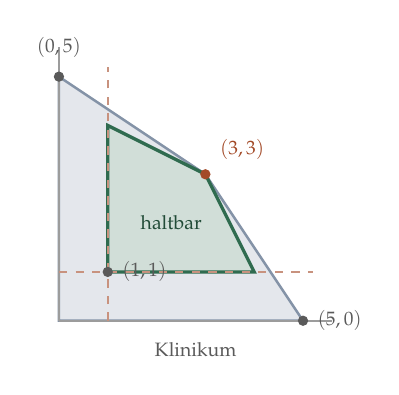
\begin{tikzpicture}[scale=0.62]
\fill[tief!12] (3,3) -- (5,0) -- (0,0) -- (0,5) -- cycle;
\draw[tief!55, line width=0.9pt] (3,3) -- (5,0) -- (0,0) -- (0,5) -- cycle;
\fill[gruen!22] (3,3) -- (4,1) -- (1,1) -- (1,4) -- cycle;
\draw[gruen, line width=1.2pt] (3,3) -- (4,1) -- (1,1) -- (1,4) -- cycle;
\draw[grau!60, line width=0.6pt] (0,0) -- (5.6,0);
\draw[grau!60, line width=0.6pt] (0,0) -- (0,5.6);
\draw[akzent!60, line width=0.7pt, dashed] (1,0) -- (1,5.2);
\draw[akzent!60, line width=0.7pt, dashed] (0,1) -- (5.2,1);
\fill[akzent] (3,3) circle (3pt); \fill[grau] (1,1) circle (3pt);
\fill[grau] (5,0) circle (3pt); \fill[grau] (0,5) circle (3pt);
\node[font=\scriptsize, color=akzent, anchor=south west] at (3.1,3.1) {$(3,3)$};
\node[font=\scriptsize, color=grau, anchor=south west] at (1.1,0.6) {$(1,1)$};
\node[font=\scriptsize, color=grau, anchor=west] at (5.1,0) {$(5,0)$};
\node[font=\scriptsize, color=grau, anchor=south] at (0,5.2) {$(0,5)$};
\node[font=\scriptsize, color=gruen!70!black] at (2.3,2.0) {haltbar};
\node[font=\scriptsize, color=grau] at (2.8,-0.6) {Klinikum};
\end{tikzpicture}
\end{center}

\begin{center}
\begin{minipage}{0.9\textwidth}
\textbf{Jeder Punkt im grünen Bereich ist ein Gleichgewicht --- bei hinreichender Geduld.}
\end{minipage}
\end{center}
\end{merksatz}

\begin{warnung}
\boxtitelr{Was der Volkssatz kostet}
\begin{center}
\begin{minipage}{0.9\textwidth}
\textbf{Ein Vorhersagebegriff, der fast alles zulässt, sagt fast nichts vorher.}
\end{minipage}
\end{center}

\begin{center}
{\small
\renewcommand{\arraystretch}{1.5}
\begin{tabular}{@{}P{2.4cm}P{6.2cm}@{}}
\toprule
\textbf{Die gute Seite} & Zusammenarbeit ist erklärbar, ohne Altruismus zu unterstellen.\\
\textbf{Die schlechte} & Auch $(1{,}1;\ 4{,}5)$ ist ein Gleichgewicht --- und $(3,3)$ und $(1,1)$ und ein Kontinuum dazwischen.\\
\bottomrule
\end{tabular}}
\end{center}

\begin{center}
\begin{minipage}{0.88\textwidth}
\kursiv{Der Name ist bezeichnend: \enquote{Volkssatz} heißt, dass das Ergebnis lange mündlich weitergegeben wurde, ohne dass jemand es veröffentlichte oder für sich beanspruchte. \textbf{Man hielt es für zu einfach und zu wenig aussagekräftig zugleich.} Erst Aumann und Shapley (1976) sowie Fudenberg und Maskin (1986) gaben präzise Fassungen.}
\end{minipage}
\end{center}

\schritt{Die Folge für die Praxis}
\begin{center}
\begin{minipage}{0.88\textwidth}
\kursiv{Wer eine wiederholte Anreizlage gestalten will, kann sich nicht auf den Satz stützen --- er sagt nur, dass gute Lösungen \kursiv{möglich} sind. \textbf{Welche eintritt, entscheidet sich außerhalb des Modells}: durch Vorgeschichte, Absprache, Gewohnheit. Kapitel~10 gibt eine der wenigen Antworten, die innerhalb der Theorie bleiben.}
\end{minipage}
\end{center}
\end{warnung}

\section{Der Bruchfall}

\begin{warnung}
\boxtitelr{Was Fehler anrichten}
Kein Beobachtungssystem ist vollkommen. Eine Resistenzstatistik kann eine Zurückhaltung als Ausscheren ausweisen.

\schritt{Grimm bei einem Fehler}
\begin{center}
\begin{minipage}{0.9\textwidth}
\textbf{Ein einziger falscher Befund zerstört die Zusammenarbeit für immer.}
\end{minipage}
\end{center}

\schritt{Tit for Tat bei einem Fehler}
\begin{center}
{\small
\renewcommand{\arraystretch}{1.44}
\begin{tabular}{@{}P{1.4cm}P{1.8cm}P{1.8cm}P{2.4cm}@{}}
\toprule
\textbf{Runde} & \textbf{K} & \textbf{M} & \\
\midrule
$1$ & zurück & zurück & \\
$2$ & zurück & \textcolor{akzent}{frei} & Fehler\\
$3$ & \textcolor{akzent}{frei} & zurück & \\
$4$ & zurück & \textcolor{akzent}{frei} & \\
$5$ & \textcolor{akzent}{frei} & zurück & \\
\bottomrule
\end{tabular}}
\end{center}

\begin{center}
\begin{minipage}{0.9\textwidth}
\textbf{Ein Echo, das nie abklingt.} Beide erhalten im Mittel $\tfrac{5+0}{2} = 2{,}5$ statt $3$.
\end{minipage}
\end{center}

\begin{center}
\begin{minipage}{0.88\textwidth}
\kursiv{Und ein \kursiv{zweiter} Fehler kann das Echo beenden --- oder in dauerhaftes beidseitiges Ausscheren überführen, je nachdem, wann er auftritt. \textbf{Tit for Tat ist gegen Fehler nicht robust}, obwohl es in Axelrods fehlerfreiem Turnier gewann.}
\end{minipage}
\end{center}

\schritt{Die Abhilfe}
\begin{center}
{\small
\renewcommand{\arraystretch}{1.5}
\begin{tabular}{@{}P{2.6cm}P{6.0cm}@{}}
\toprule
\textbf{Großzügig} & Vergilt nur mit einer Wahrscheinlichkeit von etwa $0{,}9$ --- das Echo bricht ab.\\
\textbf{Zwei Vergehen} & Vergilt erst nach zweimaligem Ausscheren.\\
\textbf{Gewinnen-bleiben} & Ändert die Strategie nur, wenn die letzte Runde schlecht lief.\\
\bottomrule
\end{tabular}}
\end{center}

\begin{center}
\begin{minipage}{0.88\textwidth}
\kursiv{In Turnieren mit Rauschen schlagen alle drei das reine Tit for Tat. \textbf{Die dritte Zeile hat sich als besonders widerstandsfähig erwiesen}: Sie kooperiert nach gegenseitigem Zurückhalten, schert nach beidseitigem Ausscheren wieder ein --- und beutet einen Gegner aus, der dauerhaft nachgibt. Damit ist sie nicht mehr \enquote{nett} im Sinne Axelrods.}
\end{minipage}
\end{center}
\end{warnung}

\section{Übungsaufgaben}

\begin{aufgabe}
\boxtitel{Aufgabe 8.1 --- Die Schwelle bestimmen}
Wie ändert sich die Grimm-Schwelle, wenn die Versuchung $T$ steigt? Rechnen Sie für $T = 4$, $6$, $10$ bei $R=3$, $P=1$.

\loesung
\schritt{Schritt 1 --- Die Formel}
\[ \delta^{*} = \frac{T-R}{T-P} \]

\schritt{Schritt 2 --- Die Werte}
\begin{center}
{\small
\renewcommand{\arraystretch}{1.5}
\begin{tabular}{@{}P{1.4cm}P{2.4cm}P{1.8cm}P{2.2cm}@{}}
\toprule
$T$ & \textbf{Rechnung} & $\delta^{*}$ & \textbf{Runden}\\
\midrule
$4$ & $\tfrac{1}{3}$ & $0{,}333$ & $1{,}5$\\
$5$ & $\tfrac{2}{4}$ & $0{,}500$ & $2{,}0$\\
$6$ & $\tfrac{3}{5}$ & $0{,}600$ & $2{,}5$\\
$10$ & $\tfrac{7}{9}$ & $0{,}778$ & $4{,}5$\\
\bottomrule
\end{tabular}}
\end{center}

\schritt{Schritt 3 --- Der Grenzwert}
\[ \lim_{T\to\infty} \frac{T-R}{T-P} = 1 \]

\begin{center}
\begin{minipage}{0.9\textwidth}
\textbf{Die Schwelle steigt, erreicht aber nie eins.} Zu jeder noch so großen Versuchung gibt es eine Geduld, die sie aushält.
\end{minipage}
\end{center}

\schritt{Schritt 4 --- Die Gegenprobe mit Tit for Tat}
\[ \delta^{*} = \frac{T-R}{R} \]
\begin{center}
{\small
\renewcommand{\arraystretch}{1.5}
\begin{tabular}{@{}P{1.4cm}P{2.0cm}P{2.0cm}P{2.2cm}@{}}
\toprule
$T$ & \textbf{Grimm} & \textbf{Tit for Tat} & \\
\midrule
$4$ & $0{,}333$ & $0{,}333$ & gleich\\
$5$ & $0{,}500$ & $0{,}667$ & \\
$6$ & $0{,}600$ & $1{,}000$ & \textcolor{mittel}{Grenzfall}\\
$10$ & $0{,}778$ & $2{,}333$ & \textcolor{akzent}{unmöglich}\\
\bottomrule
\end{tabular}}
\end{center}

\begin{center}
\begin{minipage}{0.9\textwidth}
\textbf{Ab $T > 2R - R = 6$ kann Tit for Tat die Zusammenarbeit gar nicht mehr tragen --- Grimm sehr wohl.}
\end{minipage}
\end{center}

\begin{center}
\begin{minipage}{0.88\textwidth}
\kursiv{Die Bedingung lautet $T \le 2R$, denn $\frac{T-R}{R} \le 1$ ist gleichbedeutend mit $T \le 2R$. \textbf{Sie ist genau die Bedingung dafür, dass abwechselndes Ausbeuten nicht besser ist als beidseitiges Zurückhalten} --- und sie erscheint in der Turnierliteratur regelmäßig als Zusatzforderung an die Auszahlungen, meist ohne Begründung.}
\end{minipage}
\end{center}
\end{aufgabe}

\begin{aufgabe}
\boxtitel{Aufgabe 8.2 --- Endlich und unendlich}
Das Marienhospital kündigt an, in fünf Jahren zu fusionieren --- das Spiel endet dann. Was folgt daraus, und was ändert eine Unsicherheit über den Zeitpunkt?

\loesung
\schritt{Schritt 1 --- Mit bekanntem Ende}
Nach Satz 8.1 schert beidseitig ab der ersten Runde aus.

\begin{center}
\renewcommand{\arraystretch}{1.48}
\begin{tabular}{@{}P{2.4cm}P{2.4cm}P{2.4cm}@{}}
\toprule
\textbf{Jahr} & \textbf{Verhalten} & \textbf{Ertrag}\\
\midrule
$1$ bis $5$ & beide frei & $1$ je Jahr\\
\midrule
\textbf{Summe} & & $\mathbf{5}$\\
\bottomrule
\end{tabular}
\end{center}

\schritt{Schritt 2 --- Die Bilanz des Verzichts}
Bei Zusammenarbeit über fünf Jahre:
\[ 5\cdot3 = 15 \]

\begin{center}
\begin{minipage}{0.9\textwidth}
\textbf{Zehn Einheiten gehen verloren --- wegen einer Ankündigung.}
\end{minipage}
\end{center}

\schritt{Schritt 3 --- Mit unsicherem Ende}
Endet das Spiel in jedem Jahr mit Wahrscheinlichkeit $0{,}2$, so ist $\delta = 0{,}8$.

\[ 0{,}8 \ \ge\ \tfrac12 \quad \checkmark \]

Grimm trägt. Die erwartete Zusammenarbeit bringt
\[ \frac{3}{1-0{,}8} = 15 \]

\begin{center}
\begin{minipage}{0.9\textwidth}
\textbf{Dieselbe erwartete Dauer von fünf Jahren --- aber Zusammenarbeit statt Ausscheren.}
\end{minipage}
\end{center}

\kursiv{Probe der Dauer:} $\frac{1}{1-0{,}8} = 5$ \checkmark

\schritt{Schritt 4 --- Die Lehre}
\begin{center}
{\small
\renewcommand{\arraystretch}{1.5}
\begin{tabular}{@{}P{2.6cm}P{2.0cm}P{2.6cm}@{}}
\toprule
& \textbf{Dauer} & \textbf{Ertrag}\\
\midrule
sicher $5$ Jahre & $5$ & $5$\\
erwartet $5$ Jahre & $5$ & $\mathbf{15}$\\
\bottomrule
\end{tabular}}
\end{center}

\begin{center}
\begin{minipage}{0.88\textwidth}
\kursiv{\textbf{Die Ungewissheit über das Ende ist wertvoller als eine längere sichere Dauer.} Das ist eines der wenigen Ergebnisse dieses Bandes, die eine unmittelbare Handlungsanweisung enthalten: Wer eine Zusammenarbeit erhalten will, sollte kein Enddatum bekanntgeben. Gekündigte Verträge verlieren ihre Bindungskraft lange vor dem Ablauf.}
\end{minipage}
\end{center}

\schritt{Schritt 5 --- Der Vorbehalt}
\begin{center}
\begin{minipage}{0.88\textwidth}
\kursiv{Satz 8.1 ist empirisch ebenso schlecht bestätigt wie das Tausendfüßlerspiel: In Versuchen mit bekanntem Ende kooperieren die meisten Teilnehmer bis kurz vor Schluss und scheren erst in den letzten ein bis zwei Runden aus. \textbf{Der Zusammenbruch geschieht am Ende, nicht am Anfang} --- was die Rückwärtsinduktion gerade nicht vorhersagt.}
\end{minipage}
\end{center}
\end{aufgabe}

\begin{aufgabe}
\boxtitel{Aufgabe 8.3 --- Ein Fehler und seine Folgen}
Beide Häuser spielen Tit for Tat. In Runde 2 wird die Zurückhaltung des Marienhospitals fälschlich als Ausscheren gemeldet. Berechnen Sie den Verlust über zwanzig Runden.

\loesung
\schritt{Schritt 1 --- Der Verlauf}
\begin{center}
{\small
\renewcommand{\arraystretch}{1.44}
\begin{tabular}{@{}P{1.6cm}P{1.6cm}P{1.6cm}P{2.4cm}@{}}
\toprule
\textbf{Runde} & \textbf{K} & \textbf{M} & \textbf{Auszahlung K}\\
\midrule
$1$ & zurück & zurück & $3$\\
$2$ & zurück & zurück\textsuperscript{*} & $3$\\
$3$ & frei & zurück & $5$\\
$4$ & zurück & frei & $0$\\
$5$ & frei & zurück & $5$\\
$6$ & zurück & frei & $0$\\
\bottomrule
\end{tabular}}
\end{center}
\kursiv{\textsuperscript{*}als Ausscheren gemeldet}

\schritt{Schritt 2 --- Der Mittelwert ab Runde 3}
\[ \frac{5+0}{2} = 2{,}5 \ \text{je Runde} \]

\schritt{Schritt 3 --- Die Bilanz}
\begin{center}
{\small
\renewcommand{\arraystretch}{1.5}
\begin{tabular}{@{}P{2.6cm}P{2.4cm}P{2.4cm}@{}}
\toprule
& \textbf{ohne Fehler} & \textbf{mit Fehler}\\
\midrule
Runden $1$--$2$ & $6$ & $6$\\
Runden $3$--$20$ & $54$ & $45$\\
\midrule
\textbf{Summe} & $\mathbf{60}$ & $\mathbf{51}$\\
\bottomrule
\end{tabular}}
\end{center}

\[ \text{Verlust} = 9 \ \text{Einheiten}, \ \text{also } 15\,\% \]

\schritt{Schritt 4 --- Mit Grimm statt Tit for Tat}
\begin{center}
\renewcommand{\arraystretch}{1.48}
\begin{tabular}{@{}P{2.6cm}P{2.2cm}P{2.6cm}@{}}
\toprule
\textbf{Strategie} & \textbf{Ertrag} & \textbf{Verlust}\\
\midrule
ohne Fehler & $60$ & --- \\
Tit for Tat & $51$ & $15\,\%$\\
Grimm & $24$ & $\mathbf{60\,\%}$\\
\bottomrule
\end{tabular}
\end{center}

\kursiv{Zu Grimm:} $2\cdot3 + 18\cdot1 = 6+18 = 24$.

\begin{center}
\begin{minipage}{0.9\textwidth}
\textbf{Die härtere Strategie hat die niedrigere Schwelle und den größeren Fehlerschaden.}
\end{minipage}
\end{center}

\schritt{Schritt 5 --- Großzügiges Tit for Tat}
Die Strategie vergilt nur mit Wahrscheinlichkeit $0{,}9$. Die erwartete Dauer des Echos beträgt
\[ \frac{1}{1-0{,}9} = 10 \ \text{Runden}, \]
davon die Hälfte mit Ertrag $5$ und die Hälfte mit $0$.

\kursiv{Erwarteter Verlust gegenüber durchgehender Zusammenarbeit:}
\[ 10\cdot(3 - 2{,}5) = 5 \ \text{Einheiten} \]

\begin{center}
{\small
\renewcommand{\arraystretch}{1.5}
\begin{tabular}{@{}P{2.8cm}P{2.0cm}P{2.4cm}@{}}
\toprule
\textbf{Strategie} & \textbf{Verlust} & \\
\midrule
Grimm & $36$ & $\delta^{*}=0{,}50$\\
Tit for Tat & $9$ & $\delta^{*}=0{,}67$\\
großzügig & $\mathbf{5}$ & etwas höher\\
\bottomrule
\end{tabular}}
\end{center}

\schritt{Schritt 6 --- Der Zielkonflikt}
\begin{center}
\begin{minipage}{0.88\textwidth}
\kursiv{\textbf{Härte senkt die Geduldsschwelle und erhöht die Fehlerkosten.} Welche Strategie besser ist, hängt davon ab, wie verlässlich beobachtet wird --- eine Frage, die in der Matrix nicht vorkommt. Bei guter Beobachtung wählt man Grimm, bei schlechter eine großzügige Variante. Dieselbe Abwägung erscheint in Band 20, Kapitel~6 als Wahl zwischen Fehlererkennung und Fehlerkorrektur.}
\end{minipage}
\end{center}
\end{aufgabe}

\begin{geschichte}
\boxtitelg{Ein Turnier mit vierzehn Teilnehmern}
\Person{Robert Axelrod} (geboren 1943), Politikwissenschaftler in Michigan, lud 1979 Fachleute ein, Strategien für ein wiederholtes Gefangenendilemma einzureichen.

\begin{center}
\begin{minipage}{0.9\textwidth}
\kursiv{Vierzehn Beiträge gingen ein, aus Wirtschaftswissenschaft, Psychologie, Mathematik und Informatik. Jede Strategie spielte gegen jede zweihundert Runden. \textbf{Die kürzeste gewann}: Tit for Tat, eingereicht von \Person{Anatol Rapoport}, fünf Zeilen Fortran.}
\end{minipage}
\end{center}

\schritt{Das zweite Turnier}
Axelrod veröffentlichte die Ergebnisse vollständig und lud erneut ein. Dreiundsechzig Beiträge kamen, viele eigens gegen Tit for Tat entworfen.

\begin{center}
\begin{minipage}{0.9\textwidth}
\kursiv{Rapoport reichte dieselben fünf Zeilen ein und gewann wieder. \textbf{Das ist das bemerkenswertere Ergebnis} --- denn diesmal kannten alle Teilnehmer den Sieger und hatten ein Jahr Zeit, ihn zu schlagen.}
\end{minipage}
\end{center}

\schritt{Die vier Eigenschaften}
Axelrod fasste zusammen, was erfolgreiche Strategien auszeichnete:

\begin{center}
{\small
\renewcommand{\arraystretch}{1.5}
\begin{tabular}{@{}P{2.8cm}P{5.8cm}@{}}
\toprule
\textbf{nett} & schert nie als erste aus\\
\textbf{vergeltend} & lässt Ausscheren nicht durchgehen\\
\textbf{versöhnlich} & kehrt rasch zur Zusammenarbeit zurück\\
\textbf{durchschaubar} & ist für den Gegner leicht zu erkennen\\
\bottomrule
\end{tabular}}
\end{center}

\begin{center}
\begin{minipage}{0.9\textwidth}
\kursiv{\textbf{Die vierte Eigenschaft überrascht am meisten.} In einem Nullsummenspiel wäre Durchschaubarkeit tödlich --- Kapitel~2. Hier ist sie nützlich, weil der Gegner erkennen können muss, dass Zusammenarbeit belohnt wird. Der Unterschied zwischen Teil~I und Teil~III liegt in diesem einen Punkt.}
\end{minipage}
\end{center}

\schritt{Die späteren Einschränkungen}
Ab den 1990er Jahren zeigten Turniere mit Rauschen, dass Tit for Tat dort deutlich schlechter abschneidet.

\begin{center}
\begin{minipage}{0.9\textwidth}
\kursiv{2004 gewann ein Turnier eine Gruppe aus Southampton, die mehrere Strategien einreichte, die sich gegenseitig an einem Erkennungsmuster identifizierten und dann eine davon zum Sieg fütterten. \textbf{Das war regelkonform und hat die Turnierform als Erkenntnisquelle beschädigt} --- ein Turnier misst, was man einreichen darf, nicht was sich bewährt.}
\end{minipage}
\end{center}
\end{geschichte}

\begin{forschung}
\boxtitelp{Wiederholung heute}
\begin{center}
{\small
\renewcommand{\arraystretch}{1.45}
\begin{tabular}{@{}P{2.8cm}P{5.4cm}@{}}
\toprule
\textbf{Unvollkommene Beobachtung} & Wenn niemand sicher weiß, was der andere tat --- die realistische Lage.\\
\textbf{Ruf} & Zusammenarbeit zwischen Fremden über Dritte, die berichten.\\
\textbf{Gestaltung} & Wie man Wiederholung bewusst herstellt.\\
\bottomrule
\end{tabular}}
\end{center}

\schritt{Zur ersten Zeile}
Beobachtet jeder nur ein verrauschtes Signal, so lässt sich die Zusammenarbeit nicht mehr vollständig aufrechterhalten.

\begin{center}
\begin{minipage}{0.88\textwidth}
\kursiv{\Person{Green} und \Person{Porter} zeigten 1984 an einem Kartellmodell, dass Gleichgewichte notwendig Strafphasen enthalten, in denen niemand geschummelt hat --- man bestraft ein schlechtes Signal, nicht eine Tat. \textbf{Preiskriege wären danach kein Zusammenbruch des Kartells, sondern Teil seiner Funktionsweise.} Das Ergebnis hat die Kartellermittlung verändert.}
\end{minipage}
\end{center}

\schritt{Zur dritten Zeile}
\begin{center}
\begin{minipage}{0.88\textwidth}
\kursiv{Im Leitfall bedeutet das: Man richtet regelmäßige gemeinsame Resistenzkonferenzen ein, veröffentlicht die Verschreibungsdaten und sorgt dafür, dass die Zusammenarbeit kein absehbares Ende hat. \textbf{Alle drei Maßnahmen verändern nicht die Auszahlungen, sondern $\delta$ und die Beobachtbarkeit} --- und sind damit billiger als die Anreizänderung aus Kapitel~5.}
\end{minipage}
\end{center}
\end{forschung}

\begin{merksatz}
\boxtitel{Was Sie jetzt können}
\begin{center}
\renewcommand{\arraystretch}{1.5}
\begin{tabular}{@{}P{3.0cm}P{5.6cm}@{}}
\toprule
\textbf{Satz 8.1} & bekanntes Ende zerstört alles\\
\textbf{Satz 8.2} & $\delta \ge (T-R)/(T-P)$\\
\textbf{Tit for Tat} & $\delta \ge (T-R)/R$, milder und geduldiger\\
\textbf{Satz 8.3} & Volkssatz: fast alles ist möglich\\
\textbf{Der Bruchfall} & Härte senkt die Schwelle, erhöht den Fehlerschaden\\
\bottomrule
\end{tabular}
\end{center}

\begin{center}
\begin{minipage}{0.88\textwidth}
\kursiv{Damit endet Teil~III. Bisher haben die Spieler nachgedacht. Ab Kapitel~9 tun sie es nicht mehr --- und dieselben Gleichgewichte stellen sich trotzdem ein.}
\end{minipage}
\end{center}
\end{merksatz}

\part{Evolution}

\chapter{Evolutionär stabile Strategien}

\section{Spieler, die nicht nachdenken}

\begin{merksatz}
\boxtitel{Die Voraussetzungen fallen weg}
Alle bisherigen Kapitel setzten voraus, dass Spieler die Auszahlungen kennen, rechnen können und Erwartungen über andere bilden.

\begin{center}
{\small
\renewcommand{\arraystretch}{1.5}
\begin{tabular}{@{}P{2.4cm}P{6.2cm}@{}}
\toprule
\textbf{Kapitel 1} & Allgemeines Wissen über die Auszahlungen.\\
\textbf{Kapitel 4} & Nutzenfunktionen im Sinne von Satz 4.1.\\
\textbf{Kapitel 7} & Glaube an die Rationalität aller anderen.\\
\bottomrule
\end{tabular}}
\end{center}

\begin{center}
\begin{minipage}{0.9\textwidth}
\textbf{Bakterien erfüllen keine dieser Bedingungen --- und stellen dennoch Gleichgewichte her.}
\end{minipage}
\end{center}

\begin{center}
\begin{minipage}{0.88\textwidth}
\kursiv{Das ist der Befund, der Teil~IV trägt. Was im ersten Teil des Bandes eine Annahme über Denkleistung war, wird hier zu einer Aussage über Vermehrung: \textbf{Wer mehr Nachkommen hinterlässt, breitet sich aus} --- und das genügt. Die Auszahlung heißt nun \Begriff{Eignung} und misst den Fortpflanzungserfolg.}
\end{minipage}
\end{center}
\end{merksatz}

\begin{merksatz}
\boxtitel{Der Leitfall: zwei Stämme im Darm}
Ein Patient trägt zwei Stämme desselben Bakteriums. Der eine bildet Giftstoffe, die konkurrierende Zellen abtöten --- das kostet Stoffwechselleistung. Der andere bildet keine.

\begin{center}
{\small
\renewcommand{\arraystretch}{1.5}
\begin{tabular}{@{}P{2.2cm}P{6.4cm}@{}}
\toprule
\textbf{Falke} & bildet Giftstoffe, kämpft um die Nische\\
\textbf{Taube} & teilt sich die Nische, weicht aus\\
\bottomrule
\end{tabular}}
\end{center}

\begin{center}
{\small
\renewcommand{\arraystretch}{1.5}
\begin{tabular}{@{}P{2.0cm}P{2.8cm}P{2.8cm}@{}}
\toprule
\textbf{Treffen} & \textbf{Ergebnis} & \textbf{Eignung}\\
\midrule
Falke--Falke & Kampf, beide geschädigt & $\tfrac{V-C}{2}$\\
Falke--Taube & Falke nimmt alles & $V$ bzw.\ $0$\\
Taube--Taube & geteilt & $\tfrac{V}{2}$\\
\bottomrule
\end{tabular}}
\end{center}

\kursiv{Mit $V = 2$ (die Nische) und $C = 4$ (die Kosten des Kampfes):}
\begin{center}
{\small
\renewcommand{\arraystretch}{1.6}
\begin{tabular}{@{}P{2.0cm}P{2.2cm}P{2.2cm}@{}}
\toprule
& \textbf{Falke} & \textbf{Taube}\\
\midrule
\textbf{Falke} & $-1$ & $2$\\
\textbf{Taube} & $0$ & $1$\\
\bottomrule
\end{tabular}}
\end{center}

\begin{center}
\begin{minipage}{0.88\textwidth}
\kursiv{Nur eine Matrix --- denn beide Stämme spielen dasselbe Spiel und haben dieselben Aussichten. \textbf{Solche Spiele heißen symmetrisch}, und die Evolutionstheorie kennt fast nur diese: Ein Gen hat keine Sonderrolle, es trifft auf Kopien seiner selbst und auf Konkurrenten.}
\end{minipage}
\end{center}

\begin{center}
\begin{minipage}{0.88\textwidth}
\kursiv{Man erkennt die Ordnung $T=2 > R=1 > S=0 > P=-1$ --- das ist das Feigheitsspiel aus Kapitel~5. \textbf{Dieselbe Struktur, ein völlig anderer Zugang} zur Lösung.}
\end{minipage}
\end{center}
\end{merksatz}

\section{Die Definition}

\begin{definition}
\boxtitelm{Definition 9.1 --- evolutionär stabil}
Eine Strategie $\sigma^{*}$ heißt \Begriff{evolutionär stabil}, wenn für jede andere Strategie $\sigma$ gilt:
\begin{center}
{\small
\renewcommand{\arraystretch}{1.55}
\begin{tabular}{@{}P{1.0cm}P{7.4cm}@{}}
\toprule
(i) & $\Aus(\sigma^{*},\sigma^{*}) > \Aus(\sigma,\sigma^{*})$, \quad oder\\
(ii) & $\Aus(\sigma^{*},\sigma^{*}) = \Aus(\sigma,\sigma^{*})$ \ und \ $\Aus(\sigma^{*},\sigma) > \Aus(\sigma,\sigma)$.\\
\bottomrule
\end{tabular}}
\end{center}
\end{definition}

\begin{merksatz}
\boxtitel{Was die beiden Bedingungen bedeuten}
Man stelle sich eine Bevölkerung vor, die durchweg $\sigma^{*}$ spielt. Ein kleiner Anteil $\varepsilon$ von Abweichlern spielt $\sigma$.

\begin{center}
{\small
\renewcommand{\arraystretch}{1.5}
\begin{tabular}{@{}P{2.0cm}P{6.6cm}@{}}
\toprule
\textbf{(i)} & Der Abweichler schneidet schon gegen die Mehrheit schlechter ab --- er verschwindet.\\
\textbf{(ii)} & Er ist gegen die Mehrheit gleich gut. Dann entscheidet, wie beide gegen \kursiv{ihn} abschneiden --- und dort muss $\sigma^{*}$ besser sein.\\
\bottomrule
\end{tabular}}
\end{center}

\schritt{Die Rechnung dahinter}
In einer Bevölkerung mit Anteil $\varepsilon$ Abweichlern trifft man mit $1-\varepsilon$ auf $\sigma^{*}$ und mit $\varepsilon$ auf $\sigma$:
\begin{align*}
\Aus(\sigma^{*}) &= (1-\varepsilon)\,\Aus(\sigma^{*},\sigma^{*}) + \varepsilon\,\Aus(\sigma^{*},\sigma)\\
\Aus(\sigma) &= (1-\varepsilon)\,\Aus(\sigma,\sigma^{*}) + \varepsilon\,\Aus(\sigma,\sigma)
\end{align*}

\begin{center}
\begin{minipage}{0.9\textwidth}
\textbf{Für kleines $\varepsilon$ überwiegt der erste Summand.} Ist er gleich, so entscheidet der zweite --- genau die Fallunterscheidung der Definition.
\end{minipage}
\end{center}

\begin{center}
\begin{minipage}{0.88\textwidth}
\kursiv{Die Definition ist also keine Willkür, sondern die Auswertung einer Ungleichung für hinreichend kleines $\varepsilon$. \textbf{Evolutionäre Stabilität heißt: Eine kleine Abweichlergruppe kann nicht Fuß fassen.} Über große Störungen sagt sie nichts --- ein Vorbehalt, auf den der Bruchfall zurückkommt.}
\end{minipage}
\end{center}
\end{merksatz}

\begin{merksatz}
\boxtitel{Satz 9.2 --- jede stabile Strategie ist ein Gleichgewicht}
Ist $\sigma^{*}$ evolutionär stabil, so ist $(\sigma^{*},\sigma^{*})$ ein Nash-Gleichgewicht.

\schritt{Beweis}
Beide Fälle der Definition liefern
\[ \Aus(\sigma^{*},\sigma^{*}) \ \ge\ \Aus(\sigma,\sigma^{*}) \qquad\text{für alle } \sigma . \]
Das ist genau Definition 4.3 für ein symmetrisches Profil. $\blacksquare$

\schritt{Die Umkehrung gilt nicht}
\[ A = \begin{pmatrix} 2 & 1\\ 1 & 1\end{pmatrix} \]

\kursiv{Für $\sigma^{*} = S_2$:} $\Aus(S_2,S_2) = 1 = \Aus(S_1,S_2)$ --- ein Nash-Gleichgewicht, aber Bedingung (i) scheitert.

\kursiv{Bedingung (ii):} $\Aus(S_2,S_1) = 1$ gegen $\Aus(S_1,S_1) = 2$. Gefordert wäre $1 > 2$.

\begin{center}
\begin{minipage}{0.9\textwidth}
\textbf{$S_2$ ist ein Nash-Gleichgewicht und nicht evolutionär stabil.} Abweichler zu $S_1$ verlieren nichts und gewinnen, sobald sie sich begegnen.
\end{minipage}
\end{center}

\begin{center}
\begin{minipage}{0.88\textwidth}
\kursiv{Evolutionäre Stabilität ist also eine \kursiv{Verfeinerung} des Gleichgewichtsbegriffs --- eine weitere neben der Teilspielperfektheit aus Kapitel~7. \textbf{Sie schließt genau die schwachen Gleichgewichte aus}, bei denen ein Abweichen nichts kostet. Und sie tut es aus einem völlig anderen Grund: nicht wegen Glaubwürdigkeit, sondern wegen Vermehrung.}
\end{minipage}
\end{center}
\end{merksatz}

\section{Der Leitfall gelöst}

\begin{merksatz}
\boxtitel{Keine reine Strategie ist stabil}
\kursiv{Falke:} $\Aus(F,F) = -1$, $\Aus(T,F) = 0$. Also $-1 < 0$ --- Bedingung (i) scheitert, und (ii) auch, denn die Werte sind nicht gleich.

\begin{center}
\begin{minipage}{0.9\textwidth}
\textbf{In einer reinen Falkenbevölkerung fahren Tauben besser.} Sie kämpfen nicht und verlieren nichts.
\end{minipage}
\end{center}

\kursiv{Taube:} $\Aus(T,T) = 1$, $\Aus(F,T) = 2$. Also $1 < 2$.

\begin{center}
\begin{minipage}{0.9\textwidth}
\textbf{In einer reinen Taubenbevölkerung fahren Falken besser.} Sie nehmen alles.
\end{minipage}
\end{center}

\schritt{Die gemischte Strategie}
Nach dem Prinzip aus Satz 3.3 ist $p$ so zu wählen, dass beide Typen gleich gut fahren:
\[ p\cdot(-1) + (1-p)\cdot2 = p\cdot0 + (1-p)\cdot1 \]
\[ 2-3p = 1-p \quad\Longrightarrow\quad 1 = 2p \quad\Longrightarrow\quad p = \tfrac12 \]

\schritt{Die allgemeine Formel}
\[ p\cdot\frac{V-C}{2} + (1-p)\,V = (1-p)\,\frac{V}{2} \]
führt auf
\[ \boxed{\ p^{*} = \frac{V}{C}\ } \qquad\text{für } V < C \]

\schritt{Die Eignung im Gleichgewicht}
\[ \Aus^{*} = (1-p^{*})\,\frac{V}{2} = \left(1-\frac VC\right)\frac V2 = \frac{V\,(C-V)}{2C} \]

\kursiv{Im Leitfall:} $\frac{2\cdot2}{8} = \tfrac12$ \checkmark

\begin{center}
{\small
\renewcommand{\arraystretch}{1.48}
\begin{tabular}{@{}P{1.4cm}P{1.4cm}P{1.8cm}P{2.2cm}@{}}
\toprule
$V$ & $C$ & $p^{*}$ & \textbf{Eignung}\\
\midrule
$2$ & $3$ & $0{,}667$ & $0{,}333$\\
$2$ & $4$ & $0{,}500$ & $0{,}500$\\
$2$ & $8$ & $0{,}250$ & $0{,}750$\\
$4$ & $2$ & $1{,}000$ & $1{,}000$\\
\bottomrule
\end{tabular}}
\end{center}

\begin{center}
\begin{minipage}{0.9\textwidth}
\textbf{Je teurer der Kampf, desto seltener wird gekämpft --- und desto besser fahren alle.}
\end{minipage}
\end{center}

\begin{center}
\begin{minipage}{0.88\textwidth}
\kursiv{Die dritte Zeile ist der bemerkenswerte Fall: Bei achtfachen Kampfkosten erreichen alle eine Eignung von $0{,}75$, während die friedliche Teilung nur $1$ brächte --- der Verlust beträgt nur ein Viertel. \textbf{Hohe Strafen für Aggression bringen eine Bevölkerung nahe an das friedliche Ergebnis}, ohne dass jemand friedlich sein müsste. Das ist die evolutionäre Entsprechung zu Aufgabe 5.1.}
\end{minipage}
\end{center}

\schritt{Der Fall $V \ge C$}
\begin{center}
\begin{minipage}{0.9\textwidth}
\textbf{Ist die Nische mehr wert als der Kampf kostet, so ist Falke strikt dominant und die einzige stabile Strategie.}
\end{minipage}
\end{center}

\kursiv{Denn dann ist $\frac{V-C}{2} \ge 0$ und $V > \frac{V}{2}$.} Aus dem Feigheitsspiel wird ein Spiel mit dominanter Strategie.
\end{merksatz}

\begin{merksatz}
\boxtitel{Was das erklärt}
\begin{center}
{\small
\renewcommand{\arraystretch}{1.5}
\begin{tabular}{@{}P{2.4cm}P{6.2cm}@{}}
\toprule
\textbf{Ritualkämpfe} & Viele Arten tragen Rangkämpfe aus, ohne einander zu töten --- hohe $C$ halten $p^{*}$ klein.\\
\textbf{Waffen} & Wer besser bewaffnet ist, hat oft \kursiv{mehr} Hemmungen; $C$ steigt mit der Bewaffnung.\\
\textbf{Mischung} & Die Bevölkerung ist im Gleichgewicht gemischt --- entweder aus zwei Typen oder aus Individuen, die selbst würfeln.\\
\bottomrule
\end{tabular}}
\end{center}

\begin{center}
\begin{minipage}{0.88\textwidth}
\kursiv{Die dritte Zeile ist wichtig und oft missverstanden. \textbf{Das Modell unterscheidet nicht zwischen einer Bevölkerung aus $50$ Prozent Falken und einer aus lauter Individuen, die zur Hälfte aggressiv reagieren.} Beide haben dieselben Eignungswerte. Erst Kapitel~10 kann die Fälle trennen, weil die Dynamik sich unterscheidet.}
\end{minipage}
\end{center}

\begin{center}
\begin{minipage}{0.88\textwidth}
\kursiv{Und die zweite Zeile widerspricht einer verbreiteten Erwartung. \Person{Konrad Lorenz} erklärte Tötungshemmungen mit dem Nutzen für die Art --- ein Argument, das die Evolutionstheorie nicht trägt, weil Selektion an Individuen ansetzt. \textbf{Das Falke-Taube-Modell liefert dieselbe Vorhersage ohne Artnutzen}, allein aus den Kosten für den Einzelnen. Das war 1973 der eigentliche Fortschritt.}
\end{minipage}
\end{center}
\end{merksatz}

\section{Der Bruchfall}

\begin{warnung}
\boxtitelr{Was Definition 9.1 voraussetzt}
\begin{center}
{\small
\renewcommand{\arraystretch}{1.52}
\begin{tabular}{@{}P{2.4cm}P{6.2cm}@{}}
\toprule
\textbf{Unendlich groß} & Die Bevölkerung wird als beliebig groß angenommen; Zufallsschwankungen entfallen.\\
\textbf{Zufällige Paare} & Jeder trifft jeden mit gleicher Wahrscheinlichkeit --- keine Verwandtschaft, keine Nachbarschaft.\\
\textbf{Kleine Störungen} & Stabilität gilt gegen kleine Abweichlergruppen, nicht gegen große.\\
\textbf{Eine Art} & Alle spielen dasselbe Spiel mit denselben Auszahlungen.\\
\bottomrule
\end{tabular}}
\end{center}

\schritt{Zur zweiten Zeile}
Treffen Verwandte häufiger aufeinander, so ändert sich alles.

\begin{center}
\begin{minipage}{0.88\textwidth}
\kursiv{\Person{William Hamilton} zeigte 1964, dass ein Merkmal sich ausbreitet, wenn $r\,b > c$ gilt --- mit $r$ als Verwandtschaftsgrad, $b$ als Nutzen für den anderen und $c$ als eigenen Kosten. \textbf{Bakterienkolonien bestehen weitgehend aus Klonen}, also $r \approx 1$, und dort setzt sich die Zusammenarbeit durch. Im Leitfall heißt das: In einer Monokultur wird nicht gekämpft; Giftstoffbildung lohnt erst beim Zusammentreffen fremder Stämme.}
\end{minipage}
\end{center}

\schritt{Zur ersten Zeile}
Bei kleinen Bevölkerungen kann eine stabile Strategie durch Zufall verschwinden.

\begin{center}
\begin{minipage}{0.88\textwidth}
\kursiv{Die Theorie endlicher Bevölkerungen ergibt teils andere Bedingungen; die Schwelle hängt dann von der Größe ab. \textbf{Bei Bakterien mit $10^{9}$ Zellen ist die Annahme unbedenklich}, bei einer Tierpopulation von fünfzig Individuen nicht.}
\end{minipage}
\end{center}

\schritt{Und eine Stelle, an der es gar kein stabiles Ergebnis gibt}
\begin{center}
\begin{minipage}{0.88\textwidth}
\kursiv{Das zyklische Spiel aus Aufgabe 3.1 --- Stein, Schere, Papier --- hat ein Nash-Gleichgewicht, aber keine evolutionär stabile Strategie. \textbf{Die Bevölkerung kreist dauerhaft}, und das ist kein Rechenfehler, sondern ein beobachtbares Phänomen: Bei einer Eidechsenart mit drei Paarungsstrategien wurde genau ein solcher Kreislauf über Jahre dokumentiert. Kapitel~10 rechnet ihn aus.}
\end{minipage}
\end{center}
\end{warnung}

\section{Übungsaufgaben}

\begin{aufgabe}
\boxtitel{Aufgabe 9.1 --- Die Falkenquote}
Ein Stamm bildet Giftstoffe. Durch eine Antibiotikatherapie steigen die Kosten des Kampfes von $C=4$ auf $C=10$, weil geschädigte Zellen zusätzlich anfällig werden. Was geschieht?

\loesung
\schritt{Schritt 1 --- Die alte Lage}
\[ p^{*} = \frac{V}{C} = \frac{2}{4} = 0{,}50, \qquad \Aus^{*} = \frac{2\cdot2}{8} = 0{,}50 \]

\schritt{Schritt 2 --- Die neue Lage}
\[ p^{*} = \frac{2}{10} = 0{,}20, \qquad \Aus^{*} = \frac{2\cdot8}{20} = 0{,}80 \]

\schritt{Schritt 3 --- Der Vergleich}
\begin{center}
{\small
\renewcommand{\arraystretch}{1.5}
\begin{tabular}{@{}P{1.6cm}P{2.0cm}P{2.0cm}P{2.2cm}@{}}
\toprule
$C$ & \textbf{Falkenanteil} & \textbf{Eignung} & \textbf{Kämpfe}\\
\midrule
$4$ & $50\,\%$ & $0{,}50$ & $25\,\%$\\
$10$ & $20\,\%$ & $0{,}80$ & $4\,\%$\\
\bottomrule
\end{tabular}}
\end{center}

\kursiv{Zu den Kämpfen:} Ein Kampf entsteht nur, wenn zwei Falken aufeinandertreffen --- also mit Wahrscheinlichkeit $(p^{*})^{2}$.

\begin{center}
\begin{minipage}{0.9\textwidth}
\textbf{Die Zahl der Kämpfe sinkt um den Faktor sechs, die mittlere Eignung steigt um sechzig Prozent.}
\end{minipage}
\end{center}

\schritt{Schritt 4 --- Die Grenze}
\[ \lim_{C\to\infty} p^{*} = 0, \qquad \lim_{C\to\infty} \Aus^{*} = \frac{V}{2} \]

\begin{center}
\begin{minipage}{0.9\textwidth}
\textbf{Bei beliebig teuren Kämpfen nähert sich die Bevölkerung dem friedlichen Ergebnis beliebig genau --- erreicht es aber nie.}
\end{minipage}
\end{center}

\begin{center}
\begin{minipage}{0.88\textwidth}
\kursiv{Es bleibt stets ein kleiner Anteil Falken, denn in einer reinen Taubenbevölkerung lohnt sich Aggression immer. \textbf{Das ist der Unterschied zu Aufgabe 5.1}: Dort ließ sich die Dominanz durch einen hinreichend großen Abschlag umkehren; hier verschwindet die Falkenstrategie nie ganz, weil ihr Vorteil gerade bei ihrer Seltenheit am größten ist.}
\end{minipage}
\end{center}

\schritt{Schritt 5 --- Der Vorbehalt}
\begin{center}
\begin{minipage}{0.88\textwidth}
\kursiv{Die Rechnung unterstellt, dass die Therapie nur $C$ verändert und nicht $V$. Tatsächlich verkleinert ein Antibiotikum auch die Nische --- also $V$. \textbf{Sinkt $V$ im selben Verhältnis wie $C$ steigt, so bleibt $p^{*} = V/C$ unverändert}, und die Maßnahme wäre wirkungslos. Welcher Fall vorliegt, ist eine Messfrage und keine Modellfrage.}
\end{minipage}
\end{center}
\end{aufgabe}

\begin{aufgabe}
\boxtitel{Aufgabe 9.2 --- Nash oder stabil?}
Prüfen Sie beide Bedingungen für jede reine Strategie:
\[ A = \begin{pmatrix} 3 & 3\\ 3 & 2\end{pmatrix} \]

\loesung
\schritt{Schritt 1 --- Nash prüfen}
\kursiv{$S_1$:} $\Aus(S_1,S_1) = 3$, $\Aus(S_2,S_1) = 3$. Gleich --- also Nash (schwach).\\
\kursiv{$S_2$:} $\Aus(S_2,S_2) = 2$, $\Aus(S_1,S_2) = 3$. Kleiner --- kein Nash.

\schritt{Schritt 2 --- $S_1$ auf Stabilität prüfen}
\kursiv{Bedingung (i):} $3 > 3$? Nein.

\kursiv{Bedingung (ii):} Der erste Teil ist erfüllt ($3 = 3$). Der zweite verlangt
\[ \Aus(S_1,S_2) > \Aus(S_2,S_2) \]
\[ 3 > 2 \quad \checkmark \]

\begin{center}
\begin{minipage}{0.9\textwidth}
\textbf{$S_1$ ist evolutionär stabil --- über Bedingung (ii).}
\end{minipage}
\end{center}

\schritt{Schritt 3 --- Die Deutung}
\begin{center}
\begin{minipage}{0.88\textwidth}
\kursiv{Ein Abweichler zu $S_2$ verliert zunächst nichts: Gegen die Mehrheit erhält er ebenfalls $3$. \textbf{Aber sobald zwei Abweichler aufeinandertreffen, fahren sie schlechter} --- $2$ statt $3$. Mit wachsendem Anteil wird die Abweichung immer schlechter, und sie stirbt aus.}
\end{minipage}
\end{center}

\schritt{Schritt 4 --- Die Rechnung mit $\varepsilon$}
\begin{align*}
\Aus(S_1) &= (1-\varepsilon)\cdot3 + \varepsilon\cdot3 = 3\\
\Aus(S_2) &= (1-\varepsilon)\cdot3 + \varepsilon\cdot2 = 3-\varepsilon
\end{align*}

\[ 3 > 3-\varepsilon \qquad\text{für jedes } \varepsilon > 0 \quad \checkmark \]

\begin{center}
\begin{minipage}{0.9\textwidth}
\textbf{Der Vorteil ist nur von der Ordnung $\varepsilon$ --- aber er ist da.}
\end{minipage}
\end{center}

\schritt{Schritt 5 --- Der Vergleich mit dem Gegenbeispiel}
Bei $A = \begin{psmallmatrix}2&1\\1&1\end{psmallmatrix}$ aus Abschnitt 9.2 scheiterte $S_2$, weil dort $\Aus(S_2,S_1) = 1 < 2 = \Aus(S_1,S_1)$ galt.

\begin{center}
{\small
\renewcommand{\arraystretch}{1.5}
\begin{tabular}{@{}P{2.4cm}P{2.6cm}P{2.6cm}@{}}
\toprule
& \textbf{Nash} & \textbf{stabil}\\
\midrule
hier, $S_1$ & \textcolor{gruen}{ja, schwach} & \textcolor{gruen}{ja}\\
dort, $S_2$ & \textcolor{gruen}{ja, schwach} & \textcolor{akzent}{nein}\\
\bottomrule
\end{tabular}}
\end{center}

\begin{center}
\begin{minipage}{0.88\textwidth}
\kursiv{\textbf{Ein schwaches Gleichgewicht kann stabil sein oder nicht --- Bedingung (ii) entscheidet.} Genau dafür ist sie da, und sie ist der einzige Teil der Definition, der über den Nash-Begriff hinausgeht.}
\end{minipage}
\end{center}
\end{aufgabe}

\begin{aufgabe}
\boxtitel{Aufgabe 9.3 --- Der Vergelter}
Ein dritter Typ verhält sich gegen Tauben friedlich und gegen Falken kämpferisch. Ist er evolutionär stabil? ($V=2$, $C=4$.)

\loesung
\schritt{Schritt 1 --- Die Matrix}
\begin{center}
{\small
\renewcommand{\arraystretch}{1.55}
\begin{tabular}{@{}P{2.4cm}P{1.8cm}P{1.8cm}P{2.0cm}@{}}
\toprule
& \textbf{Falke} & \textbf{Taube} & \textbf{Vergelter}\\
\midrule
\textbf{Falke} & $-1$ & $2$ & $-1$\\
\textbf{Taube} & $0$ & $1$ & $1$\\
\textbf{Vergelter} & $-1$ & $1$ & $1$\\
\bottomrule
\end{tabular}}
\end{center}

\kursiv{Zur Zeile Vergelter:} Gegen einen Falken kämpft er, also $\frac{V-C}{2} = -1$. Gegen eine Taube teilt er, also $\frac V2 = 1$. Gegen einen anderen Vergelter teilt er ebenfalls.

\schritt{Schritt 2 --- Bedingung (i) prüfen}
\[ \Aus(V,V) = 1 \]
\begin{center}
\renewcommand{\arraystretch}{1.48}
\begin{tabular}{@{}P{2.4cm}P{2.0cm}P{2.6cm}@{}}
\toprule
\textbf{Abweichler} & \textbf{gegen $V$} & \\
\midrule
Falke & $-1$ & $< 1$ \textcolor{gruen}{fällt weg}\\
Taube & $1$ & $= 1$ \textcolor{mittel}{Gleichstand}\\
\bottomrule
\end{tabular}
\end{center}

\schritt{Schritt 3 --- Bedingung (ii) für die Taube}
Gefordert ist
\[ \Aus(V,\,T) \ >\ \Aus(T,\,T) \]
\[ 1 \ >\ 1 \quad \textcolor{akzent}{\text{falsch}} \]

\begin{center}
\begin{minipage}{0.9\textwidth}
\textbf{Der Vergelter ist \kursiv{nicht} evolutionär stabil.}
\end{minipage}
\end{center}

\schritt{Schritt 4 --- Was daraus folgt}
\begin{center}
\begin{minipage}{0.88\textwidth}
\kursiv{Tauben und Vergelter sind voneinander ununterscheidbar, solange keine Falken da sind --- beide teilen friedlich. \textbf{Der Taubenanteil kann daher beliebig anwachsen, ohne dass es jemanden kostet.} Wird er groß genug, so lohnt sich der Einfall von Falken, und der Vergelter setzt sich wieder durch. Die Bevölkerung driftet also, statt stabil zu sein.}
\end{minipage}
\end{center}

\schritt{Schritt 5 --- Die historische Pointe}
\begin{center}
\begin{minipage}{0.88\textwidth}
\kursiv{\Person{Maynard Smith} und \Person{Price} führten den Vergelter 1973 ein und bezeichneten ihn als evolutionär stabil --- eine Angabe, die später berichtigt wurde. \textbf{Der Fehler lag genau in Bedingung (ii)}, die im ursprünglichen Aufsatz weniger scharf formuliert war. Maynard Smith hat die Berichtigung selbst vorgenommen und sie in sein Buch von 1982 aufgenommen.}
\end{minipage}
\end{center}

\schritt{Schritt 6 --- Was stattdessen stabil ist}
Beschränkt man sich auf Falke und Taube, so ist die Mischung $p^{*} = \tfrac12$ stabil.

\kursiv{Prüfung von Bedingung (ii):} Gegen die Mischung sind alle Strategien gleich gut --- Bedingung (i) scheitert stets. Für eine abweichende Mischung $\sigma$ mit Falkenanteil $q \ne \tfrac12$ gilt
\[ \Aus(\sigma^{*},\sigma) - \Aus(\sigma,\sigma) = \left(\tfrac12 - q\right)\bigl[(-1)q + 2(1-q)\bigr] - \left(\tfrac12-q\right)\bigl[0\cdot q + 1(1-q)\bigr] \]
\[ = \left(\tfrac12-q\right)\bigl[(2-3q)-(1-q)\bigr] = \left(\tfrac12-q\right)(1-2q) = 2\left(\tfrac12-q\right)^{2} \ >\ 0 \quad \checkmark \]

\begin{center}
\begin{minipage}{0.88\textwidth}
\kursiv{Der Ausdruck ist ein Quadrat und damit für $q \ne \tfrac12$ echt positiv. \textbf{Das ist der allgemeine Nachweis für innere Gleichgewichte in $2\times2$-Spielen} --- und er zeigt zugleich, warum die Stabilität hier nicht vom Vorzeichen der Auszahlungen abhängt, sondern nur davon, dass das Gleichgewicht im Inneren liegt.}
\end{minipage}
\end{center}
\end{aufgabe}

\begin{geschichte}
\boxtitelg{Ein Aufsatz, ein Aufsteller, ein Ende}
\Person{George Price} (1922--1975) war Chemiker, hatte am Manhattan-Projekt mitgearbeitet und kam über Umwege zur Evolutionstheorie --- ohne jede formale Ausbildung darin.

\begin{center}
\begin{minipage}{0.9\textwidth}
\kursiv{1970 leitete er eine Gleichung her, die die Veränderung eines Merkmals in ihre Bestandteile zerlegt --- die Price-Gleichung, heute ein Grundwerkzeug der Evolutionstheorie. Er schickte sie unaufgefordert an \kursiv{Nature}; der Herausgeber \Person{Cedric Smith} erkannte ihren Wert und verschaffte ihm eine Stelle am University College London.}
\end{minipage}
\end{center}

\schritt{Die Zusammenarbeit}
\Person{John Maynard Smith} (1920--2004) erhielt 1971 ein unveröffentlichtes Manuskript von Price über Tierkämpfe zur Begutachtung.

\begin{center}
\begin{minipage}{0.9\textwidth}
\kursiv{Er hielt es für zu lang und zu unklar --- und für einen wichtigen Gedanken. Statt es abzulehnen, schlug er eine gemeinsame Arbeit vor. \textbf{\enquote{The Logic of Animal Conflict} erschien 1973 in \kursiv{Nature} auf drei Seiten} und begründete die evolutionäre Spieltheorie. Der Begriff der stabilen Strategie stammt aus dieser Arbeit.}
\end{minipage}
\end{center}

\schritt{Prices weiterer Weg}
Price war Atheist gewesen und wurde nach seiner Arbeit über die Evolution des Altruismus gläubig. Er verschenkte seinen Besitz an Obdachlose und nahm sie in seiner Wohnung auf.

\begin{center}
\begin{minipage}{0.9\textwidth}
\kursiv{Er verarmte und starb 1975 in einem besetzten Haus in London. \textbf{Maynard Smith war einer von wenigen bei der Beerdigung.} Prices Gleichung und der Begriff der stabilen Strategie sind heute Standard; seine eigene Deutung, dass die Mathematik des Altruismus ihm etwas über das Leben sagte, hat ihn zerstört.}
\end{minipage}
\end{center}

\schritt{Die Vorgeschichte}
\Person{Richard Lewontin} hatte 1961 vorgeschlagen, Evolution spieltheoretisch zu betrachten --- allerdings als Spiel der Art gegen die Natur.

\begin{center}
\begin{minipage}{0.9\textwidth}
\kursiv{Das war der falsche Ansatz, weil Selektion an Individuen ansetzt und nicht an Arten. \textbf{Maynard Smith und Price ließen die Natur weg und ließen die Individuen gegeneinander spielen} --- und erst damit wurde der Zugang tragfähig.}
\end{minipage}
\end{center}
\end{geschichte}

\begin{forschung}
\boxtitelp{Evolutionäre Spieltheorie heute}
\begin{center}
{\small
\renewcommand{\arraystretch}{1.45}
\begin{tabular}{@{}P{2.8cm}P{5.4cm}@{}}
\toprule
\textbf{Krebs} & Tumorzellen als Spieler; adaptive Therapie nutzt die Konkurrenz zwischen Zelltypen.\\
\textbf{Mikrobiom} & Giftstoffbildung, gemeinsame Güter und Trittbrettfahren in Bakteriengemeinschaften.\\
\textbf{Räumliche Modelle} & Wer nur mit Nachbarn spielt, kooperiert mehr.\\
\bottomrule
\end{tabular}}
\end{center}

\schritt{Zur ersten Zeile}
Band 18, Kapitel~14 behandelte die adaptive Therapie und ließ die spieltheoretische Begründung offen.

\begin{center}
\begin{minipage}{0.88\textwidth}
\kursiv{Sie lautet: Resistente Zellen zahlen einen Eignungspreis und werden von empfindlichen unterdrückt, solange diese zahlreich sind. \textbf{Wer alle empfindlichen Zellen abtötet, beseitigt die Konkurrenz der resistenten} --- und deren Anteil wächst ungebremst. Die adaptive Therapie hält absichtlich einen empfindlichen Bestand. Kapitel~10 rechnet diesen Verlauf mit denselben Zahlen wie Band 18.}
\end{minipage}
\end{center}

\schritt{Zur dritten Zeile}
\Person{Martin Nowak} und \Person{Robert May} zeigten 1992, dass ein Gefangenendilemma auf einem Gitter dauerhaft gemischt bleibt.

\begin{center}
\begin{minipage}{0.88\textwidth}
\kursiv{Kooperierende bilden Inseln, deren Ränder von Ausbeutern angenagt werden, während das Innere nachwächst. \textbf{Die räumliche Struktur leistet, was die Wiederholung aus Kapitel~8 leistet} --- wiederholte Begegnung mit demselben Gegenüber --- ohne dass jemand sich erinnern müsste. Die entstehenden Muster sind reproduzierbar und wurden in bakteriellen Kulturen nachgewiesen.}
\end{minipage}
\end{center}
\end{forschung}

\begin{merksatz}
\boxtitel{Was Sie jetzt können}
\begin{center}
\renewcommand{\arraystretch}{1.5}
\begin{tabular}{@{}P{3.0cm}P{5.6cm}@{}}
\toprule
\textbf{Definition 9.1} & zwei Bedingungen, kleines $\varepsilon$\\
\textbf{Satz 9.2} & stabil $\Rightarrow$ Nash, nicht umgekehrt\\
\textbf{Falke-Taube} & $p^{*} = V/C$, Eignung $\frac{V(C-V)}{2C}$\\
\textbf{Der Vergelter} & Nash, aber nicht stabil\\
\textbf{Der Bruchfall} & groß, durchmischt, kleine Störungen\\
\bottomrule
\end{tabular}
\end{center}

\begin{center}
\begin{minipage}{0.88\textwidth}
\kursiv{Definition 9.1 fragt, ob eine Lage Störungen aushält. Das nächste Kapitel fragt, wie die Bevölkerung dorthin gelangt --- und findet Fälle, in denen sie es nie tut.}
\end{minipage}
\end{center}
\end{merksatz}

\chapter{Replikatordynamik}

\section{Von der Stabilität zur Bewegung}

\begin{merksatz}
\boxtitel{Was Kapitel 9 offenlässt}
Definition 9.1 prüft, ob eine Lage Störungen aushält. Sie sagt nichts darüber, wie eine Bevölkerung dorthin gelangt --- oder ob überhaupt.

\begin{center}
\begin{minipage}{0.9\textwidth}
\textbf{Gesucht ist eine Gleichung für die Veränderung der Anteile über die Zeit.}
\end{minipage}
\end{center}

\schritt{Der Ansatz}
Sei $x_i$ der Anteil des Typs $i$. Seine Eignung gegen die Bevölkerung ist
\[ f_i(\vek x) = (A\vek x)_i = \sum_j a_{ij}\,x_j , \]
die mittlere Eignung der Bevölkerung
\[ \bar f(\vek x) = \vek x^{\!\top} A\,\vek x . \]
\end{merksatz}

\begin{definition}
\boxtitelm{Definition 10.1 --- Replikatorgleichung}
\[ \dot x_i = x_i\,\bigl(f_i(\vek x) - \bar f(\vek x)\bigr) \]
\end{definition}

\begin{merksatz}
\boxtitel{Woher die Gleichung kommt}
Sei $n_i$ die absolute Anzahl des Typs $i$, und wachse sie mit ihrer Eignung:
\[ \dot n_i = n_i\,f_i \]

Mit $N = \sum_j n_j$ und $x_i = n_i/N$ liefert die Quotientenregel
\[ \dot x_i = \frac{\dot n_i N - n_i \dot N}{N^{2}} = \frac{n_i f_i}{N} - \frac{n_i}{N}\cdot\frac{\dot N}{N} . \]

Wegen $\dot N = \sum_j n_j f_j = N\,\bar f$:
\[ \dot x_i = x_i f_i - x_i \bar f = x_i\,(f_i - \bar f) \quad \checkmark \]

\begin{center}
\begin{minipage}{0.9\textwidth}
\textbf{Ein Typ wächst genau dann, wenn er überdurchschnittlich abschneidet.}
\end{minipage}
\end{center}

\begin{center}
\begin{minipage}{0.88\textwidth}
\kursiv{Es ist die einfachste denkbare Gleichung mit dieser Eigenschaft, und sie enthält keine Annahme über Bewusstsein, Lernen oder Absicht. \textbf{Dieselbe Gleichung beschreibt auch Lernvorgänge}, bei denen Handlungen im Verhältnis zu ihrem bisherigen Erfolg häufiger gewählt werden --- und das ist der Grund, warum sie auch für menschliches Verhalten herangezogen wird.}
\end{minipage}
\end{center}

\schritt{Eigenschaften}
\begin{center}
{\small
\renewcommand{\arraystretch}{1.5}
\begin{tabular}{@{}P{2.8cm}P{5.8cm}@{}}
\toprule
\textbf{Summe bleibt} & $\sum_i \dot x_i = \bar f - \bar f = 0$, also bleibt $\sum x_i = 1$.\\
\textbf{Ränder bleiben} & Ist $x_i = 0$, so bleibt $\dot x_i = 0$ --- ausgestorbene Typen kehren nicht zurück.\\
\textbf{Verschiebungs\-fest} & Addiert man zu einer Spalte eine Konstante, so ändert sich die Dynamik nicht.\\
\bottomrule
\end{tabular}}
\end{center}

\begin{center}
\begin{minipage}{0.88\textwidth}
\kursiv{Die zweite Zeile ist ein wesentlicher Unterschied zur biologischen Wirklichkeit: \textbf{Die Gleichung kennt keine Mutation.} Ein Typ, der nicht vorhanden ist, kann nicht entstehen. Das macht die Ränder zu Ruhelagen, auch wo sie es nicht sein sollten --- ein Punkt, auf den der Bruchfall zurückkommt.}
\end{minipage}
\end{center}
\end{merksatz}

\section{Zwei Typen}

\begin{merksatz}
\boxtitel{Die Gleichung für zwei Strategien}
Mit $x$ als Anteil des ersten Typs und $1-x$ des zweiten:
\[ \dot x = x\,(1-x)\,\bigl[f_1(x) - f_2(x)\bigr] \]

\schritt{Herleitung}
\[ \bar f = x f_1 + (1-x) f_2 \quad\Longrightarrow\quad f_1 - \bar f = (1-x)(f_1-f_2) \]
Einsetzen in Definition 10.1 liefert die Behauptung. \checkmark

\schritt{Der Leitfall}
Falke-Taube mit $V=2$, $C=4$:
\[ f_F = -x + 2(1-x) = 2-3x, \qquad f_T = 0\cdot x + 1\cdot(1-x) = 1-x \]
\[ f_F - f_T = (2-3x)-(1-x) = 1-2x \]

\[ \boxed{\ \dot x = x\,(1-x)\,(1-2x)\ } \]

\schritt{Die Ruhelagen}
\begin{center}
{\small
\renewcommand{\arraystretch}{1.5}
\begin{tabular}{@{}P{1.6cm}P{2.6cm}P{2.8cm}@{}}
\toprule
$x$ & $g'(x)$ & \\
\midrule
$0$ & $+1$ & \textcolor{akzent}{abstoßend}\\
$\tfrac12$ & $-\tfrac12$ & \textcolor{gruen}{anziehend}\\
$1$ & $+1$ & \textcolor{akzent}{abstoßend}\\
\bottomrule
\end{tabular}}
\end{center}

\kursiv{Zur Ableitung:} $g(x) = x-3x^{2}+2x^{3}$, also $g'(x) = 1-6x+6x^{2}$.
\[ g'(0) = 1, \qquad g'(\tfrac12) = 1-3+\tfrac32 = -\tfrac12, \qquad g'(1) = 1-6+6 = 1 \]

\begin{center}
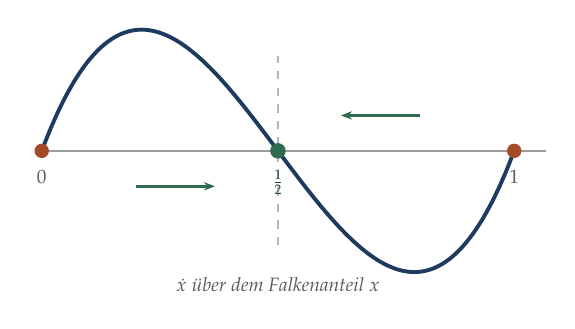
\begin{tikzpicture}[scale=1.0]
\draw[grau!60, line width=0.7pt] (0,0) -- (6.4,0);
\draw[tief, line width=1.4pt, smooth, samples=60, domain=0:6]
  plot ({\x}, {16*(\x/6)*(1-\x/6)*(1-2*\x/6)});
\draw[grau!45, line width=0.5pt, dashed] (3,-1.2) -- (3,1.2);
\fill[akzent] (0,0) circle (2.6pt);
\fill[gruen] (3,0) circle (2.8pt);
\fill[akzent] (6,0) circle (2.6pt);
\draw[gruen, line width=1.0pt, -{Stealth[length=4pt]}] (1.2,-0.45) -- (2.2,-0.45);
\draw[gruen, line width=1.0pt, -{Stealth[length=4pt]}] (4.8,0.45) -- (3.8,0.45);
\node[font=\scriptsize, color=grau, anchor=north] at (0,-0.12) {$0$};
\node[font=\scriptsize, color=gruen!70!black, anchor=north] at (3,-0.12) {$\tfrac12$};
\node[font=\scriptsize, color=grau, anchor=north] at (6,-0.12) {$1$};
\node[font=\scriptsize\itshape, color=grau] at (3.0,-1.7) {$\dot x$ über dem Falkenanteil $x$};
\end{tikzpicture}
\end{center}

\schritt{Eine Bahn}
\begin{center}
{\small
\renewcommand{\arraystretch}{1.48}
\begin{tabular}{@{}P{1.6cm}P{2.2cm}P{2.6cm}@{}}
\toprule
$t$ & $x(t)$ & \\
\midrule
$0$ & $0{,}9000$ & Falken überwiegen\\
$4$ & $0{,}5832$ & \\
$8$ & $0{,}5085$ & \\
$12$ & $0{,}5009$ & \\
$20$ & $0{,}5000$ & \\
\bottomrule
\end{tabular}}
\end{center}

\begin{center}
\begin{minipage}{0.9\textwidth}
\textbf{Die Bevölkerung findet das Gleichgewicht, ohne dass jemand es kennt.}
\end{minipage}
\end{center}
\end{merksatz}

\begin{merksatz}
\boxtitel{Satz 10.2 --- der Zusammenhang}
\begin{center}
{\small
\renewcommand{\arraystretch}{1.52}
\begin{tabular}{@{}P{3.0cm}P{5.6cm}@{}}
\toprule
\textbf{Nash} & Jedes Nash-Gleichgewicht ist eine Ruhelage.\\
\textbf{Stabil $\Rightarrow$ anziehend} & Jede evolutionär stabile Strategie ist eine asymptotisch stabile Ruhelage.\\
\textbf{Nicht umgekehrt} & Es gibt anziehende Ruhelagen, die nicht evolutionär stabil sind --- und Ruhelagen, die kein Nash-Gleichgewicht sind.\\
\bottomrule
\end{tabular}}
\end{center}

\schritt{Zur ersten Zeile}
Im Gleichgewicht haben alle benutzten Strategien dieselbe Eignung (Satz 3.3), also $f_i = \bar f$ und damit $\dot x_i = 0$.

\schritt{Zur dritten Zeile}
Die Ränder $x=0$ und $x=1$ sind stets Ruhelagen --- unabhängig davon, ob sie ein Gleichgewicht sind.

\begin{center}
\begin{minipage}{0.88\textwidth}
\kursiv{Im Leitfall ist $x=1$ eine Ruhelage, obwohl eine reine Falkenbevölkerung von Tauben unterwandert würde. \textbf{Die Gleichung kann den Zustand nicht verlassen, weil keine Tauben vorhanden sind}, die wachsen könnten. Erst die Ableitung $g'(1) = 1 > 0$ zeigt, dass jede noch so kleine Beimischung ausreicht.}
\end{minipage}
\end{center}
\end{merksatz}

\section{Wenn die Bewegung nicht zur Ruhe kommt}

\begin{merksatz}
\boxtitel{Das zyklische Spiel}
Aus Aufgabe 3.1:
\[ A = \begin{pmatrix} 0 & 2 & -1\\ -2 & 0 & 1\\ 1 & -1 & 0 \end{pmatrix}, \qquad \vek p = \left(\tfrac14,\ \tfrac14,\ \tfrac12\right) \]

\schritt{Satz 10.3 --- die Bahnen sind geschlossen}
Für antisymmetrisches $A$ mit innerem Gleichgewicht $\vek p$ ist
\[ H(\vek x) = \sum_i p_i\,\ln x_i \]
entlang jeder Bahn konstant.

\schritt{Beweis}
\kursiv{Erstens:} Antisymmetrie liefert $\vek x^{\!\top} A\vek x = 0$, denn jeder Summand $x_i a_{ij} x_j$ hebt sich gegen $x_j a_{ji} x_i$ auf. Also $\bar f = 0$ und
\[ \dot x_i = x_i\,(A\vek x)_i . \]

\kursiv{Zweitens:}
\[ \frac{\dd H}{\dd t} = \sum_i p_i\,\frac{\dot x_i}{x_i} = \sum_i p_i\,(A\vek x)_i = \vek p^{\!\top} A\,\vek x . \]

\kursiv{Drittens:} Da $\vek p$ ein Gleichgewicht ist, gilt $A\vek p = \vek 0$. Mit $A^{\!\top} = -A$:
\[ \vek p^{\!\top} A\,\vek x = (A^{\!\top}\vek p)^{\!\top}\vek x = (-A\vek p)^{\!\top}\vek x = \vek 0^{\!\top}\vek x = 0 \]
$\blacksquare$

\begin{center}
\begin{minipage}{0.9\textwidth}
\textbf{Die Bahnen laufen auf Niveauflächen von $H$ --- sie kreisen um das Gleichgewicht, ohne es je zu erreichen.}
\end{minipage}
\end{center}

\schritt{Eine Bahn, gerechnet}
Start bei $(0{,}30;\ 0{,}30;\ 0{,}40)$, also $H = -1{,}06013$:
\begin{center}
{\small
\renewcommand{\arraystretch}{1.48}
\begin{tabular}{@{}P{1.4cm}P{3.4cm}P{2.4cm}@{}}
\toprule
$t$ & $\vek x(t)$ & $H$\\
\midrule
$0$ & $(0{,}300;\,0{,}300;\,0{,}400)$ & $-1{,}06013$\\
$40$ & $(0{,}228;\,0{,}181;\,0{,}592)$ & $-1{,}06013$\\
$80$ & $(0{,}224;\,0{,}343;\,0{,}433)$ & $-1{,}06013$\\
$120$ & $(0{,}297;\,0{,}172;\,0{,}531)$ & $-1{,}06013$\\
$200$ & $(0{,}342;\,0{,}208;\,0{,}450)$ & $-1{,}06013$\\
\bottomrule
\end{tabular}}
\end{center}

\kursiv{Die Umlaufdauer beträgt hier etwa $117$ Zeiteinheiten.}

\begin{center}
\begin{minipage}{0.88\textwidth}
\kursiv{Kapitel~9 hatte bereits festgestellt, dass dieses Spiel keine evolutionär stabile Strategie besitzt. \textbf{Hier sieht man, was stattdessen geschieht}: Die Anteile schwanken dauerhaft mit fester Amplitude, die vom Startwert abhängt. Bei einer kalifornischen Eidechsenart mit drei Paarungsstrategien wurde ein solcher Zyklus über zwei Jahrzehnte dokumentiert, mit einer Periode von etwa sechs Jahren.}
\end{minipage}
\end{center}

\schritt{Der Vorbehalt}
\begin{center}
\begin{minipage}{0.88\textwidth}
\kursiv{Die Erhaltungsgröße macht das System zu einem Grenzfall: \textbf{Die kleinste Störung des Modells zerstört sie}, und dann spiralt die Bahn entweder nach innen oder nach außen. Bei Auswärtsspirale läuft die Bevölkerung gegen den Rand, und ein Typ stirbt aus --- woraufhin der Zyklus endet. Welcher Fall eintritt, hängt an Termen, die das Modell gar nicht enthält.}
\end{minipage}
\end{center}
\end{merksatz}

\section{Der Leitfall: Resistenz}

\begin{merksatz}
\boxtitel{Die offene Rechnung aus Band 18}
Dort war die Ausgangslage: Ein Tumor von $10^{12}$ Zellen, eine Mutationsrate von $\mu = 10^{-6}$, also ein resistenter Anteil von
\[ x_0 = 10^{-6} . \]

\begin{center}
{\small
\renewcommand{\arraystretch}{1.5}
\begin{tabular}{@{}P{2.4cm}P{2.6cm}P{2.6cm}@{}}
\toprule
\textbf{Lage} & \textbf{empfindlich} & \textbf{resistent}\\
\midrule
unter Therapie & stark geschädigt & wächst\\
ohne Therapie & wächst gut & zahlt Preis\\
\bottomrule
\end{tabular}}
\end{center}

\kursiv{Als Eignungsdifferenzen:}
\[ r_{\text{an}} = f_R - f_S = +0{,}04 \ \text{je Tag}, \qquad r_{\text{aus}} = -0{,}01 \ \text{je Tag} \]

\schritt{Die Gleichung}
\[ \dot x = x\,(1-x)\,r \]
--- die logistische Gleichung aus Band 18, Kapitel~2, mit der Lösung
\[ x(t) = \frac{x_0\,e^{rt}}{1-x_0+x_0 e^{rt}} . \]

\begin{center}
\begin{minipage}{0.88\textwidth}
\kursiv{Es ist dieselbe Gleichung --- und das ist kein Zufall. \textbf{Die Replikatorgleichung für zwei Typen mit konstanter Eignungsdifferenz \kursiv{ist} die logistische Gleichung.} Was dort als Wachstum unter Ressourcenbegrenzung erschien, ist hier die Verdrängung eines Typs durch einen anderen.}
\end{minipage}
\end{center}
\end{merksatz}

\begin{merksatz}
\boxtitel{Dauertherapie}
Bis zur Hälfte resistenter Zellen:
\[ x(t) = \tfrac12 \quad\Longleftrightarrow\quad e^{rt} = \frac{1-x_0}{x_0} \approx 10^{6} \]
\[ t = \frac{\ln 10^{6}}{0{,}04} = \frac{13{,}82}{0{,}04} = 345 \ \text{Tage} \]

\begin{center}
\begin{minipage}{0.9\textwidth}
\textbf{Nach etwa elf Monaten besteht der Tumor zur Hälfte aus resistenten Zellen.}
\end{minipage}
\end{center}

\begin{center}
\begin{minipage}{0.88\textwidth}
\kursiv{Die Zahl liegt in der Größenordnung klinisch beobachteter Rückfallzeiten bei zielgerichteter Therapie. \textbf{Sie folgt aus zwei Angaben} --- Startanteil und Eignungsdifferenz --- und aus nichts sonst.}
\end{minipage}
\end{center}
\end{merksatz}

\begin{merksatz}
\boxtitel{Adaptive Therapie}
Man behandelt in Zyklen: $T_{\text{an}}$ Tage Therapie, $T_{\text{aus}}$ Tage Pause.

\schritt{Die Bedingung}
Über einen Zyklus darf der resistente Anteil nicht wachsen:
\[ r_{\text{an}}\,T_{\text{an}} + r_{\text{aus}}\,T_{\text{aus}} \ \le\ 0 \]
\[ 0{,}04\,T_{\text{an}} \ \le\ 0{,}01\,T_{\text{aus}} \]

\[ \boxed{\ T_{\text{aus}} \ \ge\ 4\,T_{\text{an}}\ } \]

\begin{center}
\begin{minipage}{0.9\textwidth}
\textbf{Die Pause muss viermal so lang sein wie die Behandlung.}
\end{minipage}
\end{center}

\schritt{Die Zahlen}
\begin{center}
{\small
\renewcommand{\arraystretch}{1.48}
\begin{tabular}{@{}P{2.4cm}P{2.2cm}P{2.8cm}@{}}
\toprule
\textbf{Schema} & \textbf{Dauer} & \textbf{resistenter Anteil}\\
\midrule
$60$ an, $60$ aus & $960$ d & $6{,}4\cdot10^{-1}$\\
$60$ an, $180$ aus & $1920$ d & $1{,}2\cdot10^{-4}$\\
$60$ an, $240$ aus & $2400$ d & $1{,}0\cdot10^{-6}$\\
$60$ an, $300$ aus & $2880$ d & $8{,}2\cdot10^{-9}$\\
\midrule
Dauertherapie & $960$ d & $\approx 1$\\
\bottomrule
\end{tabular}}
\end{center}

\begin{center}
\begin{minipage}{0.9\textwidth}
\textbf{Bei $60$ an und $240$ aus bleibt der resistente Anteil exakt auf dem Ausgangswert --- beliebig lange.}
\end{minipage}
\end{center}

\begin{center}
\begin{minipage}{0.88\textwidth}
\kursiv{Die dritte Zeile ist der Grenzfall: Der Netto-Exponent ist genau null. \textbf{Darüber hinaus schrumpft der resistente Anteil sogar}, wie die vierte Zeile zeigt. Das ist die spieltheoretische Begründung, die Band 18, Kapitel~14 offenließ: Die empfindlichen Zellen sind kein Übel, das man beseitigen sollte, sondern das Mittel, mit dem die resistenten unterdrückt werden.}
\end{minipage}
\end{center}

\schritt{Der Preis}
\begin{center}
{\small
\renewcommand{\arraystretch}{1.5}
\begin{tabular}{@{}P{2.4cm}P{6.2cm}@{}}
\toprule
\textbf{Tumorlast} & Der Tumor bleibt bestehen und wächst in den Pausen. Das Ziel ist Beherrschung, nicht Heilung.\\
\textbf{Nur $20$ Prozent} & Behandelt wird ein Fünftel der Zeit. Wer eine Heilung anstrebt, gibt sie damit auf.\\
\textbf{Messbarkeit} & Man muss die Tumorlast häufig messen, um die Zyklen zu steuern.\\
\bottomrule
\end{tabular}}
\end{center}

\begin{center}
\begin{minipage}{0.88\textwidth}
\kursiv{\textbf{Der Ansatz eignet sich nicht für Lagen, in denen Heilung erreichbar ist.} Er ist für unheilbare, aber beherrschbare Erkrankungen gedacht --- und dort verspricht er Jahre statt Monate. Klinische Prüfungen bei einer Prostatakarzinomform zeigten seit 2017 eine deutliche Verlängerung der Beherrschungsdauer bei geringerer Gesamtdosis; die Übertragbarkeit auf andere Tumoren ist Gegenstand laufender Studien.}
\end{minipage}
\end{center}
\end{merksatz}

\section{Der Bruchfall}

\begin{warnung}
\boxtitelr{Was die Gleichung nicht enthält}
\begin{center}
{\small
\renewcommand{\arraystretch}{1.52}
\begin{tabular}{@{}P{2.4cm}P{6.2cm}@{}}
\toprule
\textbf{Keine Mutation} & Ausgestorbene Typen kehren nicht zurück. In der Biologie tun sie es.\\
\textbf{Kein Zufall} & Endliche Bevölkerungen schwanken; die Gleichung beschreibt den Mittelwert.\\
\textbf{Kein Raum} & Jeder trifft jeden. Räumliche Modelle liefern andere Ergebnisse.\\
\textbf{Feste Auszahlungen} & Die Matrix ändert sich nicht --- im Leitfall eine grobe Vereinfachung.\\
\bottomrule
\end{tabular}}
\end{center}

\schritt{Zur ersten Zeile}
Fügt man einen Mutationsterm hinzu, so verschwinden die Randruhelagen.

\begin{center}
\begin{minipage}{0.88\textwidth}
\kursiv{Die entstehende Gleichung heißt Replikator-Mutator-Gleichung; sie hat innere Ruhelagen nahe den alten Rändern. \textbf{Für den Leitfall ist das wesentlich}: Ein resistenter Anteil von null ist biologisch unerreichbar, weil ständig neue Mutationen entstehen --- genau das war Band 18, Kapitel~14 mit $N_c = 1/\mu$.}
\end{minipage}
\end{center}

\schritt{Zur vierten Zeile}
\begin{center}
\begin{minipage}{0.88\textwidth}
\kursiv{Die Eignungsdifferenzen $+0{,}04$ und $-0{,}01$ wurden als konstant angenommen. Tatsächlich hängen sie von der Tumorgröße, der Durchblutung, dem Sauerstoffangebot und der Dosis ab. \textbf{Die Rechnung liefert daher eine Größenordnung und ein Verhältnis} --- die Pause muss ein Vielfaches der Therapie betragen --- aber keine Therapieplanung. Wer sie so benutzt, begeht den Fehler der ersten Warnung des Vorworts.}
\end{minipage}
\end{center}
\end{warnung}

\section{Übungsaufgaben}

\begin{aufgabe}
\boxtitel{Aufgabe 10.1 --- Ein Koordinationsspiel}
Bestimmen Sie die Replikatordynamik der Hirschjagd aus Kapitel~5 und analysieren Sie die Ruhelagen.
\[ A = \begin{pmatrix} 4 & 0\\ 3 & 3 \end{pmatrix} \]

\loesung
\schritt{Schritt 1 --- Die Eignungen}
Mit $x$ als Anteil derer, die gemeinsam vorgehen:
\[ f_G = 4x + 0\,(1-x) = 4x \]
\[ f_A = 3x + 3\,(1-x) = 3 \]

\schritt{Schritt 2 --- Die Gleichung}
\[ \dot x = x\,(1-x)\,(4x-3) \]

\schritt{Schritt 3 --- Die Ruhelagen}
\[ x = 0, \qquad x = \tfrac34, \qquad x = 1 \]

\schritt{Schritt 4 --- Die Stabilität}
\begin{center}
{\small
\renewcommand{\arraystretch}{1.5}
\begin{tabular}{@{}P{1.4cm}P{3.4cm}P{2.2cm}@{}}
\toprule
$x$ & \textbf{Verhalten nahebei} & \\
\midrule
$0$ & $\dot x \approx -3x < 0$ & \textcolor{gruen}{anziehend}\\
$\tfrac34$ & Vorzeichen\-wechsel $-$ nach $+$ & \textcolor{akzent}{abstoßend}\\
$1$ & $\dot x \approx (1-x) > 0$ & \textcolor{gruen}{anziehend}\\
\bottomrule
\end{tabular}}
\end{center}

\kursiv{Zur mittleren Zeile:} Für $x < \tfrac34$ ist $4x-3 < 0$, also $\dot x < 0$; für $x > \tfrac34$ ist $\dot x > 0$.

\schritt{Schritt 5 --- Der Einzugsbereich}
\begin{center}
\begin{minipage}{0.9\textwidth}
\textbf{Startet die Bevölkerung mit weniger als $75$ Prozent Kooperierenden, so stirbt die Zusammenarbeit aus.} Darüber setzt sie sich vollständig durch.
\end{minipage}
\end{center}

\begin{center}
\begin{minipage}{0.88\textwidth}
\kursiv{Die Schwelle $\tfrac34$ ist genau die Vertrauensschwelle $q^{*} = T/R$ aus Aufgabe 5.3. \textbf{Was dort eine Erwartung war, ist hier ein Anfangszustand} --- und das ist der begriffliche Gewinn dieses Kapitels: Die Frage \enquote{traut man dem anderen zu, mitzuziehen?} wird zur Frage \enquote{wie viele ziehen bereits mit?}.}
\end{minipage}
\end{center}

\schritt{Schritt 6 --- Die Folge für die Praxis}
\begin{center}
\begin{minipage}{0.88\textwidth}
\kursiv{Eine Hirschjagd löst man nicht durch Überzeugungsarbeit im Einzelfall, sondern indem man die Bevölkerung über die Schwelle hebt --- etwa durch eine anfängliche Förderung, die nach Erreichen der Schwelle entfallen kann. \textbf{Die Maßnahme muss nur einmal wirken, nicht dauerhaft}, und das unterscheidet sie von der Anreizänderung im Gefangenendilemma, die bestehen bleiben muss.}
\end{minipage}
\end{center}
\end{aufgabe}

\begin{aufgabe}
\boxtitel{Aufgabe 10.2 --- Die Erhaltungsgröße prüfen}
Weisen Sie für das zyklische Spiel nach, dass $H$ konstant ist, und bestimmen Sie $H$ für zwei Punkte derselben Bahn.

\loesung
\schritt{Schritt 1 --- Die Voraussetzungen prüfen}
\kursiv{Antisymmetrie:} $a_{12} = 2 = -a_{21}$, $a_{13} = -1 = -a_{31}$, $a_{23} = 1 = -a_{32}$ \checkmark

\kursiv{Gleichgewicht:} $A\vek p$ mit $\vek p = (\tfrac14,\tfrac14,\tfrac12)$:
\begin{align*}
(A\vek p)_1 &= 0\cdot\tfrac14 + 2\cdot\tfrac14 - 1\cdot\tfrac12 = \tfrac12-\tfrac12 = 0\\
(A\vek p)_2 &= -2\cdot\tfrac14 + 0 + 1\cdot\tfrac12 = -\tfrac12+\tfrac12 = 0\\
(A\vek p)_3 &= 1\cdot\tfrac14 - 1\cdot\tfrac14 + 0 = 0
\end{align*}
\checkmark

\schritt{Schritt 2 --- $H$ am Startpunkt}
\[ H = \tfrac14\ln 0{,}300 + \tfrac14\ln 0{,}300 + \tfrac12\ln 0{,}400 \]
\[ = \tfrac14(-1{,}20397) + \tfrac14(-1{,}20397) + \tfrac12(-0{,}91629) \]
\[ = -0{,}30099 - 0{,}30099 - 0{,}45814 = \mathbf{-1{,}06013} \]

\schritt{Schritt 3 --- $H$ an einem späteren Punkt}
Bei $\vek x = (0{,}2280;\ 0{,}1805;\ 0{,}5915)$:
\[ H = \tfrac14(-1{,}47841) + \tfrac14(-1{,}71202) + \tfrac12(-0{,}52509) \]
\[ = -0{,}36960 - 0{,}42801 - 0{,}26255 = \mathbf{-1{,}06016} \]

\begin{center}
\begin{minipage}{0.9\textwidth}
\textbf{Übereinstimmung bis auf Rundung --- die Größe bleibt erhalten.}
\end{minipage}
\end{center}

\schritt{Schritt 4 --- Der Wert am Gleichgewicht}
\[ H(\vek p) = \tfrac14\ln\tfrac14 + \tfrac14\ln\tfrac14 + \tfrac12\ln\tfrac12 \]
\[ = \tfrac12(-1{,}38629) + \tfrac12(-0{,}69315) = -0{,}69315-0{,}34657 = -1{,}03972 \]

\begin{center}
\begin{minipage}{0.9\textwidth}
\textbf{Das Gleichgewicht hat den größten Wert von $H$} --- alle Bahnen liegen darunter.
\end{minipage}
\end{center}

\schritt{Schritt 5 --- Warum das ein Maximum ist}
Die Funktion $\sum p_i \ln x_i$ wird unter der Nebenbedingung $\sum x_i = 1$ bei $x_i = p_i$ maximal.

\kursiv{Grund:} Die Differenz ist
\[ H(\vek p) - H(\vek x) = \sum_i p_i\ln\frac{p_i}{x_i} = D(\vek p\,\|\,\vek x) \ \ge\ 0 \]
--- die relative Entropie aus Band 20, Satz 4.4.

\begin{center}
\begin{minipage}{0.88\textwidth}
\kursiv{\textbf{Die Erhaltungsgröße dieses Kapitels ist bis auf ein Vorzeichen die Kullback-Leibler-Divergenz.} Die Bahnen laufen auf Flächen konstanten Abstands zum Gleichgewicht, gemessen in dieser Größe. Dass ausgerechnet das Werkzeug aus Band 20, Teil~II hier wieder auftaucht, ist eine der unerwarteteren Verbindungen zwischen den Bänden.}
\end{minipage}
\end{center}

\schritt{Schritt 6 --- Die Folge}
\begin{center}
\begin{minipage}{0.88\textwidth}
\kursiv{Da $D$ längs der Bahn konstant bleibt, nähert sich die Bevölkerung dem Gleichgewicht nie an --- und entfernt sich auch nie weiter. \textbf{Das Gleichgewicht ist stabil im Sinne von Ljapunow, aber nicht anziehend.} In der Sprache von Kapitel~9: Es ist ein Nash-Gleichgewicht, aber keine evolutionär stabile Strategie, und beides hat dieselbe Ursache.}
\end{minipage}
\end{center}
\end{aufgabe}

\begin{aufgabe}
\boxtitel{Aufgabe 10.3 --- Das Therapieschema auslegen}
Bei einem anderen Tumor gelten $r_{\text{an}} = 0{,}06$ und $r_{\text{aus}} = -0{,}03$ je Tag, Startanteil $x_0 = 10^{-5}$. Legen Sie ein Schema aus und vergleichen Sie mit der Dauertherapie.

\loesung
\schritt{Schritt 1 --- Die Dauertherapie}
\[ t = \frac{\ln\bigl((1-x_0)/x_0\bigr)}{r_{\text{an}}} = \frac{\ln 10^{5}}{0{,}06} = \frac{11{,}513}{0{,}06} = 192 \ \text{Tage} \]

\begin{center}
\begin{minipage}{0.9\textwidth}
\textbf{Nach gut sechs Monaten ist die Hälfte der Zellen resistent.}
\end{minipage}
\end{center}

\schritt{Schritt 2 --- Die Bedingung für das Gleichgewicht}
\[ 0{,}06\,T_{\text{an}} \ \le\ 0{,}03\,T_{\text{aus}} \quad\Longrightarrow\quad T_{\text{aus}} \ \ge\ 2\,T_{\text{an}} \]

\begin{center}
\begin{minipage}{0.9\textwidth}
\textbf{Hier genügt die doppelte Pause statt der vierfachen.}
\end{minipage}
\end{center}

\schritt{Schritt 3 --- Der Grund}
\begin{center}
{\small
\renewcommand{\arraystretch}{1.5}
\begin{tabular}{@{}P{2.4cm}P{2.0cm}P{2.0cm}P{2.0cm}@{}}
\toprule
& $r_{\text{an}}$ & $|r_{\text{aus}}|$ & \textbf{Verhältnis}\\
\midrule
Leitfall & $0{,}04$ & $0{,}01$ & $4$\\
hier & $0{,}06$ & $0{,}03$ & $2$\\
\bottomrule
\end{tabular}}
\end{center}

\begin{center}
\begin{minipage}{0.88\textwidth}
\kursiv{\textbf{Nicht die absolute Größe der Raten entscheidet, sondern ihr Verhältnis.} Die Therapie wirkt hier zwar stärker ($0{,}06$ statt $0{,}04$), aber der Eignungspreis der Resistenz ist ebenfalls höher ($0{,}03$ statt $0{,}01$) --- und das zweite überwiegt. Ein hoher Resistenzpreis ist das günstigste Merkmal für die adaptive Therapie.}
\end{minipage}
\end{center}

\schritt{Schritt 4 --- Ein konkretes Schema}
Mit $T_{\text{an}} = 30$ und $T_{\text{aus}} = 90$ Tagen:
\[ 0{,}06\cdot30 + (-0{,}03)\cdot90 = 1{,}8 - 2{,}7 = -0{,}9 \ \text{je Zyklus} \]

\begin{center}
\begin{minipage}{0.9\textwidth}
\textbf{Der resistente Anteil schrumpft um den Faktor $e^{-0{,}9} = 0{,}407$ je Zyklus.}
\end{minipage}
\end{center}

\kursiv{Nach zehn Zyklen, also $1200$ Tagen:}
\[ x \approx 10^{-5}\cdot e^{-9} = 10^{-5}\cdot1{,}23\cdot10^{-4} = 1{,}2\cdot10^{-9} \]

\schritt{Schritt 5 --- Der Vorbehalt}
\begin{center}
\begin{minipage}{0.88\textwidth}
\kursiv{Die Näherung $x \approx x_0 e^{\sum r t}$ gilt nur, solange $x \ll 1$ --- dann ist der Faktor $(1-x)$ in der Replikatorgleichung nahe eins. \textbf{Bei größeren Anteilen muss man die vollständige logistische Lösung verwenden}, und dann verlangsamt sich sowohl das Wachstum als auch die Schrumpfung. Für die hier auftretenden Größenordnungen ist die Näherung unbedenklich.}
\end{minipage}
\end{center}

\schritt{Schritt 6 --- Und der Behandlungsanteil}
\begin{center}
\renewcommand{\arraystretch}{1.48}
\begin{tabular}{@{}P{2.2cm}P{2.8cm}P{2.2cm}@{}}
\toprule
\textbf{Fall} & \textbf{Therapie\-anteil} & \\
\midrule
Leitfall & $20\,\%$ & $60/300$\\
hier & $25\,\%$ & $30/120$\\
\bottomrule
\end{tabular}
\end{center}

\begin{center}
\begin{minipage}{0.88\textwidth}
\kursiv{In beiden Fällen wird ein knappes Viertel der Zeit behandelt --- und die Beherrschungsdauer steigt von Monaten auf Jahre. \textbf{Weniger Medikament wirkt länger}, und das ist der Satz, der bei dieser Therapieform am meisten Widerstand hervorruft.}
\end{minipage}
\end{center}
\end{aufgabe}

\begin{geschichte}
\boxtitelg{Eine Gleichung aus der Ökologie}
\Person{Peter Taylor} und \Person{Leo Jonker} führten die Replikatorgleichung 1978 ein, um Maynard Smiths statischen Begriff dynamisch zu fassen.

\begin{center}
\begin{minipage}{0.9\textwidth}
\kursiv{Sie zeigten, dass jede evolutionär stabile Strategie eine asymptotisch stabile Ruhelage ist --- und dass die Umkehrung nicht gilt. \textbf{Damit war klar, dass die beiden Begriffe nicht dasselbe sind}, obwohl sie oft gleichgesetzt werden.}
\end{minipage}
\end{center}

\schritt{Der Name}
Er stammt von \Person{Peter Schuster} und \Person{Karl Sigmund} (1983), die den Zusammenhang zu den Gleichungen der Chemie herstellten.

\begin{center}
\begin{minipage}{0.9\textwidth}
\kursiv{Dieselbe Gleichung beschreibt die Konkurrenz sich selbst vervielfältigender Moleküle --- Eigens Hyperzyklen zur Entstehung des Lebens --- und die Konkurrenz von Verhaltensweisen in einer Tierpopulation. \textbf{Sie ist überdies gleichwertig zu den Lotka-Volterra-Gleichungen aus Band 18, Kapitel~4}, mit einer Variablen weniger.}
\end{minipage}
\end{center}

\schritt{Die Eidechsen}
\Person{Barry Sinervo} und \Person{Curt Lively} berichteten 1996 über eine kalifornische Eidechse mit drei erblichen Paarungsstrategien, kenntlich an der Kehlfarbe.

\begin{center}
\begin{minipage}{0.9\textwidth}
\kursiv{Orange schlägt Blau, Blau schlägt Gelb, Gelb schlägt Orange --- ein zyklisches Spiel in der Natur, mit einer beobachteten Periode von etwa sechs Jahren. \textbf{Die Arbeit gilt als der überzeugendste Feldnachweis für Satz 10.3}, obwohl spätere Untersuchungen zeigten, dass der Zyklus weniger regelmäßig verläuft als zunächst berichtet.}
\end{minipage}
\end{center}

\schritt{Gatenby}
\Person{Robert Gatenby} schlug die adaptive Therapie ab 2009 vor, ausdrücklich unter Berufung auf die evolutionäre Spieltheorie --- und auf die Schädlingsbekämpfung.

\begin{center}
\begin{minipage}{0.9\textwidth}
\kursiv{Dort war seit Jahrzehnten bekannt, dass die vollständige Ausrottung eines Schädlings die Resistenzentwicklung beschleunigt, während eine Restpopulation empfindlicher Tiere sie bremst. \textbf{Die Übertragung auf die Onkologie stieß auf erheblichen Widerstand}, weil sie der Regel widerspricht, die größtmögliche verträgliche Dosis zu geben. Die erste klinische Prüfung begann 2015.}
\end{minipage}
\end{center}
\end{geschichte}

\begin{forschung}
\boxtitelp{Dynamik heute}
\begin{center}
{\small
\renewcommand{\arraystretch}{1.45}
\begin{tabular}{@{}P{2.8cm}P{5.4cm}@{}}
\toprule
\textbf{Andere Dynamiken} & Nachahmen, bestes Antworten, Verstärkungslernen --- jede mit eigenem Langzeitverhalten.\\
\textbf{Chaos} & Ab drei Strategien und geeigneten Auszahlungen tritt Chaos auf.\\
\textbf{Steuerung} & Wie man eine Bevölkerung gezielt in ein gewünschtes Gleichgewicht lenkt.\\
\bottomrule
\end{tabular}}
\end{center}

\schritt{Zur zweiten Zeile}
Bei vier Strategien wurden chaotische Bahnen nachgewiesen.

\begin{center}
\begin{minipage}{0.88\textwidth}
\kursiv{Es ist dasselbe Phänomen wie in Band 18, Kapitel~3: eine einfache Gleichung mit unvorhersehbarem Langzeitverhalten. \textbf{Eine Bevölkerung kann also dauerhaft unregelmäßig schwanken, ohne dass sich etwas an den Regeln ändert} --- und wer aus solchen Daten auf veränderte Umstände schließt, irrt.}
\end{minipage}
\end{center}

\schritt{Zur dritten Zeile}
Die adaptive Therapie ist ein Beispiel: Man verändert die Auszahlungen zeitweise, um die Bahn zu lenken.

\begin{center}
\begin{minipage}{0.88\textwidth}
\kursiv{Verwandte Ansätze arbeiten mit zwei abwechselnden Wirkstoffen, deren Resistenzen einander ausschließen --- man nennt das \Begriff{kollaterale Empfindlichkeit}. \textbf{Damit wird aus dem Spiel gegen einen Gegner ein Spiel gegen zwei}, und der Tumor kann nicht beiden zugleich ausweichen. Die Auswahl geeigneter Wirkstoffpaare ist ein aktives Forschungsfeld.}
\end{minipage}
\end{center}
\end{forschung}

\begin{merksatz}
\boxtitel{Was Sie jetzt können}
\begin{center}
\renewcommand{\arraystretch}{1.5}
\begin{tabular}{@{}P{3.0cm}P{5.6cm}@{}}
\toprule
\textbf{Definition 10.1} & wächst, wer überdurchschnittlich ist\\
\textbf{Zwei Typen} & $\dot x = x(1-x)(f_1-f_2)$\\
\textbf{Satz 10.2} & stabil $\Rightarrow$ anziehend, nicht umgekehrt\\
\textbf{Satz 10.3} & antisymmetrisch: geschlossene Bahnen\\
\textbf{Adaptive Therapie} & $T_{\text{aus}} \ge \frac{r_{\text{an}}}{|r_{\text{aus}}|}\,T_{\text{an}}$\\
\bottomrule
\end{tabular}
\end{center}

\begin{center}
\begin{minipage}{0.88\textwidth}
\kursiv{Damit endet Teil~IV. Bisher waren die Regeln gegeben. Ab Kapitel~11 fragen wir, wie man sie entwirft --- und stoßen auf eine Grenze, die kein Entwurf überwindet.}
\end{minipage}
\end{center}
\end{merksatz}

\part{Regeln entwerfen}

\chapter{Kollektivgüter und soziale Dilemmata}

\section{Von zwei auf viele}

\begin{merksatz}
\boxtitel{Der Leitfall: ein gemeinsamer Nachtdienstpool}
Vier Abteilungen des Klinikums können Personal in einen gemeinsamen Bereitschaftspool geben. Der Pool arbeitet wirksamer als getrennte Dienste --- jede eingebrachte Stunde erbringt das Doppelte, verteilt auf alle vier.

\begin{center}
{\small
\renewcommand{\arraystretch}{1.5}
\begin{tabular}{@{}P{2.6cm}P{2.0cm}P{2.8cm}@{}}
\toprule
\textbf{Größe} & \textbf{Wert} & \\
\midrule
Abteilungen $n$ & $4$ & \\
Verfügbar $e$ & $10$ Stunden & je Abteilung\\
Verstärkung $r$ & $2$ & Wirksamkeits\-gewinn\\
\bottomrule
\end{tabular}}
\end{center}

\schritt{Die Auszahlung}
Gibt Abteilung $i$ den Beitrag $c_i$ ab, so erhält sie
\[ \Aus_i = \underbrace{e-c_i}_{\text{behalten}} \;+\; \underbrace{\frac{r}{n}\sum_j c_j}_{\text{Anteil am Pool}} . \]
\end{merksatz}

\begin{merksatz}
\boxtitel{Satz 11.1 --- das Dilemma}
Für $1 < r < n$ gilt:
\begin{center}
{\small
\renewcommand{\arraystretch}{1.5}
\begin{tabular}{@{}P{2.4cm}P{6.2cm}@{}}
\toprule
\textbf{Gleichgewicht} & Niemand gibt etwas: $c_i = 0$ ist strikt dominant.\\
\textbf{Optimum} & Alle geben alles: $c_i = e$ maximiert die Summe.\\
\bottomrule
\end{tabular}}
\end{center}

\schritt{Beweis --- das Gleichgewicht}
Der Grenzertrag einer zusätzlich eingebrachten Einheit beträgt für den Einbringenden
\[ \frac{\partial \Aus_i}{\partial c_i} = -1 + \frac{r}{n} . \]

Für $r < n$ ist das negativ. Jede Einheit, die man abgibt, kostet unter dem Strich.

\kursiv{Im Leitfall:} $-1+\tfrac24 = -\tfrac12$.

\begin{center}
\begin{minipage}{0.9\textwidth}
\textbf{Jede eingebrachte Stunde kostet die Abteilung eine halbe Stunde --- unabhängig davon, was die anderen tun.}
\end{minipage}
\end{center}

\schritt{Beweis --- das Optimum}
Der Gesamtertrag beträgt
\[ \sum_i \Aus_i = n\,e - \sum_j c_j + r\sum_j c_j = n\,e + (r-1)\sum_j c_j . \]

Für $r > 1$ wächst er mit jedem Beitrag. $\blacksquare$

\schritt{Die Zahlen}
\begin{center}
{\small
\renewcommand{\arraystretch}{1.5}
\begin{tabular}{@{}P{2.8cm}P{2.0cm}P{2.6cm}@{}}
\toprule
\textbf{Lage} & \textbf{je Abt.} & \textbf{gesamt}\\
\midrule
alle geben $10$ & $20$ & $80$\\
alle geben $0$ & $10$ & $40$\\
\midrule
einer gibt $10$ & $5$ & \\
die drei anderen & $15$ & $50$\\
\bottomrule
\end{tabular}}
\end{center}

\begin{center}
\begin{minipage}{0.9\textwidth}
\textbf{Das Gleichgewicht verschenkt die Hälfte.} Und wer allein beiträgt, steht schlechter da als ohne den Pool.
\end{minipage}
\end{center}

\begin{center}
\begin{minipage}{0.88\textwidth}
\kursiv{Die letzte Zeile ist die eigentliche Schwierigkeit: \textbf{Der einzelne Beitragende wird bestraft, während die anderen gewinnen.} Bei $n=2$ ist das genau das Gefangenendilemma aus Kapitel~5, mit $T=15$, $R=20$ --- nein, hier liegt ein Unterschied: Der Beitrag ist teilbar, und das erlaubt Zwischenstufen.}
\end{minipage}
\end{center}
\end{merksatz}

\begin{warnung}
\boxtitelr{Die Schwelle liegt bei $r = n$}
\begin{center}
{\small
\renewcommand{\arraystretch}{1.48}
\begin{tabular}{@{}P{1.6cm}P{2.2cm}P{3.2cm}@{}}
\toprule
$r$ & \textbf{Grenzertrag} & \\
\midrule
$1$ & $-\tfrac34$ & kein Gewinn zu verteilen\\
$2$ & $-\tfrac12$ & \textcolor{akzent}{Dilemma}\\
$3$ & $-\tfrac14$ & \textcolor{akzent}{Dilemma}\\
$4$ & $0$ & Gleichstand\\
$5$ & $+\tfrac14$ & \textcolor{gruen}{Beitrag dominant}\\
\bottomrule
\end{tabular}}
\end{center}

\begin{center}
\begin{minipage}{0.9\textwidth}
\textbf{Erst wenn der Gewinn die Gruppengröße übersteigt, löst sich das Dilemma von selbst.}
\end{minipage}
\end{center}

\begin{center}
\begin{minipage}{0.88\textwidth}
\kursiv{Daraus folgt unmittelbar, warum große Gruppen das Problem verschärfen: \textbf{Mit wachsendem $n$ muss $r$ mitwachsen}, sonst wird der Grenzertrag immer negativer. Bei $n=100$ bräuchte man eine hundertfache Verstärkung --- und die gibt es nicht. Das ist der Grund, warum Zusammenarbeit in kleinen Gruppen leichter gelingt, und er hat nichts mit Vertrautheit zu tun.}
\end{minipage}
\end{center}
\end{warnung}

\section{Die Allmendetragik}

\begin{merksatz}
\boxtitel{Der zweite Grundtyp}
Beim Kollektivgut geht es um das Einbringen, bei der Allmende um das Entnehmen.

\begin{center}
{\small
\renewcommand{\arraystretch}{1.5}
\begin{tabular}{@{}P{2.4cm}P{6.2cm}@{}}
\toprule
\textbf{Kollektivgut} & Niemand kann ausgeschlossen werden; wer beiträgt, trägt die Kosten allein.\\
\textbf{Allmende} & Niemand kann ausgeschlossen werden; wer entnimmt, mindert den Bestand für alle.\\
\bottomrule
\end{tabular}}
\end{center}

\schritt{Das Modell}
$n$ Nutzer entnehmen je $x_i$; der Ertrag je Einheit sinkt mit der Gesamtentnahme $X = \sum_i x_i$:
\[ \Aus_i = x_i\,(a - b\,X) - c\,x_i \]

\schritt{Das Gleichgewicht}
\[ \frac{\partial \Aus_i}{\partial x_i} = a - b\,X - b\,x_i - c = 0 \]

\kursiv{Man beachte den mittleren Term:} Der Nutzer berücksichtigt nur die Minderung, die \kursiv{seine eigene} Entnahme bei \kursiv{seinen eigenen} Einheiten verursacht --- nicht die bei den anderen.

Im symmetrischen Fall $x_i = X/n$:
\[ a - b\,X - \frac{b\,X}{n} - c = 0 \quad\Longrightarrow\quad X_{\text{GG}} = \frac{n\,(a-c)}{b\,(n+1)} \]

\schritt{Das Optimum}
\[ \max_X \ X\,(a-bX) - cX \quad\Longrightarrow\quad a - 2bX - c = 0 \quad\Longrightarrow\quad X^{*} = \frac{a-c}{2b} \]

\schritt{Satz 11.2 --- der Übernutzungsfaktor}
\[ \frac{X_{\text{GG}}}{X^{*}} = \frac{2n}{n+1} \]

\begin{center}
{\small
\renewcommand{\arraystretch}{1.48}
\begin{tabular}{@{}P{1.4cm}P{1.8cm}P{2.2cm}P{2.4cm}@{}}
\toprule
$n$ & \textbf{Faktor} & $X_{\text{GG}}$ & \textbf{Ertrag}\\
\midrule
$1$ & $1{,}00$ & $40{,}0$ & $100\,\%$\\
$2$ & $1{,}33$ & $53{,}3$ & $89\,\%$\\
$4$ & $1{,}60$ & $64{,}0$ & $64\,\%$\\
$10$ & $1{,}82$ & $72{,}7$ & $33\,\%$\\
$100$ & $1{,}98$ & $79{,}2$ & $4\,\%$\\
\bottomrule
\end{tabular}}
\end{center}
\kursiv{Mit $a=100$, $b=1$, $c=20$, also $X^{*}=40$.}

\begin{center}
\begin{minipage}{0.9\textwidth}
\textbf{Die Übernutzung nähert sich dem Faktor zwei --- der Ertrag geht gegen null.}
\end{minipage}
\end{center}

\begin{center}
\begin{minipage}{0.88\textwidth}
\kursiv{Bemerkenswert ist das Auseinanderklaffen von Menge und Ertrag: Bei hundert Nutzern wird nur doppelt so viel entnommen, aber der Ertrag fällt auf ein Fünfundzwanzigstel. \textbf{Der Grund ist die Krümmung}: Nahe dem Punkt, an dem der Ertrag null wird ($X = 80$), bringt jede weitere Einheit fast nichts mehr ein und schädigt alle übrigen. Der Einzelne merkt davon nur den eigenen Anteil.}
\end{minipage}
\end{center}

\schritt{Der Sonderfall $n=1$}
\begin{center}
\begin{minipage}{0.9\textwidth}
\textbf{Ein einziger Nutzer wählt das Optimum.} Das Problem entsteht ausschließlich durch die Aufteilung.
\end{minipage}
\end{center}

\begin{center}
\begin{minipage}{0.88\textwidth}
\kursiv{Daraus zog man lange den Schluss, Privateigentum oder staatliche Verwaltung seien die einzigen Auswege. \textbf{Das ist voreilig}, wie Abschnitt 11.4 zeigt.}
\end{minipage}
\end{center}
\end{merksatz}

\section{Was hilft}

\begin{merksatz}
\boxtitel{Bestrafung}
Man erlaubt den Beteiligten, andere auf eigene Kosten zu bestrafen: Wer $k$ aufwendet, fügt dem Bestraften $m$ zu.

\schritt{Wann sie abschreckt}
Der Trittbrettgewinn je nicht eingebrachter Einheit beträgt
\[ 1 - \frac{r}{n} = \tfrac12 \quad\text{im Leitfall.} \]

Eine erwartete Strafe von mehr als $\tfrac12$ je Einheit schreckt ab.

\schritt{Das eigentliche Problem}
\begin{center}
\begin{minipage}{0.9\textwidth}
\textbf{Bestrafen kostet den Bestrafer --- und nützt allen. Es ist selbst ein Kollektivgut.}
\end{minipage}
\end{center}

\begin{center}
\begin{minipage}{0.88\textwidth}
\kursiv{Damit ist das Dilemma eine Ebene höher verschoben, nicht gelöst. \textbf{Man nennt das das Dilemma zweiter Ordnung.} Im rein eigennützigen Modell straft niemand, und die Drohung ist unglaubwürdig --- genau die Lage aus Kapitel~7.}
\end{minipage}
\end{center}

\schritt{Was Versuche zeigen}
\Person{Ernst Fehr} und \Person{Simon Gächter} führten 2000 Versuche mit und ohne Strafmöglichkeit durch.

\begin{center}
{\small
\renewcommand{\arraystretch}{1.5}
\begin{tabular}{@{}P{2.6cm}P{5.8cm}@{}}
\toprule
\textbf{Ohne Strafe} & Die Beiträge beginnen bei etwa der Hälfte und fallen über zehn Runden gegen null.\\
\textbf{Mit Strafe} & Die Beiträge steigen und bleiben nahe dem Maximum.\\
\bottomrule
\end{tabular}}
\end{center}

\begin{center}
\begin{minipage}{0.88\textwidth}
\kursiv{Und zwar auch dann, wenn die Gruppen nach jeder Runde neu zusammengesetzt werden --- also ohne jede Aussicht auf eigenen Nutzen. \textbf{Menschen bestrafen, obwohl es sich nicht lohnt}, und das ist die verlässlichste Abweichung vom eigennützigen Modell, die dieses Fach kennt. Kapitel~15 behandelt, was daraus folgt.}
\end{minipage}
\end{center}

\schritt{Der Vorbehalt}
\begin{center}
\begin{minipage}{0.88\textwidth}
\kursiv{Wird auch das Bestrafen bestraft --- Vergeltung gegen den Bestrafer ---, so bricht der Nutzen zusammen. In Versuchen mit dieser Möglichkeit sinkt der Gesamtertrag unter den ohne jede Strafe. \textbf{Bestrafung wirkt nur, wenn sie ihrerseits gedeckt ist}, und das verlangt eine Instanz oder eine geteilte Norm.}
\end{minipage}
\end{center}
\end{merksatz}

\begin{merksatz}
\boxtitel{Die acht Regeln von Ostrom}
\Person{Elinor Ostrom} untersuchte ab den 1970er Jahren Allmenden, die über Jahrhunderte funktionierten --- Almen, Bewässerungssysteme, Fischgründe.

\begin{center}
{\small
\renewcommand{\arraystretch}{1.48}
\begin{tabular}{@{}P{0.8cm}P{7.6cm}@{}}
\toprule
$1$ & Klare Grenzen: Wer ist berechtigt, und wo?\\
$2$ & Regeln, die zu den örtlichen Verhältnissen passen.\\
$3$ & Die Betroffenen können die Regeln mitgestalten.\\
$4$ & Überwachung durch die Beteiligten selbst.\\
$5$ & Abgestufte Strafen --- kleine Vergehen, kleine Folgen.\\
$6$ & Zugängliche Verfahren zur Streitschlichtung.\\
$7$ & Anerkennung des Selbstverwaltungsrechts von außen.\\
$8$ & Bei großen Systemen: mehrere Ebenen.\\
\bottomrule
\end{tabular}}
\end{center}

\begin{center}
\begin{minipage}{0.9\textwidth}
\textbf{Weder Privatisierung noch staatliche Verwaltung --- sondern Selbstverwaltung unter bestimmten Bedingungen.}
\end{minipage}
\end{center}

\begin{center}
\begin{minipage}{0.88\textwidth}
\kursiv{Die Regeln sind keine Theorie, sondern eine Auswertung von Hunderten von Fällen. \textbf{Spieltheoretisch lassen sie sich dennoch deuten}: Regel 1 macht die Gruppe klein und damit $r/n$ groß; Regel 4 stellt die Beobachtbarkeit her, die Kapitel~8 verlangt; Regel 5 entspricht dem großzügigen Tit for Tat aus dem dortigen Bruchfall; Regel 7 sichert, dass die Zusammenarbeit kein absehbares Ende hat --- also $\delta$ groß bleibt.}
\end{minipage}
\end{center}
\end{merksatz}

\section{Der Bruchfall}

\begin{warnung}
\boxtitelr{Was die Modelle vereinfachen}
\begin{center}
{\small
\renewcommand{\arraystretch}{1.52}
\begin{tabular}{@{}P{2.4cm}P{6.2cm}@{}}
\toprule
\textbf{Gleiche Spieler} & Alle haben dieselbe Ausstattung und dieselben Kosten. Bei ungleichen Beteiligten sieht das Gleichgewicht anders aus.\\
\textbf{Ein Zug} & Die Lösungen aus Kapitel~8 stehen zur Verfügung, sobald wiederholt wird.\\
\textbf{Anonym} & Wer beobachtet wird, verhält sich anders.\\
\textbf{Lineare Erträge} & Der Grenzertrag $r/n$ ist konstant; Schwelleneffekte fehlen.\\
\bottomrule
\end{tabular}}
\end{center}

\schritt{Zur vierten Zeile}
Viele Kollektivgüter haben eine Schwelle: Unterhalb einer Mindestmenge entsteht gar nichts.

\begin{center}
\begin{minipage}{0.88\textwidth}
\kursiv{Ein Nachtdienstpool, der nur von einer Abteilung gespeist wird, deckt keine Nacht ab. \textbf{Mit Schwelle wird aus dem Dilemma eine Hirschjagd} --- und damit ein Vertrauens-, kein Anreizproblem. Die Empfehlung kehrt sich um: Reden statt Bestrafen, wie die Tabelle in Kapitel~5 sagt.}
\end{minipage}
\end{center}

\schritt{Zur ersten Zeile}
\begin{center}
\begin{minipage}{0.88\textwidth}
\kursiv{Bei ungleicher Ausstattung kann es geschehen, dass der Größte allein das Gut bereitstellt und die Kleinen mitnimmt --- \Person{Mancur Olson} nannte das 1965 die \enquote{Ausbeutung der Großen durch die Kleinen}. \textbf{Das ist kein Randfall}, sondern die Regel bei Bündnissen, Normungsgremien und Forschungsverbünden.}
\end{minipage}
\end{center}

\schritt{Und ein Wort zur Bezeichnung}
\begin{center}
\begin{minipage}{0.88\textwidth}
\kursiv{\Person{Garrett Hardin} prägte 1968 den Ausdruck \enquote{Tragik der Allmende} --- und beschrieb dabei keine Allmende, sondern eine unregulierte Ressource ohne jede Regel. \textbf{Historische Allmenden waren durchweg geregelt}, mit Zahl der Tiere, Zeiten und Aufsicht. Hardin selbst räumte später ein, er hätte von einer \kursiv{unverwalteten} Allmende sprechen müssen. Der Ausdruck hat sich dennoch durchgesetzt und wird bis heute als Beleg für etwas herangezogen, das er nicht zeigt.}
\end{minipage}
\end{center}
\end{warnung}

\section{Übungsaufgaben}

\begin{aufgabe}
\boxtitel{Aufgabe 11.1 --- Wie groß darf die Gruppe sein?}
Der Pool hat die Verstärkung $r = 2{,}5$. Bis zu welcher Gruppengröße trägt sich die Zusammenarbeit von selbst, und was geschieht darüber?

\loesung
\schritt{Schritt 1 --- Die Bedingung}
Beitragen lohnt sich einzeln, wenn
\[ -1 + \frac{r}{n} \ \ge\ 0 \quad\Longleftrightarrow\quad n \ \le\ r . \]

\[ n \ \le\ 2{,}5 \quad\Longrightarrow\quad n \le 2 \]

\begin{center}
\begin{minipage}{0.9\textwidth}
\textbf{Bei zwei Abteilungen ist der Beitrag dominant, ab drei nicht mehr.}
\end{minipage}
\end{center}

\schritt{Schritt 2 --- Die Zahlen}
\begin{center}
{\small
\renewcommand{\arraystretch}{1.48}
\begin{tabular}{@{}P{1.4cm}P{2.2cm}P{2.2cm}P{2.2cm}@{}}
\toprule
$n$ & \textbf{Grenzertrag} & \textbf{GG je Abt.} & \textbf{Opt.\ je Abt.}\\
\midrule
$2$ & $+0{,}25$ & $12{,}5$ & $12{,}5$\\
$3$ & $-0{,}17$ & $10$ & $15$\\
$5$ & $-0{,}50$ & $10$ & $15$\\
$10$ & $-0{,}75$ & $10$ & $15$\\
\bottomrule
\end{tabular}}
\end{center}

\kursiv{Zum Optimum:} Alle geben $e=10$, jeder erhält $\frac{r}{n}\cdot n\cdot e = r\,e = 25$? Nein:
\[ \Aus_i = 0 + \frac{r}{n}\cdot n\cdot 10 = r\cdot10 = 25 \]

\begin{center}
\begin{minipage}{0.86\textwidth}
\kursiv{Ein Rechenfehler, der leicht unterläuft: Der Faktor $n$ kürzt sich. \textbf{Bei vollständiger Beteiligung erhält jeder $r\,e$ --- unabhängig von der Gruppengröße.} Das Optimum beträgt also $25$, nicht $15$.}
\end{minipage}
\end{center}

\kursiv{Berichtigt:}
\begin{center}
{\small
\renewcommand{\arraystretch}{1.48}
\begin{tabular}{@{}P{1.4cm}P{2.2cm}P{2.0cm}P{2.4cm}@{}}
\toprule
$n$ & \textbf{Grenzertrag} & \textbf{GG} & \textbf{Optimum}\\
\midrule
$2$ & $+0{,}25$ & $25$ & $25$\\
$3$ & $-0{,}17$ & $10$ & $25$\\
$5$ & $-0{,}50$ & $10$ & $25$\\
$10$ & $-0{,}75$ & $10$ & $25$\\
\bottomrule
\end{tabular}}
\end{center}

\schritt{Schritt 3 --- Der Befund}
\begin{center}
\begin{minipage}{0.9\textwidth}
\textbf{Das Optimum hängt nicht von der Gruppengröße ab --- das Gleichgewicht schon.}
\end{minipage}
\end{center}

\begin{center}
\begin{minipage}{0.88\textwidth}
\kursiv{Der Verlust springt beim Übergang von zwei auf drei Abteilungen von null auf sechzig Prozent. \textbf{Es gibt keinen allmählichen Übergang}, weil die Dominanz entweder vorliegt oder nicht. Für die Praxis heißt das: Man teile große Pools in kleine auf, sofern die Verstärkung das zulässt --- oder man sorge für Beobachtbarkeit und Wiederholung.}
\end{minipage}
\end{center}

\schritt{Schritt 4 --- Die Aufteilung durchgerechnet}
Zehn Abteilungen in fünf Zweiergruppen:
\begin{center}
\renewcommand{\arraystretch}{1.48}
\begin{tabular}{@{}P{2.6cm}P{2.2cm}P{2.6cm}@{}}
\toprule
\textbf{Aufbau} & \textbf{je Abt.} & \textbf{gesamt}\\
\midrule
ein Pool zu $10$ & $10$ & $100$\\
fünf Pools zu $2$ & $\mathbf{25}$ & $\mathbf{250}$\\
\bottomrule
\end{tabular}
\end{center}

\begin{center}
\begin{minipage}{0.88\textwidth}
\kursiv{Die Aufteilung verliert allerdings die Größenvorteile: Ein Pool aus zehn Abteilungen könnte eine höhere Verstärkung $r$ erreichen als einer aus zweien. \textbf{Der Entwurf muss beide Wirkungen gegeneinander abwägen}, und die Optimierung dieses Verhältnisses ist die eigentliche Gestaltungsaufgabe.}
\end{minipage}
\end{center}
\end{aufgabe}

\begin{aufgabe}
\boxtitel{Aufgabe 11.2 --- Die Allmende begrenzen}
Bei $a=100$, $b=1$, $c=20$ und $n=4$ soll eine Obergrenze je Nutzer eingeführt werden. Welche, und was bringt sie?

\loesung
\schritt{Schritt 1 --- Die Ausgangslage}
\[ X^{*} = \frac{a-c}{2b} = \frac{80}{2} = 40, \qquad X_{\text{GG}} = \frac{4\cdot80}{5} = 64 \]

\schritt{Schritt 2 --- Die Erträge}
\kursiv{Im Optimum:}
\[ 40\,(100-40) - 20\cdot40 = 2400 - 800 = 1600 \]
\kursiv{Im Gleichgewicht:}
\[ 64\,(100-64) - 20\cdot64 = 2304 - 1280 = 1024 \]

\begin{center}
\begin{minipage}{0.9\textwidth}
\textbf{Der Verlust beträgt $576$, also $36$ Prozent.}
\end{minipage}
\end{center}

\schritt{Schritt 3 --- Die Obergrenze}
\[ \bar x = \frac{X^{*}}{n} = \frac{40}{4} = 10 \]

\schritt{Schritt 4 --- Ist die Grenze durchsetzbar?}
Ein einzelner Nutzer bei $\bar x = 10$, die übrigen ebenfalls:
\[ \frac{\partial \Aus_i}{\partial x_i} = 100 - 40 - 10 - 20 = 30 \ >\ 0 \]

\begin{center}
\begin{minipage}{0.9\textwidth}
\textbf{Jeder hätte einen kräftigen Anreiz, die Grenze zu überschreiten.} Sie muss überwacht werden.
\end{minipage}
\end{center}

\schritt{Schritt 5 --- Die Alternative: eine Abgabe}
Erhebt man je entnommener Einheit eine Abgabe $\tau$, so lautet die Bedingung
\[ a - bX - b\,x_i - c - \tau = 0 . \]

Damit $X = 40$ und $x_i = 10$ herauskommt:
\[ 100 - 40 - 10 - 20 - \tau = 0 \quad\Longrightarrow\quad \tau = 30 \]

\begin{center}
{\small
\renewcommand{\arraystretch}{1.5}
\begin{tabular}{@{}P{2.4cm}P{2.2cm}P{2.6cm}@{}}
\toprule
\textbf{Maßnahme} & \textbf{Entnahme} & \textbf{Ertrag}\\
\midrule
keine & $64$ & $1024$\\
Obergrenze $10$ & $40$ & $1600$\\
Abgabe $\tau=30$ & $40$ & $1600$\\
\bottomrule
\end{tabular}}
\end{center}

\begin{center}
\begin{minipage}{0.88\textwidth}
\kursiv{Beide Maßnahmen führen zum selben Ergebnis --- bei der Abgabe fließen allerdings $30\cdot40 = 1200$ an den Erheber, so dass den Nutzern nur $400$ bleiben. \textbf{Die Abgabe wirkt lenkend, aber sie verteilt um}, und ob das erwünscht ist, entscheidet die Verwendung der Einnahmen. Bei Rückerstattung an die Nutzer sind beide Wege gleichwertig.}
\end{minipage}
\end{center}

\schritt{Schritt 6 --- Der Vergleich mit Kapitel 5}
\begin{center}
\begin{minipage}{0.88\textwidth}
\kursiv{In Aufgabe 5.1 musste der Abschlag die gesamte Versuchung $T-R$ aufzehren. Hier ist es dasselbe Prinzip in stetiger Form: \textbf{Die Abgabe muss genau den Schaden decken, den eine zusätzliche Einheit den \kursiv{anderen} zufügt} --- hier $b\cdot(X-x_i) = 1\cdot30 = 30$. Das ist die Pigou-Abgabe, und sie ist das ökonomische Standardmittel gegen Allmendeprobleme.}
\end{minipage}
\end{center}
\end{aufgabe}

\begin{aufgabe}
\boxtitel{Aufgabe 11.3 --- Lohnt sich Bestrafen?}
Im Leitfall ($n=4$, $e=10$, $r=2$) kann jede Abteilung für $k=1$ einer anderen $m=3$ abziehen. Prüfen Sie die Abschreckung und das Dilemma zweiter Ordnung.

\loesung
\schritt{Schritt 1 --- Der Trittbrettgewinn}
Wer eine Einheit zurückhält, gewinnt
\[ 1 - \frac{r}{n} = 1-\tfrac12 = \tfrac12 . \]

Über die volle Ausstattung von $10$ Einheiten:
\[ 10\cdot\tfrac12 = 5 \]

\schritt{Schritt 2 --- Die nötige Strafe}
Bestraft eine einzige Abteilung, so muss gelten
\[ m \ >\ 5 \quad\Longrightarrow\quad m = 3 \ \text{genügt nicht.} \]

Bestrafen alle drei übrigen:
\[ 3\cdot3 = 9 \ >\ 5 \quad \checkmark \]

\begin{center}
\begin{minipage}{0.9\textwidth}
\textbf{Die Strafe schreckt ab, wenn mindestens zwei der drei übrigen strafen} --- denn $2\cdot3 = 6 > 5$.
\end{minipage}
\end{center}

\schritt{Schritt 3 --- Was Bestrafen kostet}
\begin{center}
\renewcommand{\arraystretch}{1.48}
\begin{tabular}{@{}P{2.6cm}P{2.2cm}P{2.6cm}@{}}
\toprule
\textbf{Beteiligter} & \textbf{Kosten} & \\
\midrule
jeder Bestrafer & $1$ & \\
zusammen (zwei) & $2$ & \\
Bestrafter & $6$ & \\
\bottomrule
\end{tabular}
\end{center}

\schritt{Schritt 4 --- Das Dilemma zweiter Ordnung}
Angenommen, alle tragen bei, und niemand muss bestraft werden. Was gewinnt ein Bestrafer?

\begin{center}
\begin{minipage}{0.9\textwidth}
\textbf{Nichts --- die Bereitschaft zu strafen kostet erst dann, wenn sie gebraucht wird.}
\end{minipage}
\end{center}

Tritt aber ein Trittbrettfahrer auf, so trägt jeder Bestrafer $1$, während der Nutzen der wiederhergestellten Zusammenarbeit auf alle vier entfällt.

\[ \text{Nutzen je Abteilung} = \tfrac14\cdot\text{Gesamtgewinn}, \qquad \text{Kosten} = 1 \ \text{nur für den Strafenden} \]

\begin{center}
\begin{minipage}{0.88\textwidth}
\kursiv{\textbf{Genau dieselbe Struktur wie beim ursprünglichen Kollektivgut} --- nur mit der Strafe als Gut. Im rein eigennützigen Modell wartet jeder darauf, dass ein anderer straft, und niemand tut es.}
\end{minipage}
\end{center}

\schritt{Schritt 5 --- Warum es dennoch geschieht}
\begin{center}
{\small
\renewcommand{\arraystretch}{1.5}
\begin{tabular}{@{}P{2.4cm}P{6.2cm}@{}}
\toprule
\textbf{Wiederholung} & Bei bekannter Fortsetzung zahlt sich der Ruf des Strafenden aus --- Kapitel~8.\\
\textbf{Norm} & Wer nicht straft, wird selbst als abweichend angesehen.\\
\textbf{Vorlieben} & Menschen strafen auch ohne eigenen Nutzen; das ist messbar und reproduzierbar.\\
\bottomrule
\end{tabular}}
\end{center}

\begin{center}
\begin{minipage}{0.88\textwidth}
\kursiv{Die dritte Zeile verlässt das Modell dieses Bandes: Sie besagt, dass die Auszahlungen falsch angesetzt waren --- die erste Warnung des Vorworts. \textbf{Setzt man in die Nutzenfunktion einen Term für Ungleichheitsaversion, so wird das Strafen eigennützig}, und die Rechnung stimmt wieder. Kapitel~15 behandelt, ob das ein Fortschritt ist oder eine nachträgliche Anpassung.}
\end{minipage}
\end{center}
\end{aufgabe}

\begin{geschichte}
\boxtitelg{Ein Aufsatz und eine Widerlegung}
\Person{Garrett Hardin} (1915--2003) veröffentlichte 1968 in \kursiv{Science} den Aufsatz \enquote{The Tragedy of the Commons}.

\begin{center}
\begin{minipage}{0.9\textwidth}
\kursiv{Er wurde eine der meistzitierten Arbeiten der Wissenschaftsgeschichte. Sein Beispiel --- eine offene Weide, auf der jeder Hirte ein Tier zu viel hält --- stammt aus einer Schrift von \Person{William Forster Lloyd} aus dem Jahr 1833. \textbf{Hardins eigentliches Thema war die Bevölkerungspolitik}, und seine dort gezogenen Folgerungen waren eugenisch und fremdenfeindlich; das wird bei der Zitierung meist übergangen.}
\end{minipage}
\end{center}

\schritt{Ostrom}
\Person{Elinor Ostrom} (1933--2012) war Politikwissenschaftlerin und untersuchte über Jahrzehnte Gemeinschaften, die gemeinsame Ressourcen verwalten.

\begin{center}
\begin{minipage}{0.9\textwidth}
\kursiv{Ihr Buch \kursiv{Governing the Commons} von 1990 stellte Hunderte von Fällen zusammen --- schweizerische Almen seit dem 13.\ Jahrhundert, spanische Bewässerungsgenossenschaften, japanische Waldallmenden, philippinische Fischereien. \textbf{Viele funktionierten seit Jahrhunderten}, und zwar weder durch Privateigentum noch durch staatliche Verwaltung.}
\end{minipage}
\end{center}

\schritt{Der Preis}
2009 erhielt sie als erste Frau den Wirtschaftsnobelpreis.

\begin{center}
\begin{minipage}{0.9\textwidth}
\kursiv{Sie war keine Ökonomin, hatte nie formale Wirtschaftstheorie studiert und arbeitete überwiegend mit Feldforschung. \textbf{Ihre Bewerbung um ein Wirtschaftsstudium war in den 1950er Jahren abgelehnt worden}, weil sie in der Schule kein Latein und keine höhere Mathematik belegt hatte --- Fächer, die Mädchen an ihrer Schule nicht angeboten wurden.}
\end{minipage}
\end{center}

\schritt{Und die Verbindung}
\begin{center}
\begin{minipage}{0.9\textwidth}
\kursiv{Ostrom arbeitete in späteren Jahren eng mit Spieltheoretikern zusammen und ließ ihre acht Regeln experimentell prüfen. \textbf{Sie bestritt die Modelle nicht, sondern deren Anwendungsbereich} --- ihr Einwand lautete, dass die Annahme anonymer, einmaliger, unregulierter Nutzung fast nie zutrifft. Das ist genau der Bruchfall dieses Kapitels.}
\end{minipage}
\end{center}
\end{geschichte}

\begin{forschung}
\boxtitelp{Kollektivgüter heute}
\begin{center}
{\small
\renewcommand{\arraystretch}{1.45}
\begin{tabular}{@{}P{2.8cm}P{5.4cm}@{}}
\toprule
\textbf{Antibiotika} & Wirksamkeit als erschöpfbare gemeinsame Ressource --- der Leitfall des ganzen Bandes.\\
\textbf{Klima} & Das größte Allmendeproblem, mit $n$ in der Größenordnung von zweihundert.\\
\textbf{Daten} & Offene Datensätze und Software als Kollektivgut mit Schwelle.\\
\bottomrule
\end{tabular}}
\end{center}

\schritt{Zur ersten Zeile}
Die Wirksamkeit eines Antibiotikums ist eine Ressource, die sich durch Gebrauch erschöpft und sich nur langsam erholt.

\begin{center}
\begin{minipage}{0.88\textwidth}
\kursiv{Damit ist Kapitel~5 der Sonderfall $n=2$ dieses Kapitels. \textbf{Bei hundert Kliniken in einer Region beträgt der Übernutzungsfaktor nach Satz 11.2 bereits $1{,}98$} --- praktisch die doppelte Verschreibungsmenge gegenüber dem Optimum. Die Erholungszeit einer Resistenzlage nach Verzicht liegt bei Jahren, was das Problem der Erschöpfbarkeit verschärft.}
\end{minipage}
\end{center}

\schritt{Zur dritten Zeile}
Freie Software wird von wenigen erstellt und von Millionen genutzt.

\begin{center}
\begin{minipage}{0.88\textwidth}
\kursiv{Nach Satz 11.1 sollte das nicht funktionieren --- und es funktioniert dennoch, seit Jahrzehnten. \textbf{Die Erklärungen führen sämtlich aus dem Modell heraus}: Ruf, Lernen, eigener Bedarf, Anstellung durch Unternehmen, die von der Software leben. Zugleich sind die bekannten Schwachstellen genau die vorhergesagten: Wesentliche Bausteine werden oft von einzelnen unbezahlten Personen gepflegt, und deren Ausfall legt große Teile der Infrastruktur lahm.}
\end{minipage}
\end{center}
\end{forschung}

\begin{merksatz}
\boxtitel{Was Sie jetzt können}
\begin{center}
\renewcommand{\arraystretch}{1.5}
\begin{tabular}{@{}P{3.0cm}P{5.6cm}@{}}
\toprule
\textbf{Satz 11.1} & Grenzertrag $r/n - 1$ entscheidet\\
\textbf{Satz 11.2} & Übernutzung $2n/(n+1)$\\
\textbf{Bestrafung} & wirkt, ist aber selbst ein Kollektivgut\\
\textbf{Ostrom} & acht Regeln, spieltheoretisch deutbar\\
\textbf{Der Bruchfall} & mit Schwelle wird es eine Hirschjagd\\
\bottomrule
\end{tabular}
\end{center}

\begin{center}
\begin{minipage}{0.88\textwidth}
\kursiv{Alle Maßnahmen dieses Kapitels verändern die Auszahlungen. Das nächste fragt, was sich allein durch die Gestaltung des \kursiv{Verfahrens} erreichen lässt --- und findet eine Grenze, die keine Auszahlung verschiebt.}
\end{minipage}
\end{center}
\end{merksatz}

\chapter{Abstimmen}

\section{Der Leitfall}

\begin{merksatz}
\boxtitel{Eine Gerätebeschaffung}
Das Klinikum kann eines von mehreren Großgeräten anschaffen. Fünf Abteilungen stimmen ab, jede reiht die Geräte nach ihrem Bedarf.

\begin{center}
\begin{minipage}{0.9\textwidth}
\textbf{Die Frage ist neu:} Nicht wie einzelne sich verhalten, sondern wie man aus vielen Reihungen eine gemeinsame macht.
\end{minipage}
\end{center}

\begin{center}
{\small
\renewcommand{\arraystretch}{1.5}
\begin{tabular}{@{}P{2.4cm}P{6.2cm}@{}}
\toprule
\textbf{Kapitel 11} & Man verändert Auszahlungen, um ein gewünschtes Verhalten herbeizuführen.\\
\textbf{Hier} & Die Auszahlungen liegen fest. Gesucht ist ein \kursiv{Verfahren}, das sie zusammenführt.\\
\bottomrule
\end{tabular}}
\end{center}

\begin{center}
\begin{minipage}{0.88\textwidth}
\kursiv{Man erwartet, dass sich ein vernünftiges Verfahren finden lässt. \textbf{Dieses Kapitel zeigt, dass keines existiert} --- und zwar nicht, weil man noch nicht genug gesucht hätte.}
\end{minipage}
\end{center}
\end{merksatz}

\section{Das Paradoxon von Condorcet}

\begin{merksatz}
\boxtitel{Drei Abteilungen, drei Geräte}
\begin{center}
{\small
\renewcommand{\arraystretch}{1.5}
\begin{tabular}{@{}P{2.4cm}P{4.0cm}@{}}
\toprule
\textbf{Abteilung} & \textbf{Reihung}\\
\midrule
Chirurgie & $A \succ B \succ C$\\
Innere & $B \succ C \succ A$\\
Radiologie & $C \succ A \succ B$\\
\bottomrule
\end{tabular}}
\end{center}

\schritt{Die Paarvergleiche}
\begin{center}
{\small
\renewcommand{\arraystretch}{1.5}
\begin{tabular}{@{}P{2.2cm}P{2.0cm}P{2.6cm}@{}}
\toprule
\textbf{Vergleich} & \textbf{Ergebnis} & \\
\midrule
$A$ gegen $B$ & $2:1$ & $A$ gewinnt\\
$B$ gegen $C$ & $2:1$ & $B$ gewinnt\\
$C$ gegen $A$ & $2:1$ & $C$ gewinnt\\
\bottomrule
\end{tabular}}
\end{center}

\begin{center}
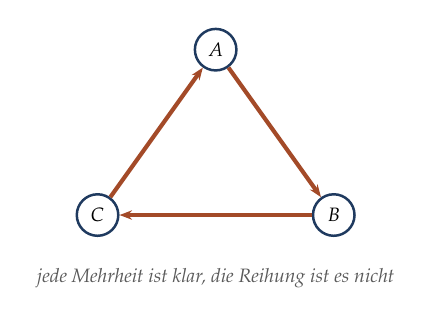
\begin{tikzpicture}[scale=1.0]
\node[knotenb] (A) at (0,1.3) {$A$};
\node[knotenb] (B) at (1.5,-0.8) {$B$};
\node[knotenb] (C) at (-1.5,-0.8) {$C$};
\draw[kanted, -{Stealth[length=4.5pt]}] (A)--(B);
\draw[kanted, -{Stealth[length=4.5pt]}] (B)--(C);
\draw[kanted, -{Stealth[length=4.5pt]}] (C)--(A);
\node[font=\scriptsize\itshape, color=grau] at (0,-1.6) {jede Mehrheit ist klar, die Reihung ist es nicht};
\end{tikzpicture}
\end{center}

\begin{center}
\begin{minipage}{0.9\textwidth}
\textbf{Die Mehrheitsreihung ist nicht übertragbar.} Es gibt keinen Sieger, obwohl jeder Einzelvergleich eindeutig ausgeht.
\end{minipage}
\end{center}

\begin{center}
\begin{minipage}{0.88\textwidth}
\kursiv{Die Übertragbarkeit war in Satz 4.1 eine Forderung an die Vorlieben des Einzelnen --- und jede Abteilung erfüllt sie hier. \textbf{Die Mehrheitsregel erhält sie nicht.} Das ist der Kern des Kapitels: Eine Eigenschaft, die alle Beteiligten haben, muss das Ergebnis der Zusammenführung nicht haben.}
\end{minipage}
\end{center}

\schritt{Die Folge für die Tagesordnung}
Stimmt man paarweise ab, so entscheidet die Reihenfolge der Abstimmungen.

\begin{center}
{\small
\renewcommand{\arraystretch}{1.5}
\begin{tabular}{@{}P{3.0cm}P{2.6cm}P{2.4cm}@{}}
\toprule
\textbf{Tagesordnung} & \textbf{erster Sieger} & \textbf{Ergebnis}\\
\midrule
erst $A$/$B$, dann gegen $C$ & $A$ & $C$\\
erst $B$/$C$, dann gegen $A$ & $B$ & $A$\\
erst $C$/$A$, dann gegen $B$ & $C$ & $B$\\
\bottomrule
\end{tabular}}
\end{center}

\begin{center}
\begin{minipage}{0.9\textwidth}
\textbf{Wer die Tagesordnung bestimmt, bestimmt das Ergebnis --- vollständig.}
\end{minipage}
\end{center}

\begin{center}
\begin{minipage}{0.88\textwidth}
\kursiv{Und zwar ohne jede Regelverletzung: Jede einzelne Abstimmung geht mit klarer Mehrheit aus. \textbf{Die Macht liegt bei der Sitzungsleitung, nicht bei den Stimmen} --- ein Befund, den jeder kennt, der Gremienarbeit betreibt, und der hier eine exakte Begründung erhält.}
\end{minipage}
\end{center}
\end{merksatz}

\section{Vier Verfahren, vier Sieger}

\begin{merksatz}
\boxtitel{Ein Beispiel mit fünf Geräten}
Dreiundfünfzig Stimmberechtigte, fünf Geräte:

\begin{center}
{\small
\renewcommand{\arraystretch}{1.5}
\begin{tabular}{@{}P{1.6cm}P{5.0cm}@{}}
\toprule
\textbf{Anzahl} & \textbf{Reihung}\\
\midrule
$18$ & $A \succ D \succ E \succ C \succ B$\\
$12$ & $B \succ E \succ D \succ C \succ A$\\
$10$ & $C \succ B \succ E \succ D \succ A$\\
$9$ & $D \succ C \succ E \succ B \succ A$\\
$4$ & $E \succ B \succ D \succ C \succ A$\\
\bottomrule
\end{tabular}}
\end{center}

\schritt{Verfahren 1 --- relative Mehrheit}
Nur der erste Platz zählt.
\begin{center}
{\small
\renewcommand{\arraystretch}{1.44}
\begin{tabular}{@{}P{1.2cm}P{1.2cm}P{1.2cm}P{1.2cm}P{1.2cm}@{}}
\toprule
$A$ & $B$ & $C$ & $D$ & $E$\\
$\mathbf{18}$ & $12$ & $10$ & $9$ & $4$\\
\bottomrule
\end{tabular}}
\end{center}
\[ \Longrightarrow\ A \]

\schritt{Verfahren 2 --- Stichwahl der beiden Besten}
$A$ gegen $B$:
\[ A: 18, \qquad B: 12+10+9+4 = 35 \]
\[ \Longrightarrow\ B \]

\schritt{Verfahren 3 --- schrittweise Ausscheidung}
Immer der Letzte fällt heraus, seine Stimmen gehen weiter.
\begin{center}
{\small
\renewcommand{\arraystretch}{1.44}
\begin{tabular}{@{}P{1.6cm}P{1.2cm}P{1.2cm}P{1.2cm}P{1.2cm}P{1.2cm}@{}}
\toprule
\textbf{Runde} & $A$ & $B$ & $C$ & $D$ & $E$\\
\midrule
$1$ & $18$ & $12$ & $10$ & $9$ & $4$\\
$2$ & $18$ & $16$ & $10$ & $9$ & ---\\
$3$ & $18$ & $16$ & $19$ & --- & ---\\
$4$ & $18$ & --- & $\mathbf{35}$ & & \\
\bottomrule
\end{tabular}}
\end{center}
\[ \Longrightarrow\ C \]

\schritt{Verfahren 4 --- Borda-Punkte}
Vier Punkte für den ersten Platz, drei für den zweiten, und so fort.
\begin{center}
{\small
\renewcommand{\arraystretch}{1.44}
\begin{tabular}{@{}P{1.2cm}P{1.4cm}P{1.4cm}P{1.4cm}P{1.4cm}P{1.4cm}@{}}
\toprule
& $A$ & $B$ & $C$ & $D$ & $E$\\
\midrule
Punkte & $72$ & $99$ & $101$ & $\mathbf{132}$ & $126$\\
\bottomrule
\end{tabular}}
\end{center}

\kursiv{Zur Spalte $D$:} $18\cdot3 + 12\cdot2 + 10\cdot1 + 9\cdot4 + 4\cdot2 = 54+24+10+36+8 = 132$

\[ \Longrightarrow\ D \]

\schritt{Verfahren 5 --- paarweise Mehrheiten}
$D$ schlägt jeden anderen:
\begin{center}
{\small
\renewcommand{\arraystretch}{1.46}
\begin{tabular}{@{}P{2.0cm}P{2.0cm}P{2.6cm}@{}}
\toprule
\textbf{Vergleich} & \textbf{Ergebnis} & \\
\midrule
$D$ gegen $A$ & $35:18$ & \\
$D$ gegen $B$ & $27:26$ & knapp\\
$D$ gegen $C$ & $43:10$ & \\
$D$ gegen $E$ & $27:26$ & knapp\\
\bottomrule
\end{tabular}}
\end{center}
\[ \Longrightarrow\ D \ \text{(Condorcet-Sieger)} \]

\begin{center}
\begin{minipage}{0.9\textwidth}
\textbf{Vier verschiedene Sieger bei fünf gebräuchlichen Verfahren --- aus denselben Stimmzetteln.}
\end{minipage}
\end{center}

\begin{center}
\begin{minipage}{0.88\textwidth}
\kursiv{Besonders unangenehm ist $A$: Es gewinnt die relative Mehrheit und verliert jeden Paarvergleich mit $18$ gegen $35$. \textbf{Achtzehn von dreiundfünfzig wollen $A$; fünfunddreißig halten es für das schlechteste.} Die relative Mehrheitswahl ist das einzige Verfahren, das diesen Umstand vollständig ignoriert --- und das am weitesten verbreitete.}
\end{minipage}
\end{center}
\end{merksatz}

\section{Der Satz von Arrow}

\begin{merksatz}
\boxtitel{Was man von einem Verfahren erwartet}
Ein \Begriff{Wahlverfahren} bildet die Reihungen aller Beteiligten auf eine gemeinsame Reihung ab.

\begin{center}
{\small
\renewcommand{\arraystretch}{1.55}
\begin{tabular}{@{}P{2.6cm}P{6.0cm}@{}}
\toprule
\textbf{Universalität} & Jede Zusammenstellung von Reihungen ist zulässig, und das Ergebnis ist stets eine vollständige, übertragbare Reihung.\\
\textbf{Einstimmigkeit} & Ziehen alle $x$ dem $y$ vor, so auch das Ergebnis.\\
\textbf{Unabhängigkeit} & Ob $x$ vor $y$ steht, hängt nur davon ab, wie die Beteiligten $x$ und $y$ zueinander reihen --- nicht von einer dritten Möglichkeit $z$.\\
\textbf{Keine Diktatur} & Es gibt keinen Beteiligten, dessen Reihung stets das Ergebnis ist.\\
\bottomrule
\end{tabular}}
\end{center}
\end{merksatz}

\begin{merksatz}
\boxtitel{Satz 12.1 --- Arrow, 1951}
Bei mindestens drei Möglichkeiten und mindestens zwei Beteiligten gibt es kein Verfahren, das alle vier Bedingungen erfüllt.

\begin{center}
\begin{minipage}{0.9\textwidth}
\textbf{Nicht: man kennt keines. Es gibt keines.}
\end{minipage}
\end{center}

\begin{center}
\begin{minipage}{0.88\textwidth}
\kursiv{Der Beweis ist nicht lang, aber trickreich; er führt über den Begriff einer entscheidenden Gruppe und zeigt, dass diese sich auf eine einzige Person zusammenziehen lässt. \textbf{Wir verzichten auf ihn} --- die zweite der neun Auslassungen dieses Bandes. Die Fundstelle ist Osborne und Rubinstein\zit{19}, Kapitel~10.}
\end{minipage}
\end{center}

\schritt{Wie die Verfahren scheitern}
\begin{center}
{\small
\renewcommand{\arraystretch}{1.5}
\begin{tabular}{@{}P{2.4cm}P{6.2cm}@{}}
\toprule
\textbf{Mehrheitsregel} & Verletzt die Universalität --- das Ergebnis ist nicht immer übertragbar (Abschnitt 12.2).\\
\textbf{Borda} & Verletzt die Unabhängigkeit --- eine zusätzliche Möglichkeit verschiebt die Punkte.\\
\textbf{Diktatur} & Erfüllt die ersten drei und ist ausgeschlossen.\\
\bottomrule
\end{tabular}}
\end{center}

\schritt{Die Unabhängigkeit ist die strittige Bedingung}
\begin{center}
\begin{minipage}{0.88\textwidth}
\kursiv{Sie verlangt, dass die Stärke einer Vorliebe unberücksichtigt bleibt --- ob jemand $x$ knapp oder deutlich vor $y$ setzt, darf keine Rolle spielen. \textbf{Genau das macht Borda anders}, und genau deshalb scheitert es an dieser Bedingung. Wer sie aufgibt, muss allerdings Nutzen zwischen Personen vergleichen, und Satz 4.1 sagt, dass das keinen Sinn ergibt.}
\end{minipage}
\end{center}
\end{merksatz}

\begin{merksatz}
\boxtitel{Satz 12.2 --- Gibbard und Satterthwaite, 1973/75}
Jedes Verfahren, das bei mindestens drei Möglichkeiten jede von ihnen erreichen kann und keine Diktatur ist, lässt sich durch falsche Angaben zum eigenen Vorteil beeinflussen.

\begin{center}
\begin{minipage}{0.9\textwidth}
\textbf{Es gibt kein Verfahren, bei dem ehrliches Abstimmen stets die beste Wahl ist.}
\end{minipage}
\end{center}

\begin{center}
\begin{minipage}{0.88\textwidth}
\kursiv{Der Satz ist eine Folgerung aus Satz 12.1 und in gewisser Weise die praktisch schärfere Aussage. \textbf{Arrow sagt, dass die Zusammenführung Mängel hat; Gibbard und Satterthwaite sagen, dass die Stimmzettel selbst unzuverlässig sind.} Wer taktisch abstimmt, gibt nicht seine Vorlieben an, und damit fehlt dem Verfahren die Eingabe, die es verarbeiten soll.}
\end{minipage}
\end{center}

\schritt{Borda wusste es}
\begin{center}
\begin{minipage}{0.88\textwidth}
\kursiv{Auf den Einwand, sein Verfahren lasse sich manipulieren, soll \Person{Jean-Charles de Borda} geantwortet haben, es sei nur für ehrliche Menschen gedacht. \textbf{Das ist keine Verteidigung, sondern eine Beschreibung der Lage} --- und Satz 12.2 besagt, dass es keinem anderen Verfahren besser ergeht.}
\end{minipage}
\end{center}
\end{merksatz}

\section{Der Bruchfall}

\begin{warnung}
\boxtitelr{Was die Sätze nicht bedeuten}
\begin{center}
{\small
\renewcommand{\arraystretch}{1.52}
\begin{tabular}{@{}P{2.4cm}P{6.2cm}@{}}
\toprule
\textbf{Nicht:} & \enquote{Alle Verfahren sind gleich schlecht.} Sie scheitern an verschiedenen Bedingungen und in verschieden häufigen Fällen.\\
\textbf{Nicht:} & \enquote{Abstimmen ist sinnlos.} Bei zwei Möglichkeiten gilt keiner der Sätze --- die einfache Mehrheit erfüllt alles.\\
\textbf{Nicht:} & \enquote{Manipulation ist häufig.} Sie ist möglich; ob sie gelingt, hängt davon ab, wie viel man über die anderen weiß.\\
\bottomrule
\end{tabular}}
\end{center}

\schritt{Zur zweiten Zeile}
\Person{Kenneth May} zeigte 1952, dass bei genau zwei Möglichkeiten die einfache Mehrheit das einzige Verfahren ist, das Gleichbehandlung der Stimmen, Gleichbehandlung der Möglichkeiten und Monotonie erfüllt.

\begin{center}
\begin{minipage}{0.88\textwidth}
\kursiv{\textbf{Die Schwierigkeit beginnt also exakt bei drei.} Das erklärt zugleich, warum Stichwahlen und Ausschussverfahren so verbreitet sind: Sie zerlegen die Aufgabe in Entscheidungen zwischen zweien --- um den Preis, dass die Reihenfolge das Ergebnis bestimmt, wie Abschnitt 12.2 zeigt.}
\end{minipage}
\end{center}

\schritt{Wie oft es überhaupt schiefgeht}
\begin{center}
{\small
\renewcommand{\arraystretch}{1.48}
\begin{tabular}{@{}P{2.6cm}P{2.2cm}P{3.0cm}@{}}
\toprule
\textbf{Möglich\-keiten} & \textbf{kein Sieger} & \\
\midrule
$3$ & $\approx 9\,\%$ & bei zufälligen Reihungen\\
$5$ & $\approx 25\,\%$ & \\
$10$ & $\approx 50\,\%$ & \\
\bottomrule
\end{tabular}}
\end{center}

\begin{center}
\begin{minipage}{0.88\textwidth}
\kursiv{Die Werte gelten für rein zufällige, voneinander unabhängige Reihungen und viele Stimmen --- der ungünstigste Fall. \textbf{In tatsächlichen Wahlen sind die Reihungen nicht zufällig}, sondern häufig entlang einer gemeinsamen Achse geordnet, und dann gibt es fast immer einen Sieger. Abschnitt 12.6 behandelt diesen Ausweg.}
\end{minipage}
\end{center}
\end{warnung}

\begin{merksatz}
\boxtitel{Der Ausweg: eingipflige Vorlieben}
Lassen sich die Möglichkeiten auf einer Linie anordnen, so dass jeder Beteiligte einen Bestpunkt hat und nach beiden Seiten hin abfällt, so heißen die Vorlieben \Begriff{eingipflig}.

\schritt{Satz 12.3 --- der Medianwähler, Black 1948}
Bei eingipfligen Vorlieben und ungerader Anzahl Beteiligter ist der Bestpunkt des mittleren Beteiligten ein Condorcet-Sieger.

\schritt{Beweis}
Sei $m$ der Median der Bestpunkte. Für jede Möglichkeit $y$ rechts von $m$ ziehen alle, deren Bestpunkt bei $m$ oder links davon liegt, $m$ dem $y$ vor --- das sind mindestens die Hälfte plus einer.

Ebenso für $y$ links von $m$. $\blacksquare$

\begin{center}
\begin{minipage}{0.9\textwidth}
\textbf{Eine Anordnung auf einer Linie genügt, und die Schwierigkeit verschwindet.}
\end{minipage}
\end{center}

\begin{center}
\begin{minipage}{0.88\textwidth}
\kursiv{Das erklärt, warum Abstimmungen über Beträge --- Budgethöhe, Personalschlüssel, Schwellenwerte --- meist glatt verlaufen: Sie sind von Natur aus eingipflig. \textbf{Schwierig wird es, wenn die Möglichkeiten sich in mehreren Hinsichten unterscheiden} --- etwa bei der Gerätewahl, wo Anschaffungspreis, Platzbedarf und Fachgebiet gegeneinanderstehen. Bei zwei oder mehr Dimensionen gilt der Satz nicht mehr.}
\end{minipage}
\end{center}
\end{merksatz}

\section{Übungsaufgaben}

\begin{aufgabe}
\boxtitel{Aufgabe 12.1 --- Ein Verfahren wählen}
Prüfen Sie am Beispiel aus Abschnitt 12.3, welches Gerät jedes Verfahren wählt, und beurteilen Sie die Ergebnisse.

\loesung
\schritt{Schritt 1 --- Die Übersicht}
\begin{center}
{\small
\renewcommand{\arraystretch}{1.5}
\begin{tabular}{@{}P{3.0cm}P{1.4cm}P{3.0cm}@{}}
\toprule
\textbf{Verfahren} & \textbf{Sieger} & \\
\midrule
relative Mehrheit & $A$ & \\
Zweierstichwahl & $B$ & \\
Ausscheidung & $C$ & \\
Borda & $D$ & \\
Paarvergleich & $D$ & Condorcet-Sieger\\
\bottomrule
\end{tabular}}
\end{center}

\schritt{Schritt 2 --- $A$ beurteilen}
\[ A \ \text{gegen jeden anderen}: 18:35 \]

\begin{center}
\begin{minipage}{0.9\textwidth}
\textbf{$A$ verliert jeden Paarvergleich --- es ist ein Condorcet-Verlierer.}
\end{minipage}
\end{center}

\kursiv{Grund:} Alle $35$ Stimmberechtigten, die $A$ nicht auf Platz eins setzen, setzen es auf Platz fünf.

\schritt{Schritt 3 --- $C$ beurteilen}
\begin{center}
\renewcommand{\arraystretch}{1.48}
\begin{tabular}{@{}P{2.4cm}P{2.0cm}P{2.6cm}@{}}
\toprule
\textbf{Vergleich} & \textbf{Ergebnis} & \\
\midrule
$C$ gegen $D$ & $10:43$ & deutlich verloren\\
$C$ gegen $E$ & $19:34$ & verloren\\
$C$ gegen $B$ & $37:16$ & gewonnen\\
\bottomrule
\end{tabular}
\end{center}

\begin{center}
\begin{minipage}{0.9\textwidth}
\textbf{Das Ausscheidungsverfahren wählt ein Gerät, das gegen $D$ mit $10$ zu $43$ verliert.}
\end{minipage}
\end{center}

\begin{center}
\begin{minipage}{0.88\textwidth}
\kursiv{Das ist kein Randfall dieses Beispiels, sondern eine bekannte Eigenschaft: \textbf{Das Ausscheidungsverfahren kann den Condorcet-Sieger in einer frühen Runde eliminieren}, weil es nur erste Plätze zählt. $D$ hatte nur neun erste Plätze und wurde in Runde 3 ausgeschieden --- obwohl es gegen alle anderen eine Mehrheit hat.}
\end{minipage}
\end{center}

\schritt{Schritt 4 --- $D$ beurteilen}
\begin{center}
\begin{minipage}{0.9\textwidth}
\textbf{$D$ schlägt jeden anderen in der direkten Abstimmung --- zweimal allerdings nur mit $27$ zu $26$.}
\end{minipage}
\end{center}

\begin{center}
\begin{minipage}{0.88\textwidth}
\kursiv{Die Knappheit gegen $B$ und gegen $E$ ist bemerkenswert. \textbf{Ein Condorcet-Sieger ist nicht notwendig ein starker Sieger}, sondern nur einer, der keinen Paarvergleich verliert. Eine einzige Stimmänderung könnte die Lage kippen --- und dann gäbe es keinen Condorcet-Sieger mehr.}
\end{minipage}
\end{center}

\schritt{Schritt 5 --- Die Empfehlung}
\begin{center}
{\small
\renewcommand{\arraystretch}{1.5}
\begin{tabular}{@{}P{2.4cm}P{6.2cm}@{}}
\toprule
\textbf{Wenn es einen gibt} & Der Condorcet-Sieger ist die sicherste Wahl --- keine Mehrheit zieht etwas anderes vor.\\
\textbf{Wenn nicht} & Borda liefert ein plausibles Ergebnis und schließt den Condorcet-Verlierer aus; manipulierbar bleibt es.\\
\textbf{Nie} & Die relative Mehrheit bei mehr als zwei Möglichkeiten.\\
\bottomrule
\end{tabular}}
\end{center}

\begin{center}
\begin{minipage}{0.88\textwidth}
\kursiv{Der letzte Punkt ist die einzige klare Handlungsempfehlung, die dieses Kapitel hergibt. \textbf{Sie folgt nicht aus Arrow, sondern aus der Anschauung}: Ein Verfahren, das den Condorcet-Verlierer zum Sieger erklären kann, ist schwer zu rechtfertigen.}
\end{minipage}
\end{center}
\end{aufgabe}

\begin{aufgabe}
\boxtitel{Aufgabe 12.2 --- Die Tagesordnung nutzen}
Im Paradoxon aus Abschnitt 12.2 leitet die Radiologie die Sitzung und möchte, dass $C$ gewinnt. Welche Tagesordnung wählt sie?

\loesung
\schritt{Schritt 1 --- Die Zyklusrichtung}
\[ A \succ B, \qquad B \succ C, \qquad C \succ A \]

\schritt{Schritt 2 --- Der Gedanke}
Die eigene Möglichkeit soll \kursiv{zuletzt} antreten, gegen denjenigen, den sie schlägt.

\[ C \ \text{schlägt} \ A \quad\Longrightarrow\quad A \ \text{muss die erste Runde gewinnen} \]

\schritt{Schritt 3 --- Die Tagesordnung}
\begin{center}
{\small
\renewcommand{\arraystretch}{1.5}
\begin{tabular}{@{}P{1.8cm}P{2.8cm}P{2.6cm}@{}}
\toprule
\textbf{Runde} & \textbf{Abstimmung} & \textbf{Sieger}\\
\midrule
$1$ & $A$ gegen $B$ & $A$ $(2:1)$\\
$2$ & $A$ gegen $C$ & $\mathbf{C}$ $(2:1)$\\
\bottomrule
\end{tabular}}
\end{center}

\schritt{Schritt 4 --- Die Probe für die anderen}
\begin{center}
{\small
\renewcommand{\arraystretch}{1.5}
\begin{tabular}{@{}P{2.6cm}P{2.4cm}P{2.4cm}@{}}
\toprule
\textbf{Wer leitet} & \textbf{Erste Runde} & \textbf{Ergebnis}\\
\midrule
Chirurgie ($A$) & $B$ gegen $C$ & $A$\\
Innere ($B$) & $C$ gegen $A$ & $B$\\
Radiologie ($C$) & $A$ gegen $B$ & $C$\\
\bottomrule
\end{tabular}}
\end{center}

\begin{center}
\begin{minipage}{0.9\textwidth}
\textbf{Jede Abteilung kann ihr eigenes Gerät durchsetzen, wenn sie die Tagesordnung bestimmt.}
\end{minipage}
\end{center}

\schritt{Schritt 5 --- Die Regel}
\begin{center}
\begin{minipage}{0.9\textwidth}
\textbf{Die eigene Möglichkeit in die letzte Runde --- und als Gegner denjenigen, den sie schlägt.}
\end{minipage}
\end{center}

\begin{center}
\begin{minipage}{0.88\textwidth}
\kursiv{Wer zuerst antritt, muss zweimal gewinnen; wer zuletzt antritt, nur einmal. \textbf{Das ist der Spätzieher-Vorteil} --- und damit das Gegenstück zum Erstzieher-Vorteil aus Kapitel~7. Ob Früh oder Spät nützt, hängt daran, ob man festlegt oder antwortet.}
\end{minipage}
\end{center}

\schritt{Schritt 6 --- Die Gegenmaßnahme}
\begin{center}
{\small
\renewcommand{\arraystretch}{1.5}
\begin{tabular}{@{}P{2.4cm}P{6.2cm}@{}}
\toprule
\textbf{Alle Paare} & Man stimmt über sämtliche Paare ab und sucht den Condorcet-Sieger. Gibt es keinen, ist das sichtbar.\\
\textbf{Borda} & Kennt keine Tagesordnung.\\
\textbf{Losentscheid} & Bei nachgewiesenem Zyklus --- unbefriedigend, aber unparteiisch.\\
\bottomrule
\end{tabular}}
\end{center}

\begin{center}
\begin{minipage}{0.88\textwidth}
\kursiv{Die erste Zeile ist bei wenigen Möglichkeiten praktikabel: Bei $k$ Möglichkeiten sind $\binom k2$ Abstimmungen nötig, bei fünf also zehn. \textbf{Der Aufwand verhindert die Manipulation der Reihenfolge vollständig} --- und macht zugleich sichtbar, wenn kein Sieger existiert. Das ist mehr wert als ein Ergebnis, das nur so aussieht, als wäre es eines.}
\end{minipage}
\end{center}
\end{aufgabe}

\begin{aufgabe}
\boxtitel{Aufgabe 12.3 --- Taktisch abstimmen}
Beim Borda-Verfahren im kleinen Beispiel --- $5$ mit $A\succ B\succ C$, $4$ mit $B\succ C\succ A$, $3$ mit $C\succ B\succ A$ --- können die $A$-Anhänger ihre Stimmzettel ändern. Was erreichen sie?

\loesung
\schritt{Schritt 1 --- Das ehrliche Ergebnis}
Punkte $2$, $1$, $0$:
\begin{center}
{\small
\renewcommand{\arraystretch}{1.48}
\begin{tabular}{@{}P{1.6cm}P{3.2cm}P{1.6cm}@{}}
\toprule
& \textbf{Rechnung} & \textbf{Summe}\\
\midrule
$A$ & $5\cdot2$ & $10$\\
$B$ & $5\cdot1+4\cdot2+3\cdot1$ & $\mathbf{16}$\\
$C$ & $4\cdot1+3\cdot2$ & $10$\\
\bottomrule
\end{tabular}}
\end{center}

$B$ gewinnt; die $A$-Anhänger erhalten ihre zweite Wahl.

\schritt{Schritt 2 --- Der Eingriff}
Die fünf $A$-Anhänger geben statt $A\succ B\succ C$ nun $A\succ C\succ B$ an --- sie stufen den gefährlichsten Gegner herab.

\begin{center}
{\small
\renewcommand{\arraystretch}{1.48}
\begin{tabular}{@{}P{1.6cm}P{3.2cm}P{1.6cm}@{}}
\toprule
& \textbf{Rechnung} & \textbf{Summe}\\
\midrule
$A$ & $5\cdot2$ & $10$\\
$B$ & $5\cdot0+4\cdot2+3\cdot1$ & $11$\\
$C$ & $5\cdot1+4\cdot1+3\cdot2$ & $\mathbf{15}$\\
\bottomrule
\end{tabular}}
\end{center}

\begin{center}
\begin{minipage}{0.9\textwidth}
\textbf{Nun gewinnt $C$ --- die \kursiv{letzte} Wahl der $A$-Anhänger.} Der Eingriff hat ihnen geschadet.
\end{minipage}
\end{center}

\schritt{Schritt 3 --- Der bessere Eingriff}
Um $A$ zum Sieg zu verhelfen, müssten die $A$-Anhänger $A$ um mindestens sieben Punkte verbessern --- das geht nicht, denn $A$ steht bei ihnen bereits ganz oben.

\begin{center}
\begin{minipage}{0.9\textwidth}
\textbf{$A$ ist nicht durchsetzbar.} Die einzige Frage ist, ob $B$ oder $C$ gewinnt.
\end{minipage}
\end{center}

\kursiv{Da die $A$-Anhänger $B$ dem $C$ vorziehen, ist ehrliches Abstimmen hier die beste Wahl.}

\schritt{Schritt 4 --- Wo der Eingriff lohnt}
Die $C$-Anhänger ($3$ Stimmen) geben statt $C\succ B\succ A$ nun $C\succ A\succ B$ an:
\begin{center}
{\small
\renewcommand{\arraystretch}{1.48}
\begin{tabular}{@{}P{1.6cm}P{3.2cm}P{1.6cm}@{}}
\toprule
& \textbf{Rechnung} & \textbf{Summe}\\
\midrule
$A$ & $5\cdot2+3\cdot1$ & $13$\\
$B$ & $5\cdot1+4\cdot2$ & $13$\\
$C$ & $4\cdot1+3\cdot2$ & $10$\\
\bottomrule
\end{tabular}}
\end{center}

\begin{center}
\begin{minipage}{0.9\textwidth}
\textbf{Gleichstand zwischen $A$ und $B$ --- und die $C$-Anhänger ziehen $B$ dem $A$ vor.} Auch dieser Eingriff schadet.
\end{minipage}
\end{center}

\schritt{Schritt 5 --- Der Fall, in dem es gelingt}
Die vier $B$-Anhänger stufen $C$ herab: statt $B\succ C\succ A$ nun $B\succ A\succ C$.
\begin{center}
{\small
\renewcommand{\arraystretch}{1.48}
\begin{tabular}{@{}P{1.6cm}P{3.2cm}P{1.6cm}@{}}
\toprule
& \textbf{Rechnung} & \textbf{Summe}\\
\midrule
$A$ & $5\cdot2+4\cdot1$ & $14$\\
$B$ & $5\cdot1+4\cdot2+3\cdot1$ & $\mathbf{16}$\\
$C$ & $3\cdot2$ & $6$\\
\bottomrule
\end{tabular}}
\end{center}

$B$ gewinnt weiterhin --- hier war der Eingriff unnötig, aber ungefährlich.

\schritt{Schritt 6 --- Die Lehre}
\begin{center}
\begin{minipage}{0.88\textwidth}
\kursiv{Satz 12.2 besagt, dass es \kursiv{Stimmenverteilungen} gibt, bei denen sich falsche Angaben lohnen --- nicht, dass es bei jeder Verteilung so ist. \textbf{In diesem Beispiel schadet der Eingriff jedem, der ihn versucht}, weil $B$ eine so breite Zustimmung hat. Manipulierbarkeit ist eine Eigenschaft des Verfahrens; ob sich Manipulation lohnt, hängt an den Stimmen --- und an dem, was man über sie weiß.}
\end{minipage}
\end{center}
\end{aufgabe}

\begin{geschichte}
\boxtitelg{Zwei Franzosen und ein Amerikaner}
\Person{Jean-Charles de Borda} (1733--1799) schlug sein Punkteverfahren 1770 der Académie des Sciences vor, die es zur Wahl ihrer Mitglieder übernahm.

\begin{center}
\begin{minipage}{0.9\textwidth}
\kursiv{Die Akademie behielt es bis 1800 bei. Dann wurde es auf Betreiben eines neuen Mitglieds abgeschafft --- \Person{Napoleon Bonaparte}, der als Erster Konsul den Vorsitz übernommen hatte. \textbf{Die Begründung ist nicht überliefert.}}
\end{minipage}
\end{center}

\schritt{Condorcet}
\Person{Nicolas de Condorcet} (1743--1794) wies 1785 auf das nach ihm benannte Paradoxon hin und schlug die paarweise Abstimmung vor.

\begin{center}
\begin{minipage}{0.9\textwidth}
\kursiv{Er war Mathematiker, Philosoph und Politiker, verfasste einen Verfassungsentwurf für die Republik und setzte sich früh für die Gleichberechtigung von Frauen und für die Abschaffung der Sklaverei ein. \textbf{Er starb 1794 in einer Gefängniszelle}, nachdem er als Girondist geächtet worden war --- die Umstände sind ungeklärt.}
\end{minipage}
\end{center}

\schritt{Die Wiederentdeckung}
Beide Arbeiten gerieten in Vergessenheit. \Person{Charles Dodgson} --- besser bekannt als \Person{Lewis Carroll} --- entwickelte in den 1870er Jahren unabhängig verwandte Verfahren für die Wahlen seines Colleges.

\begin{center}
\begin{minipage}{0.9\textwidth}
\kursiv{\Person{Duncan Black} stellte in den 1940er Jahren die Zusammenhänge her und bewies den Satz über den Medianwähler. \textbf{Er entdeckte dabei Condorcets und Bordas Arbeiten wieder}, die über anderthalb Jahrhunderte unbeachtet geblieben waren.}
\end{minipage}
\end{center}

\schritt{Arrow}
\Person{Kenneth Arrow} (1921--2017) bewies seinen Satz 1950 als Doktorand, im Alter von neunundzwanzig Jahren.

\begin{center}
\begin{minipage}{0.9\textwidth}
\kursiv{Er hatte nach einem Verfahren gesucht und stattdessen bewiesen, dass es keines gibt. \textbf{Die Arbeit umfasst in Buchform gut hundert Seiten} und begründete ein eigenes Fach, die Theorie der gesellschaftlichen Wahl. 1972 erhielt Arrow den Wirtschaftsnobelpreis --- als bis heute jüngster Träger.}
\end{minipage}
\end{center}
\end{geschichte}

\begin{forschung}
\boxtitelp{Wahlverfahren heute}
\begin{center}
{\small
\renewcommand{\arraystretch}{1.45}
\begin{tabular}{@{}P{3.2cm}P{5.0cm}@{}}
\toprule
\textbf{Im Einsatz} & Ausscheidungsverfahren in Australien und Irland, seit 2018 auch in mehreren amerikanischen Städten.\\
\textbf{Zustimmungs\-wahl} & Jeder kreuzt beliebig viele an; umgeht Arrow, weil keine Reihung verlangt wird.\\
\textbf{Rechenaufwand} & Manche Verfahren sind nachweislich schwer manipulierbar --- ein Schutz durch Komplexität.\\
\bottomrule
\end{tabular}}
\end{center}

\schritt{Zur zweiten Zeile}
Bei der Zustimmungswahl gibt jeder an, welche Möglichkeiten er für annehmbar hält.

\begin{center}
\begin{minipage}{0.88\textwidth}
\kursiv{Satz 12.1 setzt voraus, dass Reihungen die Eingabe sind --- daher greift er hier nicht unmittelbar. \textbf{Dafür entsteht ein neues Problem: Wo setzt man die Grenze?} Die Antwort hängt davon ab, was man über die anderen erwartet, und damit ist das taktische Element zurück. Satz 12.2 gilt für die Zustimmungswahl ebenfalls.}
\end{minipage}
\end{center}

\schritt{Zur dritten Zeile}
Für einige Verfahren ist die Berechnung einer wirksamen Manipulation $\mathsf{NP}$-schwer.

\begin{center}
\begin{minipage}{0.88\textwidth}
\kursiv{Das klingt nach einem Ausweg und ist in der Praxis schwächer, als es aussieht: \textbf{Die Schwere gilt für den schlechtesten Fall}, und die häufig auftretenden Stimmenverteilungen sind oft leicht zu manipulieren. Es ist dasselbe Problem wie in Band 20, Kapitel~10 --- ein Verfahren, dessen Sicherheit an einer Worst-Case-Aussage hängt, ist nicht solide.}
\end{minipage}
\end{center}
\end{forschung}

\begin{merksatz}
\boxtitel{Was Sie jetzt können}
\begin{center}
\renewcommand{\arraystretch}{1.5}
\begin{tabular}{@{}P{3.0cm}P{5.6cm}@{}}
\toprule
\textbf{Condorcet} & Mehrheiten sind nicht übertragbar\\
\textbf{Die Tagesordnung} & entscheidet vollständig\\
\textbf{Satz 12.1} & Arrow: es gibt kein Verfahren\\
\textbf{Satz 12.2} & keines ist manipulationsfest\\
\textbf{Satz 12.3} & eingipflig: der Median gewinnt\\
\bottomrule
\end{tabular}
\end{center}

\begin{center}
\begin{minipage}{0.88\textwidth}
\kursiv{Arrow verlangt eine vollständige Reihung als Ergebnis. Das nächste Kapitel verlangt weniger --- nur eine Zuteilung --- und findet Verfahren, die tatsächlich funktionieren.}
\end{minipage}
\end{center}
\end{merksatz}

\chapter{Auktionen und Zuteilung}

\section{Was Kapitel 12 übrig lässt}

\begin{merksatz}
\boxtitel{Die Forderung abschwächen}
Arrow verlangt eine vollständige Reihung aller Möglichkeiten als Ergebnis. Meist braucht man weniger.

\begin{center}
{\small
\renewcommand{\arraystretch}{1.5}
\begin{tabular}{@{}P{2.4cm}P{6.2cm}@{}}
\toprule
\textbf{Kapitel 12} & \enquote{Wie ordnen wir alle Geräte?}\\
\textbf{Hier} & \enquote{Wer bekommt den Auftrag?} und \enquote{Wer bekommt welche Stelle?}\\
\bottomrule
\end{tabular}}
\end{center}

\begin{center}
\begin{minipage}{0.9\textwidth}
\textbf{Eine Zuteilung ist keine Reihung --- und dafür gibt es Verfahren, die funktionieren.}
\end{minipage}
\end{center}

\schritt{Zwei Leitfälle}
\begin{center}
{\small
\renewcommand{\arraystretch}{1.5}
\begin{tabular}{@{}P{2.4cm}P{6.2cm}@{}}
\toprule
\textbf{Mit Geld} & Das Klinikum schreibt einen Wartungsvertrag aus. Die Bieter kennen ihre Kosten, das Klinikum nicht.\\
\textbf{Ohne Geld} & Weiterbildungsstellen werden an Bewerber vergeben. Beide Seiten haben Vorlieben.\\
\bottomrule
\end{tabular}}
\end{center}
\end{merksatz}

\section{Vier Auktionsformen}

\begin{merksatz}
\boxtitel{Die gebräuchlichen Formen}
\begin{center}
{\small
\renewcommand{\arraystretch}{1.52}
\begin{tabular}{@{}P{2.4cm}P{6.2cm}@{}}
\toprule
\textbf{Englisch} & Der Preis steigt, bis nur einer bleibt. Offen.\\
\textbf{Holländisch} & Der Preis fällt, bis der Erste zugreift. Offen.\\
\textbf{Erstpreis} & Verdeckte Gebote; der Höchstbietende zahlt sein Gebot.\\
\textbf{Zweitpreis} & Verdeckte Gebote; der Höchstbietende zahlt das \kursiv{zweithöchste} Gebot.\\
\bottomrule
\end{tabular}}
\end{center}

\begin{center}
\begin{minipage}{0.9\textwidth}
\textbf{Die vierte Form wirkt widersinnig --- der Verkäufer verschenkt die Differenz.} Sie ist die einzige, bei der ehrliches Bieten stets richtig ist.
\end{minipage}
\end{center}

\schritt{Die Paarungen}
\begin{center}
{\small
\renewcommand{\arraystretch}{1.5}
\begin{tabular}{@{}P{2.6cm}P{6.0cm}@{}}
\toprule
\textbf{Holländisch} & entspricht der Erstpreisauktion: Man muss vorab festlegen, bei welchem Preis man zugreift --- ohne etwas über die anderen zu erfahren.\\
\textbf{Englisch} & entspricht der Zweitpreisauktion: Man bleibt bis zum eigenen Wert und zahlt das, was der Vorletzte geboten hat.\\
\bottomrule
\end{tabular}}
\end{center}

\begin{center}
\begin{minipage}{0.88\textwidth}
\kursiv{Die zweite Paarung erklärt, warum die Zweitpreisauktion weniger seltsam ist, als sie aussieht: \textbf{Jede gewöhnliche Versteigerung ist eine} --- der Zuschlag erfolgt knapp über dem Gebot des vorletzten Bieters, nicht bei der Zahlungsbereitschaft des Siegers.}
\end{minipage}
\end{center}
\end{merksatz}

\section{Die Zweitpreisauktion}

\begin{merksatz}
\boxtitel{Satz 13.1 --- Vickrey, 1961}
In der Zweitpreisauktion ist das Bieten des eigenen Wertes eine schwach dominante Strategie.

\schritt{Beweis}
Sei $v$ mein Wert, $b$ mein Gebot und $m$ das höchste Gebot der anderen. Mein Nutzen beträgt $v-m$, wenn ich gewinne, sonst null.

\kursiv{Fall 1: $b > v$.} Das ändert nur etwas, wenn $m$ zwischen $v$ und $b$ liegt. Dann gewinne ich und zahle $m > v$:
\[ v - m \ <\ 0 . \]
Mit $b=v$ hätte ich verloren und null erhalten. \textbf{Schlechter.}

\kursiv{Fall 2: $b < v$.} Das ändert nur etwas, wenn $m$ zwischen $b$ und $v$ liegt. Dann verliere ich und erhalte null, statt
\[ v - m \ >\ 0 \]
zu bekommen. \textbf{Schlechter.}

\kursiv{In allen übrigen Fällen} ist das Ergebnis dasselbe wie bei $b=v$. $\blacksquare$

\begin{center}
\begin{minipage}{0.9\textwidth}
\textbf{Man braucht nichts über die anderen zu wissen.} Der eigene Wert genügt --- das ist Dominanz im Sinne von Kapitel~1.
\end{minipage}
\end{center}

\schritt{Die Zahlen}
Bei $v = 100$:
\begin{center}
{\small
\renewcommand{\arraystretch}{1.48}
\begin{tabular}{@{}P{1.6cm}P{1.8cm}P{2.0cm}P{2.0cm}@{}}
\toprule
\textbf{Gebot} & \textbf{fremdes} & \textbf{Ausgang} & \textbf{Nutzen}\\
\midrule
$100$ & $80$ & gewinnt & $+20$\\
$120$ & $110$ & gewinnt & $\mathbf{-10}$\\
$120$ & $90$ & gewinnt & $+10$\\
$80$ & $90$ & \textcolor{akzent}{verliert} & $\mathbf{0}$\\
$80$ & $70$ & gewinnt & $+30$\\
\bottomrule
\end{tabular}}
\end{center}

\begin{center}
\begin{minipage}{0.88\textwidth}
\kursiv{Die zweite Zeile zeigt den Schaden des Überbietens, die vierte den des Unterbietens: Bei einem fremden Gebot von $90$ hätte man mit $100$ gewonnen und $10$ verdient. \textbf{Die dritte und die fünfte Zeile sind dieselben wie bei ehrlichem Gebot} --- das Überbieten schadet nur dort, wo es überhaupt wirkt.}
\end{minipage}
\end{center}
\end{merksatz}

\begin{merksatz}
\boxtitel{Die Erstpreisauktion}
Hier lohnt ehrliches Bieten nicht: Wer seinen Wert bietet, gewinnt ohne Gewinn.

\schritt{Das Gleichgewichtsgebot}
Bei $n$ Bietern mit unabhängigen, auf $[0,1]$ gleichverteilten Werten lautet es
\[ b(v) = \frac{n-1}{n}\,v . \]

\begin{center}
{\small
\renewcommand{\arraystretch}{1.48}
\begin{tabular}{@{}P{1.6cm}P{2.2cm}P{3.0cm}@{}}
\toprule
$n$ & \textbf{Anteil} & \\
\midrule
$2$ & $50\,\%$ & die Hälfte des Wertes\\
$3$ & $67\,\%$ & \\
$5$ & $80\,\%$ & \\
$10$ & $90\,\%$ & \\
\bottomrule
\end{tabular}}
\end{center}

\begin{center}
\begin{minipage}{0.9\textwidth}
\textbf{Je mehr Bieter, desto näher am eigenen Wert.} Der Wettbewerb zwingt zur Offenheit.
\end{minipage}
\end{center}

\begin{center}
\begin{minipage}{0.88\textwidth}
\kursiv{Man beachte, was hier verlangt wird: Der Bieter muss $n$ kennen und die Verteilung der fremden Werte. \textbf{Bei der Zweitpreisauktion braucht er nichts davon} --- das ist der eigentliche Vorzug, nicht der Preis.}
\end{minipage}
\end{center}
\end{merksatz}

\begin{merksatz}
\boxtitel{Satz 13.2 --- die Erlösgleichheit}
Unter den genannten Annahmen erbringen alle vier Formen denselben erwarteten Erlös:
\[ \mathbb{E}[\text{Erlös}] = \frac{n-1}{n+1} . \]

\schritt{Die Rechnung für die Zweitpreisauktion}
Der Erlös ist der zweithöchste Wert. Für $n$ gleichverteilte Werte gilt
\[ \mathbb{E}\bigl[v_{(n-1)}\bigr] = \frac{n-1}{n+1} . \]

\schritt{Die Rechnung für die Erstpreisauktion}
Der Erlös ist das Gebot des Höchstbietenden:
\[ \mathbb{E}\left[\frac{n-1}{n}\,v_{(n)}\right] = \frac{n-1}{n}\cdot\frac{n}{n+1} = \frac{n-1}{n+1} \quad \checkmark \]

\begin{center}
{\small
\renewcommand{\arraystretch}{1.48}
\begin{tabular}{@{}P{1.6cm}P{2.0cm}P{2.0cm}P{1.8cm}@{}}
\toprule
$n$ & \textbf{Zweitpreis} & \textbf{Erstpreis} & \\
\midrule
$2$ & $0{,}3333$ & $0{,}3333$ & \\
$3$ & $0{,}5000$ & $0{,}5000$ & \\
$5$ & $0{,}6667$ & $0{,}6667$ & \\
$10$ & $0{,}8182$ & $0{,}8182$ & \\
\bottomrule
\end{tabular}}
\end{center}

\kursiv{Probe durch Simulation, $n=3$, $200\,000$ Durchläufe:} $0{,}5002$ und $0{,}4997$. \checkmark

\begin{center}
\begin{minipage}{0.9\textwidth}
\textbf{Die Wahl der Auktionsform ändert den erwarteten Erlös nicht --- nur, wie die Bieter sich verhalten.}
\end{minipage}
\end{center}

\begin{center}
\begin{minipage}{0.88\textwidth}
\kursiv{Das ist ein überraschendes und zugleich zerbrechliches Ergebnis. \textbf{Es gilt nur unter den genannten Annahmen}: unabhängige private Werte, risikoneutrale Bieter, symmetrische Verteilung, keine Absprachen. Wird eine davon verletzt, trennen sich die Formen --- und der Bruchfall zeigt, wie weit.}
\end{minipage}
\end{center}
\end{merksatz}

\section{Zuteilung ohne Geld}

\begin{merksatz}
\boxtitel{Der Leitfall: Weiterbildungsstellen}
Drei Bewerber, drei Kliniken, jede Seite mit Vorlieben.

\begin{center}
{\small
\renewcommand{\arraystretch}{1.5}
\begin{tabular}{@{}P{2.0cm}P{2.8cm}P{2.0cm}P{2.8cm}@{}}
\toprule
\textbf{Arzt} & \textbf{Reihung} & \textbf{Klinik} & \textbf{Reihung}\\
\midrule
$a_1$ & $K_1 \succ K_2 \succ K_3$ & $K_1$ & $a_2 \succ a_3 \succ a_1$\\
$a_2$ & $K_2 \succ K_3 \succ K_1$ & $K_2$ & $a_3 \succ a_1 \succ a_2$\\
$a_3$ & $K_3 \succ K_1 \succ K_2$ & $K_3$ & $a_1 \succ a_2 \succ a_3$\\
\bottomrule
\end{tabular}}
\end{center}
\end{merksatz}

\begin{definition}
\boxtitelm{Definition 13.3 --- stabil}
Eine Zuordnung heißt \Begriff{stabil}, wenn es kein Paar gibt, das einander dem Zugeteilten vorzieht.
\end{definition}

\begin{merksatz}
\boxtitel{Das Verfahren von Gale und Shapley}
\begin{center}
{\small
\renewcommand{\arraystretch}{1.5}
\begin{tabular}{@{}P{1.0cm}P{7.4cm}@{}}
\toprule
$1$ & Jeder noch nicht vorläufig Zugeordnete fragt bei seiner besten noch nicht abgelehnten Stelle an.\\
$2$ & Jede Stelle behält vorläufig den besten Anfragenden und lehnt die übrigen ab.\\
$3$ & Wiederholen, bis niemand mehr frei ist.\\
\bottomrule
\end{tabular}}
\end{center}

\schritt{Satz 13.4 --- Gale und Shapley, 1962}
\begin{center}
{\small
\renewcommand{\arraystretch}{1.52}
\begin{tabular}{@{}P{2.4cm}P{6.2cm}@{}}
\toprule
\textbf{Es endet} & Nach höchstens $n^{2}$ Anfragen, denn keine Stelle wird zweimal gefragt.\\
\textbf{Es ist stabil} & Kein Paar zieht einander vor.\\
\textbf{Einseitig bestes} & Die anfragende Seite erhält unter allen stabilen Zuordnungen ihre beste.\\
\bottomrule
\end{tabular}}
\end{center}

\schritt{Beweis der Stabilität}
Angenommen, $a$ zieht $K$ seiner Zuteilung vor und $K$ zieht $a$ der ihren vor.

Da $a$ die Stellen der Reihe nach durchgeht und $K$ besser ist als die erhaltene, hat $a$ bei $K$ angefragt --- und wurde abgelehnt.

$K$ lehnt nur ab, wenn sie jemand Besseren hält. Da $K$ im Verlauf nur besser wird, hält sie am Ende jemanden, den sie $a$ vorzieht. \textbf{Widerspruch.} $\blacksquare$
\end{merksatz}

\begin{merksatz}
\boxtitel{Der Leitfall gerechnet}
\schritt{Wenn die Ärzte anfragen}
\begin{center}
{\small
\renewcommand{\arraystretch}{1.48}
\begin{tabular}{@{}P{2.0cm}P{2.4cm}P{2.6cm}@{}}
\toprule
\textbf{Anfrage} & \textbf{Antwort} & \\
\midrule
$a_1 \to K_1$ & angenommen & \\
$a_2 \to K_2$ & angenommen & \\
$a_3 \to K_3$ & angenommen & \\
\bottomrule
\end{tabular}}
\end{center}

\[ a_1\!-\!K_1, \quad a_2\!-\!K_2, \quad a_3\!-\!K_3 \]

\begin{center}
\begin{minipage}{0.9\textwidth}
\textbf{Jeder Arzt erhält seine erste Wahl --- jede Klinik ihre letzte.}
\end{minipage}
\end{center}

\schritt{Wenn die Kliniken anfragen}
\begin{center}
{\small
\renewcommand{\arraystretch}{1.48}
\begin{tabular}{@{}P{2.0cm}P{2.4cm}P{2.6cm}@{}}
\toprule
\textbf{Anfrage} & \textbf{Antwort} & \\
\midrule
$K_1 \to a_2$ & angenommen & \\
$K_2 \to a_3$ & angenommen & \\
$K_3 \to a_1$ & angenommen & \\
\bottomrule
\end{tabular}}
\end{center}

\[ a_2\!-\!K_1, \quad a_3\!-\!K_2, \quad a_1\!-\!K_3 \]

\begin{center}
\begin{minipage}{0.9\textwidth}
\textbf{Nun erhält jede Klinik ihre erste Wahl --- jeder Arzt seine letzte.}
\end{minipage}
\end{center}

\schritt{Beide sind stabil}
\kursiv{Prüfung der zweiten Zuordnung:} $a_1$ hätte lieber $K_1$ --- aber $K_1$ hat $a_2$ und zieht $a_2$ dem $a_1$ vor. Ebenso für $K_2$ und $a_3$. Kein blockierendes Paar. \checkmark

\begin{center}
{\small
\renewcommand{\arraystretch}{1.5}
\begin{tabular}{@{}P{2.6cm}P{2.4cm}P{2.6cm}@{}}
\toprule
& \textbf{Ärzte} & \textbf{Kliniken}\\
\midrule
Ärzte fragen & Rang $1$ & Rang $3$\\
Kliniken fragen & Rang $3$ & Rang $1$\\
\bottomrule
\end{tabular}}
\end{center}

\begin{center}
\begin{minipage}{0.9\textwidth}
\textbf{Wer anfragt, gewinnt --- vollständig.}
\end{minipage}
\end{center}

\begin{center}
\begin{minipage}{0.88\textwidth}
\kursiv{Das ist das Gegenstück zum Erstzieher-Vorteil aus Kapitel~7, und es hat eine unmittelbare praktische Bedeutung: \textbf{Bis 1997 fragten im amerikanischen Vergabeverfahren für Assistenzarztstellen die Kliniken an}, nicht die Bewerber. Nach jahrelanger Kritik wurde das Verfahren umgestellt --- mit der Begründung, die Bewerber seien die schwächere Seite. Der Unterschied ist in der Praxis allerdings klein, weil die extreme Gegenläufigkeit dieses Beispiels selten auftritt.}
\end{minipage}
\end{center}
\end{merksatz}

\begin{merksatz}
\boxtitel{Satz 13.5 --- Wahrheit für die anfragende Seite}
Für die anfragende Seite ist es dominant, die wahre Reihung anzugeben.

\begin{center}
\begin{minipage}{0.9\textwidth}
\textbf{Für die andere Seite gilt das nicht --- sie kann durch Verkürzen der Liste gewinnen.}
\end{minipage}
\end{center}

\begin{center}
\begin{minipage}{0.88\textwidth}
\kursiv{Das ist kein Mangel des Verfahrens, sondern unvermeidlich: \textbf{Es gibt kein stabiles Zuordnungsverfahren, bei dem für beide Seiten Wahrheit dominant ist} --- ein Satz von \Person{Roth} aus dem Jahr 1982, der Satz 12.2 entspricht. Man muss also entscheiden, welche Seite man schützt.}
\end{minipage}
\end{center}
\end{merksatz}

\section{Der Bruchfall}

\begin{warnung}
\boxtitelr{Der Fluch des Gewinners}
Satz 13.1 setzt \kursiv{private} Werte voraus --- jeder kennt seinen eigenen. Bei einem \kursiv{gemeinsamen} Wert, den niemand kennt, ändert sich alles.

\schritt{Das Beispiel}
Der Wartungsvertrag ist objektiv gleich viel wert; jeder Bieter schätzt ihn mit einem Fehler.

\begin{center}
{\small
\renewcommand{\arraystretch}{1.48}
\begin{tabular}{@{}P{1.4cm}P{3.0cm}P{2.6cm}@{}}
\toprule
$n$ & \textbf{Höchst\-schätzung} & \textbf{Überschätzung}\\
\midrule
$2$ & $105{,}7$ & $+5{,}7$\\
$5$ & $111{,}5$ & $+11{,}5$\\
$10$ & $115{,}4$ & $+15{,}4$\\
$20$ & $118{,}7$ & $+18{,}7$\\
\bottomrule
\end{tabular}}
\end{center}
\kursiv{Wahrer Wert $100$, Schätzfehler normalverteilt mit Streuung $10$.}

\begin{center}
\begin{minipage}{0.9\textwidth}
\textbf{Wer gewinnt, hat am stärksten überschätzt --- und zahlt zu viel.}
\end{minipage}
\end{center}

\begin{center}
\begin{minipage}{0.88\textwidth}
\kursiv{Und es wird schlimmer, je mehr Bieter antreten: \textbf{Mehr Wettbewerb verschärft den Fluch.} Die Abhilfe ist, das eigene Gebot um genau diesen Betrag zu senken --- man bietet nicht auf die eigene Schätzung, sondern auf die Schätzung unter der Bedingung, dass man gewinnt. Wer das nicht tut, gewinnt oft und verdient nie.}
\end{minipage}
\end{center}

\schritt{Woher der Name}
\begin{center}
\begin{minipage}{0.88\textwidth}
\kursiv{Drei Ingenieure einer Ölgesellschaft beschrieben das Muster 1971 anhand von Bohrrechten im Golf von Mexiko: Die erfolgreichen Bieter erzielten dort über Jahre keine Rendite. \textbf{Die Rechnung war den Beteiligten nicht bekannt}, obwohl sie elementar ist.}
\end{minipage}
\end{center}
\end{warnung}

\begin{warnung}
\boxtitelr{Und drei weitere Schwächen}
\begin{center}
{\small
\renewcommand{\arraystretch}{1.5}
\begin{tabular}{@{}P{2.4cm}P{6.2cm}@{}}
\toprule
\textbf{Absprachen} & Die Zweitpreisauktion ist besonders anfällig: Zwei Bieter verabreden, dass einer hoch und der andere niedrig bietet --- der Preis fällt auf das niedrige Gebot.\\
\textbf{Ausschluss} & Wer den Zuschlag will, kann andere vom Bieten abhalten. Das wirkt stärker als jedes Gebot.\\
\textbf{Vertrauen} & Der Sieger muss glauben, dass das zweithöchste Gebot wirklich vorlag. Der Veranstalter kann es erfinden.\\
\bottomrule
\end{tabular}}
\end{center}

\begin{center}
\begin{minipage}{0.88\textwidth}
\kursiv{Die dritte Zeile erklärt, warum die reine Zweitpreisauktion trotz ihrer theoretischen Vorzüge selten offen eingesetzt wird. \textbf{Bei der englischen Auktion tritt das Problem nicht auf}, weil alle Gebote sichtbar sind --- und das ist der Grund, warum die praktisch gebräuchliche Form die offene ist, obwohl die verdeckte die schönere Theorie hat.}
\end{minipage}
\end{center}
\end{warnung}

\section{Übungsaufgaben}

\begin{aufgabe}
\boxtitel{Aufgabe 13.1 --- Eine Ausschreibung}
Drei Anbieter bewerben sich um einen Wartungsvertrag. Ihre Kosten betragen $60$, $75$ und $90$. Das Klinikum sucht den günstigsten Anbieter.

\loesung
\schritt{Schritt 1 --- Die Umkehrung}
Bei einer Beschaffung gewinnt der \kursiv{niedrigste} Bieter. Die Zweitpreisregel lautet dann: Er erhält den \kursiv{zweitniedrigsten} Preis.

\schritt{Schritt 2 --- Die Zweitpreisausschreibung}
Nach Satz 13.1 bietet jeder seine Kosten:
\begin{center}
{\small
\renewcommand{\arraystretch}{1.48}
\begin{tabular}{@{}P{1.8cm}P{1.8cm}P{2.0cm}P{2.0cm}@{}}
\toprule
\textbf{Anbieter} & \textbf{Kosten} & \textbf{Gebot} & \textbf{Ergebnis}\\
\midrule
$X$ & $60$ & $60$ & \textcolor{gruen}{gewinnt}\\
$Y$ & $75$ & $75$ & \\
$Z$ & $90$ & $90$ & \\
\bottomrule
\end{tabular}}
\end{center}

\[ \text{Preis} = 75, \qquad \text{Gewinn von } X = 75-60 = 15 \]

\schritt{Schritt 3 --- Die Erstpreisausschreibung}
Hier bietet $X$ knapp unter dem erwarteten Gebot von $Y$. Bei Kenntnis der Kosten wäre das knapp unter $75$.

\begin{center}
\begin{minipage}{0.9\textwidth}
\textbf{Der Preis ist derselbe} --- das ist Satz 13.2 in einem Einzelfall.
\end{minipage}
\end{center}

\begin{center}
\begin{minipage}{0.88\textwidth}
\kursiv{Der Unterschied liegt in der Kenntnis: \textbf{Bei der Erstpreisform muss $X$ die Kosten von $Y$ schätzen}, und jeder Fehler kostet --- schätzt er zu hoch, verliert er den Auftrag; zu niedrig, verschenkt er Gewinn. Bei der Zweitpreisform braucht er gar nichts zu schätzen.}
\end{minipage}
\end{center}

\schritt{Schritt 4 --- Was das Klinikum zahlt}
\begin{center}
{\small
\renewcommand{\arraystretch}{1.5}
\begin{tabular}{@{}P{2.6cm}P{2.0cm}P{2.6cm}@{}}
\toprule
\textbf{Form} & \textbf{Preis} & \textbf{Risiko}\\
\midrule
Zweitpreis & $75$ & Vertrauen nötig\\
Erstpreis & $\approx 75$ & Fehlschätzung\\
\bottomrule
\end{tabular}}
\end{center}

\schritt{Schritt 5 --- Eine Absprache}
$X$ und $Y$ verabreden, dass $Y$ mit $200$ bietet.
\begin{center}
\renewcommand{\arraystretch}{1.48}
\begin{tabular}{@{}P{2.4cm}P{2.2cm}P{2.6cm}@{}}
\toprule
\textbf{Gebote} & \textbf{Preis} & \textbf{Gewinn von $X$}\\
\midrule
$60$, $75$, $90$ & $75$ & $15$\\
$60$, $200$, $90$ & $90$ & $\mathbf{30}$\\
\bottomrule
\end{tabular}
\end{center}

\begin{center}
\begin{minipage}{0.9\textwidth}
\textbf{Die Absprache verdoppelt den Gewinn --- auf Kosten des Klinikums.}
\end{minipage}
\end{center}

\begin{center}
\begin{minipage}{0.88\textwidth}
\kursiv{Und sie ist \kursiv{selbsttragend}: $Y$ verliert dabei nichts, denn er hätte ohnehin nicht gewonnen. \textbf{Er muss nicht einmal beteiligt werden} --- eine Gegenleistung ist nötig, aber keine Aufteilung des Gewinns während der Auktion. Bei der Erstpreisform müsste $X$ sein Gebot tatsächlich erhöhen und riskierte damit $Z$; die Absprache ist dort instabiler.}
\end{minipage}
\end{center}

\schritt{Schritt 6 --- Die Gegenmaßnahme}
\begin{center}
\begin{minipage}{0.88\textwidth}
\kursiv{Ein \Begriff{Mindestpreis} --- hier eine Obergrenze --- begrenzt den Schaden: Setzt das Klinikum eine Höchstsumme von $80$ fest, so bringt die Absprache nur noch $80$ statt $90$. \textbf{Die Grenze kostet allerdings, wenn alle Gebote darüber liegen}, denn dann findet keine Vergabe statt. Die optimale Grenze hängt von der Verteilung der Kosten ab und ist ein eigenes Entwurfsproblem.}
\end{minipage}
\end{center}
\end{aufgabe}

\begin{aufgabe}
\boxtitel{Aufgabe 13.2 --- Der Fluch berechnet}
Fünf Anbieter schätzen den Wert eines Auftrags, der objektiv $100$ wert ist. Die Schätzfehler sind unabhängig und normalverteilt mit Streuung $10$. Was sollte ein Bieter tun?

\loesung
\schritt{Schritt 1 --- Die Höchstschätzung}
Aus der Tabelle in Abschnitt 13.5: Bei $n=5$ liegt der Erwartungswert der höchsten Schätzung bei $111{,}5$.

\begin{center}
\begin{minipage}{0.9\textwidth}
\textbf{Wer gewinnt, hat im Mittel um $11{,}5$ überschätzt.}
\end{minipage}
\end{center}

\schritt{Schritt 2 --- Die Näherungsformel}
Für $n$ normalverteilte Größen mit Streuung $\sigma$ gilt näherungsweise
\[ \mathbb{E}\bigl[\max\bigr] \approx \sigma\,\sqrt{2\ln n} . \]

\kursiv{Für $n=5$, $\sigma=10$:} $10\cdot\sqrt{2\ln 5} = 10\cdot\sqrt{3{,}219} = 10\cdot1{,}794 = 17{,}9$.

\begin{center}
\begin{minipage}{0.86\textwidth}
\kursiv{Die Näherung liegt hier deutlich über dem simulierten Wert von $11{,}5$ --- sie wird erst für große $n$ brauchbar. \textbf{Man sollte sie für kleine Bieterzahlen nicht verwenden}, sondern den Erwartungswert der Ordnungsstatistik tabellieren oder simulieren.}
\end{minipage}
\end{center}

\schritt{Schritt 3 --- Das Gebot}
Der Bieter mit der Schätzung $s$ sollte nicht $s$ bieten, sondern
\[ b = s - 11{,}5 . \]

\kursiv{Probe:} Der Gewinner hat im Mittel $s = 111{,}5$ und bietet $100$ --- genau den wahren Wert.

\schritt{Schritt 4 --- Die Abhängigkeit von der Bieterzahl}
\begin{center}
{\small
\renewcommand{\arraystretch}{1.48}
\begin{tabular}{@{}P{1.6cm}P{2.2cm}P{2.6cm}@{}}
\toprule
$n$ & \textbf{Abschlag} & \textbf{Gebot bei $s=110$}\\
\midrule
$2$ & $5{,}7$ & $104{,}3$\\
$5$ & $11{,}5$ & $98{,}5$\\
$10$ & $15{,}4$ & $94{,}6$\\
$20$ & $18{,}7$ & $91{,}3$\\
\bottomrule
\end{tabular}}
\end{center}

\begin{center}
\begin{minipage}{0.9\textwidth}
\textbf{Mit wachsender Bieterzahl muss man \kursiv{niedriger} bieten, nicht höher.}
\end{minipage}
\end{center}

\begin{center}
\begin{minipage}{0.88\textwidth}
\kursiv{Das widerspricht der Erfahrung aus Abschnitt 13.3, wo mehr Wettbewerb zu höheren Geboten führte --- \textbf{und beide Aussagen sind richtig}, weil sie verschiedene Lagen betreffen. Bei privaten Werten treibt der Wettbewerb die Gebote hoch; bei gemeinsamen Werten muss er sie drücken, weil das Gewinnen selbst eine schlechte Nachricht ist.}
\end{minipage}
\end{center}

\schritt{Schritt 5 --- Die eigentliche Einsicht}
\begin{center}
\begin{minipage}{0.88\textwidth}
\kursiv{Man bietet nicht auf die eigene Schätzung, sondern auf die Schätzung \kursiv{unter der Bedingung, dass man gewinnt}. \textbf{Der Gewinn ist eine Information, und man muss sie vorwegnehmen.} Das ist bedingte Wahrscheinlichkeit im Sinne von Band 12 --- und die verbreitetste Fehlanwendung in der Praxis ist, sie wegzulassen.}
\end{minipage}
\end{center}
\end{aufgabe}

\begin{aufgabe}
\boxtitel{Aufgabe 13.3 --- Die Liste verkürzen}
Im Leitfall aus Abschnitt 13.4 fragen die Ärzte an. Kann Klinik $K_1$ durch eine falsche Angabe gewinnen?

\loesung
\schritt{Schritt 1 --- Das ehrliche Ergebnis}
\[ a_1\!-\!K_1, \quad a_2\!-\!K_2, \quad a_3\!-\!K_3 \]

$K_1$ erhält $a_1$ --- ihren dritten und letzten Rang.

\schritt{Schritt 2 --- Der Eingriff}
$K_1$ gibt an, $a_1$ sei für sie nicht annehmbar --- ihre Liste lautet nur noch $a_2 \succ a_3$.

\schritt{Schritt 3 --- Der neue Verlauf}
\begin{center}
{\small
\renewcommand{\arraystretch}{1.48}
\begin{tabular}{@{}P{2.0cm}P{2.8cm}P{2.4cm}@{}}
\toprule
\textbf{Anfrage} & \textbf{Antwort} & \\
\midrule
$a_1 \to K_1$ & \textcolor{akzent}{abgelehnt} & \\
$a_2 \to K_2$ & angenommen & \\
$a_3 \to K_3$ & angenommen & \\
$a_1 \to K_2$ & $K_2$ zieht $a_1$ dem $a_2$ vor & $a_2$ frei\\
$a_2 \to K_3$ & $K_3$ zieht $a_2$ dem $a_3$ vor & $a_3$ frei\\
$a_3 \to K_1$ & angenommen & \\
\bottomrule
\end{tabular}}
\end{center}

\[ a_1\!-\!K_2, \quad a_2\!-\!K_3, \quad a_3\!-\!K_1 \]

\schritt{Schritt 4 --- Der Gewinn}
\begin{center}
{\small
\renewcommand{\arraystretch}{1.5}
\begin{tabular}{@{}P{2.2cm}P{2.4cm}P{2.8cm}@{}}
\toprule
& \textbf{ehrlich} & \textbf{mit Eingriff}\\
\midrule
$K_1$ erhält & $a_1$ (Rang $3$) & $\mathbf{a_3}$ \textbf{(Rang 2)}\\
\bottomrule
\end{tabular}}
\end{center}

\begin{center}
\begin{minipage}{0.9\textwidth}
\textbf{$K_1$ verbessert sich, indem sie einen Bewerber ablehnt, den sie eigentlich annehmen würde.}
\end{minipage}
\end{center}

\schritt{Schritt 5 --- Das Risiko}
\begin{center}
\begin{minipage}{0.88\textwidth}
\kursiv{Hätte $a_3$ sich anders verhalten oder wäre die Kette anders verlaufen, so könnte $K_1$ leer ausgehen --- sie hat sich eine Möglichkeit genommen. \textbf{Der Eingriff verlangt genaue Kenntnis aller Reihungen}, und die hat in der Praxis niemand. Das ist der wesentliche Schutz des Verfahrens: nicht Unmanipulierbarkeit, sondern die Schwierigkeit, die Manipulation zu berechnen.}
\end{minipage}
\end{center}

\schritt{Schritt 6 --- Die Einordnung}
\begin{center}
\begin{minipage}{0.88\textwidth}
\kursiv{Nach Satz 13.5 ist das unvermeidlich: \textbf{Für die anfragende Seite ist Wahrheit dominant, für die andere nie.} Die Umstellung des amerikanischen Vergabeverfahrens 1997 hat also nicht die Manipulierbarkeit beseitigt, sondern sie von den Bewerbern auf die Kliniken verschoben. Untersuchungen der tatsächlichen Daten ergaben, dass weniger als ein Prozent der Beteiligten durch einen Eingriff hätte gewinnen können.}
\end{minipage}
\end{center}
\end{aufgabe}

\begin{geschichte}
\boxtitelg{Ein Aufsatz und seine Verspätung}
\Person{William Vickrey} (1914--1996) beschrieb die Zweitpreisauktion 1961 in einem Aufsatz, der zunächst kaum beachtet wurde.

\begin{center}
\begin{minipage}{0.9\textwidth}
\kursiv{Erst in den 1980er Jahren, als die Theorie des Mechanismenentwurfs entstand, wurde seine Arbeit zur Grundlage eines ganzen Gebiets. \textbf{Vickrey erhielt 1996 den Wirtschaftsnobelpreis und starb drei Tage nach der Bekanntgabe} --- auf dem Weg zu einer Tagung, im Auto.}
\end{minipage}
\end{center}

\schritt{Eine ältere Spur}
Briefmarkensammler benutzten die Zweitpreisregel bei Versteigerungen bereits ab 1893.

\begin{center}
\begin{minipage}{0.9\textwidth}
\kursiv{Sie nannten es die \enquote{Regel des zweiten Gebots} und setzten sie ein, damit Sammler auch ohne Anwesenheit bieten konnten, ohne zu viel zu zahlen. \textbf{Der Zusammenhang wurde erst 1990 bemerkt}, in einer Arbeit über die Geschichte der Auktionen.}
\end{minipage}
\end{center}

\schritt{Gale und Shapley}
\Person{David Gale} und \Person{Lloyd Shapley} veröffentlichten 1962 einen Aufsatz mit dem Titel \enquote{College Admissions and the Stability of Marriage}.

\begin{center}
\begin{minipage}{0.9\textwidth}
\kursiv{Er umfasst neun Seiten und enthält das Verfahren, den Existenzsatz und die Optimalität für die anfragende Seite. \textbf{Die Verfasser wussten nicht, dass ein praktisch gleiches Verfahren seit 1952 für amerikanische Assistenzarztstellen in Gebrauch war} --- es war von Praktikern ohne Theorie entwickelt worden. \Person{Alvin Roth} stellte den Zusammenhang 1984 her.}
\end{minipage}
\end{center}

\schritt{Roth}
\Person{Alvin Roth} übertrug die Theorie auf die Praxis: Er baute Vergabeverfahren für Schulplätze in New York und Boston und ein Tauschverfahren für Nierenspenden.

\begin{center}
\begin{minipage}{0.9\textwidth}
\kursiv{Bei der Nierenspende geht es um Paare, deren Spender nicht zum eigenen Empfänger passt. Man sucht Ketten, in denen jeder Spender zu einem fremden Empfänger passt. \textbf{Seit 2004 sind auf diesem Weg Tausende von Übertragungen zustande gekommen}, die sonst nicht möglich gewesen wären. Roth und Shapley erhielten 2012 gemeinsam den Nobelpreis; Gale war 2008 gestorben.}
\end{minipage}
\end{center}
\end{geschichte}

\begin{forschung}
\boxtitelp{Zuteilung heute}
\begin{center}
{\small
\renewcommand{\arraystretch}{1.45}
\begin{tabular}{@{}P{2.8cm}P{5.4cm}@{}}
\toprule
\textbf{Frequenzen} & Mehrgegenstandsauktionen für Mobilfunklizenzen, seit 1994.\\
\textbf{Organe} & Tauschketten und Verteilungsregeln.\\
\textbf{Werbeplätze} & Milliardenfach täglich, in Millisekunden.\\
\bottomrule
\end{tabular}}
\end{center}

\schritt{Zur ersten Zeile}
Werden mehrere Gegenstände zugleich versteigert, deren Wert voneinander abhängt, so versagt die einfache Theorie.

\begin{center}
\begin{minipage}{0.88\textwidth}
\kursiv{Zwei benachbarte Frequenzblöcke sind gemeinsam mehr wert als einzeln. \textbf{Die Gestaltung solcher Auktionen ist ein eigenes Fach geworden}, mit gemischtem Erfolg: Die neuseeländische Versteigerung von 1990 erbrachte wegen eines Entwurfsfehlers einen Bruchteil der erwarteten Summe, in einem Fall ein Gebot von einem Dollar. \Person{Paul Milgrom} und \Person{Robert Wilson} erhielten 2020 den Nobelpreis für die Theorie und für die von ihnen entworfenen Verfahren.}
\end{minipage}
\end{center}

\schritt{Zur dritten Zeile}
Beim Handel mit Werbeplätzen wird für jeden Seitenaufruf eine Auktion durchgeführt.

\begin{center}
\begin{minipage}{0.88\textwidth}
\kursiv{Lange war die Zweitpreisregel üblich, unter Berufung auf Satz 13.1. \textbf{Seit etwa 2019 stellen die großen Plattformen auf die Erstpreisregel um} --- weil der Veranstalter beim verdeckten Zweitpreis das zweithöchste Gebot nicht nachweisen kann und das Vertrauen fehlte. Es ist genau die dritte Zeile des Bruchfalls, in großem Maßstab.}
\end{minipage}
\end{center}
\end{forschung}

\begin{merksatz}
\boxtitel{Was Sie jetzt können}
\begin{center}
\renewcommand{\arraystretch}{1.5}
\begin{tabular}{@{}P{3.0cm}P{5.6cm}@{}}
\toprule
\textbf{Satz 13.1} & Zweitpreis: Wahrheit ist dominant\\
\textbf{Satz 13.2} & alle vier Formen, gleicher Erlös\\
\textbf{Satz 13.4} & Gale-Shapley: stabil und einseitig bestes\\
\textbf{Satz 13.5} & Wahrheit nie für beide Seiten\\
\textbf{Der Fluch} & mehr Bieter, niedriger bieten\\
\bottomrule
\end{tabular}
\end{center}

\begin{center}
\begin{minipage}{0.88\textwidth}
\kursiv{Alle Verfahren dieses Kapitels setzen voraus, dass niemand sich mit anderen zusammentut. Das nächste fragt, was geschieht, wenn Gruppen gemeinsam handeln dürfen.}
\end{minipage}
\end{center}
\end{merksatz}

\chapter{Verhandlung und Koalitionen}

\section{Wenn Absprachen erlaubt sind}

\begin{merksatz}
\boxtitel{Der Leitfall: eine Budgetverhandlung}
Klinikum und Marienhospital teilen einen gemeinsam erwirtschafteten Betrag von $100$ Einheiten. Kommt keine Einigung zustande, so erhält das Klinikum $20$ und das Marienhospital $30$ aus Einzelverträgen.

\begin{center}
{\small
\renewcommand{\arraystretch}{1.5}
\begin{tabular}{@{}P{2.4cm}P{2.2cm}P{3.0cm}@{}}
\toprule
\textbf{Größe} & \textbf{Wert} & \\
\midrule
Gesamtbetrag & $100$ & \\
Konfliktpunkt & $(20,\ 30)$ & ohne Einigung\\
Überschuss & $50$ & zu verteilen\\
\bottomrule
\end{tabular}}
\end{center}

\begin{center}
\begin{minipage}{0.9\textwidth}
\textbf{Die Frage ist neu:} Nicht, was geschieht, sondern was eine \kursiv{angemessene} Aufteilung wäre.
\end{minipage}
\end{center}

\begin{center}
\begin{minipage}{0.88\textwidth}
\kursiv{Bisher beschrieb dieser Band, wo eigennützige Spieler landen. \textbf{Die kooperative Spieltheorie fragt anders}: Man gibt Forderungen an eine Lösung vor und prüft, welche sie erfüllt. Von Neumanns Einwand gegen Nashs Zugang --- Kapitel~4 --- zielte genau auf diesen Unterschied, und beide Zweige bestehen seitdem nebeneinander.}
\end{minipage}
\end{center}
\end{merksatz}

\section{Die Verhandlungslösung}

\begin{merksatz}
\boxtitel{Die vier Forderungen}
Gegeben sei eine Menge $S$ erreichbarer Nutzenpaare und ein Konfliktpunkt $\vek d$.

\begin{center}
{\small
\renewcommand{\arraystretch}{1.55}
\begin{tabular}{@{}P{2.6cm}P{6.0cm}@{}}
\toprule
\textbf{Pareto} & Es gibt keinen Punkt in $S$, der beiden mehr bietet.\\
\textbf{Symmetrie} & Sind die Lage und die Ausgangspunkte für beide gleich, so ist es das Ergebnis auch.\\
\textbf{Skaleninvarianz} & Rechnet man einen Nutzen affin um, so rechnet sich das Ergebnis mit um --- Satz 4.1.\\
\textbf{Unabhängigkeit} & Entfernt man aus $S$ Punkte, die nicht gewählt wurden, so ändert sich das Ergebnis nicht.\\
\bottomrule
\end{tabular}}
\end{center}
\end{merksatz}

\begin{merksatz}
\boxtitel{Satz 14.1 --- Nash, 1950}
Es gibt genau eine Lösung, die alle vier Forderungen erfüllt:
\[ \vek u^{*} = \operatorname*{arg\,max}_{\vek u \in S,\ \vek u \ge \vek d} \ (u_1-d_1)\,(u_2-d_2) . \]

\begin{center}
\begin{minipage}{0.9\textwidth}
\textbf{Man maximiert das Produkt der Zugewinne} --- nicht deren Summe.
\end{minipage}
\end{center}

\schritt{Der Leitfall}
Mit $u_1+u_2 = 100$ und $\vek d = (20,30)$:
\[ f(u_1) = (u_1-20)\,\bigl(100-u_1-30\bigr) = (u_1-20)(70-u_1) \]
\[ f'(u_1) = (70-u_1) - (u_1-20) = 90-2u_1 = 0 \quad\Longrightarrow\quad u_1 = 45 \]

\[ \vek u^{*} = (45,\ 55), \qquad \text{Produkt } 25\cdot25 = 625 \]

\begin{center}
\begin{minipage}{0.9\textwidth}
\textbf{Der Überschuss von $50$ wird hälftig geteilt} --- jeder erhält seinen Konfliktwert plus $25$.
\end{minipage}
\end{center}

\begin{center}
\begin{minipage}{0.88\textwidth}
\kursiv{Bei linearer Grenze läuft die Lösung stets darauf hinaus. \textbf{Die Ungleichheit des Ergebnisses ($45$ gegen $55$) stammt vollständig aus den Konfliktpunkten}, nicht aus der Verhandlung. Wer seine Ausgangslage verbessert, verbessert das Ergebnis eins zu eins --- und das ist der Grund, warum in Verhandlungen so viel Aufwand darauf verwendet wird, die eigene Rückfallmöglichkeit darzustellen.}
\end{minipage}
\end{center}

\schritt{Warum das Produkt}
\begin{center}
\begin{minipage}{0.88\textwidth}
\kursiv{Die Summe der Zugewinne wäre nicht skaleninvariant: Rechnet man den Nutzen des einen in andere Einheiten um, so verschöbe sich das Maximum. \textbf{Das Produkt ist invariant}, weil ein Faktor $\alpha$ es nur mit $\alpha$ multipliziert und die Stelle des Maximums unverändert lässt. Die dritte Forderung erzwingt also die Gestalt der Lösung fast allein.}
\end{minipage}
\end{center}

\schritt{Die strittige Forderung}
\begin{center}
\begin{minipage}{0.88\textwidth}
\kursiv{Es ist wieder die Unabhängigkeit --- wie bei Arrow in Kapitel~12. \textbf{Gibt man sie auf und verlangt stattdessen, dass beide denselben Anteil ihres jeweils Erreichbaren bekommen}, so erhält man die Lösung von Kalai und Smorodinsky (1975), die anders ausfällt. Es gibt keinen zwingenden Grund für die eine oder die andere Forderung.}
\end{minipage}
\end{center}
\end{merksatz}

\section{Verhandeln als Spielbaum}

\begin{merksatz}
\boxtitel{Das Modell von Rubinstein}
Beide machen abwechselnd Angebote. Jede Ablehnung kostet eine Runde; der Wert schrumpft mit $\delta_1$ bzw.\ $\delta_2$ je Runde.

\schritt{Satz 14.2 --- Rubinstein, 1982}
Es gibt genau ein teilspielperfektes Gleichgewicht. Wer das erste Angebot macht, erhält
\[ x^{*} = \frac{1-\delta_2}{1-\delta_1\delta_2} . \]

\schritt{Herleitung}
Sei $x$ der Anteil, den Spieler 1 als Anbieter behält, und $y$ der, den Spieler 2 als Anbieter behält.

\kursiv{Spieler 1 muss Spieler 2 gerade so viel bieten, dass dieser nicht ablehnt.} Lehnt Spieler 2 ab, so erhält er in der nächsten Runde als Anbieter den Wert $\delta_2\,y$:
\[ 1 - x = \delta_2\,y \]

\kursiv{Ebenso umgekehrt:}
\[ 1 - y = \delta_1\,x \]

\kursiv{Einsetzen:}
\[ x = 1 - \delta_2\,(1-\delta_1 x) = 1-\delta_2+\delta_1\delta_2\,x \]
\[ x\,(1-\delta_1\delta_2) = 1-\delta_2 \quad\Longrightarrow\quad x = \frac{1-\delta_2}{1-\delta_1\delta_2} \]
$\blacksquare$

\schritt{Die Werte}
\begin{center}
{\small
\renewcommand{\arraystretch}{1.48}
\begin{tabular}{@{}P{1.6cm}P{1.6cm}P{2.0cm}P{2.4cm}@{}}
\toprule
$\delta_1$ & $\delta_2$ & \textbf{Anbieter} & \\
\midrule
$0{,}90$ & $0{,}90$ & $0{,}526$ & Erstzieher-Vorteil\\
$0{,}99$ & $0{,}99$ & $0{,}503$ & fast hälftig\\
$0{,}50$ & $0{,}50$ & $0{,}667$ & große Ungeduld\\
$0{,}90$ & $0{,}80$ & $\mathbf{0{,}714}$ & \textcolor{gruen}{geduldiger}\\
$0{,}80$ & $0{,}90$ & $0{,}357$ & \textcolor{akzent}{ungeduldiger}\\
\bottomrule
\end{tabular}}
\end{center}

\begin{center}
\begin{minipage}{0.9\textwidth}
\textbf{Geduld ist wertvoller als der erste Zug.} Bei $\delta_1 = 0{,}8$ gegen $\delta_2 = 0{,}9$ verliert der Anbieter trotz des Vortritts.
\end{minipage}
\end{center}

\schritt{Der Zusammenhang mit Satz 14.1}
Für $\delta_1 = \delta_2 = \delta \to 1$ strebt $x^{*} \to \tfrac12$.

\begin{center}
\begin{minipage}{0.88\textwidth}
\kursiv{Allgemeiner gilt: \textbf{Im Grenzfall verschwindender Ungeduld liefert das Rubinstein-Modell genau die Nash-Verhandlungslösung} --- mit den Abzinsungsfaktoren als Gewichten. Das ist bemerkenswert, weil beide Zugänge nichts miteinander zu tun haben: Der eine gibt Forderungen vor, der andere rechnet ein Gleichgewicht aus. Man nennt so etwas eine \Begriff{nichtkooperative Begründung} einer kooperativen Lösung.}
\end{minipage}
\end{center}

\schritt{Und ein Vorbehalt}
\begin{center}
\begin{minipage}{0.88\textwidth}
\kursiv{Das Gleichgewicht sagt vorher, dass das \kursiv{erste} Angebot angenommen wird --- es gibt keine Verhandlungsrunden. \textbf{Die beobachtete Wirklichkeit sieht anders aus}, und der Grund ist meist, dass die Beteiligten die Ungeduld des anderen nicht kennen. Modelle mit unvollständiger Information erzeugen Verzögerung und sind erheblich schwerer zu behandeln.}
\end{minipage}
\end{center}
\end{merksatz}

\section{Mehr als zwei}

\begin{definition}
\boxtitelm{Definition 14.3 --- Koalitionsspiel}
Eine \Begriff{charakteristische Funktion} ordnet jeder Teilmenge $S$ der Spieler den Wert $v(S)$ zu, den sie gemeinsam erreichen kann.
\end{definition}

\begin{merksatz}
\boxtitel{Der Leitfall mit drei Abteilungen}
Drei Abteilungen können ein Großgerät gemeinsam betreiben.

\begin{center}
{\small
\renewcommand{\arraystretch}{1.5}
\begin{tabular}{@{}P{2.2cm}P{1.6cm}P{2.2cm}P{1.6cm}@{}}
\toprule
\textbf{Gruppe} & $v$ & \textbf{Gruppe} & $v$\\
\midrule
$\{1\}$ & $0$ & $\{1,2\}$ & $90$\\
$\{2\}$ & $0$ & $\{1,3\}$ & $80$\\
$\{3\}$ & $0$ & $\{2,3\}$ & $70$\\
& & $\{1,2,3\}$ & $120$\\
\bottomrule
\end{tabular}}
\end{center}

\begin{center}
\begin{minipage}{0.9\textwidth}
\textbf{Allein erreicht niemand etwas. Je zwei erreichen viel. Alle drei erreichen am meisten.}
\end{minipage}
\end{center}
\end{merksatz}

\begin{definition}
\boxtitelm{Definition 14.4 --- der Kern}
Eine Aufteilung $\vek x$ liegt im \Begriff{Kern}, wenn
\[ \sum_i x_i = v(N) \qquad\text{und}\qquad \sum_{i\in S} x_i \ \ge\ v(S) \ \text{ für alle } S . \]
\end{definition}

\begin{merksatz}
\boxtitel{Der Kern im Leitfall}
\schritt{Die Bedingungen}
\[ x_1+x_2 \ge 90, \qquad x_1+x_3 \ge 80, \qquad x_2+x_3 \ge 70, \qquad \textstyle\sum x_i = 120 \]

\schritt{Die entscheidende Beobachtung}
Addiert man die drei Ungleichungen:
\[ 2\,(x_1+x_2+x_3) \ \ge\ 90+80+70 = 240 \]
\[ 2\cdot120 = 240 \]

\begin{center}
\begin{minipage}{0.9\textwidth}
\textbf{Gleichheit --- also muss jede einzelne Ungleichung mit Gleichheit gelten.}
\end{minipage}
\end{center}

\schritt{Die Auflösung}
\[ x_3 = 120-90 = 30, \qquad x_2 = 120-80 = 40, \qquad x_1 = 120-70 = 50 \]

\[ \text{Kern} = \{(50,\ 40,\ 30)\} \]

\kursiv{Probe:} $50+40 = 90$ \checkmark, $50+30 = 80$ \checkmark, $40+30 = 70$ \checkmark, Summe $120$ \checkmark
\end{merksatz}

\begin{warnung}
\boxtitelr{Der Kern kann leer sein}
Ändert man nur $v(\{1,2,3\})$ auf $80$ und setzt alle Paare auf $60$:
\[ 2\cdot80 = 160 \ <\ 180 = 60+60+60 \]

\begin{center}
\begin{minipage}{0.9\textwidth}
\textbf{Die Bedingungen sind unerfüllbar --- der Kern ist leer.}
\end{minipage}
\end{center}

\begin{center}
\begin{minipage}{0.88\textwidth}
\kursiv{In Worten: Je zwei Abteilungen können zusammen $60$ erwirtschaften, alle drei nur $80$. \textbf{Aus jeder Aufteilung kann sich ein Paar mit Gewinn absondern}, und das gilt für jede denkbare Aufteilung. Eine dauerhafte Einigung gibt es nicht; die Koalitionen wechseln fortwährend --- es ist das Gegenstück zum Condorcet-Zyklus aus Kapitel~12.}
\end{minipage}
\end{center}
\end{warnung}

\section{Der Shapley-Wert}

\begin{merksatz}
\boxtitel{Ein Wert, den es immer gibt}
Man stellt sich vor, die Spieler träten in zufälliger Reihenfolge hinzu. Jeder erhält, was er beim Hinzutreten beisteuert.

\begin{center}
\begin{minipage}{0.9\textwidth}
\[ \varphi_i = \frac{1}{n!}\sum_{\text{Reihenfolgen}} \bigl[v(\text{Vorgänger}+i) - v(\text{Vorgänger})\bigr] \]
\end{minipage}
\end{center}

\schritt{Satz 14.5 --- Shapley, 1953}
$\varphi$ ist die einzige Zuteilung mit den Eigenschaften:
\begin{center}
{\small
\renewcommand{\arraystretch}{1.5}
\begin{tabular}{@{}P{2.4cm}P{6.2cm}@{}}
\toprule
\textbf{Vollständig} & $\sum_i \varphi_i = v(N)$\\
\textbf{Symmetrie} & Wer denselben Beitrag leistet, erhält dasselbe.\\
\textbf{Nulltypen} & Wer nirgends etwas beisteuert, erhält nichts.\\
\textbf{Additiv} & Bei zwei zusammengelegten Spielen addieren sich die Werte.\\
\bottomrule
\end{tabular}}
\end{center}

\schritt{Die Rechnung im Leitfall}
\begin{center}
{\small
\renewcommand{\arraystretch}{1.46}
\begin{tabular}{@{}P{2.4cm}P{1.4cm}P{1.4cm}P{1.4cm}@{}}
\toprule
\textbf{Reihen\-folge} & $1$ & $2$ & $3$\\
\midrule
$1,2,3$ & $0$ & $90$ & $30$\\
$1,3,2$ & $0$ & $40$ & $80$\\
$2,1,3$ & $90$ & $0$ & $30$\\
$2,3,1$ & $50$ & $0$ & $70$\\
$3,1,2$ & $80$ & $40$ & $0$\\
$3,2,1$ & $50$ & $70$ & $0$\\
\midrule
\textbf{Summe} & $270$ & $240$ & $210$\\
\textbf{geteilt} & $\mathbf{45}$ & $\mathbf{40}$ & $\mathbf{35}$\\
\bottomrule
\end{tabular}}
\end{center}

\kursiv{Zur zweiten Zeile:} Bei der Reihenfolge $1,3,2$ steuert $3$ den Betrag $v(\{1,3\})-v(\{1\}) = 80$ bei und $2$ den Betrag $v(\{1,2,3\})-v(\{1,3\}) = 40$.

\kursiv{Probe:} $45+40+35 = 120$ \checkmark
\end{merksatz}

\begin{warnung}
\boxtitelr{Der Shapley-Wert liegt nicht immer im Kern}
\begin{center}
{\small
\renewcommand{\arraystretch}{1.5}
\begin{tabular}{@{}P{2.6cm}P{2.0cm}P{2.6cm}@{}}
\toprule
\textbf{Bedingung} & \textbf{Shapley} & \\
\midrule
$x_1+x_2 \ge 90$ & $85$ & \textcolor{akzent}{verletzt}\\
$x_1+x_3 \ge 80$ & $80$ & \checkmark\\
$x_2+x_3 \ge 70$ & $75$ & \checkmark\\
\bottomrule
\end{tabular}}
\end{center}

\begin{center}
\begin{minipage}{0.9\textwidth}
\textbf{Die Abteilungen $1$ und $2$ stünden sich besser, wenn sie $3$ ausschlössen} --- $90$ statt $85$.
\end{minipage}
\end{center}

\begin{center}
\begin{minipage}{0.88\textwidth}
\kursiv{Die beiden Begriffe antworten auf verschiedene Fragen. \textbf{Der Kern fragt, was haltbar ist; der Shapley-Wert, was angemessen ist.} Beide sind wohlbegründet und fallen hier auseinander: $(50,40,30)$ gegen $(45,40,35)$. Wer den Shapley-Wert als Verteilungsschlüssel festschreibt, muss damit rechnen, dass Teilgruppen ausscheren wollen.}
\end{minipage}
\end{center}

\schritt{Der Trost}
\begin{center}
\begin{minipage}{0.88\textwidth}
\kursiv{Für eine wichtige Klasse --- die \Begriff{konvexen} Spiele, bei denen der Beitrag eines Spielers mit der Größe der Gruppe wächst --- liegt der Shapley-Wert stets im Kern, und der Kern ist nie leer. \textbf{Viele Anwendungsfälle sind konvex}, etwa die Aufteilung von Fixkosten bei gemeinsamer Nutzung. Der Leitfall ist es nicht: Der Beitrag von $3$ zu $\{1,2\}$ beträgt $30$, zu $\{1\}$ aber $80$.}
\end{minipage}
\end{center}
\end{warnung}

\section{Der Bruchfall}

\begin{warnung}
\boxtitelr{Was die kooperative Theorie voraussetzt}
\begin{center}
{\small
\renewcommand{\arraystretch}{1.52}
\begin{tabular}{@{}P{2.4cm}P{6.2cm}@{}}
\toprule
\textbf{Bindende Verträge} & Absprachen müssen durchsetzbar sein. Ohne das gilt Teil~II.\\
\textbf{Übertragbarer Nutzen} & $v(S)$ als eine Zahl setzt voraus, dass sich Nutzen beliebig umverteilen lässt --- meist durch Geld.\\
\textbf{Keine Außenwirkung} & $v(S)$ hängt nicht davon ab, was die Übrigen tun. Bei Wettbewerb ist das falsch.\\
\bottomrule
\end{tabular}}
\end{center}

\schritt{Zur zweiten Zeile}
Satz 4.1 besagt, dass Nutzen nicht zwischen Personen vergleichbar ist.

\begin{center}
\begin{minipage}{0.88\textwidth}
\kursiv{Die charakteristische Funktion setzt genau das voraus --- sie gibt einer Gruppe \kursiv{einen} Wert, den sie aufteilen kann. \textbf{Das ist zulässig, wenn es ein Tauschmittel gibt}, dessen Nutzen für alle näherungsweise linear ist. Bei einer Budgetaufteilung ist das vertretbar, bei einer Verteilung von Diensten oder Organen nicht.}
\end{minipage}
\end{center}

\schritt{Zur dritten Zeile}
\begin{center}
\begin{minipage}{0.88\textwidth}
\kursiv{Schließen sich zwei Abteilungen zusammen, so verändert das häufig die Lage der dritten --- sie kann schlechter dastehen als zuvor. \textbf{Solche Spiele heißen Spiele in Partitionsfunktionsform}, und dort ist selbst der Kernbegriff mehrdeutig: Er hängt davon ab, was man der abgesonderten Gruppe über das Verhalten der Übrigen unterstellt. Das ist bis heute ungelöst.}
\end{minipage}
\end{center}
\end{warnung}

\section{Übungsaufgaben}

\begin{aufgabe}
\boxtitel{Aufgabe 14.1 --- Die Ausgangslage verbessern}
Das Klinikum kann seinen Konfliktwert durch einen Einzelvertrag von $20$ auf $40$ heben. Was bringt das, und was darf es kosten?

\loesung
\schritt{Schritt 1 --- Die neue Lösung}
\[ f(u_1) = (u_1-40)(70-u_1) \]
\[ f'(u_1) = (70-u_1)-(u_1-40) = 110-2u_1 = 0 \quad\Longrightarrow\quad u_1 = 55 \]

\[ \vek u^{*} = (55,\ 45) \]

\kursiv{Probe über den Überschuss:} $100-40-30 = 30$, hälftig $15$. Also $40+15 = 55$ und $30+15 = 45$. \checkmark

\schritt{Schritt 2 --- Der Gewinn}
\begin{center}
{\small
\renewcommand{\arraystretch}{1.5}
\begin{tabular}{@{}P{2.6cm}P{1.8cm}P{1.8cm}P{1.8cm}@{}}
\toprule
\textbf{Konfliktpunkt} & \textbf{K} & \textbf{M} & \textbf{Gewinn K}\\
\midrule
$(20,30)$ & $45$ & $55$ & --- \\
$(40,30)$ & $55$ & $45$ & $+10$\\
\bottomrule
\end{tabular}}
\end{center}

\begin{center}
\begin{minipage}{0.9\textwidth}
\textbf{Eine Verbesserung der Ausgangslage um $20$ bringt in der Verhandlung nur $10$} --- die andere Hälfte kommt dem Gegenüber zugute.
\end{minipage}
\end{center}

\schritt{Schritt 3 --- Die Regel}
\[ \frac{\partial u_1^{*}}{\partial d_1} = \frac12 \]

\begin{center}
\begin{minipage}{0.88\textwidth}
\kursiv{Bei linearer Grenze schlägt jede Verbesserung des Konfliktwerts zur Hälfte durch. \textbf{Der Einzelvertrag darf also höchstens $10$ kosten}, nicht $20$. Wer diese Halbierung übersieht, überschätzt den Wert von Rückfallmöglichkeiten regelmäßig um den Faktor zwei.}
\end{minipage}
\end{center}

\schritt{Schritt 4 --- Die Gegenmaßnahme des Marienhospitals}
Hebt es seinerseits von $30$ auf $50$:
\[ \text{Überschuss} = 100-40-50 = 10, \qquad \vek u^{*} = (45,\ 55) \]

\begin{center}
\begin{minipage}{0.9\textwidth}
\textbf{Beide haben aufgerüstet, und das Ergebnis ist dasselbe wie am Anfang --- nur wurde zweimal bezahlt.}
\end{minipage}
\end{center}

\begin{center}
\begin{minipage}{0.88\textwidth}
\kursiv{Die Verbesserung der Ausgangslage ist selbst ein Spiel, und es hat die Gestalt eines Gefangenendilemmas: \textbf{Beide investieren, und der Überschuss schrumpft von $50$ auf $10$.} Das ist der Kern dessen, was man in der Wirtschaftstheorie unbeschäftigte Kosten des Wettbewerbs nennt --- Aufwand, der keinen Wert schafft, sondern nur Verhandlungsmacht verschiebt.}
\end{minipage}
\end{center}
\end{aufgabe}

\begin{aufgabe}
\boxtitel{Aufgabe 14.2 --- Was Geduld wert ist}
Im Rubinstein-Modell mit $\delta_1 = 0{,}9$ und $\delta_2 = 0{,}8$: Wie viel erhält jeder, und wie ändert es sich, wenn Spieler 2 zuerst anbietet?

\loesung
\schritt{Schritt 1 --- Spieler 1 bietet zuerst}
\[ x^{*} = \frac{1-\delta_2}{1-\delta_1\delta_2} = \frac{1-0{,}8}{1-0{,}72} = \frac{0{,}2}{0{,}28} = \frac57 = 0{,}714 \]

\begin{center}
\begin{minipage}{0.9\textwidth}
\textbf{Spieler 1 erhält $71{,}4$ Prozent.}
\end{minipage}
\end{center}

\schritt{Schritt 2 --- Spieler 2 bietet zuerst}
Die Formel gilt entsprechend mit vertauschten Rollen:
\[ y^{*} = \frac{1-\delta_1}{1-\delta_1\delta_2} = \frac{0{,}1}{0{,}28} = \frac{5}{14} = 0{,}357 \]

Spieler 1 erhält dann $1-0{,}357 = 0{,}643$.

\schritt{Schritt 3 --- Der Vergleich}
\begin{center}
{\small
\renewcommand{\arraystretch}{1.5}
\begin{tabular}{@{}P{2.6cm}P{2.0cm}P{2.0cm}@{}}
\toprule
\textbf{Wer bietet} & \textbf{Spieler 1} & \textbf{Spieler 2}\\
\midrule
Spieler 1 & $0{,}714$ & $0{,}286$\\
Spieler 2 & $0{,}643$ & $0{,}357$\\
\midrule
\textbf{Unterschied} & $0{,}071$ & $0{,}071$\\
\bottomrule
\end{tabular}}
\end{center}

\begin{center}
\begin{minipage}{0.9\textwidth}
\textbf{Der Erstzieher-Vorteil beträgt sieben Prozentpunkte, der Geduldsvorteil des Spielers 1 aber über dreißig.}
\end{minipage}
\end{center}

\schritt{Schritt 4 --- Geduld gegen Vortritt}
Ist Spieler 2 der Geduldigere ($\delta_1=0{,}8$, $\delta_2=0{,}9$) und bietet Spieler 1 zuerst:
\[ x^{*} = \frac{0{,}1}{1-0{,}72} = 0{,}357 \]

\begin{center}
\begin{minipage}{0.9\textwidth}
\textbf{Spieler 1 erhält trotz des Vortritts nur $36$ Prozent.}
\end{minipage}
\end{center}

\begin{center}
\begin{minipage}{0.88\textwidth}
\kursiv{Der Unterschied in der Geduld beträgt nur ein Zehntel und kehrt das Ergebnis vollständig um. \textbf{Wer den Abschluss weniger dringend braucht, verhandelt besser} --- und das ist eine der wenigen Aussagen dieses Bandes, die sich unmittelbar in Handeln übersetzt: Man verbessere seine Rückfallmöglichkeit \kursiv{und} verlängere seinen Zeithorizont.}
\end{minipage}
\end{center}

\schritt{Schritt 5 --- Die Grenze}
\[ \lim_{\delta_1,\delta_2\to1} x^{*} \ \text{hängt vom Verhältnis der Ungeduld ab} \]

Mit $\delta_i = e^{-r_i \Delta}$ und $\Delta \to 0$:
\[ x^{*} \ \longrightarrow\ \frac{r_2}{r_1+r_2} \]

\begin{center}
\begin{minipage}{0.88\textwidth}
\kursiv{\textbf{Das ist die Nash-Verhandlungslösung mit den Ungeduldsraten als Gewichten.} Bei gleicher Ungeduld ergibt sich die hälftige Teilung. Der Erstzieher-Vorteil verschwindet, wenn die Runden beliebig kurz werden --- er war ein Artefakt der Zeittaktung.}
\end{minipage}
\end{center}
\end{aufgabe}

\begin{aufgabe}
\boxtitel{Aufgabe 14.3 --- Kern und Shapley vergleichen}
Drei Abteilungen teilen die Fixkosten eines Geräts. Allein kostet es jede $100$; je zwei zusammen $140$; alle drei $160$. Bestimmen Sie Kern und Shapley-Wert der \kursiv{Ersparnis}.

\loesung
\schritt{Schritt 1 --- Die charakteristische Funktion}
Die Ersparnis einer Gruppe ist die Differenz zwischen Einzelkosten und gemeinsamen Kosten.
\begin{center}
{\small
\renewcommand{\arraystretch}{1.48}
\begin{tabular}{@{}P{1.8cm}P{2.0cm}P{2.0cm}P{1.8cm}@{}}
\toprule
\textbf{Gruppe} & \textbf{einzeln} & \textbf{gemeinsam} & $v(S)$\\
\midrule
$\{i\}$ & $100$ & $100$ & $0$\\
$\{i,j\}$ & $200$ & $140$ & $60$\\
$\{1,2,3\}$ & $300$ & $160$ & $\mathbf{140}$\\
\bottomrule
\end{tabular}}
\end{center}

\schritt{Schritt 2 --- Der Kern}
\[ x_i+x_j \ \ge\ 60 \ \text{für alle Paare}, \qquad \textstyle\sum x_i = 140 \]

Addieren der drei Paarbedingungen:
\[ 2\cdot140 = 280 \ \ge\ 180 \quad \checkmark \]

\begin{center}
\begin{minipage}{0.9\textwidth}
\textbf{Der Kern ist nicht leer --- und diesmal ein ganzer Bereich.}
\end{minipage}
\end{center}

\kursiv{Die Bedingungen einzeln:} $x_i+x_j \ge 60$ bedeutet $x_k \le 80$. Zusammen mit $x_i \ge 0$:
\[ \text{Kern} = \Bigl\{\vek x \ : \ 0 \le x_i \le 80, \ \textstyle\sum x_i = 140\Bigr\} \]

\schritt{Schritt 3 --- Der Shapley-Wert}
Wegen der vollständigen Symmetrie:
\[ \varphi_i = \frac{140}{3} = 46{,}\overline{6} \]

\kursiv{Nachrechnung über eine Reihenfolge:} Der Erste steuert $0$ bei, der Zweite $60-0 = 60$, der Dritte $140-60 = 80$.
\[ \varphi_i = \frac{0+60+80}{3} = \frac{140}{3} \quad \checkmark \]

\begin{center}
\begin{minipage}{0.86\textwidth}
\kursiv{Die Abkürzung funktioniert hier, weil jeder Spieler in jeder Position gleich häufig vorkommt: \textbf{Bei Symmetrie genügt der Mittelwert der Beiträge über die Positionen}, statt alle $n!$ Reihenfolgen durchzugehen.}
\end{minipage}
\end{center}

\schritt{Schritt 4 --- Liegt er im Kern?}
\[ 46{,}\overline{6} \ \le\ 80 \quad \checkmark \]

\begin{center}
\begin{minipage}{0.9\textwidth}
\textbf{Ja.} Hier fallen beide Begriffe nicht auseinander.
\end{minipage}
\end{center}

\schritt{Schritt 5 --- Warum}
Das Spiel ist \kursiv{konvex}: Der Beitrag eines Spielers wächst mit der Gruppengröße.
\begin{center}
\renewcommand{\arraystretch}{1.48}
\begin{tabular}{@{}P{2.8cm}P{2.0cm}P{2.4cm}@{}}
\toprule
\textbf{tritt hinzu zu} & \textbf{Beitrag} & \\
\midrule
$\emptyset$ & $0$ & \\
einem anderen & $60$ & \\
zwei anderen & $80$ & wachsend\\
\bottomrule
\end{tabular}
\end{center}

\begin{center}
\begin{minipage}{0.88\textwidth}
\kursiv{Nach dem Satz von \Person{Shapley} (1971) liegt bei konvexen Spielen der Shapley-Wert stets im Kern, und der Kern ist nie leer. \textbf{Die Aufteilung gemeinsamer Fixkosten ist der Musterfall} --- und das ist der Grund, warum sich der Shapley-Wert gerade dort als Verteilungsschlüssel durchgesetzt hat, etwa bei Flughafengebühren nach Bahnlänge oder bei Gemeinschaftsleitungen.}
\end{minipage}
\end{center}

\schritt{Schritt 6 --- Die Kosten zurückgerechnet}
\[ \text{Kostenanteil}_i = 100 - 46{,}\overline{6} = 53{,}\overline{3} \]

\kursiv{Probe:} $3\cdot53{,}\overline{3} = 160$ \checkmark

\begin{center}
\begin{minipage}{0.88\textwidth}
\kursiv{Die gleichmäßige Aufteilung ergibt hier dasselbe, weil das Spiel symmetrisch ist. \textbf{Bei ungleichen Nutzungsanteilen weichen die Verfahren ab}, und dann ist der Shapley-Wert der begründete Schlüssel --- er verteilt nach dem durchschnittlichen Beitrag, nicht nach der Kopfzahl.}
\end{minipage}
\end{center}
\end{aufgabe}

\begin{geschichte}
\boxtitelg{Der andere Aufsatz von Nash}
\Person{John Nash} veröffentlichte 1950 zwei Arbeiten. Die eine begründete den Gleichgewichtsbegriff, die andere die Verhandlungslösung.

\begin{center}
\begin{minipage}{0.9\textwidth}
\kursiv{Die Verhandlungsarbeit entstand zuerst --- als Seminararbeit während seines Studiums in Princeton, noch bevor er von Neumann und Morgenstern gelesen hatte. \textbf{Er hatte den Aufsatz in einem Grundkurs über Außenwirtschaft geschrieben} und reichte ihn erst später zur Veröffentlichung ein.}
\end{minipage}
\end{center}

\schritt{Shapley}
\Person{Lloyd Shapley} (1923--2016) führte seinen Wert 1953 in seiner Dissertation ein.

\begin{center}
\begin{minipage}{0.9\textwidth}
\kursiv{Er war im Zweiten Weltkrieg als Soldat in China stationiert und erhielt dort eine Auszeichnung für die Entschlüsselung eines sowjetischen Wetterschlüssels. \textbf{Shapley arbeitete jahrzehntelang bei der RAND Corporation} und galt als einer der Wenigen, die den kooperativen Zweig weiterverfolgten, als fast alle zum nichtkooperativen übergingen.}
\end{minipage}
\end{center}

\schritt{Rubinstein}
\Person{Ariel Rubinstein} veröffentlichte sein Modell 1982 in einem Aufsatz von zwölf Seiten.

\begin{center}
\begin{minipage}{0.9\textwidth}
\kursiv{Es schloss eine Lücke, die seit Nash offen war: \textbf{Warum sollte das Ergebnis einer Verhandlung gerade die Nash-Lösung sein?} Rubinsteins Antwort --- weil sie das einzige teilspielperfekte Gleichgewicht eines naheliegenden Verhandlungsspiels ist --- gilt als Musterbeispiel dafür, wie ein kooperativer Begriff nichtkooperativ begründet wird.}
\end{minipage}
\end{center}

\schritt{Und eine Bemerkung des Verfassers}
Rubinstein hat sich wiederholt kritisch über die Anwendung der Spieltheorie geäußert.

\begin{center}
\begin{minipage}{0.9\textwidth}
\kursiv{Er hält sie für ein Werkzeug zum Nachdenken, nicht zum Vorhersagen, und warnt davor, aus Modellen Handlungsempfehlungen abzuleiten. \textbf{\enquote{Ich habe nie einen Fall gesehen, in dem die Spieltheorie jemandem geholfen hätte, eine bessere Entscheidung zu treffen}} --- das ist eine Äußerung von jemandem, der eines der meistzitierten Ergebnisse des Fachs bewiesen hat, und Kapitel~15 nimmt sie ernst.}
\end{minipage}
\end{center}
\end{geschichte}

\begin{forschung}
\boxtitelp{Kooperative Begriffe heute}
\begin{center}
{\small
\renewcommand{\arraystretch}{1.45}
\begin{tabular}{@{}P{2.8cm}P{5.4cm}@{}}
\toprule
\textbf{Kostenteilung} & Flughafengebühren, Gemeinschaftsleitungen, Rechenzentren.\\
\textbf{Erklärbarkeit} & Der Shapley-Wert als Maß für den Beitrag eines Merkmals zu einer Vorhersage.\\
\textbf{Netzwerke} & Wer in einem Verbund welchen Anteil an der Wertschöpfung hat.\\
\bottomrule
\end{tabular}}
\end{center}

\schritt{Zur zweiten Zeile}
Seit etwa 2017 wird der Shapley-Wert eingesetzt, um zu erklären, welchen Anteil ein einzelnes Merkmal an einer Modellvorhersage hat.

\begin{center}
\begin{minipage}{0.88\textwidth}
\kursiv{Die \enquote{Spieler} sind die Merkmale, $v(S)$ ist die Vorhersage bei Kenntnis nur der Merkmale in $S$. \textbf{Die vier Forderungen aus Satz 14.5 werden dabei zu Forderungen an eine Erklärung} --- Vollständigkeit, Gleichbehandlung, kein Beitrag ohne Wirkung, Zerlegbarkeit. Der Rechenaufwand ist allerdings exponentiell und muss genähert werden; und die Unterstellung, man könne Merkmale unabhängig weglassen, ist bei korrelierten Merkmalen falsch.}
\end{minipage}
\end{center}

\schritt{Zur ersten Zeile}
Das älteste Anwendungsbeispiel stammt von 1973: die Aufteilung der Kosten einer Landebahn auf Flugzeuge verschiedener Größe.

\begin{center}
\begin{minipage}{0.88\textwidth}
\kursiv{Der Shapley-Wert liefert dort eine geschlossene Formel: Jeder zahlt für das Stück Bahn, das er braucht, zu gleichen Teilen mit allen, die es ebenfalls brauchen. \textbf{Das Ergebnis ist so einleuchtend, dass es ohne Theorie gefunden worden wäre} --- und genau darin liegt seine Stärke als Prüfstein: Ein Verteilungsbegriff, der in klaren Fällen das Naheliegende liefert, ist in unklaren Fällen vertrauenswürdiger.}
\end{minipage}
\end{center}
\end{forschung}

\begin{merksatz}
\boxtitel{Was Sie jetzt können}
\begin{center}
\renewcommand{\arraystretch}{1.5}
\begin{tabular}{@{}P{3.0cm}P{5.6cm}@{}}
\toprule
\textbf{Satz 14.1} & Produkt der Zugewinne maximieren\\
\textbf{Satz 14.2} & Rubinstein: Geduld schlägt Vortritt\\
\textbf{Definition 14.4} & Kern: keine Gruppe schert aus\\
\textbf{Satz 14.5} & Shapley: mittlerer Beitrag\\
\textbf{Der Unterschied} & haltbar gegen angemessen\\
\bottomrule
\end{tabular}
\end{center}

\begin{center}
\begin{minipage}{0.88\textwidth}
\kursiv{Damit endet Teil~V. Das letzte Kapitel zieht Bilanz --- und nimmt die zweite Warnung des Vorworts ernst: dass Menschen nicht tun, was die Theorie sagt.}
\end{minipage}
\end{center}
\end{merksatz}

\part{Aktueller Stand}

\chapter{Was die Theorie leistet}

\section{Die zweite Warnung ernst nehmen}

\begin{merksatz}
\boxtitel{Was Versuche zeigen}
\begin{center}
{\small
\renewcommand{\arraystretch}{1.55}
\begin{tabular}{@{}P{2.8cm}P{2.6cm}P{2.6cm}@{}}
\toprule
\textbf{Spiel} & \textbf{Vorhersage} & \textbf{Beobachtung}\\
\midrule
Ultimatum & kleinstes Angebot & $40$ bis $50\,\%$\\
Diktator & nichts abgeben & $\approx 20\,\%$\\
Dilemma, einmalig & ausscheren & $\approx 50\,\%$ kooperieren\\
Tausendfüßler & sofort nehmen & mehrfach weiterreichen\\
Kollektivgut & nichts geben & startet bei $50\,\%$\\
Bestrafung & niemand straft & viele strafen\\
\bottomrule
\end{tabular}}
\end{center}

\begin{center}
\begin{minipage}{0.9\textwidth}
\textbf{In keiner dieser Lagen trifft die Vorhersage zu --- und die Abweichungen sind groß, systematisch und reproduzierbar.}
\end{minipage}
\end{center}

\begin{center}
\begin{minipage}{0.88\textwidth}
\kursiv{Man kann die Befunde nicht als Streuung abtun. \textbf{Sie treten in allen untersuchten Ländern auf}, mit Abweichungen in der Höhe, nicht in der Richtung; sie bleiben bei hohen Einsätzen bestehen; und sie verschwinden nicht durch Erfahrung, sondern nur in bestimmten Lagen.}
\end{minipage}
\end{center}
\end{merksatz}

\begin{merksatz}
\boxtitel{Der Schönheitswettbewerb}
Jeder nennt eine Zahl zwischen $0$ und $100$. Wer der Zahl $\tfrac23$ des Mittelwerts am nächsten kommt, gewinnt.

\schritt{Das Gleichgewicht}
Wäre der Mittelwert $m$, so sollte jeder $\tfrac23 m$ nennen --- dann ist der Mittelwert $\tfrac23 m$, und so fort.

\[ \text{Einziges Gleichgewicht: } 0 \]

\schritt{Die Denkstufen}
\begin{center}
{\small
\renewcommand{\arraystretch}{1.48}
\begin{tabular}{@{}P{2.0cm}P{2.0cm}P{3.2cm}@{}}
\toprule
\textbf{Tiefe} & \textbf{Zahl} & \\
\midrule
$0$ & $50$ & rät zufällig\\
$1$ & $33{,}3$ & rechnet einen Schritt\\
$2$ & $22{,}2$ & zwei Schritte\\
$3$ & $14{,}8$ & \\
$\infty$ & $0$ & Gleichgewicht\\
\bottomrule
\end{tabular}}
\end{center}

\begin{center}
\begin{minipage}{0.9\textwidth}
\textbf{Beobachtet werden Mittelwerte um $35$ und Siegerzahlen um $23$ --- das entspricht einer Denktiefe von ein bis zwei Schritten.}
\end{minipage}
\end{center}

\begin{center}
\begin{minipage}{0.88\textwidth}
\kursiv{Und zwar unabhängig davon, ob Studierende, Fachleute oder Vorstandsmitglieder befragt werden; die Tiefe schwankt zwischen eins und drei. \textbf{Niemand spielt das Gleichgewicht --- und wer es spielte, verlöre}, denn die anderen tun es nicht. Das ist der schärfste Einwand gegen den Gleichgewichtsbegriff als Handlungsempfehlung: Er ist nicht nur deskriptiv falsch, sondern in genau diesem Fall auch normativ.}
\end{minipage}
\end{center}
\end{merksatz}

\section{Drei Erklärungsversuche}

\begin{merksatz}
\boxtitel{Erstens: andere Auszahlungen}
Man nimmt an, dass Menschen nicht nur den eigenen Betrag bewerten, sondern auch die Verteilung.

\[ \Aus_i = x_i - \alpha\,\max\{x_j-x_i,\ 0\} - \beta\,\max\{x_i-x_j,\ 0\} \]

\begin{center}
{\small
\renewcommand{\arraystretch}{1.5}
\begin{tabular}{@{}P{1.4cm}P{6.8cm}@{}}
\toprule
$\alpha$ & Abneigung dagegen, schlechter dazustehen als andere.\\
$\beta$ & Abneigung dagegen, besser dazustehen --- meist kleiner.\\
\bottomrule
\end{tabular}}
\end{center}

\schritt{Das Ultimatumspiel gerechnet}
Mit $\alpha = 1$, $\beta = \tfrac12$ und einem Betrag von $10$:

\kursiv{Der Empfänger} nimmt ein Angebot $s$ an, wenn
\[ s - 1\cdot(10-2s) \ \ge\ 0 \quad\Longrightarrow\quad 3s \ \ge\ 10 \quad\Longrightarrow\quad s \ \ge\ 3{,}33 \]

\kursiv{Der Anbieter} behält $10-s$ und hat für $s \le 5$
\[ (10-s) - \tfrac12\bigl[(10-s)-s\bigr] = 10-s-5+s = 5 \]
--- unabhängig von $s$. Für $s > 5$ fällt sein Nutzen.

\begin{center}
{\small
\renewcommand{\arraystretch}{1.48}
\begin{tabular}{@{}P{1.8cm}P{2.4cm}P{2.6cm}@{}}
\toprule
$s$ & \textbf{Nutzen Anbieter} & \\
\midrule
$2{,}00$ & $5{,}00$ & \textcolor{akzent}{abgelehnt}\\
$3{,}34$ & $5{,}00$ & angenommen\\
$5{,}00$ & $5{,}00$ & angenommen\\
$6{,}00$ & $2{,}00$ & schlechter\\
\bottomrule
\end{tabular}}
\end{center}

\begin{center}
\begin{minipage}{0.9\textwidth}
\textbf{Vorhergesagt werden Angebote zwischen $33$ und $50$ Prozent --- genau das Beobachtete.}
\end{minipage}
\end{center}

\schritt{Der Einwand}
\begin{center}
\begin{minipage}{0.88\textwidth}
\kursiv{Man hat zwei Parameter eingeführt und aus den Daten geschätzt, mit denen man dann dieselben Daten erklärt. \textbf{Das ist keine Vorhersage, sondern eine Anpassung} --- es sei denn, dieselben Werte von $\alpha$ und $\beta$ sagen \kursiv{andere} Spiele richtig vorher. Genau das ist die entscheidende Prüfung, und sie fällt gemischt aus: In manchen Spielen trägt der Ansatz, in anderen braucht es weitere Terme.}
\end{minipage}
\end{center}
\end{merksatz}

\begin{merksatz}
\boxtitel{Zweitens: begrenzte Denktiefe}
Statt das Gleichgewicht zu unterstellen, modelliert man Stufen: Stufe $k$ antwortet bestmöglich auf eine Bevölkerung der Stufen darunter.

\begin{center}
{\small
\renewcommand{\arraystretch}{1.5}
\begin{tabular}{@{}P{2.4cm}P{6.2cm}@{}}
\toprule
\textbf{Vorteil} & Sagt den Schönheitswettbewerb, das Tausendfüßlerspiel und vieles andere richtig vorher.\\
\textbf{Sparsam} & Ein Parameter --- die Verteilung der Tiefen.\\
\textbf{Nachteil} & Sagt nicht, wie die Tiefen zustande kommen oder wovon sie abhängen.\\
\bottomrule
\end{tabular}}
\end{center}

\begin{center}
\begin{minipage}{0.88\textwidth}
\kursiv{Ein bemerkenswertes Nebenergebnis: \textbf{Die Vorhersagen des Gleichgewichts und die der begrenzten Tiefe fallen dort zusammen, wo Dominanz vorliegt} --- schon Stufe 1 meidet eine strikt dominierte Strategie. Je mehr Schritte ein Argument braucht, desto weniger trägt es. Das ist der Befund aus dem Forschungskasten von Kapitel~1, nun in der Bilanz.}
\end{minipage}
\end{center}
\end{merksatz}

\begin{merksatz}
\boxtitel{Drittens: Lernen und Auslese}
Teil~IV zeigte, dass Gleichgewichte ohne jedes Nachdenken entstehen können.

\begin{center}
{\small
\renewcommand{\arraystretch}{1.5}
\begin{tabular}{@{}P{2.4cm}P{6.2cm}@{}}
\toprule
\textbf{Wo es trägt} & Bei häufig wiederholten, einfachen Entscheidungen mit klarer Rückmeldung.\\
\textbf{Wo nicht} & Bei einmaligen, komplexen Entscheidungen --- also dort, wo man die Theorie am dringendsten bräuchte.\\
\bottomrule
\end{tabular}}
\end{center}

\begin{center}
\begin{minipage}{0.88\textwidth}
\kursiv{Das ist der ehrlichste Befund dieses Kapitels. \textbf{Die Gleichgewichtsvorhersage ist dort gut, wo sie am wenigsten gebraucht wird}, und schlecht dort, wo sie interessant wäre. Bei Preisbildung auf eingespielten Märkten trifft sie zu; bei einer Tarifverhandlung oder einem Klimaabkommen nicht.}
\end{minipage}
\end{center}
\end{merksatz}

\section{Vier Muster}

\begin{merksatz}
\boxtitel{Muster 1 --- Gleichgewicht ist kein Optimum}
\begin{center}
{\small
\renewcommand{\arraystretch}{1.48}
\begin{tabular}{@{}P{1.8cm}P{6.6cm}@{}}
\toprule
$5$ & Das Gefangenendilemma: das einzige Gleichgewicht ist für beide schlechter.\\
$4$ & Das gemischte Gleichgewicht im Koordinationsspiel: schlechter als beide reinen.\\
$11$ & Das Kollektivgut: die Hälfte geht verloren; die Allmende: bis zu $96$ Prozent.\\
$10$ & Die Dauertherapie ist ein Gleichgewicht der Zellen und tötet den Patienten.\\
\bottomrule
\end{tabular}}
\end{center}

\begin{center}
\begin{minipage}{0.9\textwidth}
\textbf{Wer nach dem Gleichgewicht sucht, findet nicht die beste Lage, sondern die stabile.}
\end{minipage}
\end{center}

\begin{center}
\begin{minipage}{0.88\textwidth}
\kursiv{Und daraus folgt die einzige durchgehende Handlungsanweisung dieses Bandes: \textbf{Wer das Ergebnis ändern will, muss die Regeln ändern, nicht die Spieler ermahnen.} Teil~V behandelt nichts anderes.}
\end{minipage}
\end{center}
\end{merksatz}

\begin{merksatz}
\boxtitel{Muster 2 --- die eigene Wahl richtet sich nach den fremden Zahlen}
\begin{center}
{\small
\renewcommand{\arraystretch}{1.48}
\begin{tabular}{@{}P{1.8cm}P{6.6cm}@{}}
\toprule
$2$ & Die optimale Mischung macht \kursiv{den Gegner} gleichgültig.\\
$3$ & Die Mischung des Gegners ist der Schattenpreis der eigenen Garantien.\\
$4$ & Eine Verbesserung der eigenen Auszahlung erhöht den eigenen Ertrag nicht.\\
$9$ & Die Falkenquote $V/C$ hängt nicht davon ab, wer wie stark ist.\\
\bottomrule
\end{tabular}}
\end{center}

\begin{center}
\begin{minipage}{0.88\textwidth}
\kursiv{Das ist die unanschaulichste Eigenschaft der Theorie und die am häufigsten falsch gerechnete. \textbf{Sie folgt unmittelbar aus dem Gleichgewichtsbegriff}: Wer mischt, muss gleichgültig sein, und gleichgültig macht ihn die Wahl des anderen. Wer stattdessen seine eigenen Zahlen einsetzt, erhält ein falsches Ergebnis.}
\end{minipage}
\end{center}
\end{merksatz}

\begin{merksatz}
\boxtitel{Muster 3 --- man muss wählen, was man aufgibt}
\begin{center}
{\small
\renewcommand{\arraystretch}{1.48}
\begin{tabular}{@{}P{1.8cm}P{6.6cm}@{}}
\toprule
$12$ & Arrow: vier Forderungen, keine Lösung.\\
$12$ & Gibbard und Satterthwaite: kein Verfahren ist manipulationsfest.\\
$13$ & Roth: Wahrheit nie für beide Seiten einer Zuordnung.\\
$14$ & Kern gegen Shapley: haltbar oder angemessen.\\
\bottomrule
\end{tabular}}
\end{center}

\begin{center}
\begin{minipage}{0.9\textwidth}
\textbf{Viermal dieselbe Gestalt: Mehrere einleuchtende Forderungen, die zusammen unerfüllbar sind.}
\end{minipage}
\end{center}

\begin{center}
\begin{minipage}{0.88\textwidth}
\kursiv{Solche Sätze sind nicht nur negativ. \textbf{Sie verwandeln eine Suche in eine Entscheidung}: Statt nach dem richtigen Verfahren zu suchen, wählt man, welche Forderung man opfert --- und das lässt sich begründen und verantworten. Die Umstellung des amerikanischen Vergabeverfahrens 1997 war genau eine solche Entscheidung.}
\end{minipage}
\end{center}
\end{merksatz}

\begin{merksatz}
\boxtitel{Muster 4 --- Existenz ohne Erreichbarkeit}
\begin{center}
{\small
\renewcommand{\arraystretch}{1.48}
\begin{tabular}{@{}P{1.8cm}P{6.6cm}@{}}
\toprule
$6$ & Brouwer liefert einen Fixpunkt und sagt nicht, wo er liegt.\\
$6$ & Die Berechnung ist $\mathsf{PPAD}$-vollständig.\\
$10$ & Beim zyklischen Spiel wird das Gleichgewicht nie erreicht.\\
$8$ & Der Volkssatz: fast alles ist ein Gleichgewicht.\\
\bottomrule
\end{tabular}}
\end{center}

\begin{center}
\begin{minipage}{0.88\textwidth}
\kursiv{Es ist dasselbe Muster wie in Band 20, Kapitel~5, mit einem Unterschied: \textbf{Dort schloss sich die Lücke nach sechzig Jahren, hier spricht ein Satz dafür, dass sie bleibt.} Papadimitrious Folgerung --- ein Vorhersagebegriff, dessen Auswertung unerreichbar ist, verliert seinen Anspruch --- gehört zu den ernstesten Einwänden, die das Fach gegen sich selbst hervorgebracht hat.}
\end{minipage}
\end{center}
\end{merksatz}

\section{Was nicht in der Matrix steht}

\begin{warnung}
\boxtitelr{Die Bilanz der drei Warnungen}
\begin{center}
{\small
\renewcommand{\arraystretch}{1.5}
\begin{tabular}{@{}P{2.2cm}P{6.4cm}@{}}
\toprule
\textbf{Erste} & Die Auszahlungen sind das Modell. Bestätigt in Kapitel~5: Eine vertauschte Ungleichung kehrt die Empfehlung um.\\
\textbf{Zweite} & Menschen tun es nicht. Bestätigt in Abschnitt 15.1 --- durchgehend.\\
\textbf{Dritte} & Ein Gleichgewicht ist keine Empfehlung. Bestätigt in Muster 1.\\
\bottomrule
\end{tabular}}
\end{center}

\schritt{Und die ernsteste Lücke}
\begin{center}
{\small
\renewcommand{\arraystretch}{1.5}
\begin{tabular}{@{}P{2.4cm}P{6.2cm}@{}}
\toprule
\textbf{Wer spielt} & Die Abgrenzung der Spieler ist eine Entscheidung, keine Tatsache. Ein Haus ist kein Spieler.\\
\textbf{Was zählt} & Die Auszahlungen sind geschätzt, oft grob.\\
\textbf{Welches Spiel} & Ob ein Dilemma oder eine Hirschjagd vorliegt, entscheidet die Empfehlung --- und beruht auf einer Schätzung.\\
\bottomrule
\end{tabular}}
\end{center}

\begin{center}
\begin{minipage}{0.88\textwidth}
\kursiv{\textbf{Alle drei Punkte liegen vor der Rechnung, und keiner von ihnen ist spieltheoretisch zu entscheiden.} Deshalb ist die Empfindlichkeitsprüfung aus Aufgabe 1.3 kein Beiwerk, sondern der Teil der Arbeit, der über die Brauchbarkeit entscheidet --- und er fehlt in den meisten Anwendungen.}
\end{minipage}
\end{center}

\schritt{Rubinsteins Einwand}
\begin{center}
\begin{minipage}{0.88\textwidth}
\kursiv{Er hält die Spieltheorie für ein Werkzeug zum Nachdenken, nicht zum Vorhersagen, und bestreitet, je einen Fall gesehen zu haben, in dem sie jemandem zu einer besseren Entscheidung verholfen hätte. \textbf{Man muss ihm nicht folgen, um den Punkt ernst zu nehmen}: Der Ertrag liegt darin, dass man die Lage klarer sieht --- welches Spiel vorliegt, wer die Spieler sind, woran es hängt --- und nicht darin, dass eine Zahl herauskommt.}
\end{minipage}
\end{center}
\end{warnung}

\begin{merksatz}
\boxtitel{Was dennoch bleibt}
\begin{center}
{\small
\renewcommand{\arraystretch}{1.5}
\begin{tabular}{@{}P{2.6cm}P{6.0cm}@{}}
\toprule
\textbf{Die Einordnung} & Zu wissen, ob ein Anreiz-, Vertrauens- oder Entschlossenheitsproblem vorliegt, entscheidet über die Maßnahme --- Kapitel~5.\\
\textbf{Die Entwürfe} & Vickrey-Auktionen, Gale-Shapley, Tauschketten für Nierenspenden sind im Einsatz und funktionieren.\\
\textbf{Die Grenzen} & Arrow und Gibbard sagen, wonach man nicht suchen muss.\\
\textbf{Die Erklärungen} & Warum Ritualkämpfe, warum Impfquoten stehenbleiben, warum adaptive Therapie wirkt.\\
\bottomrule
\end{tabular}}
\end{center}

\begin{center}
\begin{minipage}{0.88\textwidth}
\kursiv{Die zweite Zeile ist die schwerwiegendste: \textbf{Die Verfahren aus Teil~V sind keine Modelle, sondern Konstruktionen} --- sie machen keine Aussage über die Wirklichkeit, sondern schaffen eine. Für sie gilt die zweite Warnung nicht in derselben Schärfe, weil sie nicht vorhersagen, sondern Regeln setzen, deren Eigenschaften bewiesen sind.}
\end{minipage}
\end{center}
\end{merksatz}

\section{Sechs Sätze, die bleiben}

\begin{merksatz}
\boxtitel{Die Bilanz}
\begin{center}
{\small
\renewcommand{\arraystretch}{1.55}
\begin{tabular}{@{}P{0.7cm}P{7.7cm}@{}}
\toprule
$1$ & Jedes endliche Nullsummenspiel hat einen Wert, den beide sich gegenseitig garantieren können --- sobald man würfeln darf.\\
$2$ & Der Minimax-Satz und der Dualitätssatz der linearen Optimierung sind dieselbe Aussage.\\
$3$ & Jedes endliche Spiel hat ein Gleichgewicht --- und es kann für alle schlechter sein als eine erreichbare Lage.\\
$4$ & Bei unbekanntem Ende trägt Zusammenarbeit bereits bei zwei erwarteten Runden; bei bekanntem Ende nie.\\
$5$ & Es gibt kein Abstimmungsverfahren für drei oder mehr Möglichkeiten, das vier naheliegende Forderungen erfüllt.\\
$6$ & In der Zweitpreisauktion ist Wahrheit dominant --- man braucht nichts über die anderen zu wissen.\\
\bottomrule
\end{tabular}}
\end{center}
\end{merksatz}

\begin{merksatz}
\boxtitel{Ein Schlusswort}
\begin{center}
\begin{minipage}{0.9\textwidth}
Dieser Band begann mit der Feststellung, dass ein Optimum aufhört zu existieren, sobald jemand anderes mitrechnet, und dass an seine Stelle ein Gleichgewicht tritt.

Fünfzehn Kapitel später lässt sich sagen, was dieser Tausch eingebracht und was er gekostet hat. Eingebracht hat er eine Sprache, in der sich Lagen beschreiben lassen, die vorher nur erzählt werden konnten --- das Wettrüsten zweier Kliniken, das Zögern vor einer gemeinsamen Investition, das Ausscheren bei der Verschreibung. Und er hat Verfahren hervorgebracht, die tatsächlich arbeiten: in Auktionen, bei der Vergabe von Stellen, bei der Verteilung von Organen.

Gekostet hat er die Eindeutigkeit. Ein Gleichgewicht ist selten allein, oft nicht das beste und manchmal nicht erreichbar. Die Theorie sagt, wo man bliebe, nicht wohin man ginge, und sie sagt es für Spieler, die es niemals gibt.
\end{minipage}
\end{center}

\begin{center}
\begin{minipage}{0.88\textwidth}
\kursiv{Der eigentliche Ertrag liegt darum nicht in der Lösung, sondern in der Einordnung. \textbf{Zu erkennen, ob man vor einem Anreizproblem, einem Vertrauensproblem oder einem Entschlossenheitsproblem steht, ist die Entscheidung, an der alles Weitere hängt} --- und sie lässt sich an vier Zahlen ablesen. Wer das kann, hat vom Fach genug, um es zu benutzen.}
\end{minipage}
\end{center}

\begin{center}
\begin{minipage}{0.88\textwidth}
\kursiv{Damit steht dieser Band neben den vorangegangenen. Die Statistik sagt, was die Daten hergeben. Die Biomathematik sagt, woran es liegt. Die Optimierung sagt, was es kostet. Die Informationstheorie sagt, was übertragbar ist. \textbf{Und die Spieltheorie sagt, was davon übrig bleibt, wenn der andere es auch weiß.}}
\end{minipage}
\end{center}
\end{merksatz}

\appendix
\part{Anhang}

\newcommand{\lit}[3]{\vspace{5pt}\noindent\textbf{[#1]} #2\par\nopagebreak\vspace{1pt}{\small\itshape\color{grau} #3}\par\vspace{2pt}}

\chapter{Formelsammlung und Übersicht}

\section{Grundbegriffe}

\begin{merksatz}
\boxtitel{Spiele und Gleichgewichte}
\begin{center}
{\small
\renewcommand{\arraystretch}{1.62}
\begin{tabular}{@{}P{4.4cm}P{4.2cm}@{}}
\toprule
Spieler, $\Str_i$, $\Aus_i$ & Normalform (1.1)\\
$\Aus_1+\Aus_2 = 0$ & Nullsummenspiel (1.2)\\
$\max_r\min_c \le \min_c\max_r$ & Satz 1.3, stets\\
Zeilenmin $=$ Spaltenmax & Sattelpunkt (1.4)\\
strikt besser gegen alles & Dominanz (1.6)\\
$\vek p \ge 0$, $\sum p_i = 1$ & gemischt (2.1)\\
$\vek p^{\!\top}A\vek q$ & erwartete Auszahlung\\
\bottomrule
\end{tabular}}
\end{center}
\end{merksatz}

\begin{merksatz}
\boxtitel{Nullsummenspiele}
\begin{center}
{\small
\renewcommand{\arraystretch}{1.62}
\begin{tabular}{@{}P{4.4cm}P{4.2cm}@{}}
\toprule
$\max_{\vek p}\min_{\vek q} = \min_{\vek q}\max_{\vek p}$ & Minimax (2.2)\\
$N = a+d-b-c$ & Nenner\\
$p = \dfrac{d-c}{N}$, $q = \dfrac{d-b}{N}$ & $2\times2$ (2.3)\\
$v = \dfrac{ad-bc}{N}$ & Determinante\\
$\min \vek 1^{\!\top}\vek x$, $A^{\!\top}\vek x \ge \vek 1$ & primal (3.1)\\
$\max \vek 1^{\!\top}\vek y$, $A\vek y \le \vek 1$ & dual\\
$\vek x = \vek p/v$, $\vek y = \vek q/v$ & Rückrechnung\\
benutzt $\Rightarrow$ Ertrag $=v$ & Ausgleich (3.3)\\
\bottomrule
\end{tabular}}
\end{center}
\end{merksatz}

\begin{merksatz}
\boxtitel{Gleichgewichte}
\begin{center}
{\small
\renewcommand{\arraystretch}{1.62}
\begin{tabular}{@{}P{4.4cm}P{4.2cm}@{}}
\toprule
vier Forderungen & Nutzen (4.1)\\
bis auf $\alpha\Aus+\beta$, $\alpha>0$ & eindeutig\\
niemand gewinnt einseitig & Nash (4.3)\\
$T>R>P>S$ & Dilemma\\
$T>R>S>P$ & Feigheit\\
$R>T\ge P>S$ & Hirschjagd\\
$q^{*} = T/R$ & Vertrauensschwelle\\
$K$ konvex, kompakt, $f$ stetig & Brouwer (6.1)\\
$T(\vek\sigma)_{i,k} = \dfrac{\sigma_{i,k}+g_{i,k}}{1+\sum_j g_{i,j}}$ & Nash-Abbildung\\
$(2^{m}-1)(2^{n}-1)$ & Trägerpaare\\
\bottomrule
\end{tabular}}
\end{center}
\end{merksatz}

\section{Zeit und Evolution}

\begin{merksatz}
\boxtitel{Über die Zeit}
\begin{center}
{\small
\renewcommand{\arraystretch}{1.62}
\begin{tabular}{@{}P{4.4cm}P{4.2cm}@{}}
\toprule
vollständiger Plan & Strategie (7.1)\\
rückwärts vom Blatt & Rückwärtsinduktion\\
in jedem Teilspiel Nash & perfekt (7.3)\\
$\sum_t \delta^{t} u_t$ & Abzinsung\\
$1/(1-\delta)$ & erwartete Runden\\
$\delta \ge \dfrac{T-R}{T-P}$ & Grimm (8.2)\\
$\delta \ge \dfrac{T-R}{R}$ & Tit for Tat\\
erreichbar $+$ über Minmax & Volkssatz (8.3)\\
\bottomrule
\end{tabular}}
\end{center}
\end{merksatz}

\begin{merksatz}
\boxtitel{Evolution}
\begin{center}
{\small
\renewcommand{\arraystretch}{1.62}
\begin{tabular}{@{}P{4.4cm}P{4.2cm}@{}}
\toprule
$\Aus(\sigma^{*},\sigma^{*}) > \Aus(\sigma,\sigma^{*})$ & ESS, Fall (i)\\
oder $=$ und $\Aus(\sigma^{*},\sigma)>\Aus(\sigma,\sigma)$ & Fall (ii)\\
$p^{*} = V/C$ & Falke-Taube\\
$\dfrac{V(C-V)}{2C}$ & Eignung im GG\\
$\dot x_i = x_i(f_i-\bar f)$ & Replikator (10.1)\\
$\dot x = x(1-x)(f_1-f_2)$ & zwei Typen\\
$H = \sum p_i \ln x_i$ & erhalten bei $A^{\!\top}=-A$\\
$T_{\text{aus}} \ge \dfrac{r_{\text{an}}}{|r_{\text{aus}}|}T_{\text{an}}$ & adaptive Therapie\\
\bottomrule
\end{tabular}}
\end{center}
\end{merksatz}

\section{Regeln entwerfen}

\begin{merksatz}
\boxtitel{Kollektivgüter und Wahlen}
\begin{center}
{\small
\renewcommand{\arraystretch}{1.62}
\begin{tabular}{@{}P{4.4cm}P{4.2cm}@{}}
\toprule
$\Aus_i = e-c_i+\dfrac rn\sum_j c_j$ & Kollektivgut\\
$-1+r/n$ & Grenzertrag\\
$1<r<n$ & Dilemma\\
$X_{\text{GG}} = \dfrac{n(a-c)}{b(n+1)}$ & Allmende\\
$X^{*} = \dfrac{a-c}{2b}$ & Optimum\\
$2n/(n+1)$ & Übernutzung (11.2)\\
$\tau = b\,(X-x_i)$ & Pigou-Abgabe\\
\midrule
Mehrheiten nicht übertragbar & Condorcet\\
vier Forderungen, keine Lösung & Arrow (12.1)\\
keines manipulationsfest & Gibbard (12.2)\\
Median gewinnt & eingipflig (12.3)\\
\bottomrule
\end{tabular}}
\end{center}
\end{merksatz}

\begin{merksatz}
\boxtitel{Auktionen, Zuteilung, Verhandlung}
\begin{center}
{\small
\renewcommand{\arraystretch}{1.62}
\begin{tabular}{@{}P{4.4cm}P{4.2cm}@{}}
\toprule
Wahrheit dominant & Zweitpreis (13.1)\\
$b(v) = \dfrac{n-1}{n}v$ & Erstpreis\\
$\dfrac{n-1}{n+1}$ & Erlös, alle Formen\\
höchstes Signal $>$ Wert & Fluch des Siegers\\
Anfragen, halten, ablehnen & Gale-Shapley\\
anfragende Seite bestes & Satz 13.4\\
nie für beide Seiten & Satz 13.5\\
\midrule
$\max (u_1-d_1)(u_2-d_2)$ & Nash (14.1)\\
$x^{*} = \dfrac{1-\delta_2}{1-\delta_1\delta_2}$ & Rubinstein (14.2)\\
$\sum_{i\in S}x_i \ge v(S)$ & Kern (14.4)\\
mittlerer Beitrag über $n!$ & Shapley (14.5)\\
konvex $\Rightarrow$ Shapley im Kern & Satz von 1971\\
\bottomrule
\end{tabular}}
\end{center}
\end{merksatz}

\section{Die Landkarte des Bandes}

\begin{merksatz}
\boxtitel{Welcher Satz wo --- und worauf er beruht}
\begin{center}
{\small
\renewcommand{\arraystretch}{1.42}
\begin{tabular}{@{}P{3.4cm}P{1.2cm}P{3.6cm}@{}}
\toprule
\textbf{Ergebnis} & \textbf{Kap.} & \textbf{Beruht auf}\\
\midrule
Maximin $\le$ Minimax & $1$ & Definition von max und min\\
Sattelpunkt $\iff$ gleich & $1$ & Satz 1.3\\
\textbf{Minimax-Satz} & $2$ & Brouwer (von Neumann)\\
$2\times2$ ausrechnen & $2$ & lineare Gleichung\\
Minimax $=$ Dualität & $3$ & Band 19, Satz 4.3\\
Ausgleichssatz & $3$ & Mittelwertargument\\
Nutzenfunktion & $4$ & vier Axiome\\
\textbf{Existenz} & $6$ & Brouwer $+$ Mittelwert\\
$\mathsf{PPAD}$-Vollständigkeit & $6$ & Chen, Deng 2006\\
Zermelo & $7$ & Endlichkeit\\
Teilspielperfektheit & $7$ & Rückwärtsinduktion\\
endlich zerstört alles & $8$ & Rückwärtsinduktion\\
Grimm-Schwelle & $8$ & geometrische Reihe\\
Volkssatz & $8$ & Konstruktion\\
ESS $\Rightarrow$ Nash & $9$ & Fallunterscheidung\\
Replikator & $10$ & Quotientenregel\\
geschlossene Bahnen & $10$ & Antisymmetrie\\
Grenzertrag & $11$ & Ableitung\\
Übernutzung & $11$ & Ableitung\\
\textbf{Arrow} & $12$ & entscheidende Gruppen\\
Medianwähler & $12$ & Eingipfligkeit\\
Vickrey & $13$ & Fallunterscheidung\\
Erlösgleichheit & $13$ & Ordnungsstatistik\\
Gale-Shapley & $13$ & Widerspruch\\
Verhandlungslösung & $14$ & vier Axiome\\
Rubinstein & $14$ & zwei Gleichungen\\
\bottomrule
\end{tabular}}
\end{center}
\end{merksatz}

\begin{merksatz}
\boxtitel{Was in diesem Band \kursiv{nicht} bewiesen wurde}
\begin{center}
{\small
\renewcommand{\arraystretch}{1.5}
\begin{tabular}{@{}P{3.4cm}P{1.2cm}P{3.4cm}@{}}
\toprule
\textbf{Ergebnis} & \textbf{Kap.} & \textbf{Wo es steht}\\
\midrule
Fixpunktsatz von Brouwer & $6$ & Osborne\zit{19}\\
Satz von Arrow & $12$ & Osborne\zit{19}, Kap.\ 10\\
Nutzensatz (4.1) & $4$ & von Neumann\zit{18}\\
Minimax allgemein & $2$ & über Kapitel 3\\
Dualitätssatz & $3$ & Band 19, Kap.\ 4\\
Satz von Wilson & $4$ & Myerson\zit{16}\\
Satz von Shapley (1971) & $14$ & Peters\zit{21}\\
Gibbard-Satterthwaite & $12$ & Myerson\zit{16}\\
Erstpreis-Gleichgewicht & $13$ & Krishna\zit{13}\\
\bottomrule
\end{tabular}}
\end{center}

\begin{center}
\begin{minipage}{0.88\textwidth}
\kursiv{Neun Auslassungen, jede im Text benannt, mit Begründung und Fundstelle --- die einzige zulässige Form, die Regel dieses Werkes zu brechen.}
\end{minipage}
\end{center}
\end{merksatz}

\section{Zeittafel}

\begin{merksatz}
\boxtitel{Von einem Brief über Kartenspiele bis zur Erklärbarkeit}
\begin{center}
{\small
\renewcommand{\arraystretch}{1.34}
\begin{tabular}{@{}P{1.4cm}P{2.8cm}P{4.0cm}@{}}
\toprule
\textbf{Jahr} & \textbf{Person} & \textbf{Ereignis}\\
\midrule
$1713$ & Waldegrave & erste Minimax-Lösung, brieflich\\
$1755$ & Rousseau & die Hirschjagd\\
$1770$ & Borda & Punkteverfahren\\
$1785$ & Condorcet & das Paradoxon\\
$1833$ & Lloyd & die offene Weide\\
$1911$ & Brouwer & Fixpunktsatz\\
$1912$ & Zermelo & Satz über das Schachspiel\\
$1921$ & Borel & gemischte Strategien\\
$1928$ & \textbf{von Neumann} & \textbf{Minimax-Satz}\\
$1941$ & Kakutani & Fixpunktsatz für Mengen\\
$1944$ & von Neumann, Morgenstern & das Buch\\
$1947$ & Dantzig, von Neumann & Dualität erkannt\\
$1948$ & Black & Medianwähler\\
$1950$ & Flood, Dresher & das erste Dilemma-Experiment\\
$1950$ & \textbf{Nash} & \textbf{Gleichgewicht, Verhandlung}\\
$1950$ & Tucker & der Name\\
$1951$ & \textbf{Arrow} & \textbf{Unmöglichkeitssatz}\\
$1953$ & Kuhn & extensive Form\\
$1953$ & Shapley & der Wert\\
$1953$ & Allais & das Paradoxon\\
$1960$ & Schelling & Festlegung und Drohung\\
$1961$ & Vickrey & Zweitpreisauktion\\
$1962$ & Gale, Shapley & stabile Zuordnung\\
$1965$ & Selten & Teilspielperfektheit\\
$1965$ & Olson & Kollektivgüter\\
$1967$ & Harsanyi & unvollständiges Wissen\\
$1968$ & Hardin & Tragik der Allmende\\
$1971$ & Wilson & ungerade Anzahl\\
$1973$ & \textbf{Maynard Smith, Price} & \textbf{stabile Strategien}\\
$1973$ & Gibbard & Manipulierbarkeit\\
$1974$ & Aumann & korreliertes Gleichgewicht\\
$1978$ & Taylor, Jonker & Replikatorgleichung\\
$1980$ & Axelrod & die Turniere\\
$1982$ & Rubinstein & Verhandlungsmodell\\
$1982$ & Roth & Zuordnung und Wahrheit\\
$1990$ & Ostrom & Selbstverwaltung\\
$1992$ & Nowak, May & räumliche Spiele\\
$1994$ & --- & Frequenzauktionen\\
$1996$ & Sinervo, Lively & zyklische Eidechsen\\
$1999$ & Fehr, Schmidt & Ungleichheitsaversion\\
$2006$ & Chen, Deng & $\mathsf{PPAD}$-Vollständigkeit\\
$2009$ & Gatenby & adaptive Therapie\\
$2017$ & Lundberg, Lee & Shapley zur Erklärbarkeit\\
\bottomrule
\end{tabular}}
\end{center}
\end{merksatz}

\section{Glossar}

\begin{merksatz}
\boxtitel{Begriffe von A bis Z}
\begin{center}
{\small
\renewcommand{\arraystretch}{1.3}
\begin{longtable}{@{}P{3.6cm}P{5.0cm}@{}}
\toprule
\textbf{Begriff} & \textbf{Bedeutung}\\
\midrule
\endhead
Allmende & gemeinsam genutzte Ressource (11)\\
Auszahlung & Nutzen eines Ausgangs (1.1)\\
Beste Antwort & maximiert gegen gegebene Wahl (4.2)\\
Borda-Verfahren & Punkte nach Rangplatz (12)\\
Condorcet-Sieger & schlägt jeden im Paarvergleich (12)\\
Dominanz & besser gegen jede Wahl (1.6)\\
Eingipflig & Bestpunkt, nach beiden Seiten fallend (12)\\
Eignung & Auszahlung als Fortpflanzungserfolg (9)\\
ESS & evolutionär stabil (9.1)\\
Extensive Form & Spielbaum (7.1)\\
Fluch des Gewinners & Sieger hat überschätzt (13)\\
Gemischte Strategie & Wahrscheinlichkeitsvektor (2.1)\\
Grimm & unwiderrufliche Vergeltung (8)\\
Informationsmenge & ununterscheidbare Knoten (7)\\
Kern & keine Gruppe schert aus (14.4)\\
Kollektivgut & Beitrag nützt allen (11)\\
Konfliktpunkt & Ergebnis ohne Einigung (14)\\
Minmax-Wert & was man sich sichern kann (8)\\
Nash-Gleichgewicht & niemand gewinnt einseitig (4.3)\\
Normalform & Matrixdarstellung (1.1)\\
Nullsummenspiel & Gewinn $=$ Verlust (1.2)\\
Pareto-optimal & niemand besser ohne Verschlechterung\\
Replikatorgleichung & Wachstum nach Überdurchschnitt (10.1)\\
Risikodominanz & sicherer trotz geringerem Ertrag (5)\\
Rückwärtsinduktion & vom Blatt zur Wurzel (7)\\
Sattelpunkt & Zeilenmin und Spaltenmax (1.4)\\
Shapley-Wert & mittlerer Beitrag (14.5)\\
Stabile Zuordnung & kein blockierendes Paar (13.3)\\
Teilspielperfekt & Nash in jedem Teilspiel (7.3)\\
Tit for Tat & spiegelt den letzten Zug (8)\\
Trägermenge & benutzte Strategien (3)\\
Volkssatz & fast alles ist Gleichgewicht (8.3)\\
Wert des Spiels & gemeinsamer Minimax-Wert (2.2)\\
Zweitpreisauktion & Sieger zahlt das zweite Gebot (13)\\
\bottomrule
\end{longtable}}
\end{center}
\end{merksatz}

\chapter{Kommentierte Quellen}

Achtundzwanzig Werke, eingeordnet: Zu jedem steht, wofür man es aufschlägt und was es leistet, das andere nicht leisten.

\lit{1}{Aumann, R., Hart, S. (Hg.): \textit{Handbook of Game Theory with Economic Applications}. Band I--IV, Elsevier 1992--2015.}{Das Nachschlagewerk des Fachs. Jedes Kapitel ist eine Übersichtsarbeit einer führenden Person zu ihrem Gebiet. Kein Lehrbuch, sondern die Stelle, an der man nachsieht, was zu einer Frage bekannt ist und wer es gezeigt hat.}

\lit{2}{Axelrod, R.: \textit{The Evolution of Cooperation}. Basic Books 1984.}{Das Buch zu Kapitel~8, geschrieben für ein breites Publikum und dennoch sorgfältig. Enthält beide Turniere, die vier Eigenschaften erfolgreicher Strategien und Anwendungen vom Stellungskrieg bis zur Bakterienökologie. \textbf{Die spätere Kritik --- Rauschen, Turniermanipulation --- muss man dazulesen.}}

\lit{3}{Berninghaus, S., Ehrhart, K.-M., Güth, W.: \textit{Strategische Spiele}. 3.\ Aufl., Springer 2010.}{\textbf{Auf Deutsch und mit Blick auf Experimente.} Güth ist der Erfinder des Ultimatumspiels, und das Buch verbindet die Theorie durchgehend mit dem, was in Versuchen tatsächlich geschieht. Die passende Ergänzung zu Kapitel~15.}

\lit{4}{Binmore, K.: \textit{Playing for Real}. Oxford 2007.}{\textbf{Das Buch zum Verstehen.} Binmore erklärt nicht nur die Sätze, sondern auch, was sie bedeuten und wo sie missbraucht werden. Eigenwillig geschrieben, streitlustig und außerordentlich klar in den Begriffen. Wer diesen Band gelesen hat und weiterwill, liest hier weiter.}

\lit{5}{Camerer, C.: \textit{Behavioral Game Theory}. Princeton 2003.}{\textbf{Die maßgebliche Darstellung dessen, was Menschen tatsächlich tun.} Enthält die Versuchsergebnisse zu allen Spielen dieses Bandes, die Modelle mit begrenzter Denktiefe und die Lerntheorien. Die Grundlage von Kapitel~15.}

\lit{6}{Dixit, A., Nalebuff, B.: \textit{The Art of Strategy}. Norton 2008.}{Die zugänglichste Einführung: ohne Formeln, mit vielen Beispielen aus Politik, Sport und Wirtschaft. Als Ergänzung geeignet; als alleinige Quelle nicht, weil die Vorbehalte zu kurz kommen.}

\lit{7}{Fudenberg, D., Tirole, J.: \textit{Game Theory}. MIT Press 1991.}{Das Standardwerk für Fortgeschrittene, mit dem Schwerpunkt auf dynamischen Spielen und unvollständiger Information. Enthält die Verfeinerungen des Gleichgewichtsbegriffs vollständig --- also das, was Kapitel~7 nur andeuten konnte.}

\lit{8}{Gibbons, R.: \textit{A Primer in Game Theory}. Harvester 1992.}{Die kürzeste brauchbare Einführung für Wirtschaftswissenschaftler --- rund zweihundert Seiten, vier Kapitel, viele durchgerechnete Anwendungen. Gut geeignet, um die Anwendungen kennenzulernen, die dieser Band aus Platzgründen ausgelassen hat.}

\lit{9}{Gintis, H.: \textit{Game Theory Evolving}. 2.\ Aufl., Princeton 2009.}{Ein Lehrbuch, das fast vollständig aus Aufgaben besteht --- über zweihundert, mit Lösungen. Verbindet klassische und evolutionäre Spieltheorie und ist die beste Quelle, wenn man rechnen üben will statt zu lesen.}

\lit{10}{Hofbauer, J., Sigmund, K.: \textit{Evolutionary Games and Population Dynamics}. Cambridge 1998.}{\textbf{Die mathematische Darstellung zu Teil~IV.} Enthält die Replikatordynamik vollständig, den Zusammenhang zu Lotka-Volterra, die Klassifikation der Bahnen und die Sätze über Erhaltungsgrößen. Anspruchsvoll und unverzichtbar, wenn man Kapitel~10 vertiefen will.}

\lit{11}{Holler, M., Illing, G., Napel, S.: \textit{Einführung in die Spieltheorie}. 8.\ Aufl., Springer Gabler 2019.}{\textbf{Auf Deutsch das Standardlehrbuch.} Deckt alle Teile dieses Bandes ab, mit Schwerpunkt auf wirtschaftswissenschaftlichen Anwendungen und einem ausführlichen Teil zu kooperativen Spielen --- der Vertiefung zu Kapitel~14.}

\lit{12}{Kagel, J., Roth, A. (Hg.): \textit{The Handbook of Experimental Economics}. Band I und II, Princeton 1995/2016.}{Die systematische Sammlung dessen, was Versuche ergeben haben --- nach Spielklassen geordnet, mit den Streitpunkten der Auswertung. Wer wissen will, wie belastbar ein bestimmter Befund ist, sieht hier nach.}

\lit{13}{Krishna, V.: \textit{Auction Theory}. 2.\ Aufl., Academic Press 2009.}{Die Vertiefung zu Kapitel~13 --- einschließlich des Beweises für das Erstpreis-Gleichgewicht, des Erlösäquivalenzsatzes in voller Allgemeinheit und der Theorie der Mehrgegenstandsauktionen.}

\lit{14}{Luce, R., Raiffa, H.: \textit{Games and Decisions}. Wiley 1957.}{Das Buch, das die Spieltheorie über ihren Gründerkreis hinaus bekannt machte. Bemerkenswert sind die begrifflichen Erörterungen: Luce und Raiffa benennen die Schwierigkeiten des Gleichgewichtsbegriffs mit einer Schärfe, die in späteren Lehrbüchern selten wurde.}

\lit{15}{Maynard Smith, J.: \textit{Evolution and the Theory of Games}. Cambridge 1982.}{Die Darstellung der evolutionären Spieltheorie durch ihren Begründer. Enthält Falke-Taube, den berichtigten Vergelter, asymmetrische Spiele und die Anwendungen auf Geschlechterverhältnis und Paarungsverhalten. Klar geschrieben und ohne überflüssige Technik.}

\lit{16}{Myerson, R.: \textit{Game Theory: Analysis of Conflict}. Harvard 1991.}{Das gründlichste Lehrbuch zum Mechanismenentwurf, von einem der Nobelpreisträger dieses Gebiets. Enthält Gibbard-Satterthwaite, das Offenbarungsprinzip und die Bayesschen Gleichgewichte --- die Fortsetzung der Kapitel~12 und 13.}

\lit{17}{Nash, J.: \textit{Equilibrium Points in N-Person Games} (1950) und \textit{Non-Cooperative Games} (1951).}{Zwei Seiten und neun Seiten. Die erste Arbeit enthält Definition und Existenz über Kakutani, die zweite den Beweis über Brouwer, den Abschnitt 6.3 wiedergibt. Beide sind kurz genug, um sie an einem Abend zu lesen.}

\lit{18}{von Neumann, J., Morgenstern, O.: \textit{Theory of Games and Economic Behavior}. Princeton 1944.}{Das Gründungswerk, sechshundert Seiten. Enthält den Minimax-Satz, die Nutzentheorie aus Satz 4.1 und die kooperative Theorie. \textbf{Man liest es heute nicht mehr durch}, aber die Einleitung über das Verhältnis von Mathematik und Wirtschaftswissenschaft lohnt.}

\lit{19}{Osborne, M., Rubinstein, A.: \textit{A Course in Game Theory}. MIT Press 1994.}{\textbf{Für die mathematische Seite die maßgebliche Quelle.} Enthält die Beweise, die dieser Band ausgelassen hat --- Brouwer, Arrow, die Unabhängigkeit der Dominanzelimination. Knapp, streng und frei verfügbar. Rubinsteins Vorbehalte gegen die Anwendung stehen im Vorwort.}

\lit{20}{Ostrom, E.: \textit{Governing the Commons}. Cambridge 1990.}{\textbf{Die empirische Widerlegung einer theoretischen Vorhersage.} Hunderte von Fällen, in denen Selbstverwaltung gemeinsamer Ressourcen über Jahrhunderte funktioniert hat, und die acht Regeln, die sie gemeinsam haben. Zu Kapitel~11 unverzichtbar.}

\lit{21}{Peters, H.: \textit{Game Theory: A Multi-Leveled Approach}. 2.\ Aufl., Springer 2015.}{Ein Lehrbuch mit ungewöhnlichem Aufbau: Es behandelt jedes Thema zweimal --- einmal elementar, einmal streng. Der kooperative Teil ist besonders gut, einschließlich des Satzes von Shapley über konvexe Spiele.}

\lit{22}{Rieck, C.: \textit{Spieltheorie --- Eine Einführung}. 14.\ Aufl., Rieck 2013.}{\textbf{Auf Deutsch, für den Einstieg.} Anschaulich, mit vielen Beispielen und ohne mathematische Vorkenntnisse lesbar. Wer den Anfang dieses Bandes zu schnell fand, findet hier den sanfteren Weg.}

\lit{23}{Roth, A.: \textit{Who Gets What --- and Why}. Houghton Mifflin 2015.}{\textbf{Die Theorie in der Anwendung, vom Verantwortlichen selbst erzählt.} Schulplätze, Assistenzarztstellen, Nierentauschketten --- einschließlich der Schwierigkeiten, die in den Aufsätzen nicht stehen. Zu Kapitel~13 die beste Ergänzung.}

\lit{24}{Rubinstein, A.: \textit{Perfect Equilibrium in a Bargaining Model}. Econometrica 50, 1982.}{Zwölf Seiten, die eine Lücke von dreißig Jahren schlossen: Warum sollte gerade die Nash-Verhandlungslösung herauskommen? Ein Musterbeispiel für die nichtkooperative Begründung eines kooperativen Begriffs.}

\lit{25}{Schelling, T.: \textit{The Strategy of Conflict}. Harvard 1960.}{\textbf{Das Buch mit den wenigsten Formeln und den meisten Ideen.} Glaubwürdige Festlegung, Selbstbindung, Brennpunkte, die Kunst des Drohens. Schelling arbeitete ohne Matrizen und hat dem Fach mehr Begriffe geliefert als die meisten Theoretiker.}

\lit{26}{Sigmund, K.: \textit{The Calculus of Selfishness}. Princeton 2010.}{Eine knappe, elegante Darstellung der Evolution von Zusammenarbeit --- direkte und indirekte Gegenseitigkeit, Bestrafung, Ruf. Verbindet die Teile III und IV dieses Bandes und ist mathematisch sauber, ohne schwerfällig zu werden.}

\lit{27}{Vickrey, W.: \textit{Counterspeculation, Auctions, and Competitive Sealed Tenders}. Journal of Finance 16, 1961.}{Die Arbeit, die den Mechanismenentwurf vorwegnahm --- zwanzig Jahre bevor das Gebiet entstand. Enthält Satz 13.1 und den Gedanken der Erlösgleichheit in einem Sonderfall.}

\lit{28}{Wiese, H.: \textit{Kooperative Spieltheorie}. Oldenbourg 2005.}{\textbf{Auf Deutsch und ausschließlich zum kooperativen Zweig.} Kern, Shapley-Wert, Verhandlungslösungen, Stimmgewichte --- mit vollständigen Beweisen und vielen Rechenbeispielen. Die Vertiefung zu Kapitel~14.}

\begin{merksatz}
\boxtitel{Wenn Sie nur drei Bücher kaufen}
\begin{center}
\renewcommand{\arraystretch}{1.6}
\begin{tabular}{@{}P{1.0cm}P{3.2cm}P{4.0cm}@{}}
\toprule
\textbf{[19]} & \textbf{Osborne, Rubinstein} & \textbf{Für die Beweise}\\
\textbf{[4]} & \textbf{Binmore} & Für das Verständnis\\
\textbf{[5]} & \textbf{Camerer} & \textbf{Für die Wirklichkeit}\\
\bottomrule
\end{tabular}
\end{center}

\begin{center}
\begin{minipage}{0.88\textwidth}
\kursiv{Osborne und Rubinstein enthalten alles, was dieser Band an Beweisen ausgelassen hat, und sind frei verfügbar. Binmore erklärt, was die Sätze bedeuten --- und was sie nicht bedeuten. Camerer steht nicht zufällig an dritter Stelle: \textbf{Ohne die Versuchsergebnisse bleibt die Theorie eine Aussage über Wesen, die es nicht gibt.}}
\end{minipage}
\end{center}

\begin{center}
\begin{minipage}{0.88\textwidth}
\kursiv{Vier Ergänzungen nach Interessenlage: [25] Schelling für die Begriffe, die keine Formel braucht; [23] Roth für die gelungene Anwendung; [20] Ostrom für die misslungene Vorhersage; [10] Hofbauer und Sigmund für Teil~IV. Auf Deutsch: [22] Rieck als Einstieg, [11] Holler und andere als Lehrbuch, [28] Wiese für den kooperativen Zweig.}
\end{minipage}
\end{center}
\end{merksatz}

\bigskip
\begin{flushright}
\itshape\color{grau}
Ein Optimum ist die beste Wahl.\\
Ein Gleichgewicht ist eine Lage,\\
aus der niemand allein ausbricht.\\[10pt]
\normalfont\color{grau}\upshape
--- der Unterschied, um den\\
\itshape es in diesem Band geht.
\end{flushright}


\end{document}
